%%%%%%%%%%%%%%%%%%%%%%%%%%%%%%%%%%%%%%%%%%%%%%%%%%%%%%%
%%%%%%%%%%%%%%%%%%%%%%%%%%%%%%%%%%%%%%%%%%%%%%%%%%%%%%%

% The High-Granularity Calorimeter and HGCROC

% Description of the HL-LHC phase
% What are the main changes in the CMS detector that are expected for the HL-LHC?
% Description of the High-Granularity Calorimeter
% The read-out structure and HGCROC
% Description of HGCROC
% How can you characterize the chip?
% The irradiation test: TID and SEE
% Improvements in the chip design
% Conclusion

%%%%%%%%%%%%%%%%%%%%%%%%%%%%%%%%%%%%%%%%%%%%%%%%%%%%%%%
%%%%%%%%%%%%%%%%%%%%%%%%%%%%%%%%%%%%%%%%%%%%%%%%%%%%%%%

\chapter{The characterisation of the HGCROC3 read-out chip}
\label{chapter:The CMS Endcap Calorimeter Upgrade}

After nearly fifteen years of dedicated service, the LHC will undergo a major upgrade towards the High Luminosity LHC (HL-LHC), which is expected to start its operations by the end of 2029.
The upgraded machine has been designed to operate at a centre-of-mass energy of 14~TeV and to achieve a peak instantaneous luminosity of $L=5\cdot10^{34}\;cm^{-2}s^{-1}$.
Under these unprecedented running conditions, a remarkable integrated luminosity of 4000~$fb^{-1}$ is expected to be collected over the anticipated ten years of data-taking. 
With the HL-LHC upgrade, the amount of collected data will significantly increase, and the potential for discoveries at the LHC. 
The increased statistics will allow for more precise measurements of the SM properties and will enhance the sensitivity to rare processes, possibly unveiling the presence of previously unknown particles and BSM scenarios.

The higher luminosity of the HL-LHC will result in exceedingly high pile-up rates, with $\mathcal{O}(200)$ events per bunch crossing and unprecedented radiation levels, with a fluence of up to $3.5\times10^6\,\textrm{s}^{-1}\,\textrm{cm}^{-2}$ and a total absorbed dose of up to $\sim$$200\,\textrm{Mrad}$, thus posing several technical challenges for the operation of the detectors and the entire infrastructure.
To maintain its currently excellent physics performance in the HL-LHC high pile-up environment, the CMS Collaboration is planning for a series of major upgrades of the sub-detectors. The upgrade development and realization have already started during the Second Long Shutdown (LS2, 2018-2022) and will continue in the Third Long Shutdown (LS3, 2025-2029) when the installation and commissioning of the new detectors will be performed. 

\bigbreak

In this chapter, after a brief overview of the CMS upgrade plans in Section~\ref{sec:Upgrades of the CMS detector}, the focus will be directed towards the High Granularity Calorimeter (HGCAL), which will replace the current endcap calorimeters and completely renovate the CMS forward calorimetry strategy. 
The HGCAL detector, described in Section~\ref{sec:The High-Granularity Calorimeter} will provide the first large-scale silicon-based imaging calorimeter employed in a high-energy physics experiment, with extremely fine transverse and longitudinal granularity. 
Besides an unprecedented read-out segmentation, the performance requirements for the front-end electronics, described in Section~\ref{sec:The HGCAL Front-End Electronics}, will be extremely stringent, and necessitate ad-hoc electronics development and state-of-the-art technology.
Section~\ref{sec:The HGCROC3 architecture} presents the HGCROC3, the final version of the ASIC specifically designed to read-out the modules of the future HGCAL calorimeter. 
In this thesis work, a wide investigation of the HGCROC3 has been conducted, and has demonstrated promising performance in terms of noise, charge and time measurement. The tests have been initially performed on batches of prototypes of the chip under normal conditions, as described in Section~\ref{sec:Characterisation and testing of the HGCROC3}. In addition, several irradiation campaigns have been conducted to verify the robustness of the device under the extremely harsh radiation environment of the HL-LHC. Section~\ref{sec:The HGCROC3 irradiation testing} provides an introduction about the techniques for the irradiation testing of electronics devices, while Section~\ref{sec:Total Integrated Dose} describes the results from the Total Integrated Dose irradiation campaign, and Section~\ref{sec:Single Event Effect} illustrates the performance of the HGCROC3 under the Single Event Effect campaigns.
% [FIXME] I have to expand the preview of the chapter

%%%%%%%%%%%%%%%%%%%%%%%%%%%%%%%%%%%%%%%%%%%%%%%%%%%%%%%%%%%%%%%%%%%%%%%%%%%%%%%%%%%%%%%%%%%%
%%%%%%%%%%%%%%%%%%%%%%%%%%%%%%%%%%%%%%%%%%%%%%%%%%%%%%%%%%%%%%%%%%%%%%%%%%%%%%%%%%%%%%%%%%%%
%%%%%%%%%%%%%%%%%%%%%%%%%%%%%%%%%%%%%%%%%%%%%%%%%%%%%%%%%%%%%%%%%%%%%%%%%%%%%%%%%%%%%%%%%%%%
%%%%%%%%%%%%%%%%%%%%%%%%%%%%%%%%%%%%%%%%%%%%%%%%%%%%%%%%%%%%%%%%%%%%%%%%%%%%%%%%%%%%%%%%%%%%

\section{The CMS Phase-2 Upgrade}
\label{sec:Upgrades of the CMS detector}

In the context of the future HL-LHC phase, the CMS detector upgrade program has the main objective of maintaining the current physics performance under a new unprecedentedly complex environment. 
After years of operations, many current detector components have become inadequate to withstand high luminosity conditions and will either go through a complete replacement or a significant upgrade of already existing modules. 

The CMS Phase-2 upgrade will consider three main points to ensure that the detector capabilities align with the ambitious research goals of the HL-LHC era:
\begin{itemize}
    \item The unprecedented radiation levels will necessitate a more radiation-hard detector, calling for a complete replacement of the tracker and endcap calorimeter systems and substantial enhancements to the electronic systems in the barrel calorimeters and muon detectors;
    \item The increase in particle density and pile-up rate will require higher detector granularity to reduce the occupancy, achievable by implementing granular read-out systems, precision timing detectors, and innovative approaches to pile-up mitigation;
    \item The high luminosity will result in an increased data stream, highlighting the crucial need for larger bandwidth to accommodate higher event rates and substantial improvements in the overall Trigger and Data Acquisition System (TriDAS).
\end{itemize}

Following a dedicated examination of the ability of each sub-detector active material and electronics to meet the HL-LHC requirements, upgrades will be required in several components of the CMS detector.

\begin{figure}
    \centering
    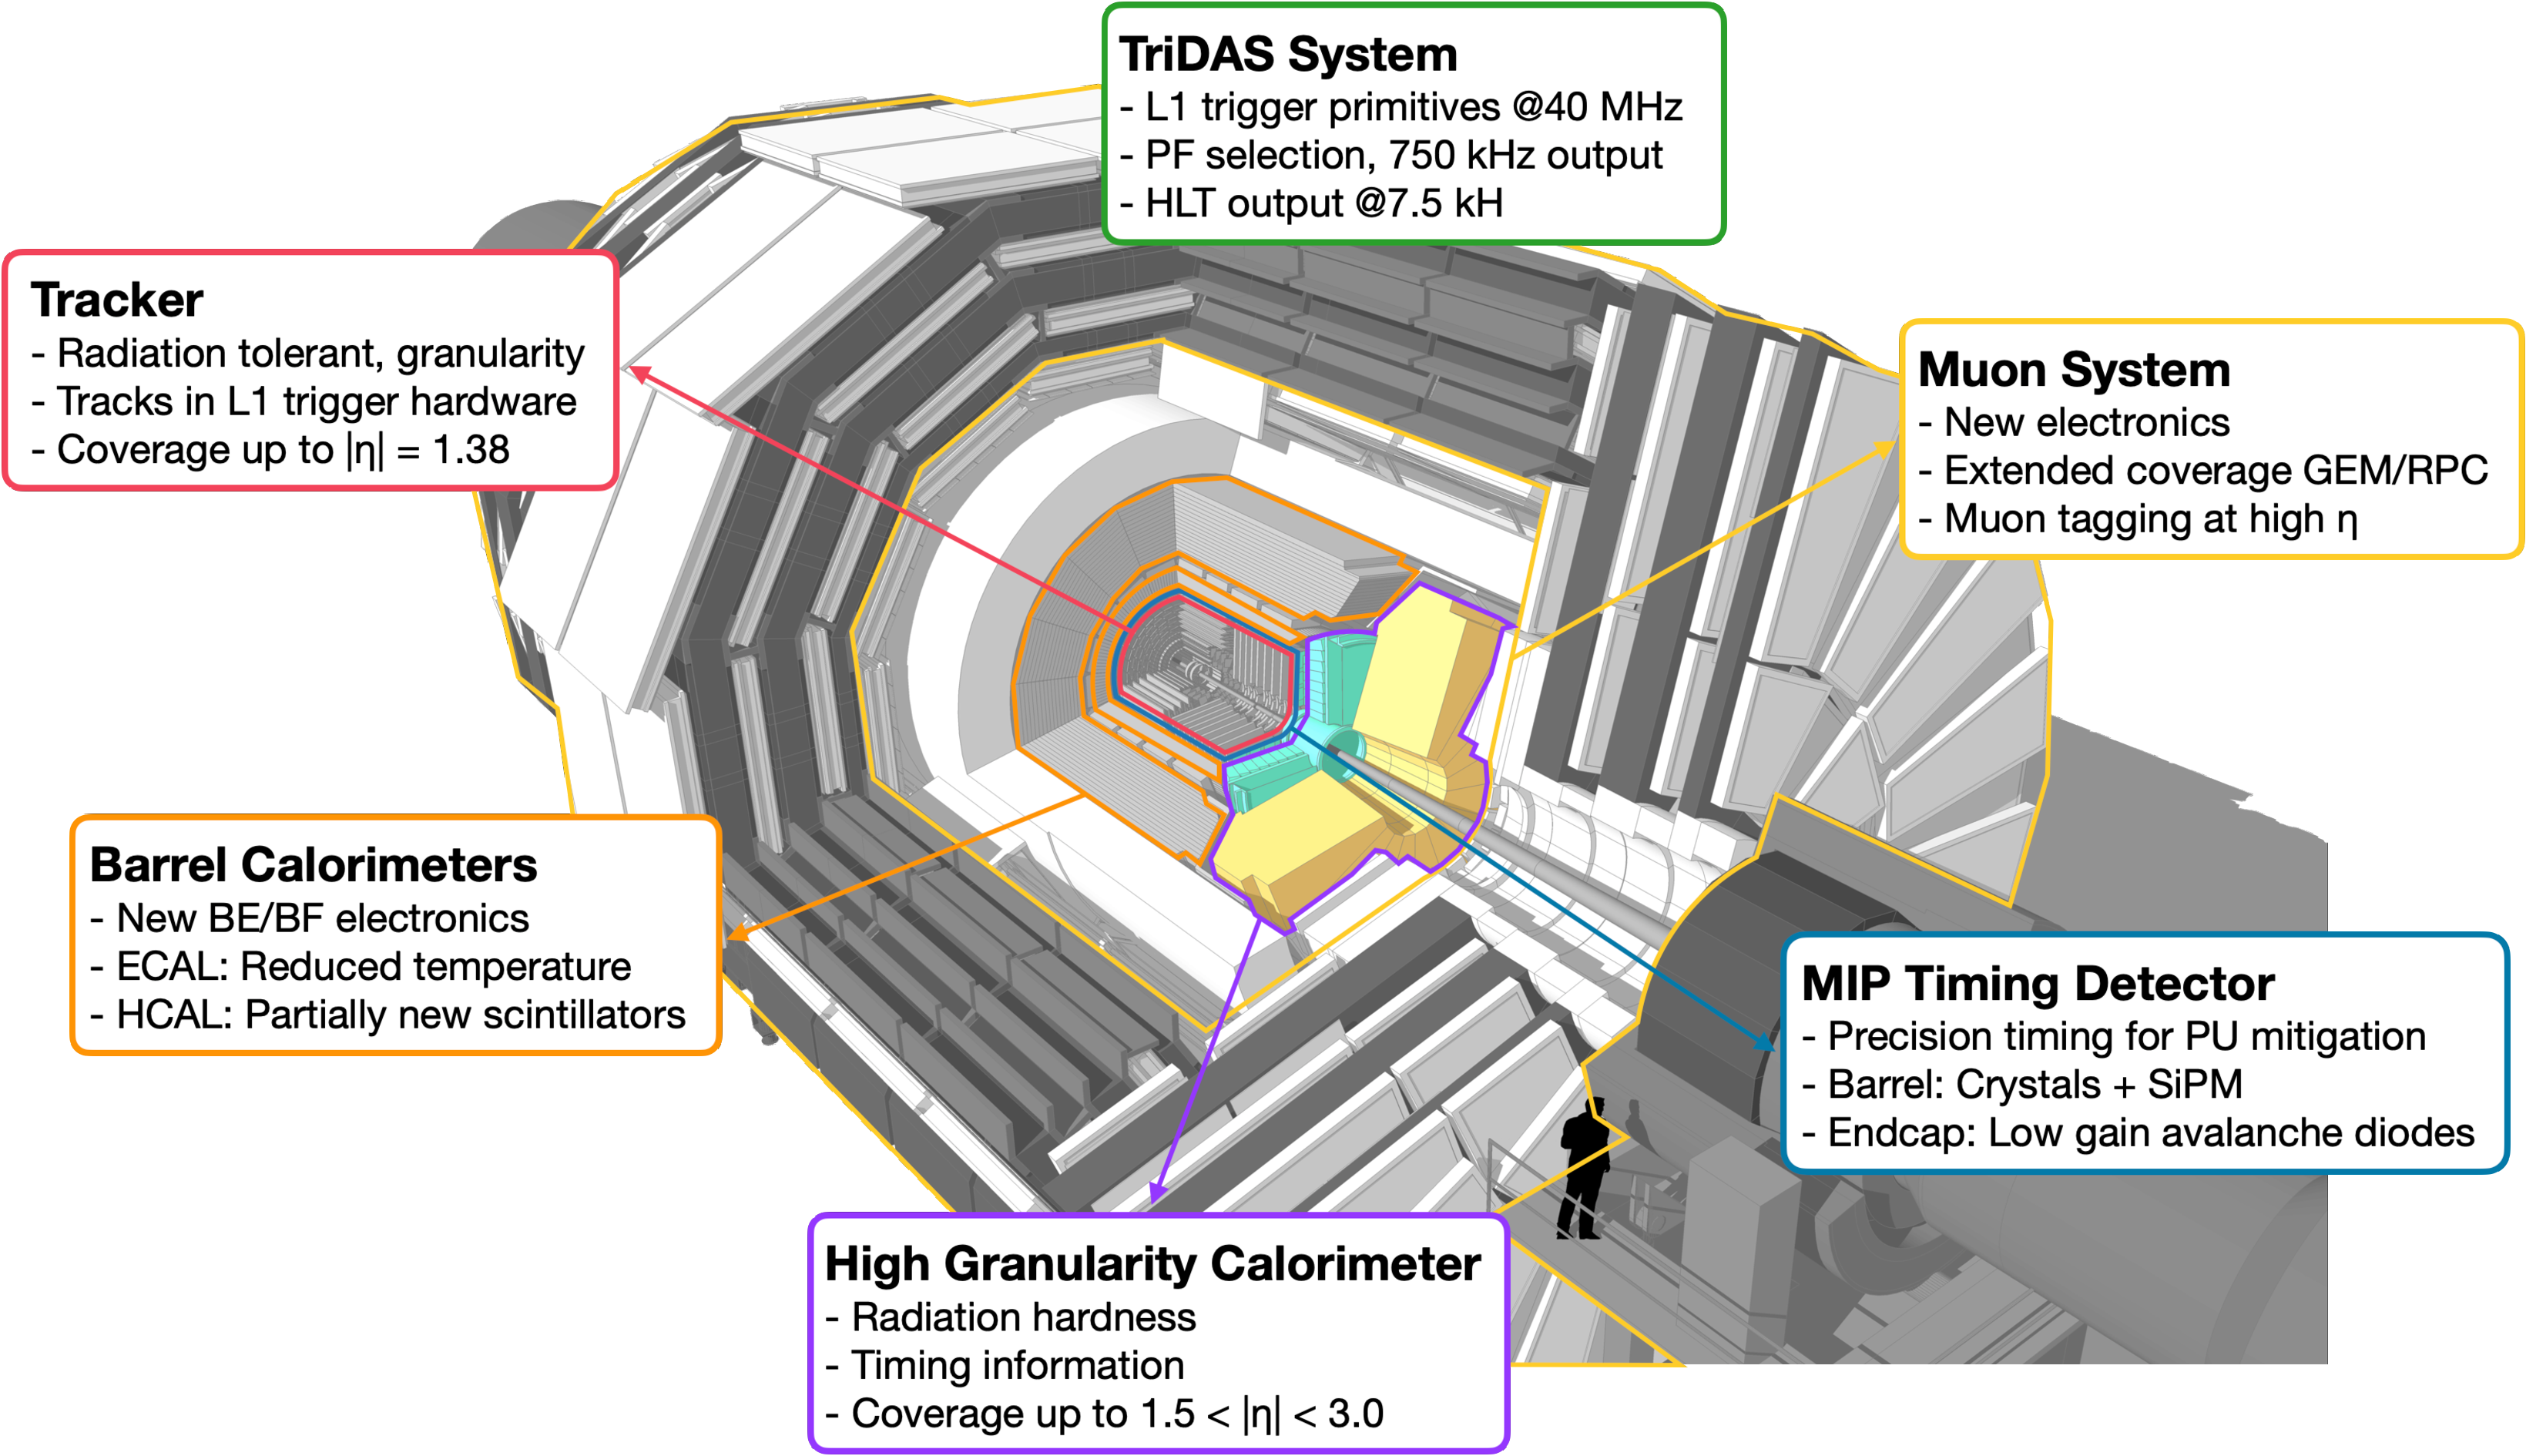
\includegraphics[width=0.95\linewidth]{Figures/HGCAL/CMSUpgrades.pdf}
    \caption{Cross section of the CMS detector with the indication of the upgrades foreseen for the HL-LHC.}
    \label{fig:CMSUpgrade}
\end{figure}

\paragraph{Tracker and pixel}
To enhance the detector granularity and reconstruction performance while minimising the material budget, the tracking system will see a full replacement of its inner and outer parts. Both sub-systems will be equipped with more radiation hard sensors and electronics, specified to withstand the increased particle fluence and offer high tracking efficiency under higher particle rates.
The modules will be designed to provide the tracking information to the Level-1 trigger at 40~MHz for all tracks with $p_T\geq$~GeV, reducing the fake rate at the earliest stage of the event selection.~\cite{CERN-LHCC-2017-009}.

\paragraph{MIP Timing Detector}
Multiple MIP timing detectors (MTD) will be positioned in front of the barrel and endcap calorimeters. This additional layer will improve the timing information on charged candidates, which is crucial for disentangling the approximately 200~PU interactions foreseen per bunch crossing. It will also provide new capabilities for charged hadron identification and for long-lived particles searches~\cite{CMS:2667167}.

\paragraph{Barrel Calorimeters}
The electron and hadron barrel calorimeters will undergo minor changes, unlike the endcap calorimeters which will be totally replaced.
Upgrades to the ECAL and HCAL barrel electronic read-out systems are planned: in particular the replacement of the front-end electronics of the ECAL barrel, and the replacement of the off-detector electronics of both ECAL and HCAL barrel~\cite{CERN-LHCC-2017-011}.

\paragraph{Endcap Calorimeters}
The electromagnetic and hadronic endcap calorimeters are not foreseen to tolerate radiation levels higher than those which correspond to an integrated luminosity of about 500~$\textnormal{fb}^{-1}$ and must be replaced by a new sampling calorimeter, the HGCAL, comprising electromagnetic and hadronic sections with excellent transverse and longitudinal segmentation. The HGCAL will provide three-dimensional images of the particle showers, enhancing particle separation and identification~\cite{CERN-LHCC-2017-023}. A more complete description of the future HGCAL is provided in Section~\ref{sec:The High-Granularity Calorimeter}.

\paragraph{Muon system}
The redundancy of the current muon detection system, comprising DTs, RPCs, and CSCs, will be augmented by the installation of Gas Electron Multiplier (GEM) chambers and a new generation of RPCs with improved timing resolution. These enhancements will extend coverage up to $|\eta|=2.8$ and $|\eta|=2.4$, respectively~\cite{CERN-LHCC-2017-012}.

\paragraph{Trigger and DAQ}
In order to cope with much higher data rates due to the increased pile-up, the trigger and data acquisition systems will be completely replaced. The L1 trigger rate will be about 750~kHz (compared to the current 100~kHz), to exploit the full potential of the increase in peak instantaneous luminosity.
The Level-1 hardware trigger will be redesigned to include the additional information from the Tracker and the HGCAL, requiring a longer processing time of 12.5~$\mu$s latency. 
The use of modern FPGAs and processors, high-speed optical links for data aggregation and sophisticated reconstruction ML-based algorithms are some of the additional features of the upgraded Trigger system~\cite{CERN-LHCC-2017-013}-\cite{CERN-LHCC-2017-014}.

\bigbreak

Figure~\ref{fig:CMSUpgrade} illustrates a cross-section of the CMS detector, outlining the planned upgrades for the HL-LHC. For each subdetector, the the main modified features are described: the Tracker, TriDAS system and the forward calorimeters will undergo complete replacement, while the MIP timing detector, the barrel calorimeters, and the muon system will constitute new parts or modules that are not part of the current CMS design.
% https://cds.cern.ch/record/2628519

%%%%%%%%%%%%%%%%%%%%%%%%%%%%%%%%%%%%%%%%%%%%%%%%%%%%%%%%%%%%%%%%%%%%%%%%%%%%%%%%%%%%%%%%%%%%
%%%%%%%%%%%%%%%%%%%%%%%%%%%%%%%%%%%%%%%%%%%%%%%%%%%%%%%%%%%%%%%%%%%%%%%%%%%%%%%%%%%%%%%%%%%%
%%%%%%%%%%%%%%%%%%%%%%%%%%%%%%%%%%%%%%%%%%%%%%%%%%%%%%%%%%%%%%%%%%%%%%%%%%%%%%%%%%%%%%%%%%%%
%%%%%%%%%%%%%%%%%%%%%%%%%%%%%%%%%%%%%%%%%%%%%%%%%%%%%%%%%%%%%%%%%%%%%%%%%%%%%%%%%%%%%%%%%%%%

\section{The High-Granularity Calorimeter}
\label{sec:The High-Granularity Calorimeter}

Among the CMS detector updates, one of the most ambitious projects is the High Granularity Calorimeter (HGCAL), a novel sampling calorimeter designed to replace the existing CMS endcap calorimeter to maintain an excellent physics performance under the high pile-up and harsh radiation environment of the HL-LHC.
The existing Endcap Calorimeters (CE) of the CMS detector were designed to sustain a total integrated luminosity of 500 $\textnormal{fb}^{-1}$, which is expected to be exceeded shortly after the beginning of the HL-LHC phase. 
The transparency of the lead-tungstate ($\textnormal{PbWO}_4$) crystals, already degraded during Run-II operations, would not survive the unprecedented radiation flux typical of the HL-LHC environment and the physics performance would degrade to unacceptable levels.
It is therefore necessary to replace the current calorimeter endcaps with a new profoundly different calorimeter, characterised by high radiation tolerance, highly granular energy deposit, and good time resolution to adequately treat pile-up in the offline event reconstruction.

\bigbreak

The HGCAL will comprise both electromagnetic and hadronic sections, covering the pseudorapidity region $1.5<|\eta|<3.0$, and weighing 215 tonnes per endcap. It will consist of 47 layers divided into two compartments:
\begin{itemize}
    \item Electromagnetic Compartment (CE-E), featuring 26 active layers, alternated with CuW, Cu, and Pb absorbers;
    \item Hadronic Compartment (CE-H), composed of 21 layers exploiting stainless steel as passive material.
\end{itemize}

\begin{figure}
    \centering
    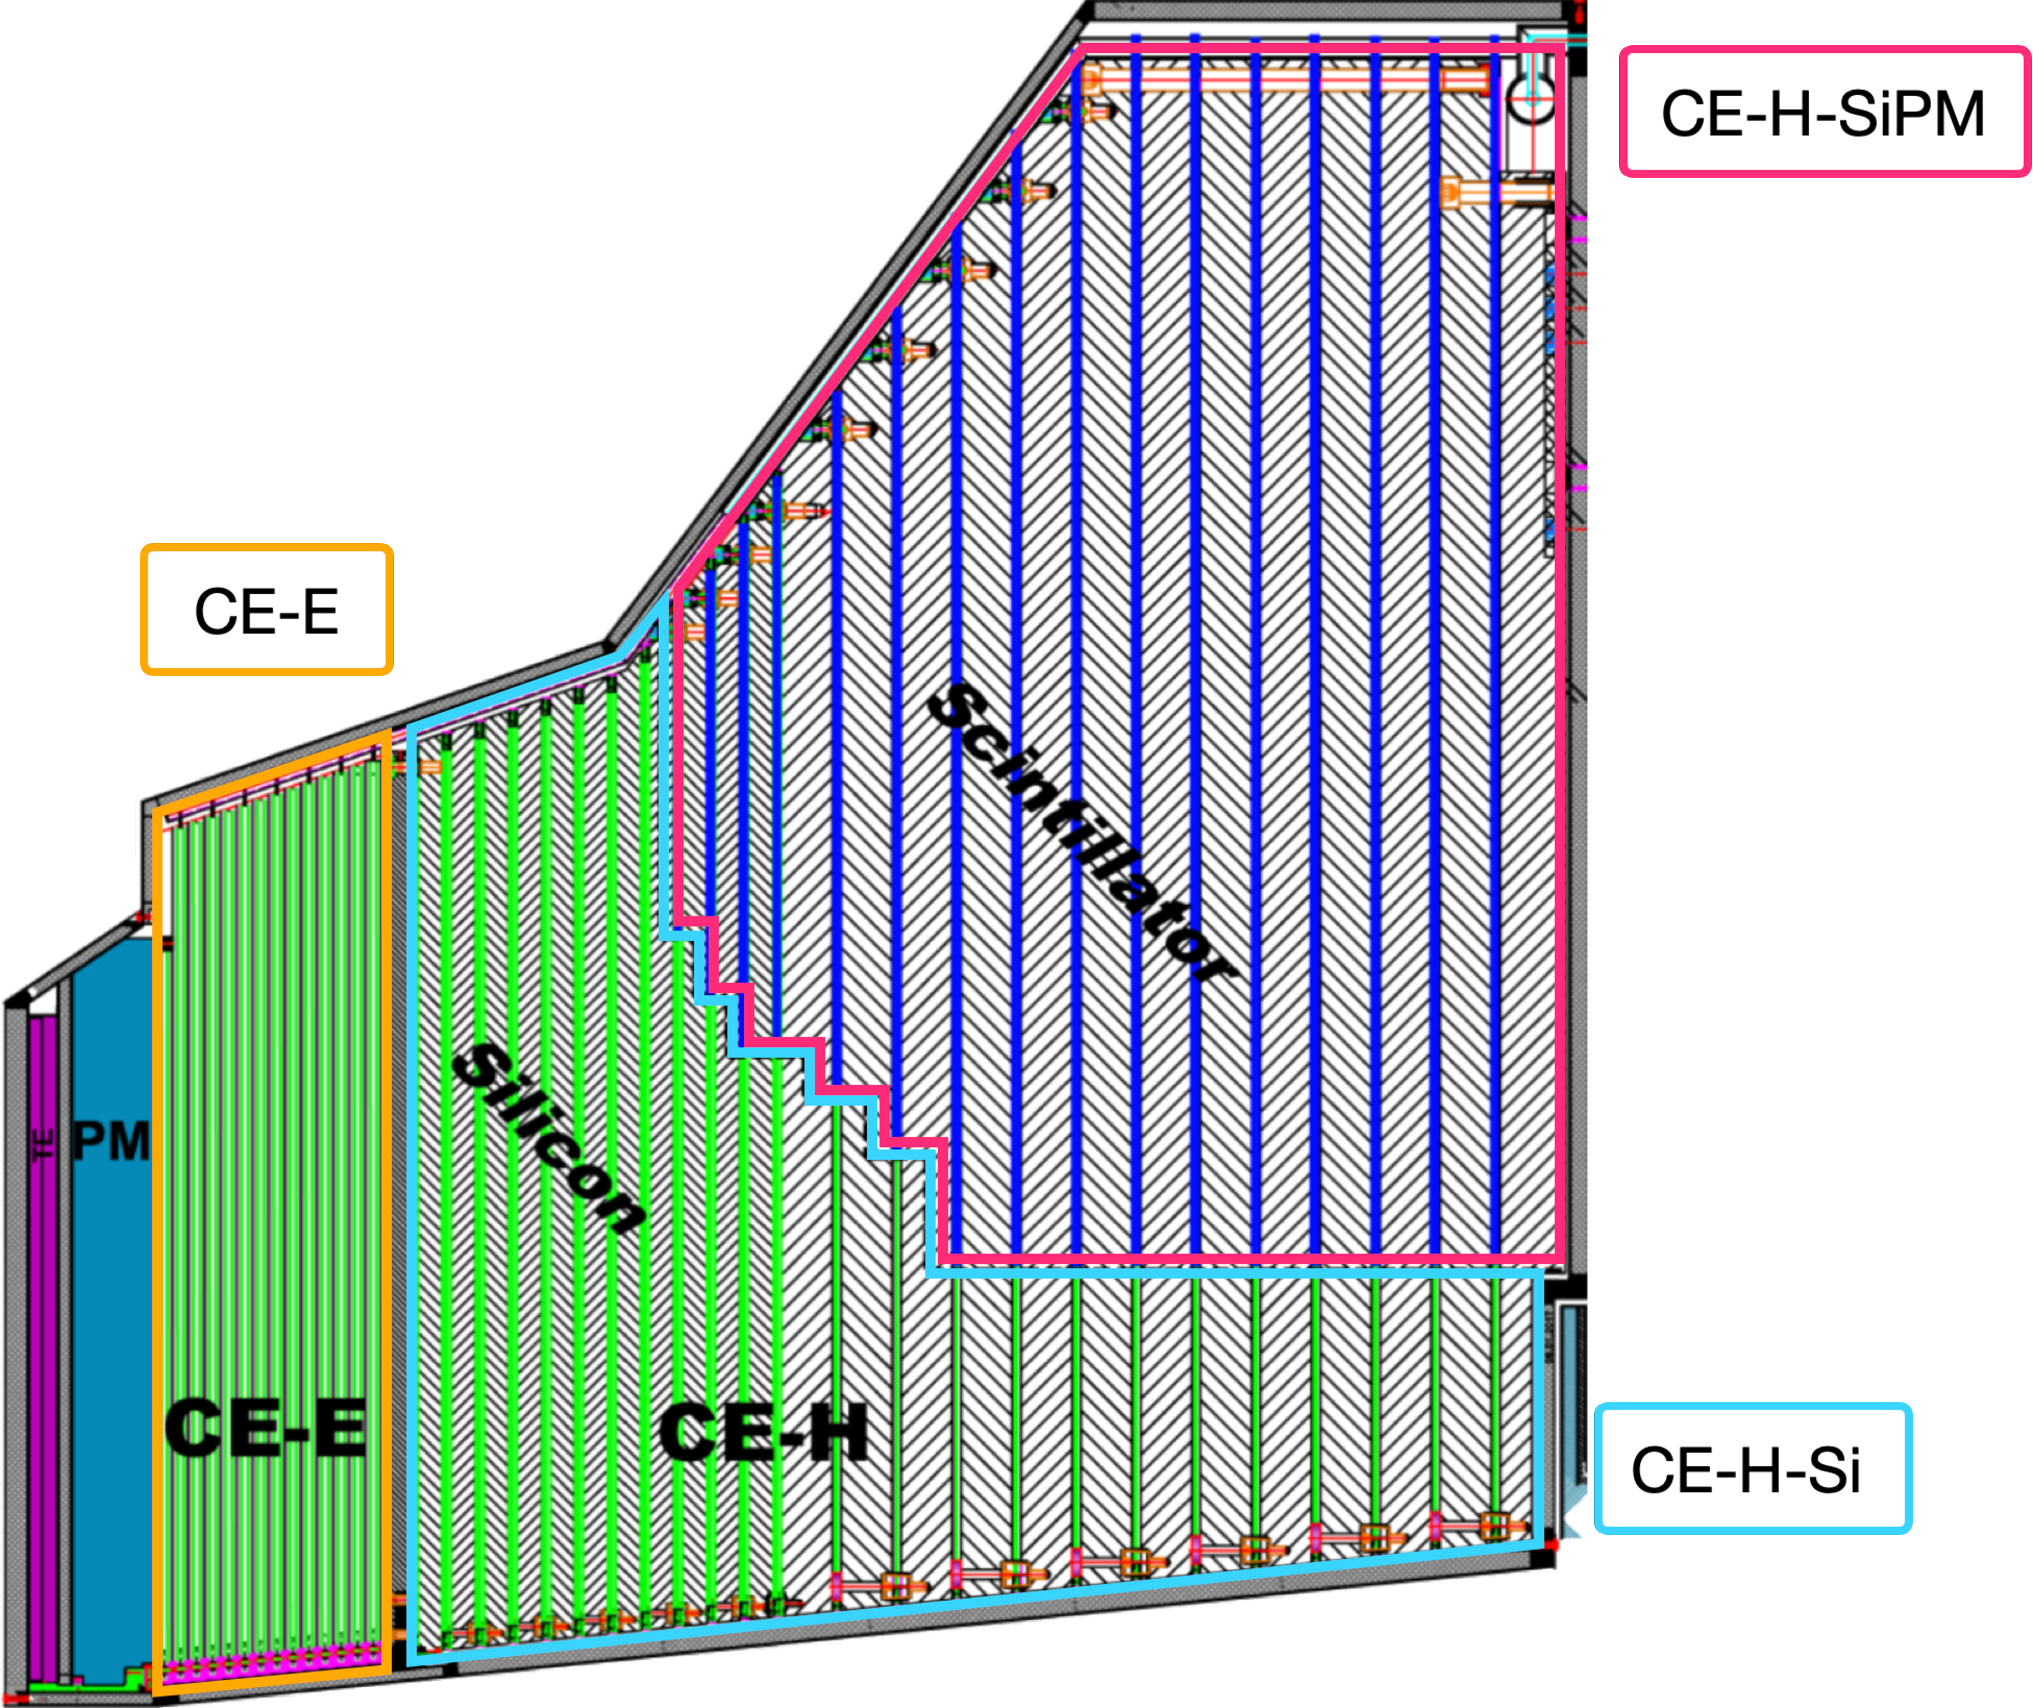
\includegraphics[width=0.6\linewidth]{Figures/HGCAL/HGCALLayers.pdf}
    \caption{Cross section view of the HGCAL. The CE-E and front CE-H compartments comprise silicon-based components. In its latest design, the HGCAL features 47 layers divided into two regions: 26 silicon-based layers for the Electromagnetic Compartment (CE-E), 21 layers for the Hadronic Compartment (CE-H), using silicon (CE-H-Si) and scintillator-based (CE-H-SiPM) active material. The expected coverage of the HGCAL will range from $|\eta|=1.5$ up to $|\eta|=3.0$.}
    \label{fig:HGCALLayers}
\end{figure}

The number of longitudinal samplings has been designed as a trade-off between the best shower reconstruction and the engineering requirements of the mechanical structure. 
To meet the radiation hardness requirements, the CE-E and the front part of the CE-H will employ silicon as active material, for a total area of about 600~$\textnormal{m}^2$ to be covered. 
In the remaining lower radiation regions of the CE-H, at about 4~m from the interaction point, segmented plastic scintillators with silicon photomultipliers (SiPM) for the read-out will be used as active material. 
Square scintillator tiles with sizes ranging from 4~$\textnormal{cm}^2$ up to 30~$\textnormal{cm}^2$ will be installed, for a total of about 400~$\textnormal{m}^2$ of the active area covered in scintillators.
This configuration amounts to approximately 10 nuclear radiation lengths ($\lambda_n$), divided into 1.3~$\lambda_n$ for the CE-E and 8.5~$\lambda_n$ for the CE-H. The CE-E alone will extend for a total of 27.7 radiation-lengths ($X_0$).

A longitudinal cross section of the HGCAL is shown in Figure~\ref{fig:HGCALLayers}, where the multiple layers of the Electromagnetic and Hadronic Compartments are visible, along with the different active materials used in the two regions.

\bigbreak

\begin{figure}
    \centering
    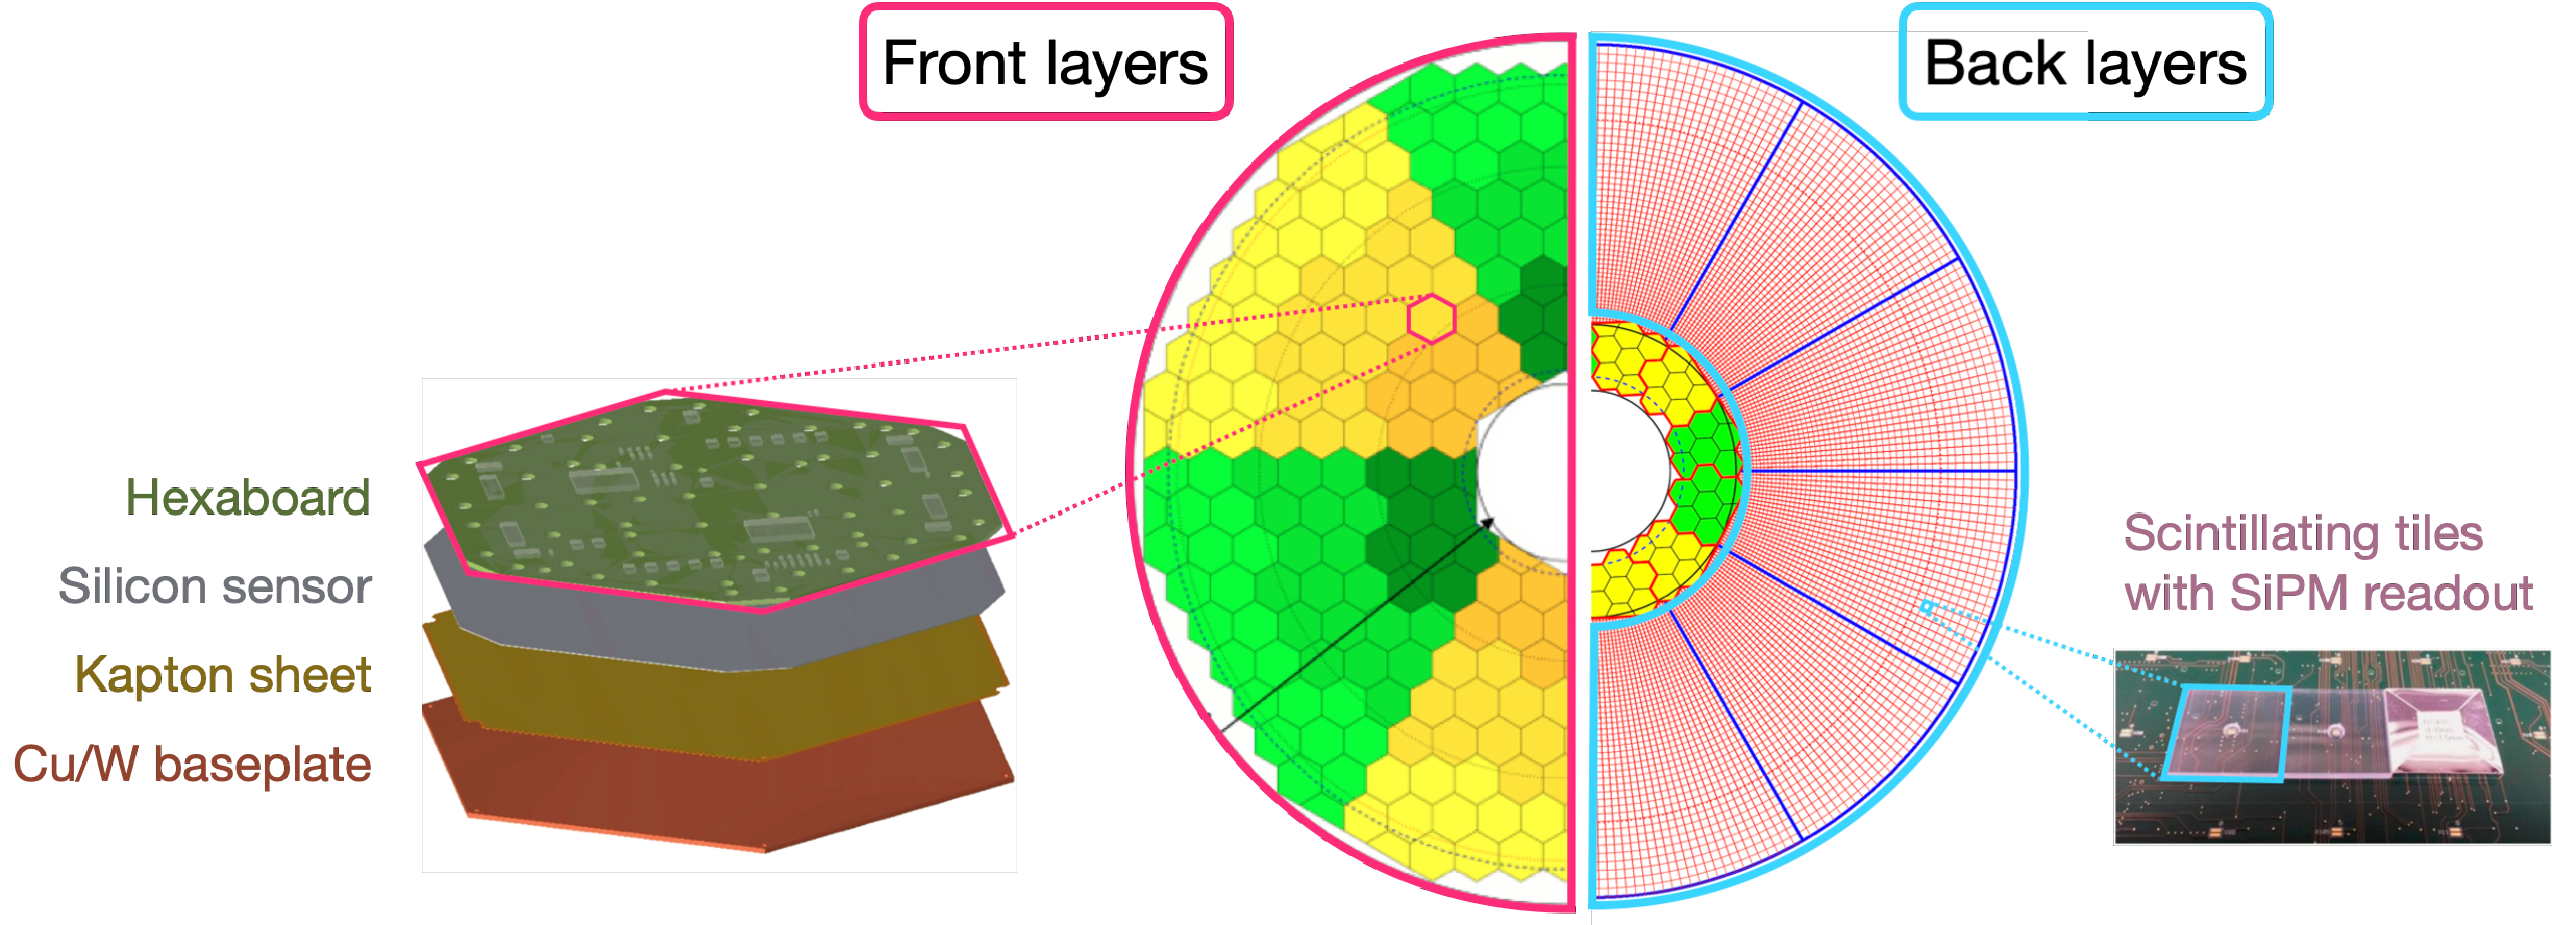
\includegraphics[width=0.9\linewidth]{Figures/HGCAL/FrontBackLayers.pdf}
    \caption{Schematic view of the arrangement of the hexagonal silicon modules in the front layers composing the CE-E and CE-H-Si (left) and of the scintillator tiles employed in the low radiation back layers of the CE-H-SiPM (right).}
    \label{fig:FrontBackLayers}
\end{figure}

In order to cover the area in the most cost-effective manner, the hexagonal geometry for the silicon sensors will be exploited. 
The 8-inch hexagonal sensors will have an active thickness of 120, 200, or 300~$\mu$m, depending on the detector region: thinner sensors will be employed in higher fluence regions in order to optimise the charge collection and reduce the leakage current.
Each module will comprise several hexagonal single read-out diodes, or \textit{cells}, with two different sizes: 0.52~$\textnormal{cm}^2$ for the 120~$\mu$m thickness sensors, and 1.18~$\textnormal{cm}^2$ for the 200 and 300~$\mu$m thickness sensors.
Depending on the size of the read-out cells, two regions will be defined, namely a \textit{high-density} and \textit{low-density} region.
The transition region will be at a radius of 70~cm, corresponding to $|\eta| \simeq 2.15$. The high-density, i.e. more granular, region is located at higher pseudorapidity, where a larger number of tracks is expected to enter the HGCAL.
The design, production, and validation of the hexagonal sensors, hereafter referred to as \textit{modules}, is one of the most challenging aspects of the HGCAL project. In total, six million individual cells will be read out in the final detector operation, organised in 27,000 modules.
A more detailed discussion about silicon as active material and the structure of the HGCAL modules is given in Section~\ref{sec:Silicon Modules}. 
In the CE-E, the silicon modules will be used to create self-supporting sandwich structures which are commonly referred to as \textit{cassettes}; the modules will be installed on both sides of a copper cooling plate and will be closed with lead plates.

In the low radiation CE-H-SiPM compartment, the scintillating material, coupled to SiPMs read-out, will be transversely segmented in square shapes. The scintillating cells will have variable sizes, from 4~$\textnormal{cm}^2$ in the inner region to 32~$\textnormal{cm}^2$ in the outer region. 
The scintillator modules will be composed of tileboard Printed Circuit Boards (PCBs) with different sizes and shapes. Each tileboard will host from 48 to 96 scintillator tiles, individually wrapped into a reflecting layer and characterised by a cavity to contain the SiPM. Each detector on the board will be equipped with an ultraviolet LED for the calibration and monitoring of the SiPM gain. 
In total, 240,000 scintillator channels will be used, organised in 4,000 boards.

This geometrical configuration amounts to a total active area of 620~$\textnormal{m}^2$ and 370~$\textnormal{m}^2$ for the CE-E and CE-H compartments respectively, and provides a compact and cost-effective way to build the entire calorimeter at a reasonable cost while meeting the strict radiation requirements in the high pseudorapidity region.
To maintain a reasonable detection of MIPs over the detector lifetime and ensure a good signal-to-noise ratio, the effects of radiation damage must be minimised. To achieve this goal, the HGCAL will have to be operated at a constant temperature of -30~$^{\circ}$C or lower, obtained through a dedicated $\textnormal{CO}_2$ cooling system directly implemented in the copper base plate. 

The arrangement of the silicon modules in the CE-E and CE-H-Si (front layers) is represented in the left part of Figure~~\ref{fig:FrontBackLayers}, while the right part shows the scintillator tiles employed in the CE-H-SiPM region (back layers).

\bigbreak

The HGCAL design guarantees coverage in the pseudorapidity range $1.5 < |\eta| < 3.0$, featuring both highly granular lateral and longitudinal segmentation. 
The enhanced lateral granularity, combined with the dense absorbers, allows for effective individual shower containment and particle discrimination within the detector. Moreover, the finely segmented longitudinal structure enhances PU rejection, particle identification, and energy resolution. Because of these features, the HGCAL is often referred to as an \textit{imaging}, or 5D, calorimeter, the five dimensions corresponding to the three-dimensional spatial information provided by the fine voxels, the energy deposit in each active material segment, and the timing information with an expected resolution of $\mathcal{O}$(10~ps).

\subsection{Silicon Modules}
\label{sec:Silicon Modules}

\begin{figure}
    \centering
    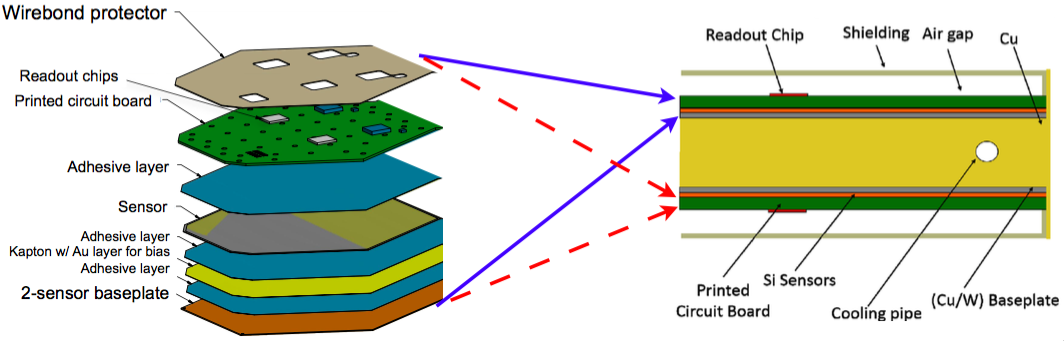
\includegraphics[width=0.9\linewidth]{Figures/HGCAL/ModuleDesign.png}
    \caption{Composition of a silicon module and placement in the copper plate. Each module is a stack of different layers, starting with a baseplate at the bottom, covered with a gold plated Kapton foil on which stands the silicon sensor. A protected PCB with read-out chip is placed on top.}
    \label{fig:ModuleDesign}
\end{figure}

The choice of silicon as the active material in the HGCAL modules is driven by the stringent constraints imposed by the expected physics performance and operating detector conditions. 
Silicon sensors ensure at the same time the detection of minimum ionizing particles (MIPs) and precise measurements of high-energy showers, both crucial for the HGCAL operation efficiency. The former is essential for \textit{in situ} calibrations of the detector, the latter can be ensured only with full containment of the showers, which relies on the detector compactness achieved through thin silicon modules and a proper mixture of absorbers.
In addition, silicon sensors offer a rapid signal response of $\mathcal{O}$(10~ns), necessary to keep up with the expected 40 MHz rates at the HL-LHC. Finally, silicon module production benefits from well-established large-scale industrial capabilities, allowing for relatively short production times.

\bigbreak

The HGCAL will require approximately 27,000 silicon detector modules to be assembled and installed in its electromagnetic (CE-E) section and part of the hadronic (CE-H) section.
Each module consists of stacked layers comprising the PCB, labelled \textit{hexaboard}, where the front-end electronics will be installed, the silicon sensor, and a gold-plated Kapton sheet providing high-voltage connection to the sensor back-plane and electrical insulation. The baseplate, made of materials such as CuW or Cu, provides enough rigidity to support the module whilst minimising the total radiation length and dissipating the heat through the dedicated cooling system.
The silicon modules will be segmented into 192 cells for the low-density (LD) region, and in 432 cells, for the high-density (HD) region. The hexagonal cells will act as independent diodes with a separate read-out channel.

A schematic view of the structure of a typical HGCAL module is given in Figure~\ref{fig:ModuleDesign}.

\subsection{Plastic Scintillation Tiles}
\label{sec:Plastic Scintillation Tiles}

The remaining portion of the CE-H compartment will incorporate scintillator as the active material. Given their lower radiation tolerance, plastic scintillators will be employed in regions where the integrated dose remains low-enough ($<3$~kGy) to maintain optimal performance throughout the entire lifespan of the HL-LHC. 
This approach will also ensure effective muon identification in the $\eta>2.4$ region, where muon chambers are unavailable.

The scintillator will be crafted into small squared tiles, with the scintillation light reflected by a wrapping foil and directly read-out by a SiPM optically coupled through a small \textit{dimple} in the centre of one face of each tile. The SiPMs will be mounted on printed circuit boards, and matched to the appropriate tiles. 
The system is illustrated in Figure~\ref{fig:ScintillatorTiles}.

In conformity with the CMS endcap's geometry, the scintillator cells will be arranged in an $r,\phi$ grid. As a result, cells closer to the beam line will be significantly smaller (4~$\textnormal{cm}^2$) than those at the outer edge (32~$\textnormal{cm}^2$). 
The area instrumented with scintillators will be subdivided into tile-modules consisting of a tileboard and the scintillator tiles. These tile-modules will then be connected to form a 10~$^{\circ}$ detector unit. Six units will be placed next to each other and combined with silicon modules into cassettes, covering 60~$^{\circ}$ each. Finally, six cassettes will collectively complete the calorimeter layer around the beam pipe.

\begin{figure}
    \centering
    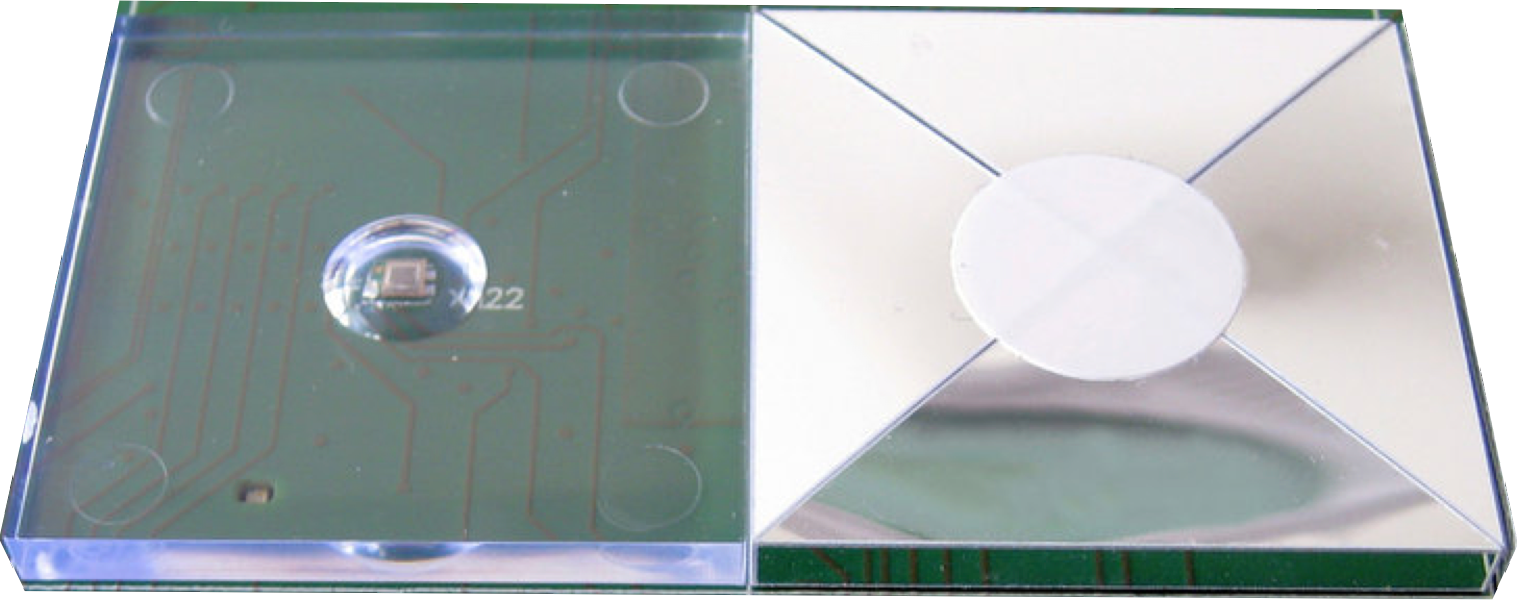
\includegraphics[width=0.5\linewidth]{Figures/HGCAL/ScintillatorTiles.pdf}
    \caption{Example of two $3\times3$~$\textnormal{cm}^2$ scintillator tiles with a central dimple, unwrapped (left) and wrapped (right), mounted on a PCB housing one SiPM per tile, used as a prototype for the HGCAL project.}
    \label{fig:ScintillatorTiles}
\end{figure}

%%%%%%%%%%%%%%%%%%%%%%%%%%%%%%%%%%%%%%%%%%%%%%%%%%%%%%%%%%%%%%%%%%%%%%%%%%%%%%%%%%%%%%%%%%%%
%%%%%%%%%%%%%%%%%%%%%%%%%%%%%%%%%%%%%%%%%%%%%%%%%%%%%%%%%%%%%%%%%%%%%%%%%%%%%%%%%%%%%%%%%%%%
%%%%%%%%%%%%%%%%%%%%%%%%%%%%%%%%%%%%%%%%%%%%%%%%%%%%%%%%%%%%%%%%%%%%%%%%%%%%%%%%%%%%%%%%%%%%
%%%%%%%%%%%%%%%%%%%%%%%%%%%%%%%%%%%%%%%%%%%%%%%%%%%%%%%%%%%%%%%%%%%%%%%%%%%%%%%%%%%%%%%%%%%%

\section{The HGCAL Front-End Electronics}
\label{sec:The HGCAL Front-End Electronics}

One of the most challenging aspects in the design of the HGCAL silicon and scintillator modules is the front-end (FE) electronics. 

The FE electronics is responsible for several critical functions within the HGCAL system. It measures and digitises the charge deposited in the silicon sensor pads or generated in the SiPMs, providing precise time measurements for the pulses. It transmits the digitised data to the back-end (BE) electronics located in the service cavern. It also computes, at each bunch crossing, the digital sums of neighbouring cells, tailored to the specific cell sizes (4 cells for 1.18~$\textnormal{cm}^2$ HD silicon sensors, 3 cells for 0.52~$\textnormal{cm}^2$ LD silicon sensors, and 2 cells for scintillator tiles); the data are transmitted to the trigger BE electronics to build trigger primitives.

\begin{figure}
    \centering
    \includegraphics[width=0.95\linewidth]{Figures/HGCAL/Hexaboards.pdf}
    \caption{Plan view of two hexaboards housing 6 High Density (HD) HGCROC read-out chips: each chip is connected to 72 hexagonal cells. The connector will be used for the assembly of the motherboard, containing the ECON-D and ECON-T concentrator chips.}
    \label{fig:Hexaboards}
\end{figure}

Besides the unprecedented read-out segmentation, the performance requirements for the FE electronics are extremely stringent, particularly for the silicon part of the detector:
\begin{itemize}
    \item [-] Low noise, below 2,000 electrons for a 65~pF capacitance pad to allow for MIP visibility during the whole operation.
    \item [-] Large dynamic range, spanning from approximately 0.2~fC to 10~pC, equivalent to 16 bits; this range enables at the same time the detection of MIPs in the silicon sensors and the recording of high-energy deposits from electromagnetic showers. 
    \item [-] Integral linearity above 1$\%$ across the entire dynamic range.
    \item [-] Timing information with precision better than 100~ps for pulses above 12~fC, corresponding to about 3~MIPs in the 300~$\mu$m silicon sensors.
    \item [-] Fast shaping time (peaking-time $<20$~ns) to minimise the out-of-time pileup; the pulse should be dropped to less than 20$\%$ by the start of the next bunch crossing.
    \item [-] On-detector digitisation and data processing for zero suppression, linearisation and summing of the trigger data.
    \item [-] Maximum latency of 36~bunch crossings for the trigger primitives at the detector output.
    \item [-] Buffering of the data to accommodate the 12.5~$\mu$ms L1 trigger latency.
    \item [-] High-speed read-out links to interface with 10~Gb/s low-power GBT (LpGBT) serialiser.
    \item [-] Low power budget ($<20$~mW per channel), typically limited by cooling power.
\end{itemize}

Following the LHC data-taking conditions, the acquisition chain must handle consecutive event arrivals at 40~MHz without data erasure.
Moreover, the FE electronics will face a harsh radiation environment which will reach 200~Mrad at the end of life and require extremely high radiation tolerance.

\bigbreak

In the HGCAL FE architecture, the very first step of the electronic chain is the HGCal Read-Out Chip (HGCROC), an Application-specific integrated circuit (ASIC) featuring state-of-the-art electronic components for the read-out of the individual cells. The HGCROC measures at 40~MHz frequency the charge and the time of arrival of each particle crossing the HGCAL cells. 
The HGCROC read-out chips, together with the linear voltage regulators (LVR) and other passive and service components, are mounted on a hexagonal module PCB, called \textit{hexaboard}, which is glued onto the silicon sensor.
The HGCROC is directly bonded through a ball-grid array to the hexaboard and has multiple channels connected to individual cells. 
Two different chip packages have been specifically designed for the HD and LD hexaboards, hosting 6 HD HGCROC and 3 LD HGCROC chips respectively.
Imprinted on the hexaboard are also the pads for connections to the next board in the chain, labelled \textit{motherboard}. These connections also supply the LV, receive and transmit signals and data. 

\bigbreak

The next level of the FE electronics includes the concentrators, located on the motherboards sitting 1.6~mm above the headboards. Each motherboard serves from one to six modules, depending on the occupancy of the sensors. The surfaces including the components of the hexaboard and of the motherboard face each other to reduce the overall thickness. 
The architecture of the very FE electronics chain on the hexaboards is summarised in Figure~\ref{fig:Hexaboards}. 

%%%%%%%%%%%%%%%%%%%%%%%%%%%%%%%%%%%%%%%%%%%%%%%%%%%%%%%%%%%%%%%%%%%%%%%%%%%%%%%%%%%%%%%%%%%%
%%%%%%%%%%%%%%%%%%%%%%%%%%%%%%%%%%%%%%%%%%%%%%%%%%%%%%%%%%%%%%%%%%%%%%%%%%%%%%%%%%%%%%%%%%%%
%%%%%%%%%%%%%%%%%%%%%%%%%%%%%%%%%%%%%%%%%%%%%%%%%%%%%%%%%%%%%%%%%%%%%%%%%%%%%%%%%%%%%%%%%%%%
%%%%%%%%%%%%%%%%%%%%%%%%%%%%%%%%%%%%%%%%%%%%%%%%%%%%%%%%%%%%%%%%%%%%%%%%%%%%%%%%%%%%%%%%%%%%

\section{The HGCROC3 architecture}
\label{sec:The HGCROC3 architecture}

\begin{figure}
    \centering
    \includegraphics[width=0.75\linewidth]{Figures/HGCAL/TwoHalves.pdf}
    \caption{Layout of the HGCROC3 ASIC: the chip is divided into two symmetrical parts. The voltage reference is positioned near the chip edge, and the ADC reference and TDC controls are located in the central region.}
    \label{fig:TowHalves}
\end{figure}

With an extraordinary technical effort to meet all the FE electronics requirements, the HGCROC3 is the final version of the ASIC specifically designed by the CMS Collaboration, in collaboration with the Omega Microelectronics Center at École Polytechnique, to read-out the modules of the future HGCAL. 
Two versions of the same read-out architecture have been developed, for the silicon (Si) and the scintillator tiles (SiPM) sections, where the latter is obtained by only adding a current conveyor and adapting the preamplifier of the silicon variant. The Si version is configured in the two different packages, for the read-out of HD and LD modules, while the SiPM version is only deployed in the LD package.

\bigbreak

The main function of the HGCROC3 is to measure and digitise the charge deposit and provide high precision time information from the particles crossing the detector layers. It is also able to compute the energy sum of neighbouring cells in order to contribute to the L1 trigger decision. 
The chip features 78 channels, each consuming less than 15 mW power, and is designed in a radiation-hardened 130~nm CMOS technology. Among the channels, 72 serve as standard cells read-out, 2 function as calibration cells read-out, and the remaining 4 channels are not connected to any sensor cells, serving for common-mode noise estimation. 

The layout is symmetrically divided into two parts, or \textit{halves}, as shown in Figure~\ref{fig:TowHalves}.
In Figure~\ref{fig:Architecture} a schematics of the inner architecture of the ASIC is presented: the structure and characteristics of each component are described in the following paragraphs.

\begin{figure}
    \centering
    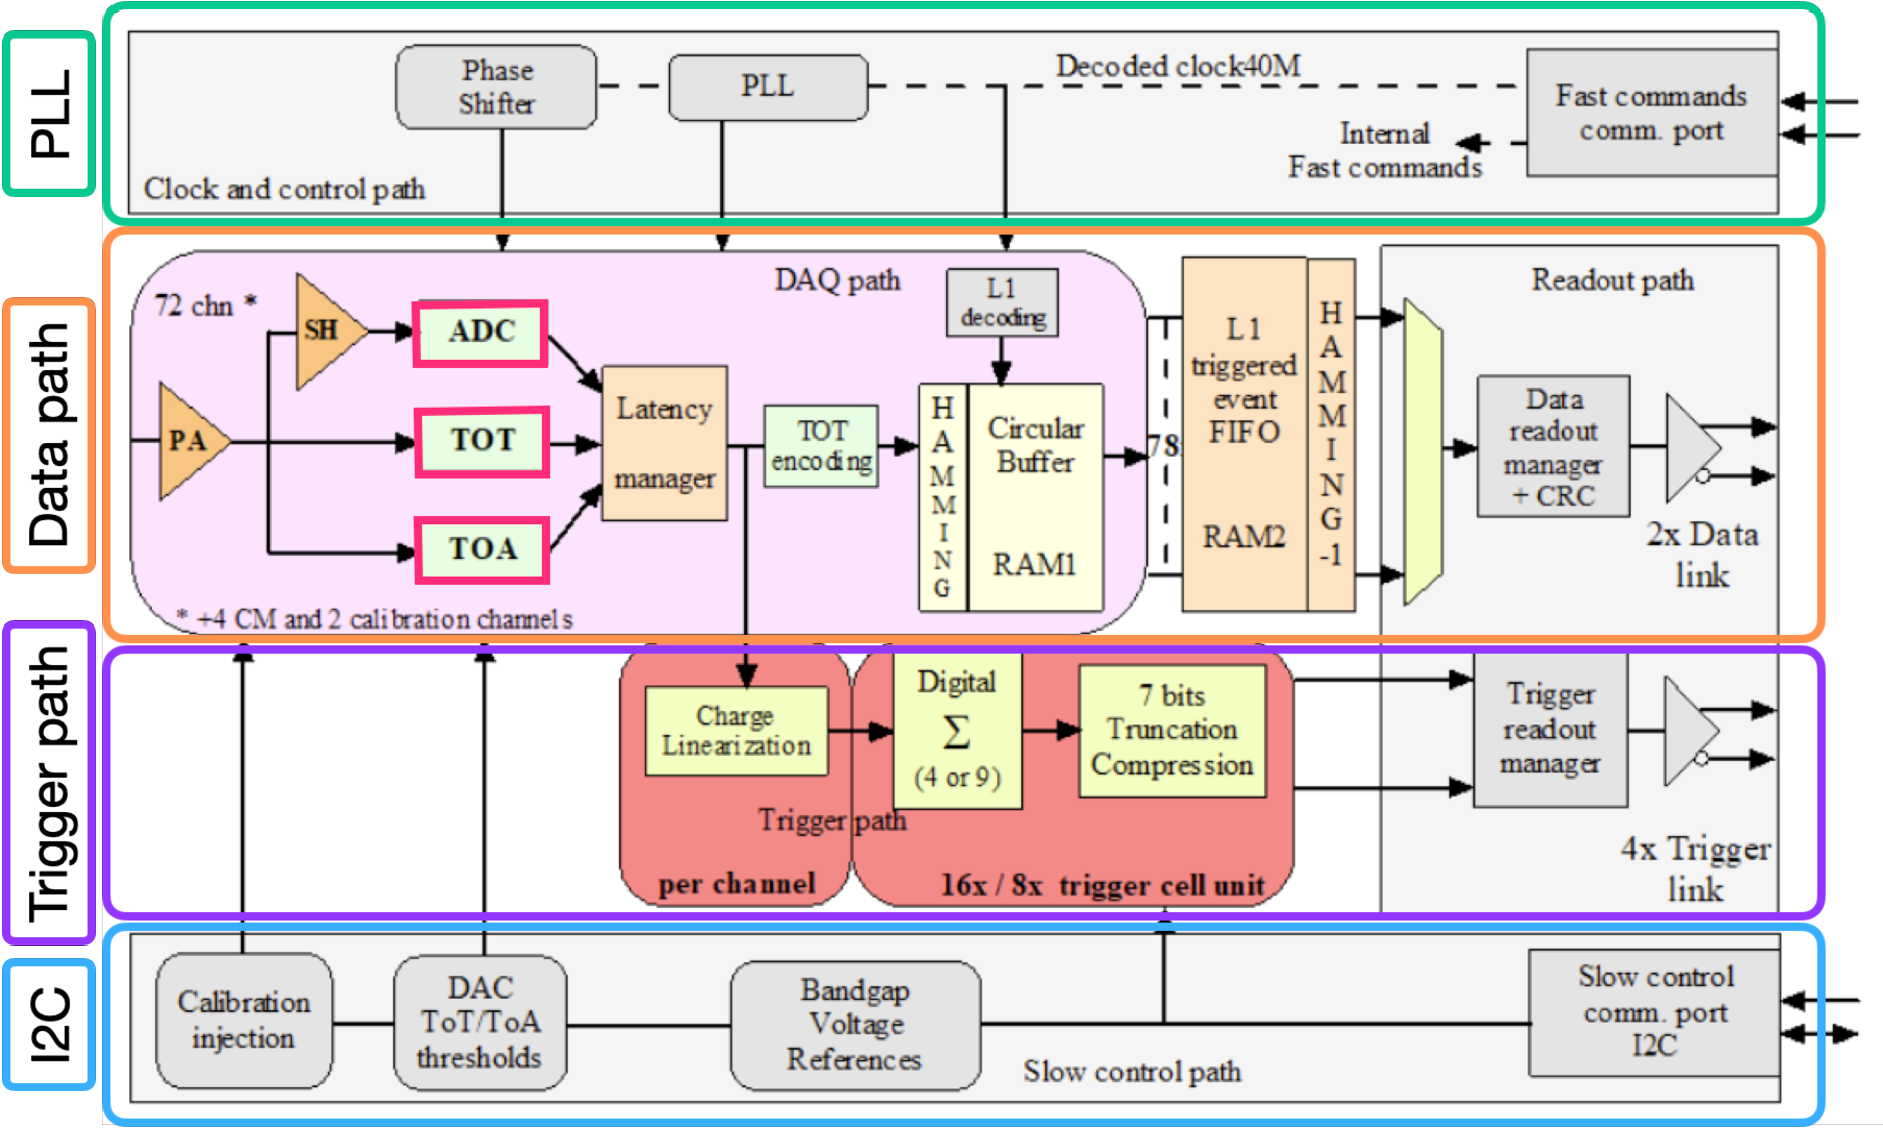
\includegraphics[width=0.75\linewidth]{Figures/HGCAL/Architecture.pdf}
    \caption{Architectural overview of the HGCROC3 read-out ASIC. The main parts composing the Data path, Trigger path, PLL and I2C have been highlighted.}
    \label{fig:Architecture}
\end{figure}

\paragraph{Data path}
The data path is the core of the chip, replicated for 72 channels of the full analog chain, 4 common mode channels for the coherent noise subtraction, and 2 calibration channels for the MIP calibration. This component extracts from the signal input charge three digitised quantities to be sent to the back-end electronics: the ADC for the charge measurement, the ToA (Time-of-Arrival) for the time measurement, and the ToT (Time-over-Threshold) for the charge measurement of saturated signals. 

The charge digitisation is achieved by a 10-bit~ADC in the linear range of the preamplifier~\cite{Firlej_2015}; when it saturates, a 12-bit Time-to-Digital Converter (TDC) with 50~ps binning over 200~ns range provides the charge information by measuring the ToT. The ToA digitisation is carried out by a similar dedicated 10-bit TDC with 25~ps binning over 25~ns range.
The low-noise preamplifier gain can be adapted to different detector regions, where the MIP energy deposit can vary depending on the sensor thickness and irradiation condition.
Under the HL-LHC conditions, certain regions of the detector may exhibit notably high occupancy rates, reaching up to 50$\%$ of fired cells per bunch crossing: it is thus important that the analog shaper drops the signal sample to less than 20$\%$ by the start of the next bunch crossing to mitigate the out-of-time pile-up.

Beyond the analog performance, the chip embeds a large part of digital processing to manage the Data and the Trigger paths. A 512-depth DRAM (RAM1) is used as a circular memory to buffer the data to accommodate the 12.5~$\mu$s latency of the L1 trigger, and a 32-depth DRAM (RAM2) is used as a FIFO after the L1 selection.
Two 1.28~Gbps links are dedicated to sending out the full event information of the selected bunch crossings after an L1 request.

\paragraph{Trigger path}
The trigger path computes an image of the deposited charge at each bunch crossing, by summing and compressing data over neighbouring channels. The two charge-related quantities from the channel information (ADC and ToT) are fed into the trigger path. The chip performs the data processing with a charge linearisation over the ADC and ToT range and computes the energy sums over 4 (9) adjacent channels for the LD (HD) modules. After compressing the information to 7 bits, it sends the trigger data to the ECON-T concentrator chip.
Four $1.28\,\textrm{Gbps}$ differential links are devoted to sending the energy sums for the L1 trigger decision.

\paragraph{PLL}
The Phase-Locked Loop (PLL) is an analog clock synthesizer receiving the 40~MHz LHC clock and providing all the other clock frequencies - from 160~MHz to 1.28~GHz - used by the circuit.
The main challenge for the PLL circuit is to ensure that all the clocks phases are aligned to the LHC 40~MHz input clock: a low noise digital Phase Frequency Detector (PFD) continuously checks for possible phase misalignments and, in case one is found, adjusts the voltage-controlled oscillator (VCO) in order to temporarily increase or decrease the frequency and realign the phase. The PLL is an essential component for the HGCROC3 functioning and has been intensively tested during the irradiation campaigns, as described in Section~\ref{sec:Single Event Effect}.

\paragraph{I2C}
The Inter-Integrated Circuit (I2C) is an internal static memory register storing the chip configuration parameters.
The I2C protocol is used to set or read the more than 7,900 parameters, distributed into 8 internal registers.
A Fast Command block is used to read and write the configuration parameters, to configure the operating mode of the system (link synchronisation, reset, calibration, L1 request, etc.), and to communicate with the device.

%%%%%%%%%%%%%%%%%%%%%%%%%%%%%%%%%%%%%%%%%%%%%%%%%%%%%%%%%%%%%%%%%%%%%%%%%%%%%%%%%%%%%%%%%%%%
%%%%%%%%%%%%%%%%%%%%%%%%%%%%%%%%%%%%%%%%%%%%%%%%%%%%%%%%%%%%%%%%%%%%%%%%%%%%%%%%%%%%%%%%%%%%
%%%%%%%%%%%%%%%%%%%%%%%%%%%%%%%%%%%%%%%%%%%%%%%%%%%%%%%%%%%%%%%%%%%%%%%%%%%%%%%%%%%%%%%%%%%%
%%%%%%%%%%%%%%%%%%%%%%%%%%%%%%%%%%%%%%%%%%%%%%%%%%%%%%%%%%%%%%%%%%%%%%%%%%%%%%%%%%%%%%%%%%%%

\section{Characterisation and testing of the HGCROC3}
\label{sec:Characterisation and testing of the HGCROC3}

% When I arrived the new  HGCROC3 had just arrived and we had to test their performance in order to check whether the met the requirements
% What are the differences between HGCROC2 and 3?

The HGCROC3 read-out chip represents the culmination of many years of R\&D and technical efforts to accommodate all the HGCAL electronics requirements in a single device. Previous versions of the chip, such as the HGCROC2, included a skeleton of the final analog and digital structures: their extensive characterisation served to solidify the knowledge of the chip functionalities and optimise the data acquisition and testing procedures.
The final design, including all the features required and implemented in the HGCROC3, was submitted in \textit{Month XXXX} and the first prototypes were received in September 2021. Preliminary results of the chip performance have been published in~\cite{Dulucq:2797658} and~\cite{Bombardi:9508012}.

The characterisation of the HGCROC3 is crucial for validating its design, ensuring expected performance within acceptable limits, and guaranteeing reliability in operations. 
Through meticulous design analysis and comprehensive testing, it is possible to identify potential issues such as power consumption irregularities, temperature sensitivities, or timing violations. This procedure ensures early detection of potential defects and allows for necessary corrections before the final submission and large-scale production, guaranteeing the reliability and robustness of the final product.

\bigbreak

This section outlines the main procedures for calibrating and testing the HGCROC3, which are essential to comprehend and evaluate its performance; it illustrates the expected response of the chip to injected charge in terms of ADC, ToA and ToT measurement; finally, it presents the results from a preliminary batch testing on approximately 200 HGCROC3 prototypes and describes the unexpected behaviour caused by design defects that have been addressed in new submission of the chip design, the HGCROC3b.

\subsection{The experimental setup}

\begin{figure}
    \centering
    \includegraphics[width=0.7\linewidth]{Figures/HGCAL/Mezzanine.pdf}
    \caption{Experimental set-up for the characterisation and testing of the HGCROC3. The mezzanine board  supports the testing of a prototype of the HGCROC3. The chip is bonded to a mezzanine, that can be mounted on a PCB (right), which is connected to a FPGA system (left) interfaced with the PC for the data acquisition.}
    \label{fig:Mezzanine}
\end{figure}

The HGCROC3 testing has been performed using various types of test benches:
\begin{itemize}
    \item \textit{Mezzanine} boards, where all the power supplies are kept separated and it is possible to check the performance in an optimistic environment, with reduced couplings to the power supplies.
    \item \textit{Socket} boards, where multiple chips can be tested in series: two versions of sockets have been produced, designated for manual or automated operations respectively.
\end{itemize}

Figure~\ref{fig:Mezzanine} shows the experimental set-up for the HGCROC3 testing, using a mezzanine board that can host only one prototype. This configuration is used for testing a small number of chips in an optimistic environment. A dedicated PCB designed to support the mezzanine is used to regulate the bias voltage and measure the power consumption in different components of the chip. The communication is controlled by a FPGA system developed at CERN, interfaced with a PC for data acquisition.

\subsection{The calibration procedure}
\label{subsec:The calibration procedure}

The HGCROC3 needs to be adaptable to a wide range of scenarios, in order to ensure consistent performance across the numerous modules and channels. The presence of potential discrepancies resulting from the chip manufacturer and the selected technology might cause fluctuations between different chips or channels belonging to the same device. As a consequence, the chip design integrates configurable parameters aimed at addressing various aspects, from the optimisation of the DC levels to the mitigation of radiation-induced damage. 

A calibration procedure is essential to find the optimal parameters and constitutes the very first operation to be performed before testing the chip. It includes the optimisation of the pedestal value for each channel, the ToA and ToT thresholds setting, and the definition of the correct phase for the signal sampling. A summary of the methodologies for the chip calibration is described in the following sections.

\subsubsection{The pedestal calibration}
\label{subsubsec:The pedestal calibration}

\begin{figure}
    \centering
    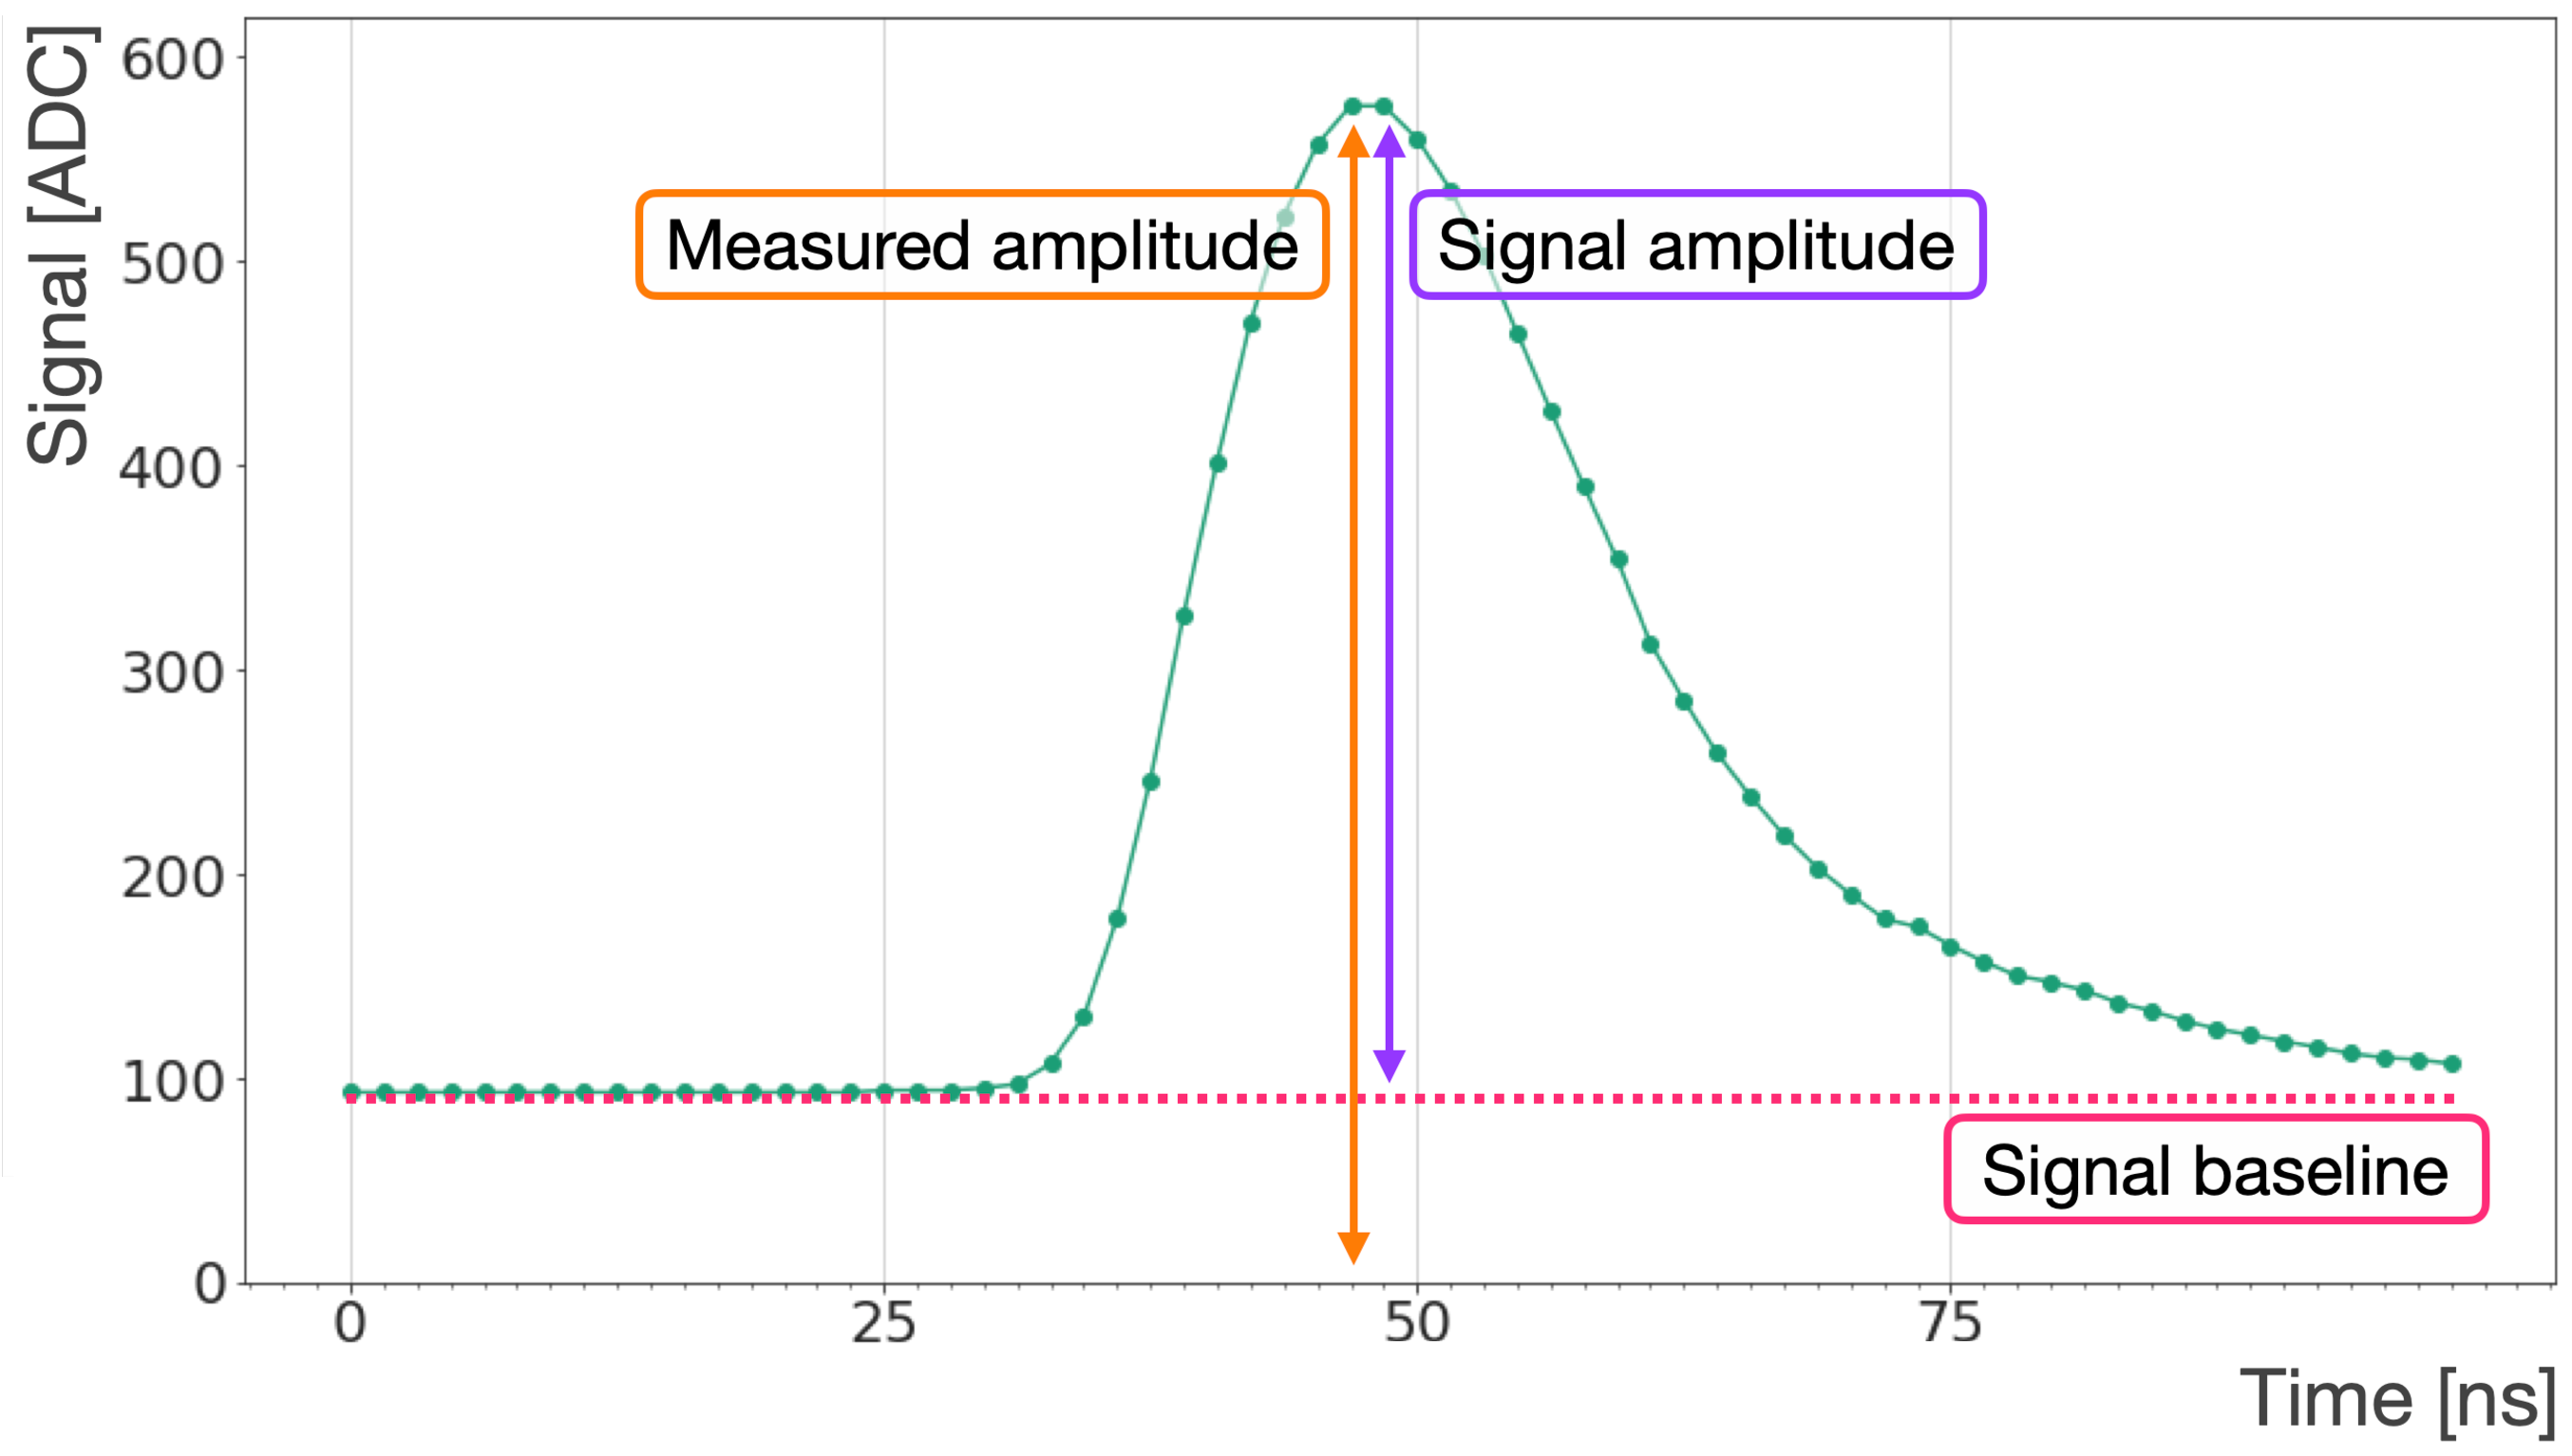
\includegraphics[width=0.6\linewidth]{Figures/HGCAL/SignalBaseline.pdf}
    \caption{A typical signal shape recorder by the HGCROC3: the pink line shows the pedestal baseline. The picture highlights the difference between the measured amplitude (orange) and the real signal amplitude (purple).}
    \label{fig:SignalBaseline}
\end{figure}

The initial step of the chip calibration procedure consists of tuning the pedestal values. The pedestal is the baseline of the signal, i.e. the ADC recorded value when no input is present. On the one hand, the pedestal value should be minimised, to fully exploit the dynamic range for the measurement of the signal amplitude. On the other hand, having a non-zero pedestal is a common practice in electronic devices to avoid a possible change in signal polarisation due to electronic noise or fluctuations of the ground potential.
Figure~\ref{fig:SignalBaseline} shows a typical signal shape recorded by the HGCROC3 with a pedestal value around 100~ADC counts. Since every signal is built on top of the baseline, it is important to know the pedestal value and subtract it from the measured amplitude to extract the real signal amplitude.

Before the calibration procedure, the 78 independent channels of the HGCROC3 present a large dispersion in their pedestal values, as shown in the left plot of Figure~\ref{fig:Pedestal}. 
A channel-wise parameter (\texttt{Trim\_Inv}) is available in the I2C register to change the pedestal of each channel independently: the parameter is coded into 6 bits, corresponding to 64 possible values.
The \textit{local} per-channel pedestal trimming is performed by scanning all possible values of the parameter and defining as a target the maximum, between all the pedestal values, for a \texttt{Trim\_Inv} value of 0. The \texttt{Trim\_Inv} of each channel will be set to the value giving a pedestal as close as possible to the target.
The full scan of the pedestal trimming value is performed separately for each half of the HGCROC3 and is shown in Figure~\ref{fig:PedestalScan}.

\begin{figure}
    \centering
    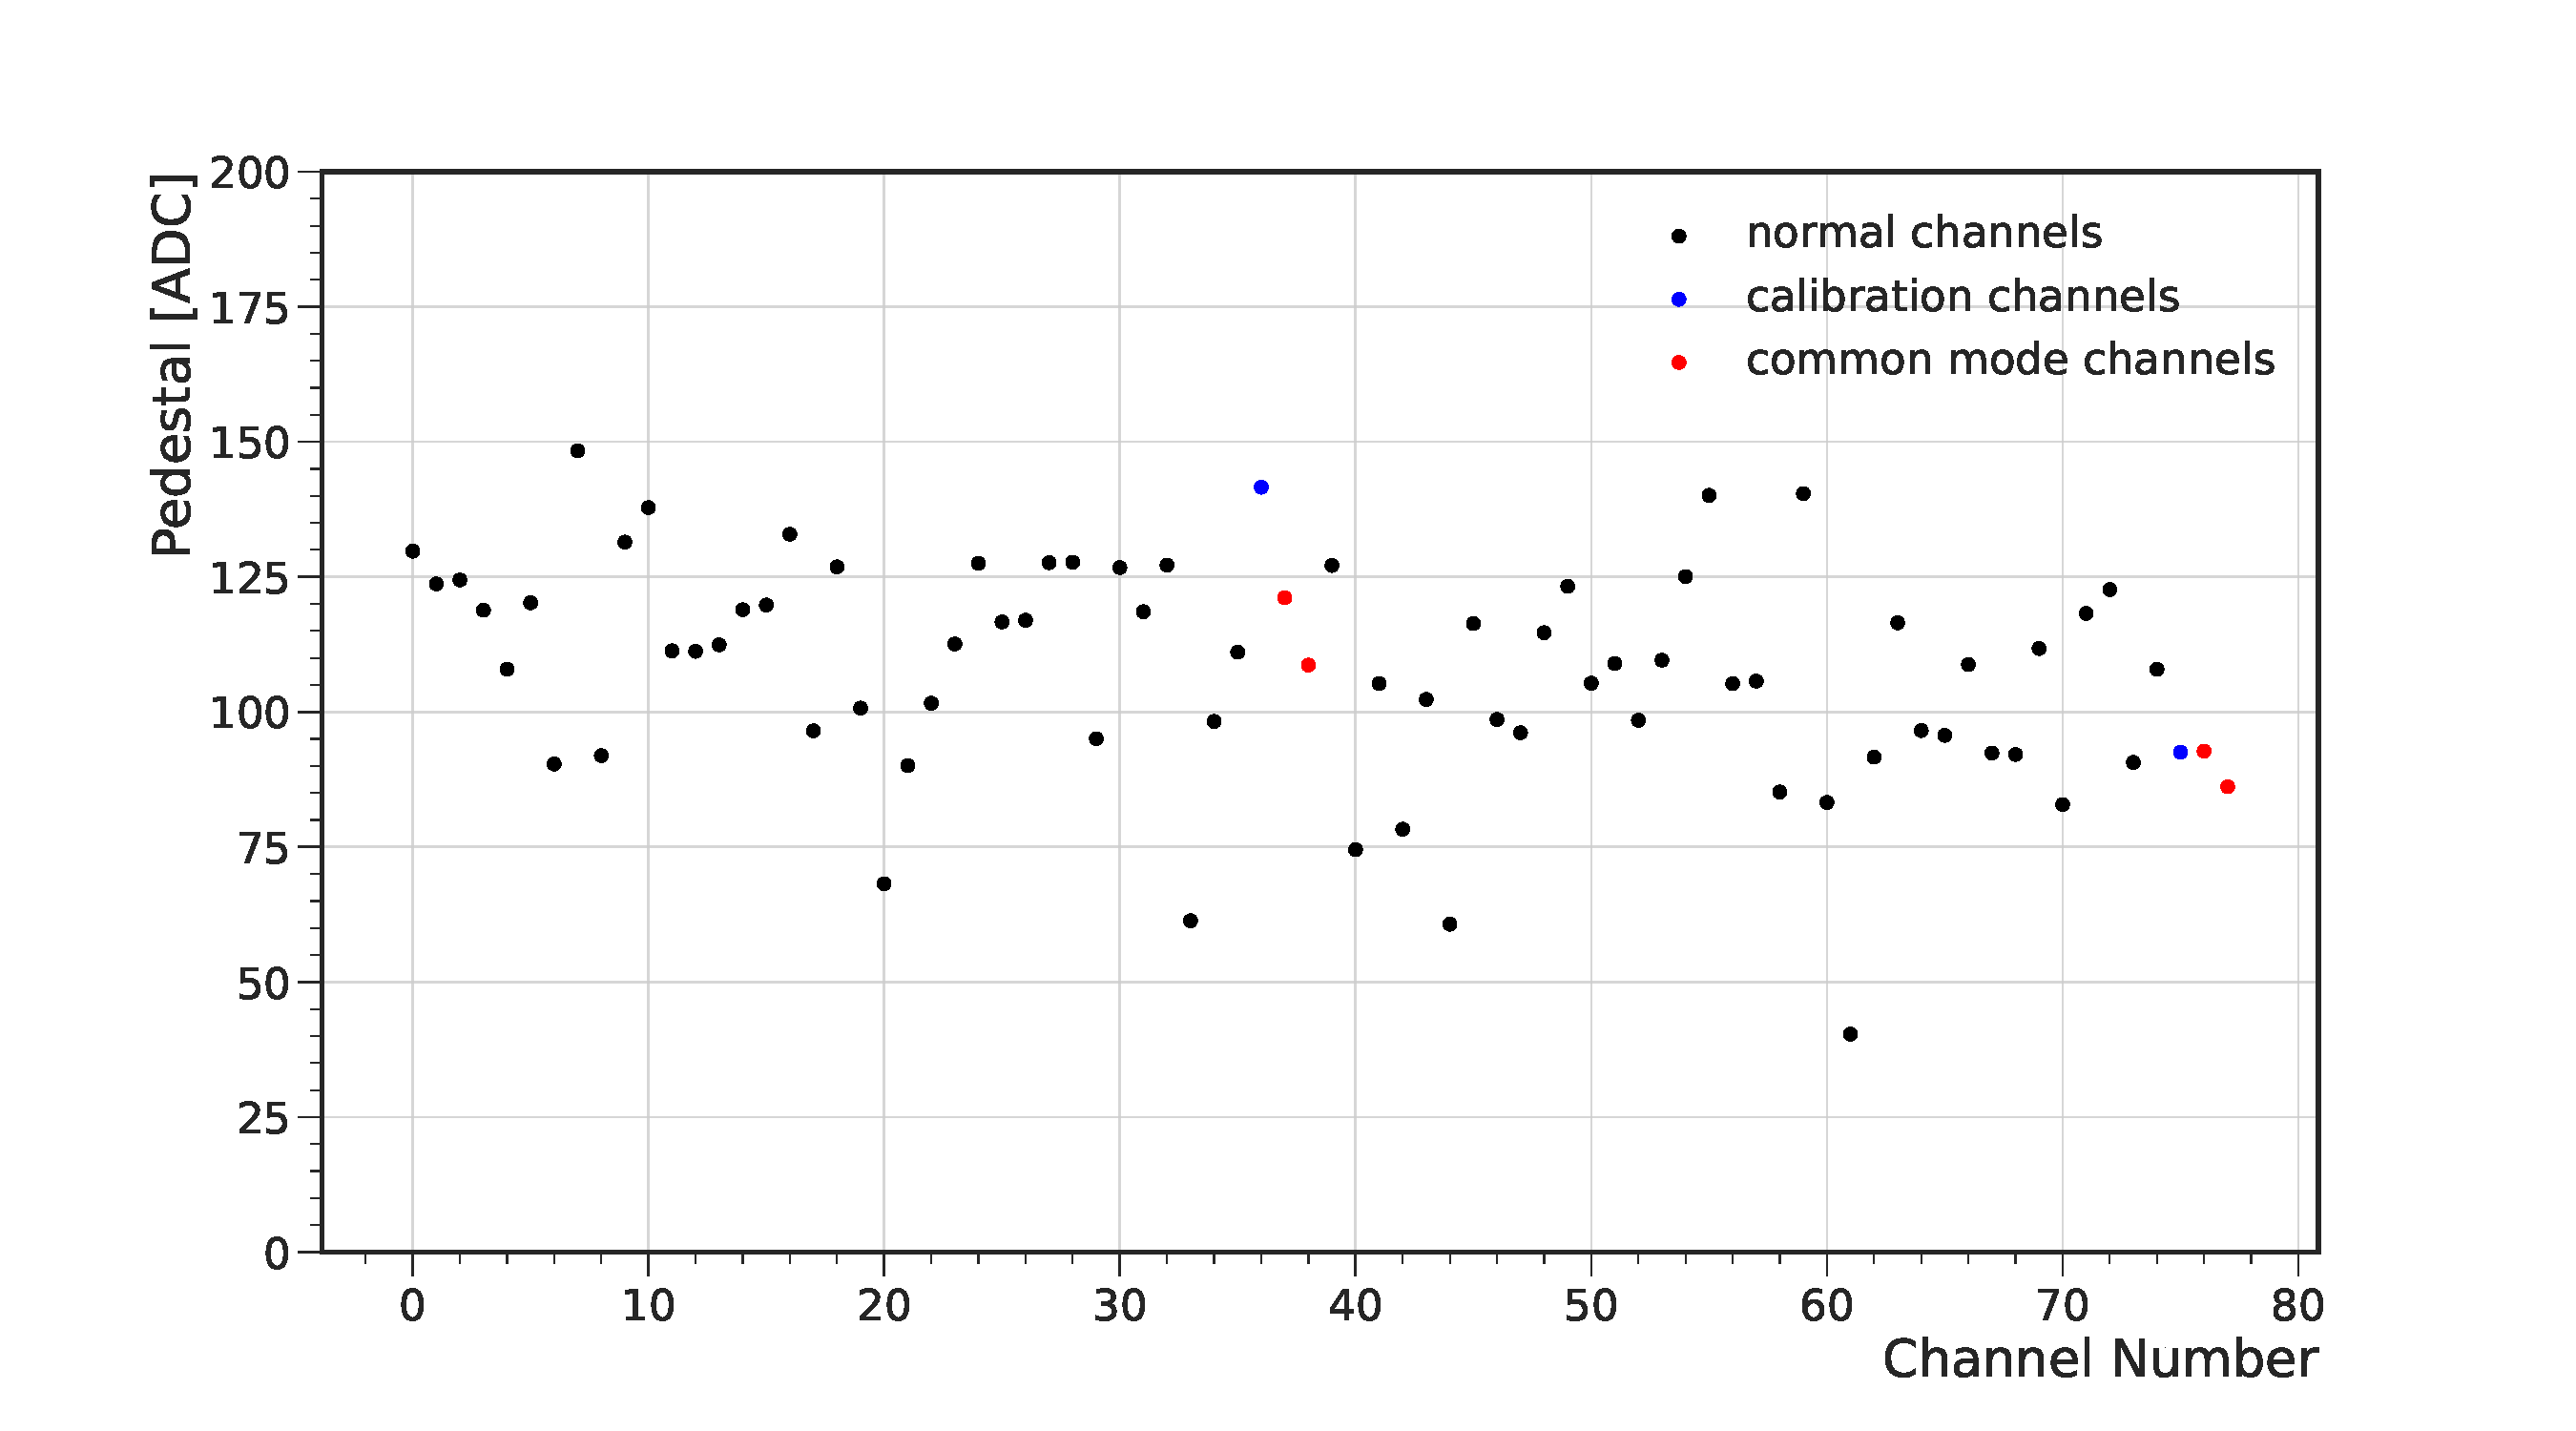
\includegraphics[width=0.49\linewidth]{Figures/HGCAL/Pedestal_Before.pdf}
    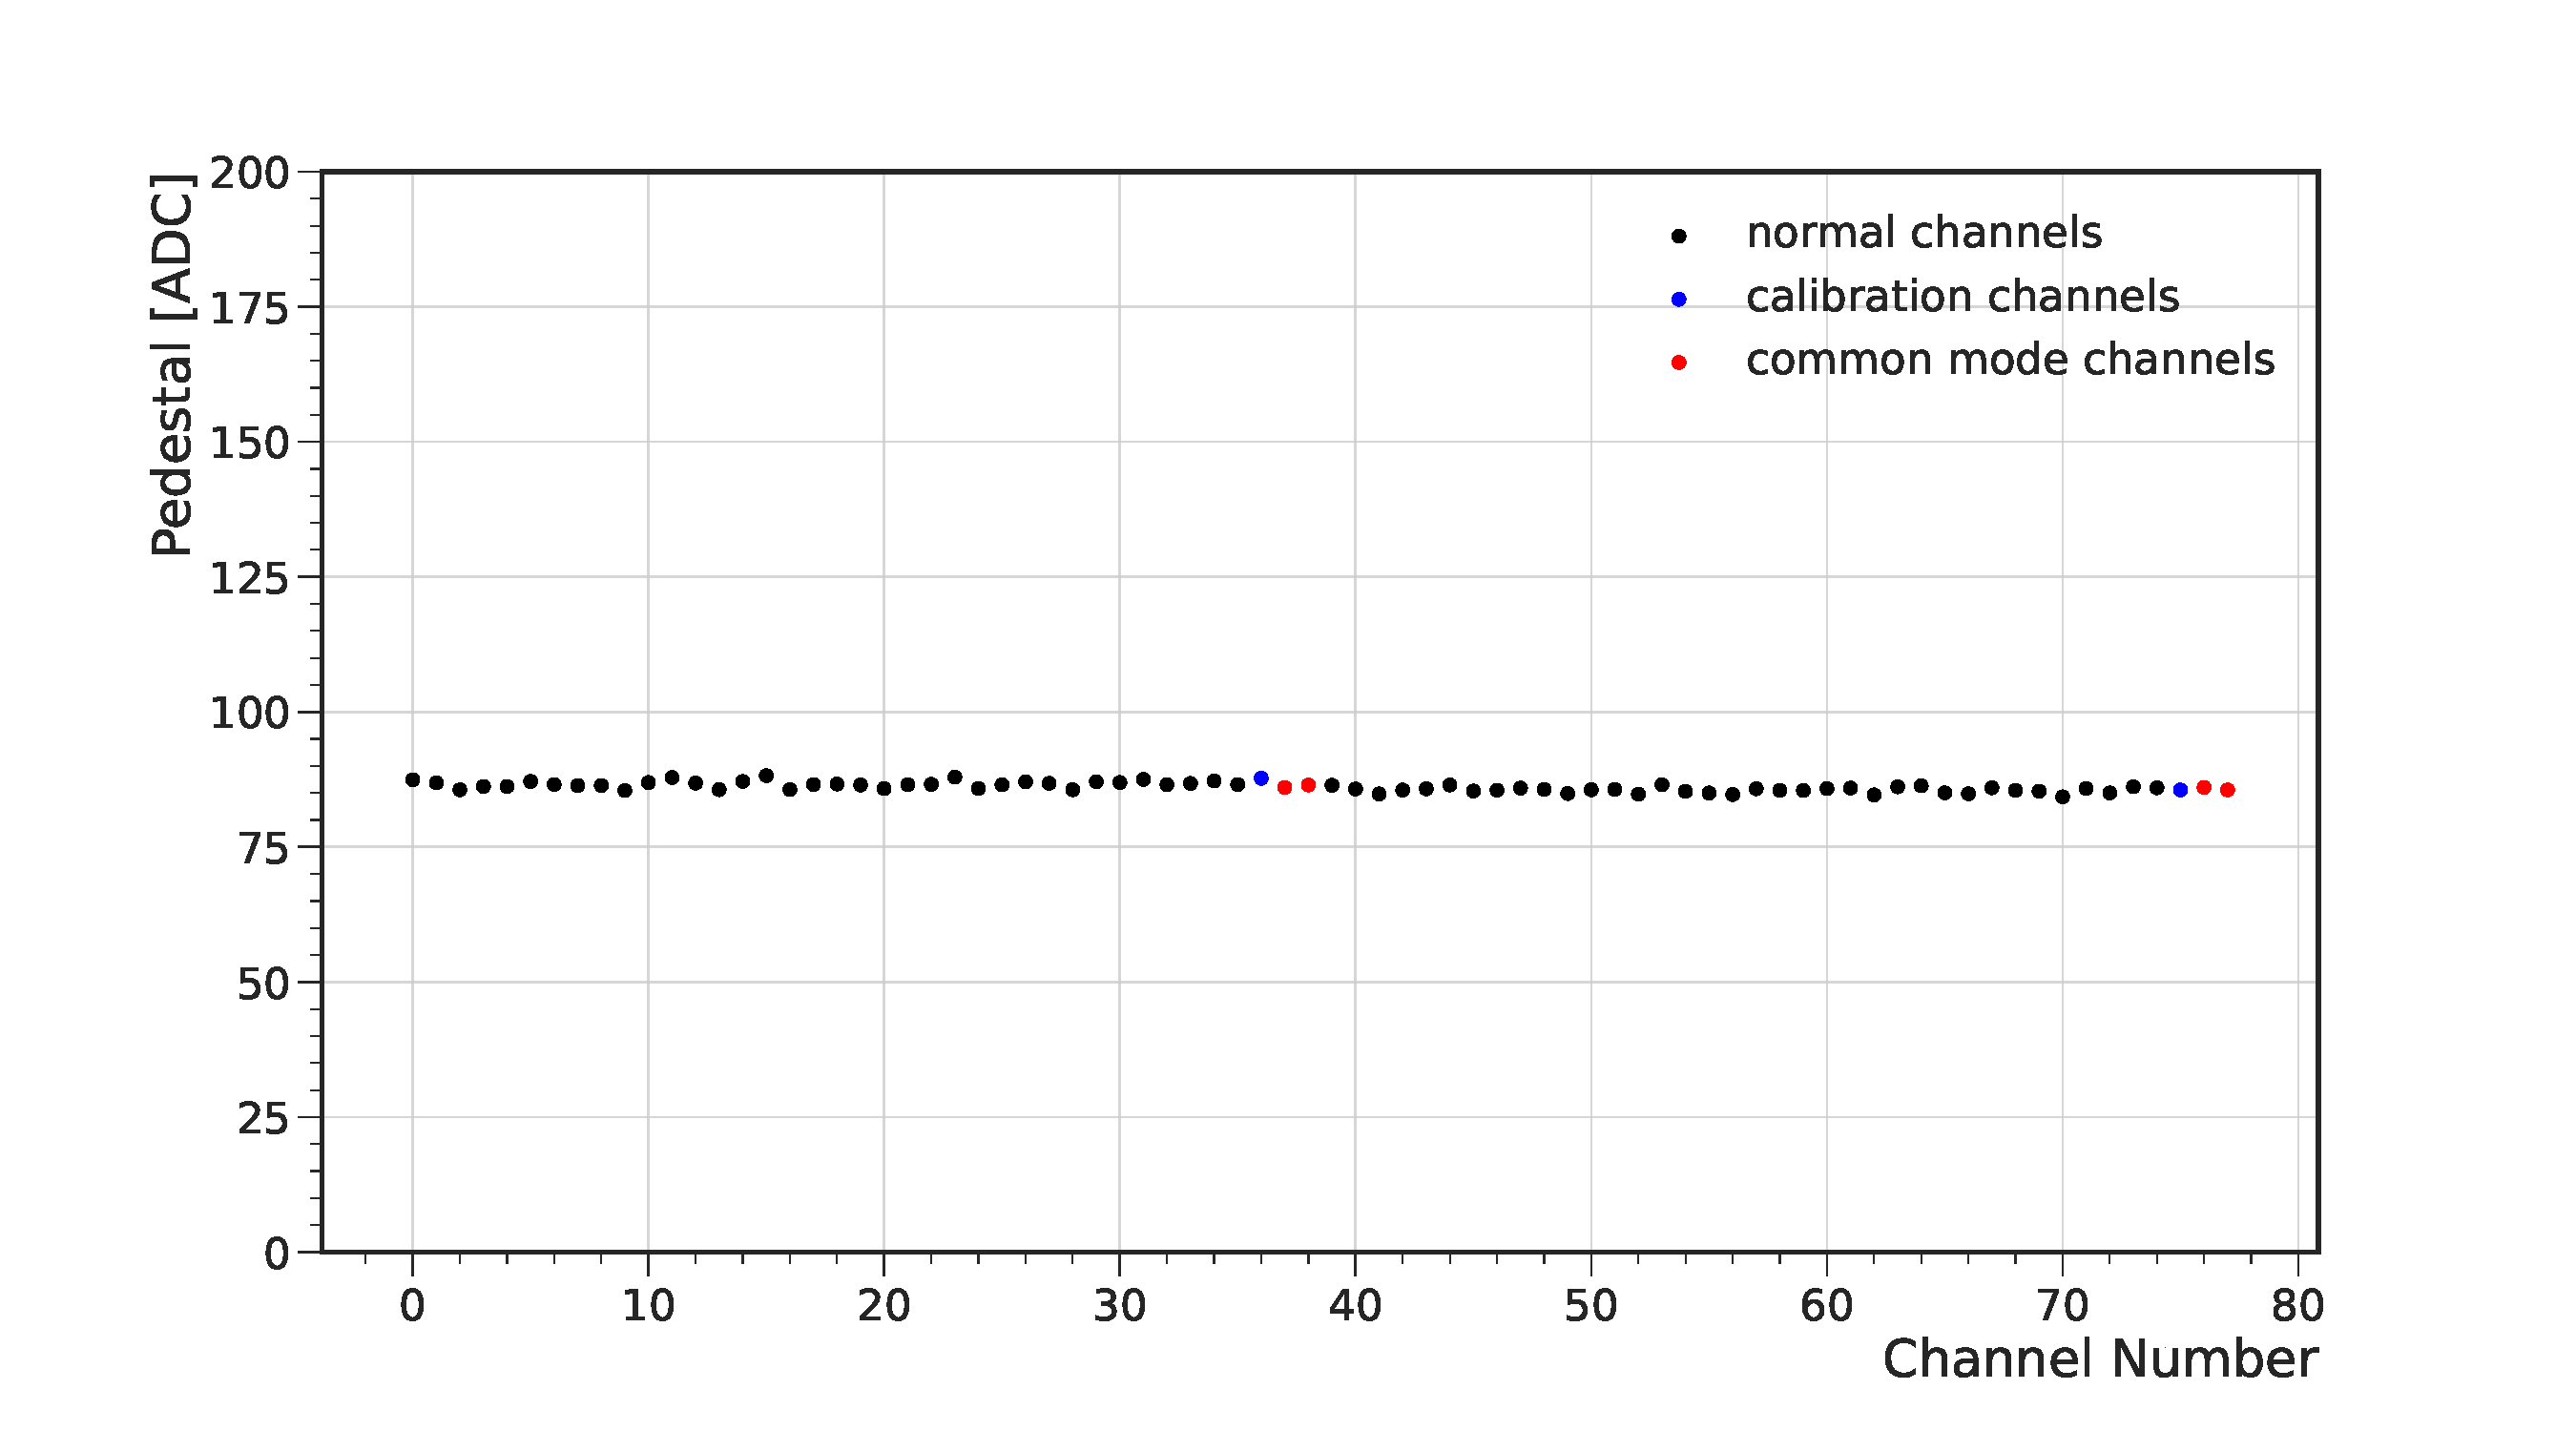
\includegraphics[width=0.49\linewidth]{Figures/HGCAL/Pedestal_After.pdf}
    \caption{Pedestal values of the HGCROC3 channels before (left) and after (right) the pedestal calibration procedure: channel numbers from 0 to 39 belong to the first half, channel numbers from 40 to 77 belong to the second half of the chip. The main target of the calibration is to reduce the dispersion between the channels and minimise their average.}
    \label{fig:Pedestal}
\end{figure}

\begin{figure} 
    \centering
    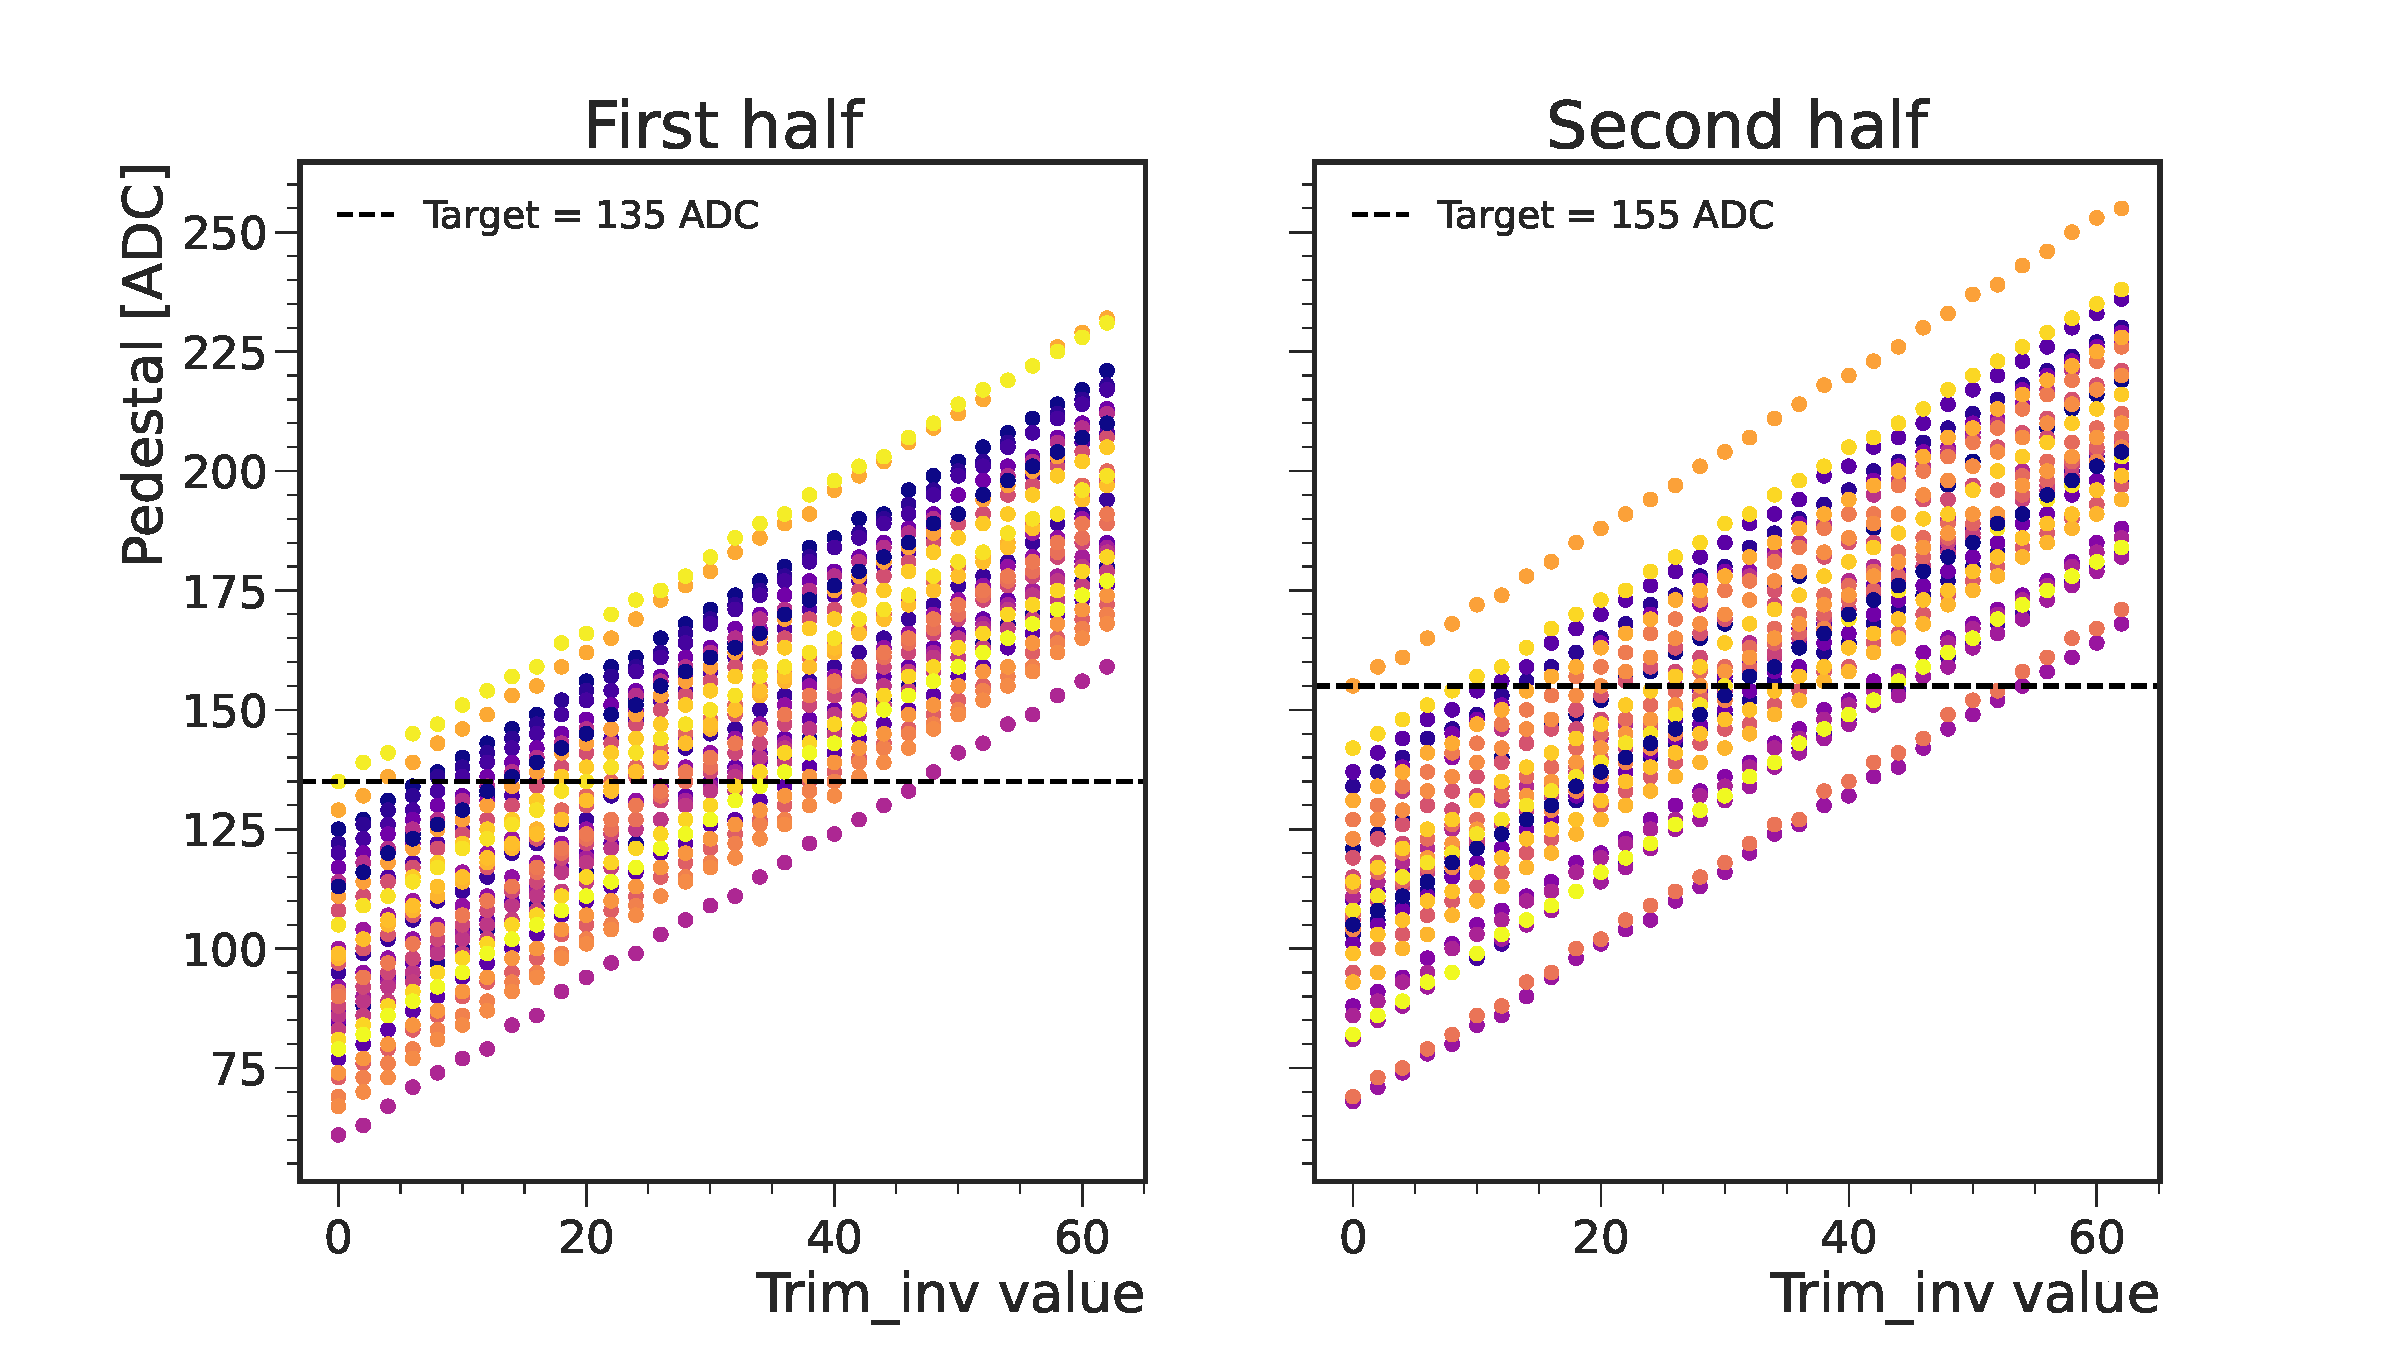
\includegraphics[width=0.7\linewidth]{Figures/HGCAL/Pedestal_Scan.pdf}
    \caption{Pedestal values of the HGCROC3 channels as a function of the \texttt{Trim\_Inv} parameter, used for a channel-wise pedestal trimming.}
    \label{fig:PedestalScan}
\end{figure}

\begin{figure}
    \centering
    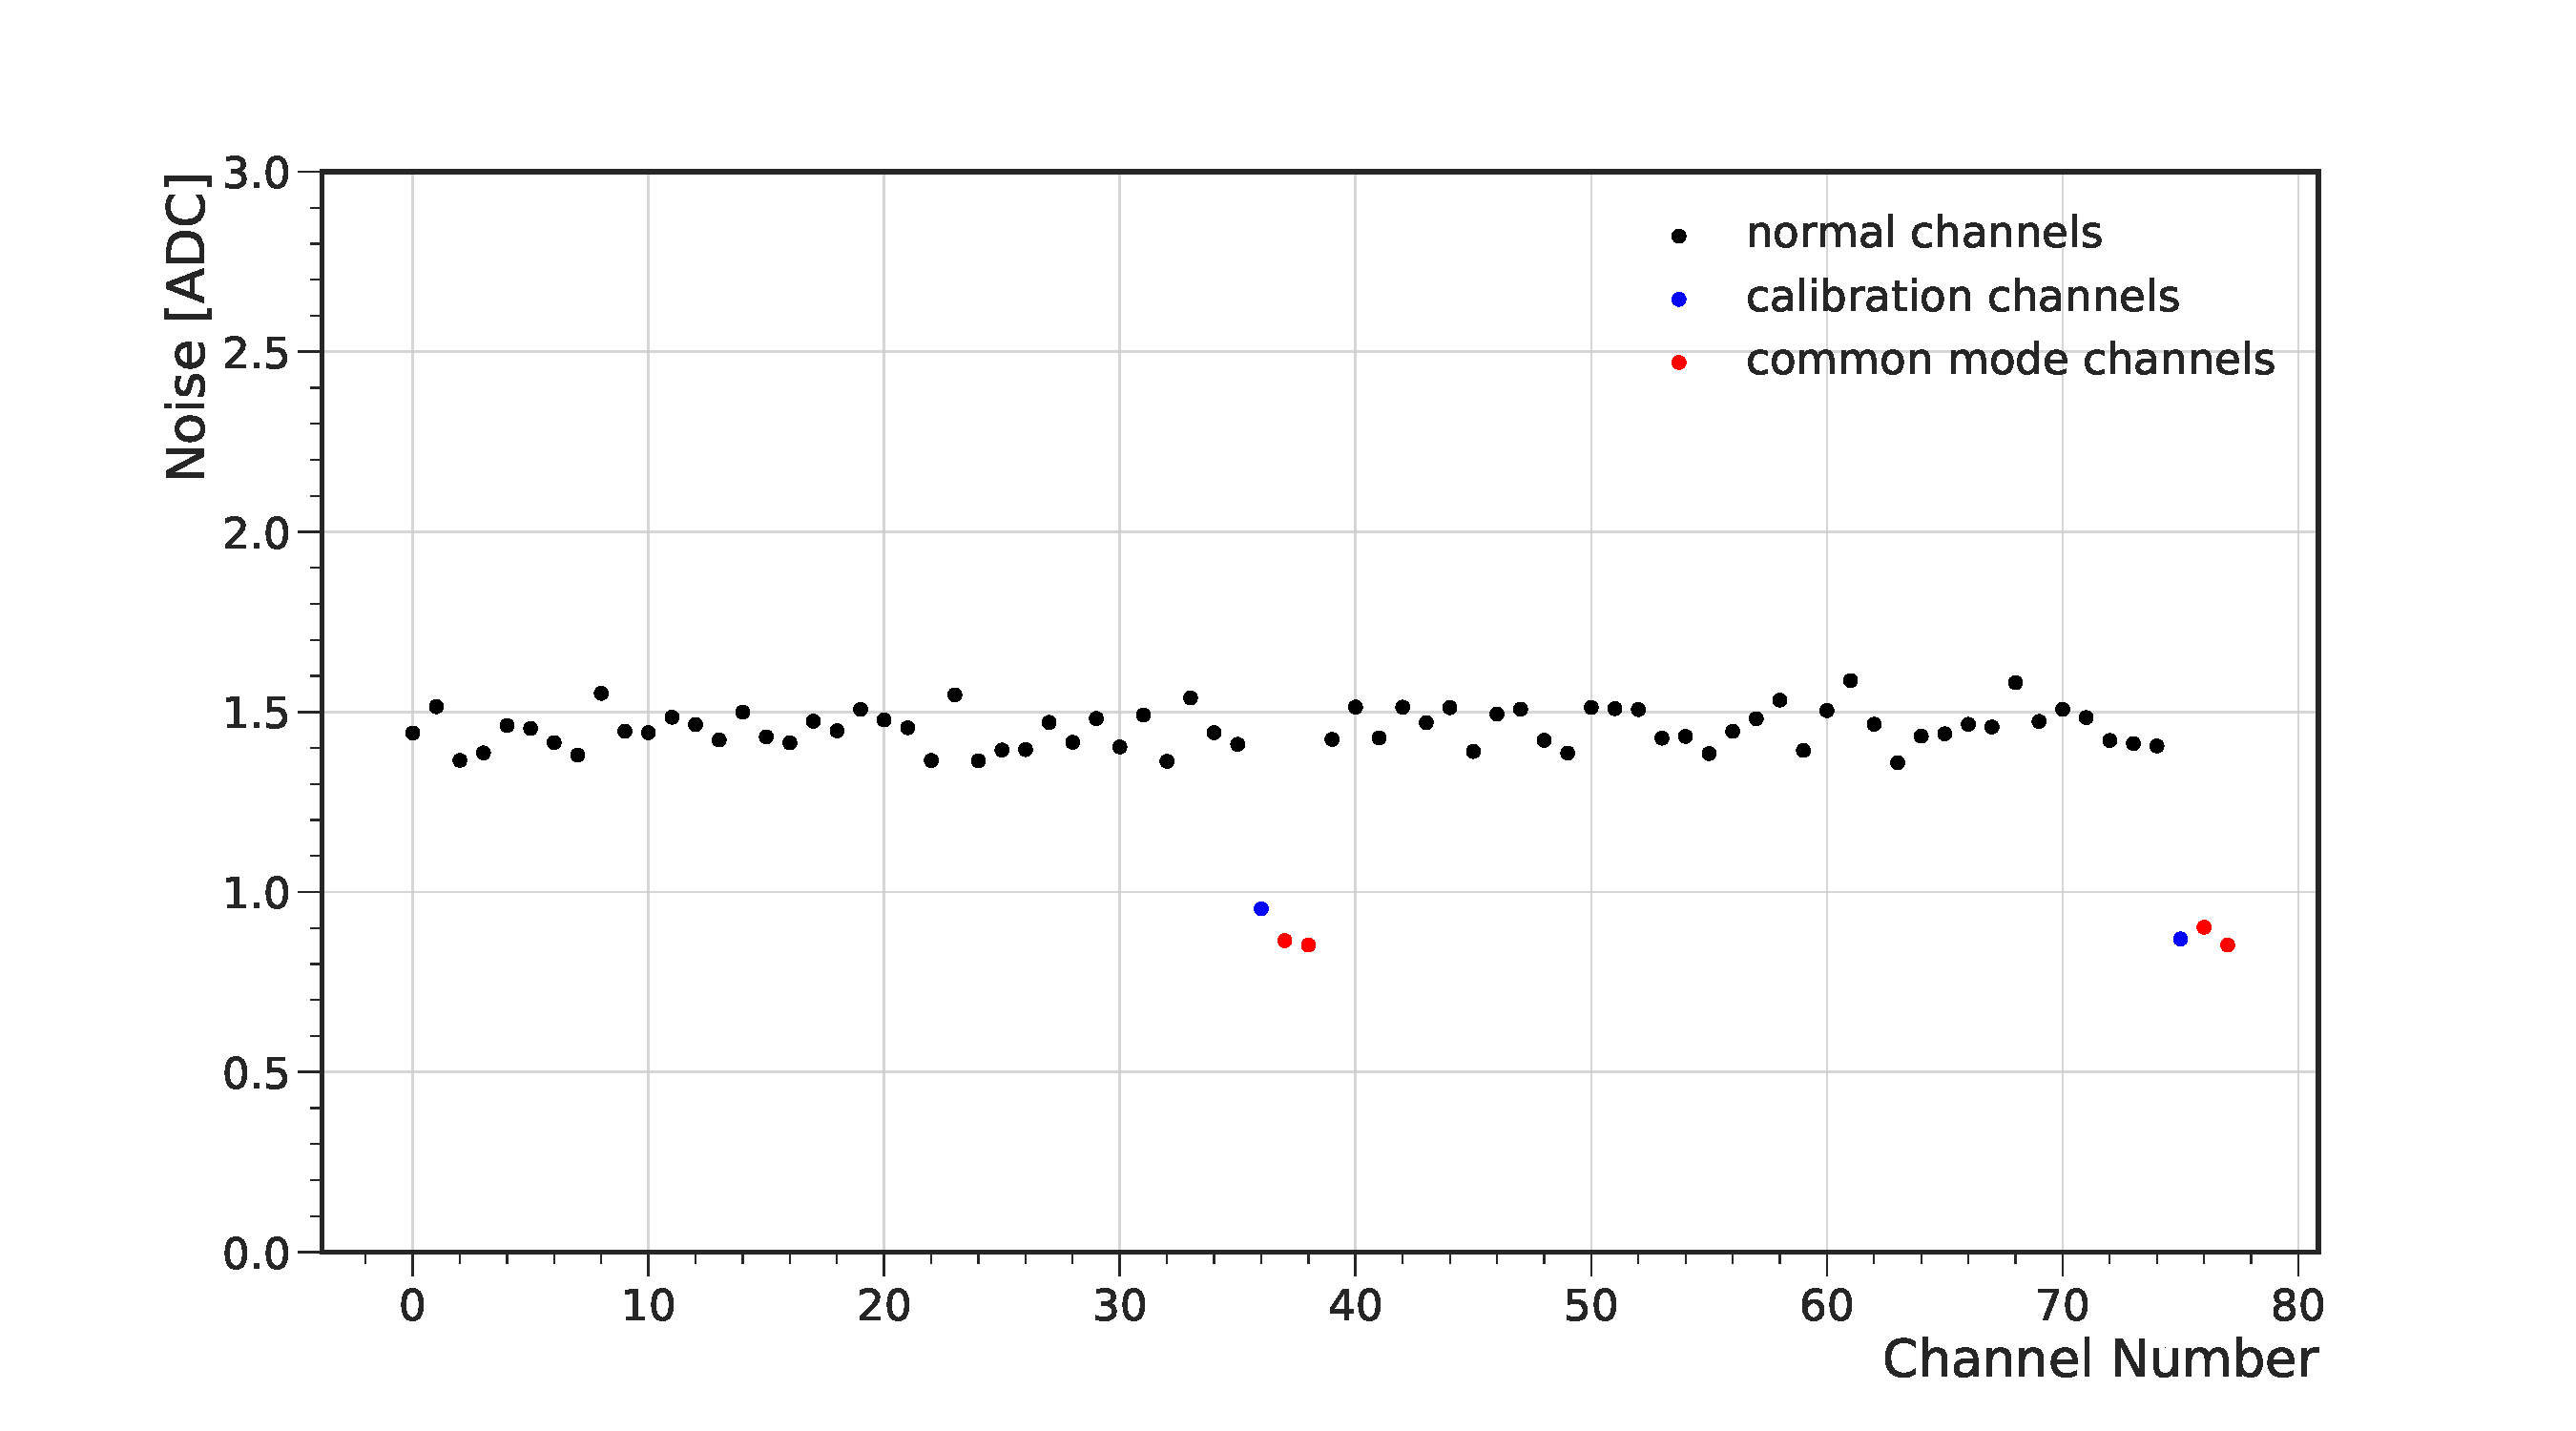
\includegraphics[width=0.55\linewidth]{Figures/HGCAL/Noise_After.pdf}
    \caption{Noise values of the HGCROC3 channels after the pedestal calibration procedure: channel numbers from 0 to 39 belong to the first half, channel numbers from 40 to 77 belong to the second half of the chip.}
    \label{fig:Noise}
\end{figure}

Once each half shows a similar pedestal value in all channels, a \textit{global} pedestal trimming is performed to lower the pedestal value to approximately 10~ADC and fully exploit the 1~V digitisation range.
The global pedestal value is configurable through two per-half parameters, \texttt{Vref\_Inv} and \texttt{Vref\_NoInv}, in such a way that the 1~V signal range is placed at the centre of the 1.2~V dynamic range of the chip.
The configuration of the pedestal value depends on the expected noise levels and ground fluctuations of the testing set-up: in the batch testing experimental conditions, high variations of the ground potential are expected, for this reason, the pedestal value is set to a slightly higher level around 50~ADC to maintain a discrete margin.

\bigbreak

The final configuration of the pedestal values for the 78 channels, after the pedestal calibration procedure is show in the right plot of Figure~\ref{fig:Pedestal}. The electronic noise of each channel before and after the pedestal calibration is also shown in Figure~\ref{fig:Noise}.

% Since the analog part of the HGCROC3 is powered at 1.2~V, two per-half parameters are present in the I2C register to place the signal range at the center of the dynamic range.
% In order to better understand this procedure, it is useful to go a bit in the details of the ADC chain. Before the preamplified analog signal enters the ADC block, it is split in two signals with same shape and opposite polarisation: the positively polarised signal enters the \textit{Non Inverted} chain, while the negatively polarised signal enters the \textit{Inverted} chain. Both chains have a 1.2~V dynamic range.
% It is possible to change the values of Vref_inv and Vref_noinv in 10b-DACs (1024 values) to find the best combination. The principle is to force one of the ADC input to 0.6 V (half of the signal range), perform a scan of the Vref DAC of the other branch and set it to the value giving the code 256 ADC (266 in fact to have some margin), and then redo the same operation but for the other branch. By construction, this procedure allows the optimization of both the pedestal and the dynamic range. 

\subsubsection{The time thresholds calibration}
\label{subsubsec:The time thresholds calibration}

\begin{figure}
    \centering
    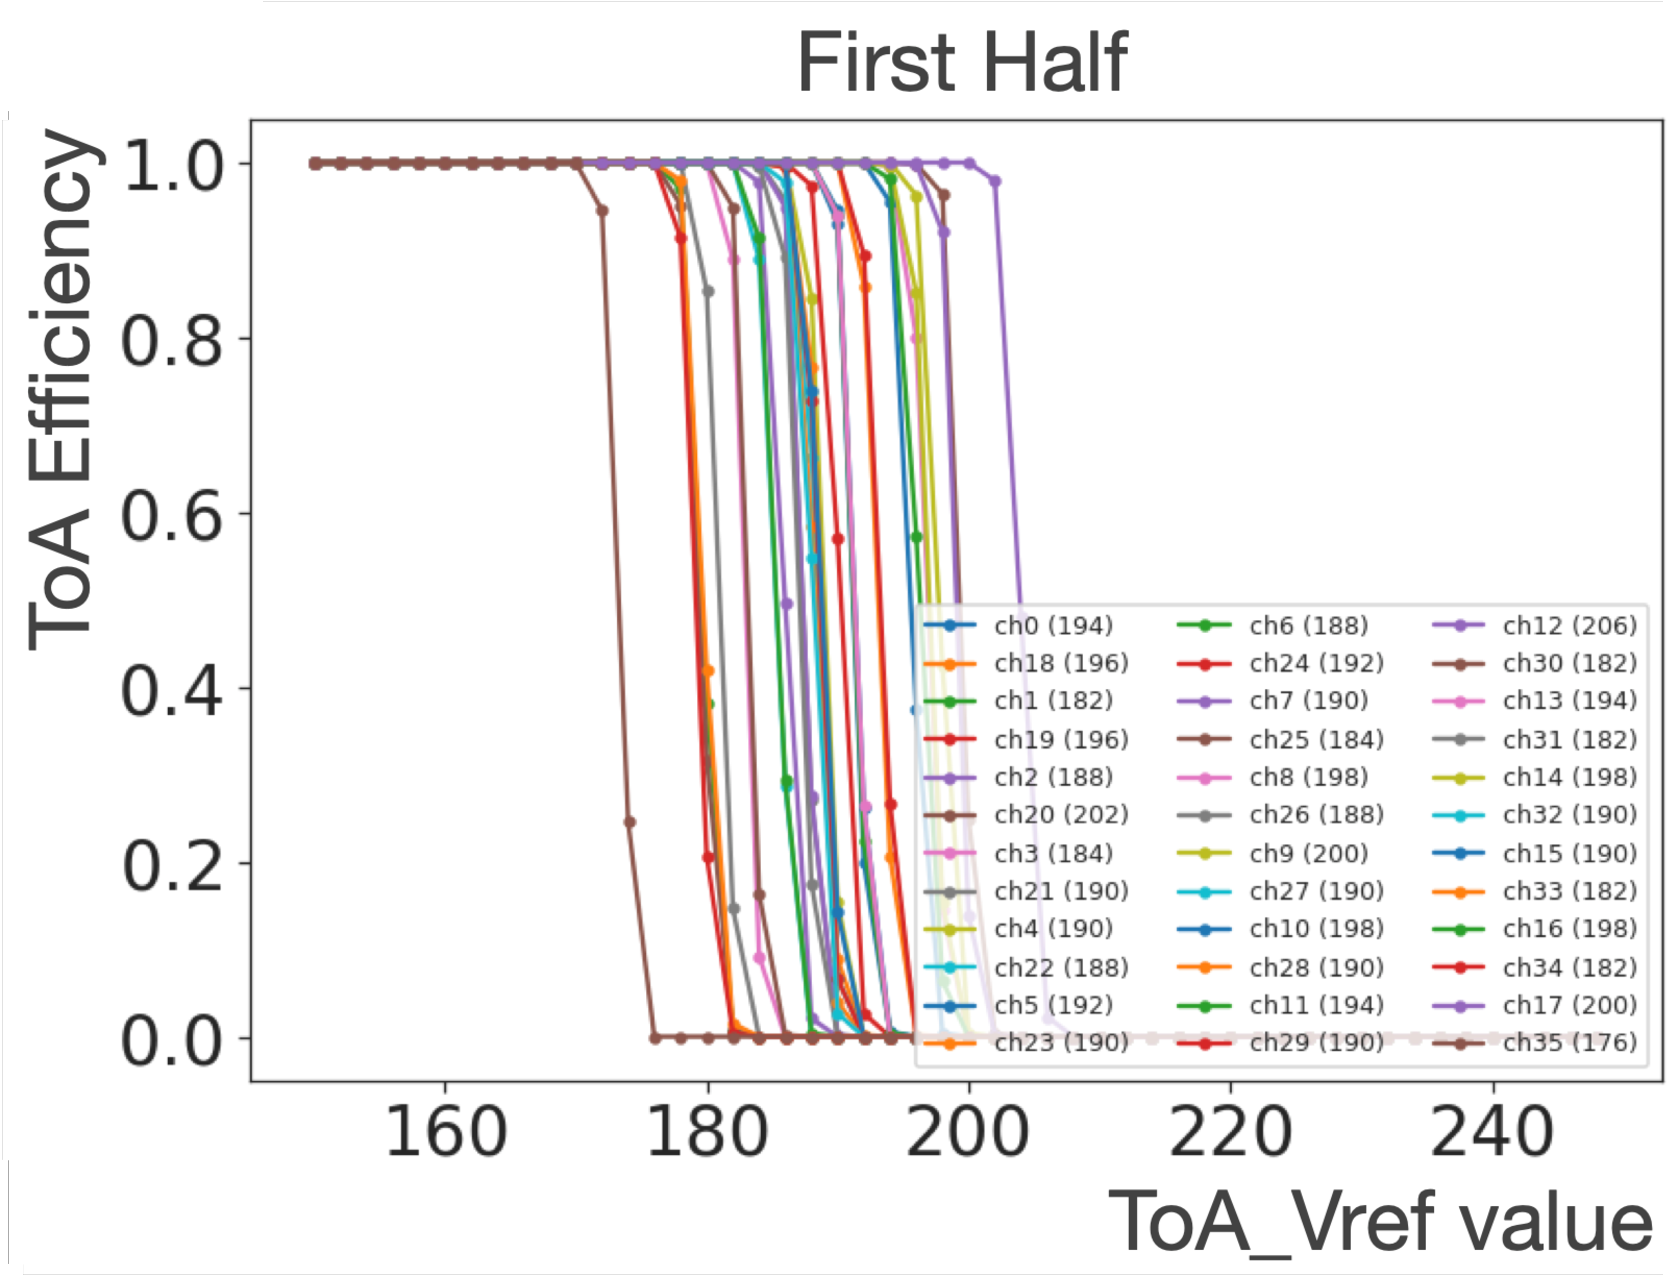
\includegraphics[width=0.49\linewidth]{Figures/HGCAL/ToA_Eff_0.pdf}
    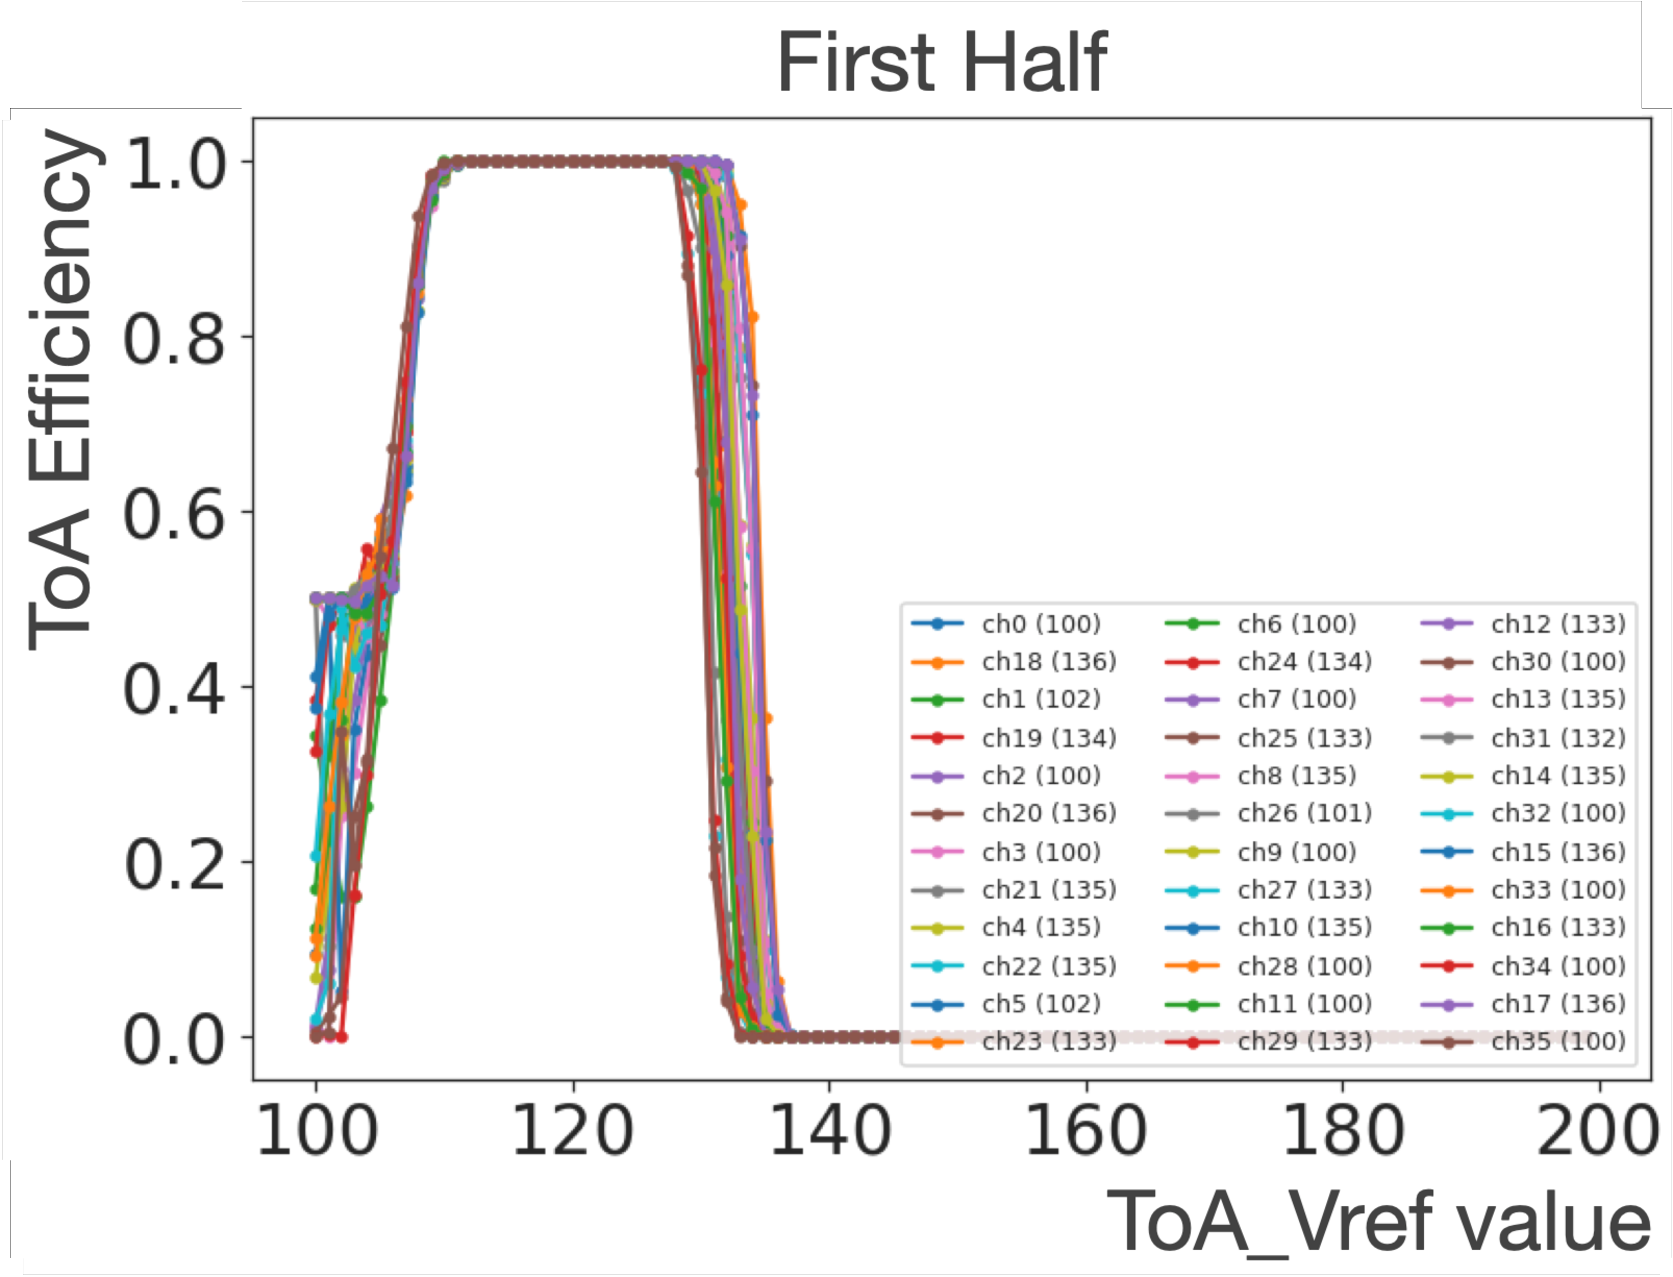
\includegraphics[width=0.49\linewidth]{Figures/HGCAL/ToA_Eff_1.pdf}
    \caption{ToA efficiency, defined as the ratio between ToA triggered events and total number of injected events, as a function of the \texttt{ToA\_Vref} parameter, defining the ToA discriminator threshold, before (left) and after (right) the ToA threshold calibration procedure.}
    \label{fig:ToAEff}
\end{figure}

The Time-of-Arrival (ToA) denotes the timing measurement of the signal, determined by the moment when the signal amplitude surpasses a predefined threshold value. The ToA threshold should be calibrated slightly above the pedestal level to ensure accurate timing acquisition for the majority of the events. Moreover, the read-out chip should provide the same timing efficiency across different modules and channels, without being affected by fluctuations in the pedestal or noise values.
In the HGCROC3, two channel-wise parameters (\texttt{ToA\_Vref} and \texttt{Trim\_ToA}) are available to calibrate the ToA thresholds in order to minimise the ToA efficiency dispersion among channels.
For the ToA calibration, a small charge with a fixed ADC amplitude is internally injected into each channel and a scan of different discriminator thresholds is performed. For each threshold, the ToA efficiency is computed, defined as the ratio of ToA triggers to the total number of injected events:
\begin{equation}
    \textnormal{ToA Efficiency} = \frac{\# \textnormal{ToA Triggered Events}}{\# \textnormal{Total Events}}
\end{equation}

If the threshold is low, all events will trigger a ToA signal and the efficiency will be equal to 1, while if the threshold is high, no event will reach the discriminator and the efficiency will be 0.
The ToA efficiency as a function of the different threshold values is presented in the left plot of Figure~\ref{fig:ToAEff} before the calibration procedure.
The goal of the ToA threshold calibration is to have, for a given \texttt{ToA\_Vref} value, the same ToA efficiency in all channels. 
Since the value of the discriminator threshold is defined as the difference between \texttt{ToA\_Vref} and \texttt{Trim\_ToA}, it is possible to configure the channel-wise \texttt{Trim\_ToA} so that the the 50$\%$ efficiency is reached for the same \texttt{ToA\_Vref} value for all channels: the final performance after the calibration procedure is shown in the right plot of Figure~\ref{fig:ToAEff}.

\bigbreak

The Time-over-Threshold (ToT) is a method to estimate the signal amplitude for very high pulses that saturate the ADC dynamic range by measuring the duration of the signal pulse saturation. 
The ToT is computed only for pulses exceeding the ToT threshold, which needs to be configured below the preamplifier saturation point, in order not to have gaps between the ADC and the ToT dynamic range of measurements. The process of establishing the ToT threshold voltage is similar to the ToA calibration method and is configurable through equivalent channel-wise parameters, \texttt{ToT\_Vref} and \texttt{Trim\_ToT}.

% The ToA injection scan measures the time of arrival of the signal. The ToA is the instant of time at which the signal amplitude exceeds a threshold value. You can see from the example that a smaller signal amplitude provides a bigger ToA, while a higher signal amplitude leads to a smaller ToA. This is reflected in the right plot, where we can see the so-called “time walk”.

\subsubsection{The phase calibration}
\label{subsubsec:The phase calibration}

To correctly measure the amplitude of the physical signal, the ADC and TDC conversion blocks of the HGCROC3 are provided with an adjustable sampling phase parameter.
Each 25~ns bunch crossing (BX) period is internally sampled into 16 phases: each ASIC can be configured in such a way that the signal amplitude is sampled at the correct phase, which might depend on the rapidity angle of the module and the silicon sensor thickness.

Figure~\ref{fig:BestPhase} shows a scan over phases of the ADC value, reconstructing the signal shape of an injected pulse: in this case, the sampling phase corresponding to the signal peak is determined to be phase 0.
The signal sampling also shows an oscillation in the pedestal value, due to the fluctuation of the ground potential.
% , that can be subtracted through the common mode channels.
%  check with Glen, CM channels used for HV noise and others

\begin{figure}
    \centering
    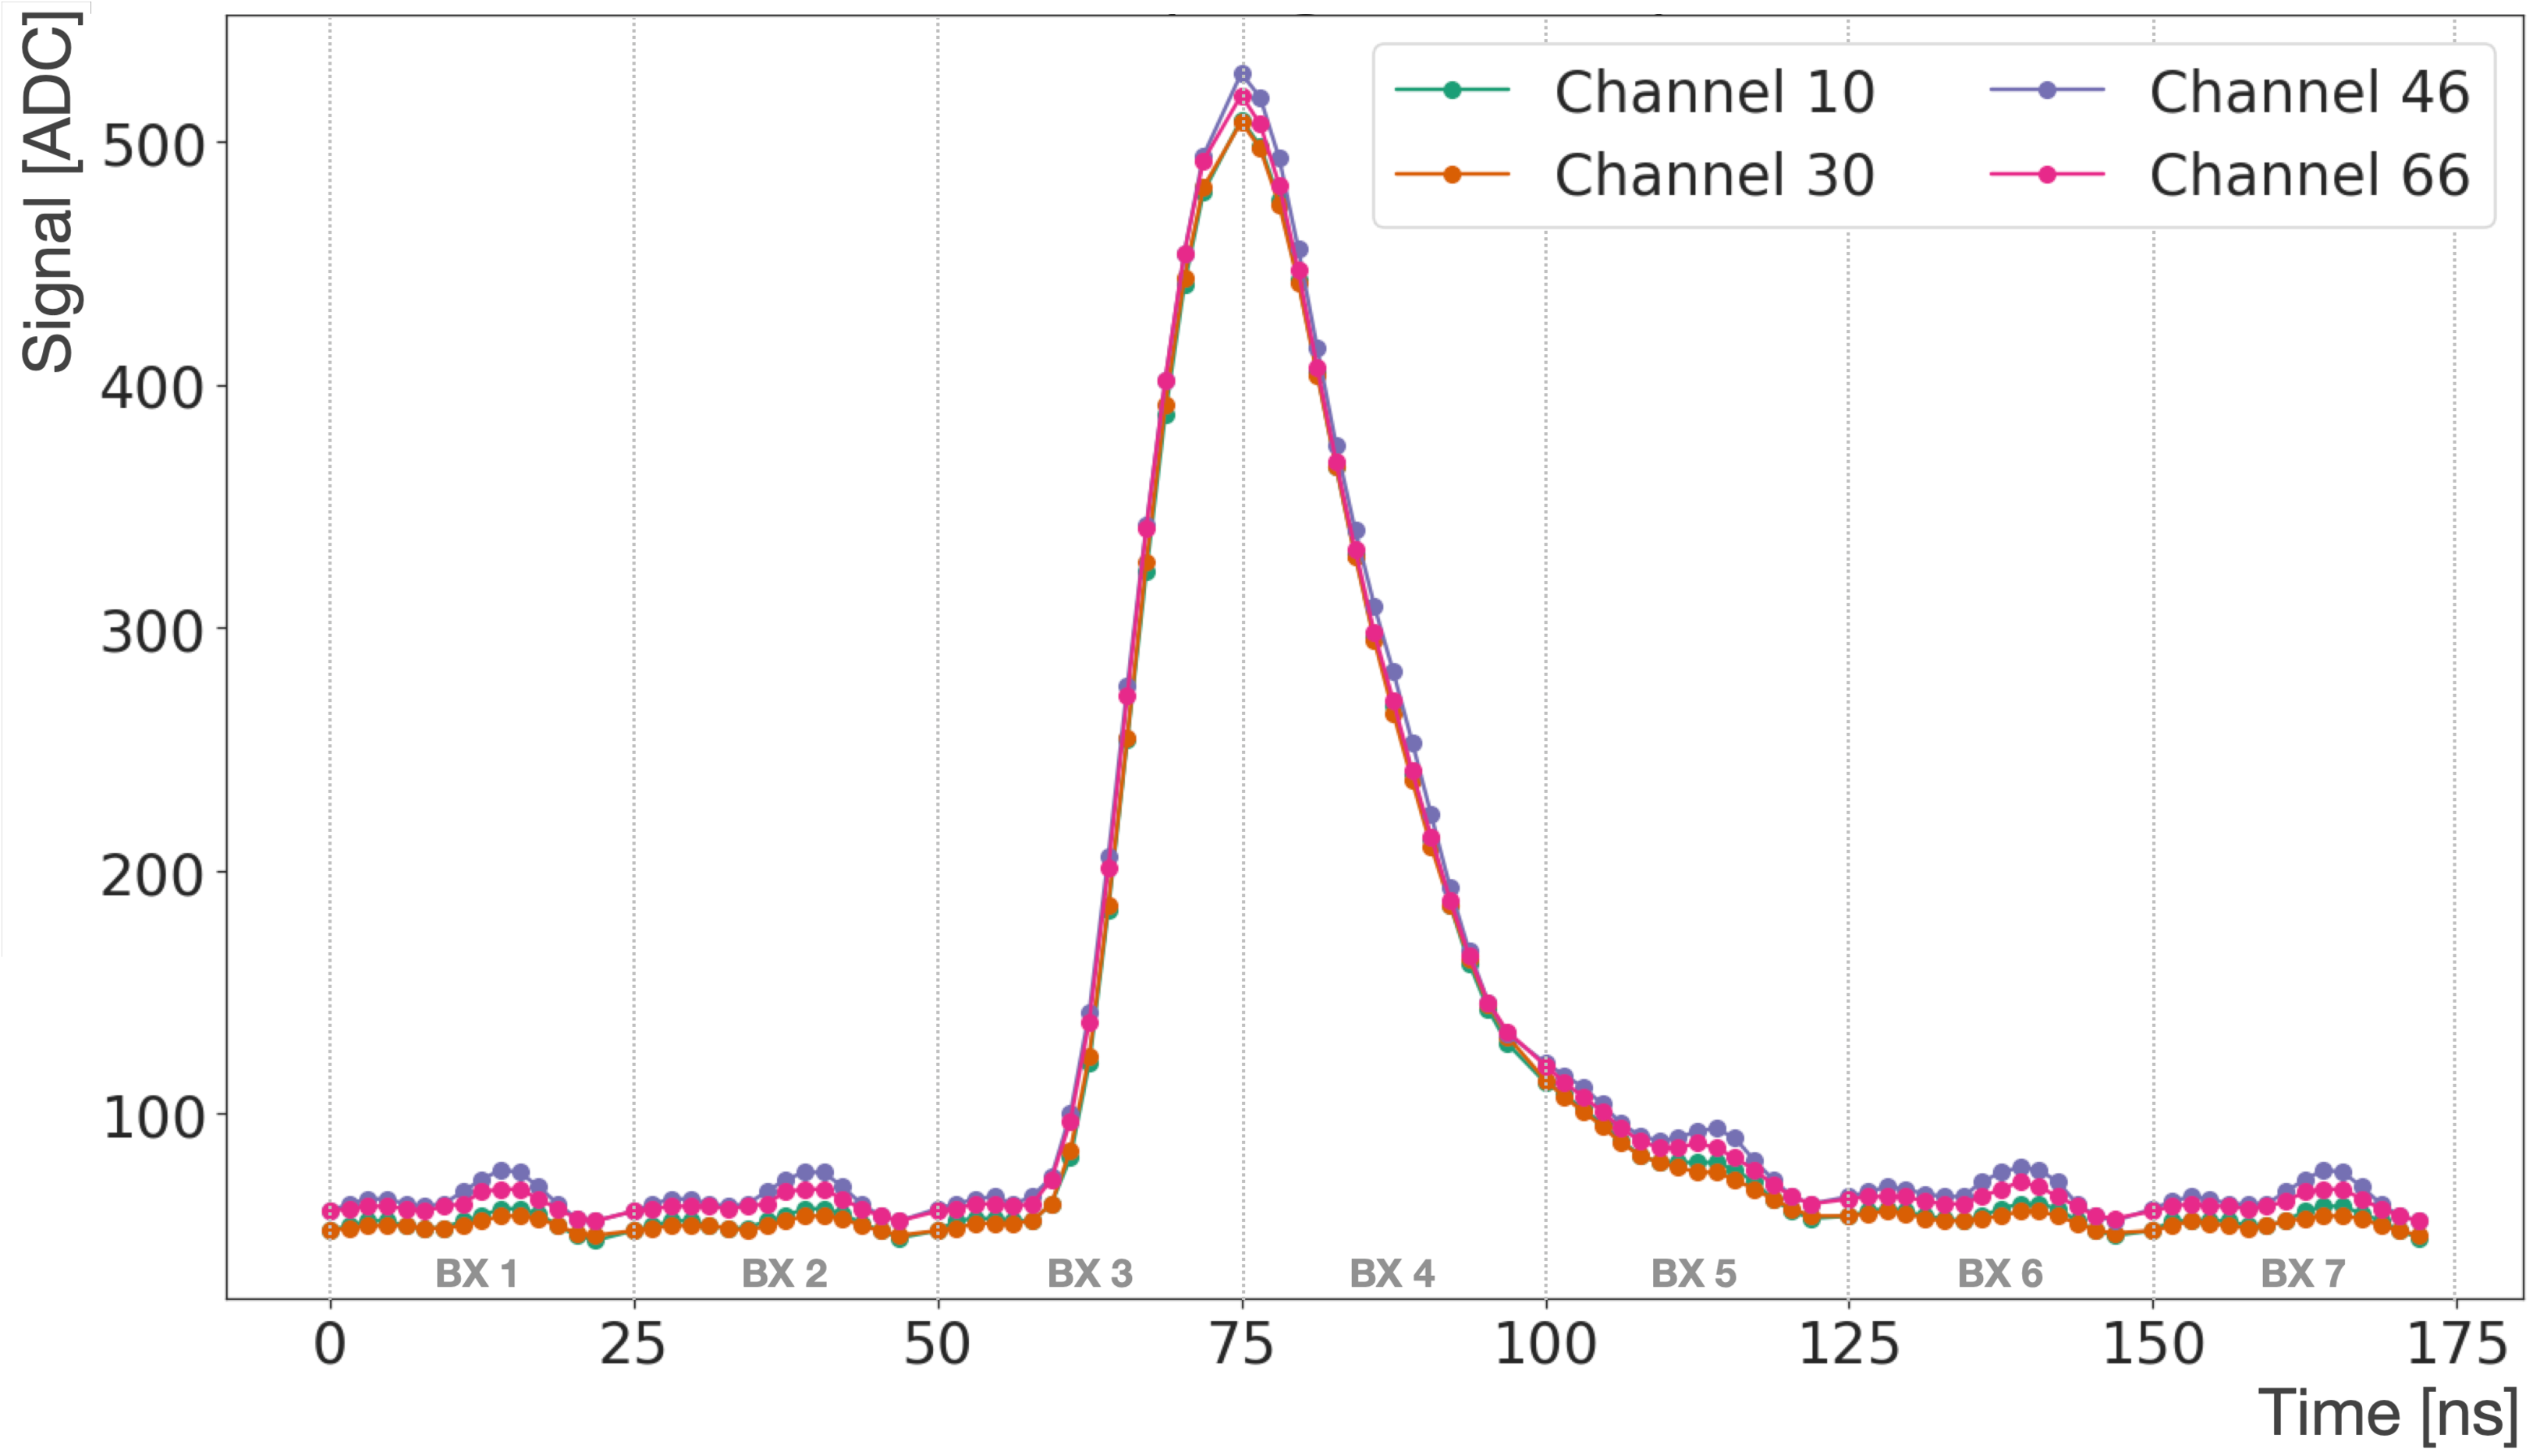
\includegraphics[width=0.65\linewidth]{Figures/HGCAL/BestPhase.pdf}
    \caption{Sampling scan of the ADC value of 4 channels for different phases. Each 25~ns bunch crossing (BX) period is divided into 16 phases: the sampling position is determined by the phase of the signal maximum.}
    \label{fig:BestPhase}
\end{figure}

\bigbreak

Other configurable parameters exist within the HGCROC3 I2C register but are not addressed in this context as they are not relevant to this context.

\subsection{The performance}
\label{subsec:The HGCROC3 performance}

Once the HGCROC3 is correctly configured for the data acquisition, it is possible to check that its performance aligns with the HGCAL FE electronics requirements.
The ASIC can measure charges spanning from 160~fC to 320~pC, with two different regimes: the ADC is calibrated to accurately detect charges up to the preamplifier saturation, and when the saturation is reached the Time-Over-Threshold (ToT) technique measures the signal duration over saturation. The transition from ADC to ToT is configurable through dedicated I2C parameters. The preamplifier output is also connected to the Time-Of-Arrival (ToA) discriminator to capture timing information. 
Considering the various types of signal pulses to be read out by the HGCROC3, it is essential to evaluate the response of the device to different signal amplitudes in terms of ADC, ToA and ToT.

\subsubsection{The ADC performance}
\label{subsubsec:The ADC performance}

The front-end ADC operates at 40 MHz to convert the analog signal into a digitised value corresponding to the signal amplitude and energy deposit in the detector. 
Figure~\ref{fig:FitSampling} shows a typical signal pulse recorder by the HGCROC3 and modelled by the following equation:

\begin{equation}
    f(t) = A_{0}\,e^{-at}\left[e^{-ct}\left(\frac{t^3}{c}-\frac{3t^2}{c^2}+\frac{6t}{c^3}-\frac{6}{c^4}\right)+\frac{6}{c^4}\right], \;\; a =\frac{1}{\tau_{p}}, \;\; c=\frac{1}{\tau_{p}}-\frac{1}{\tau_{s}}
\label{eq:FitSampling}
\end{equation}

where $\tau_{p}$ and $\tau_{s}$ correspond to the characteristic time of the preamplifier and of the shaper circuit respectively.
The model well describes the recorded data, with minor discrepancies below 2\%.

\begin{figure}
    \centering
    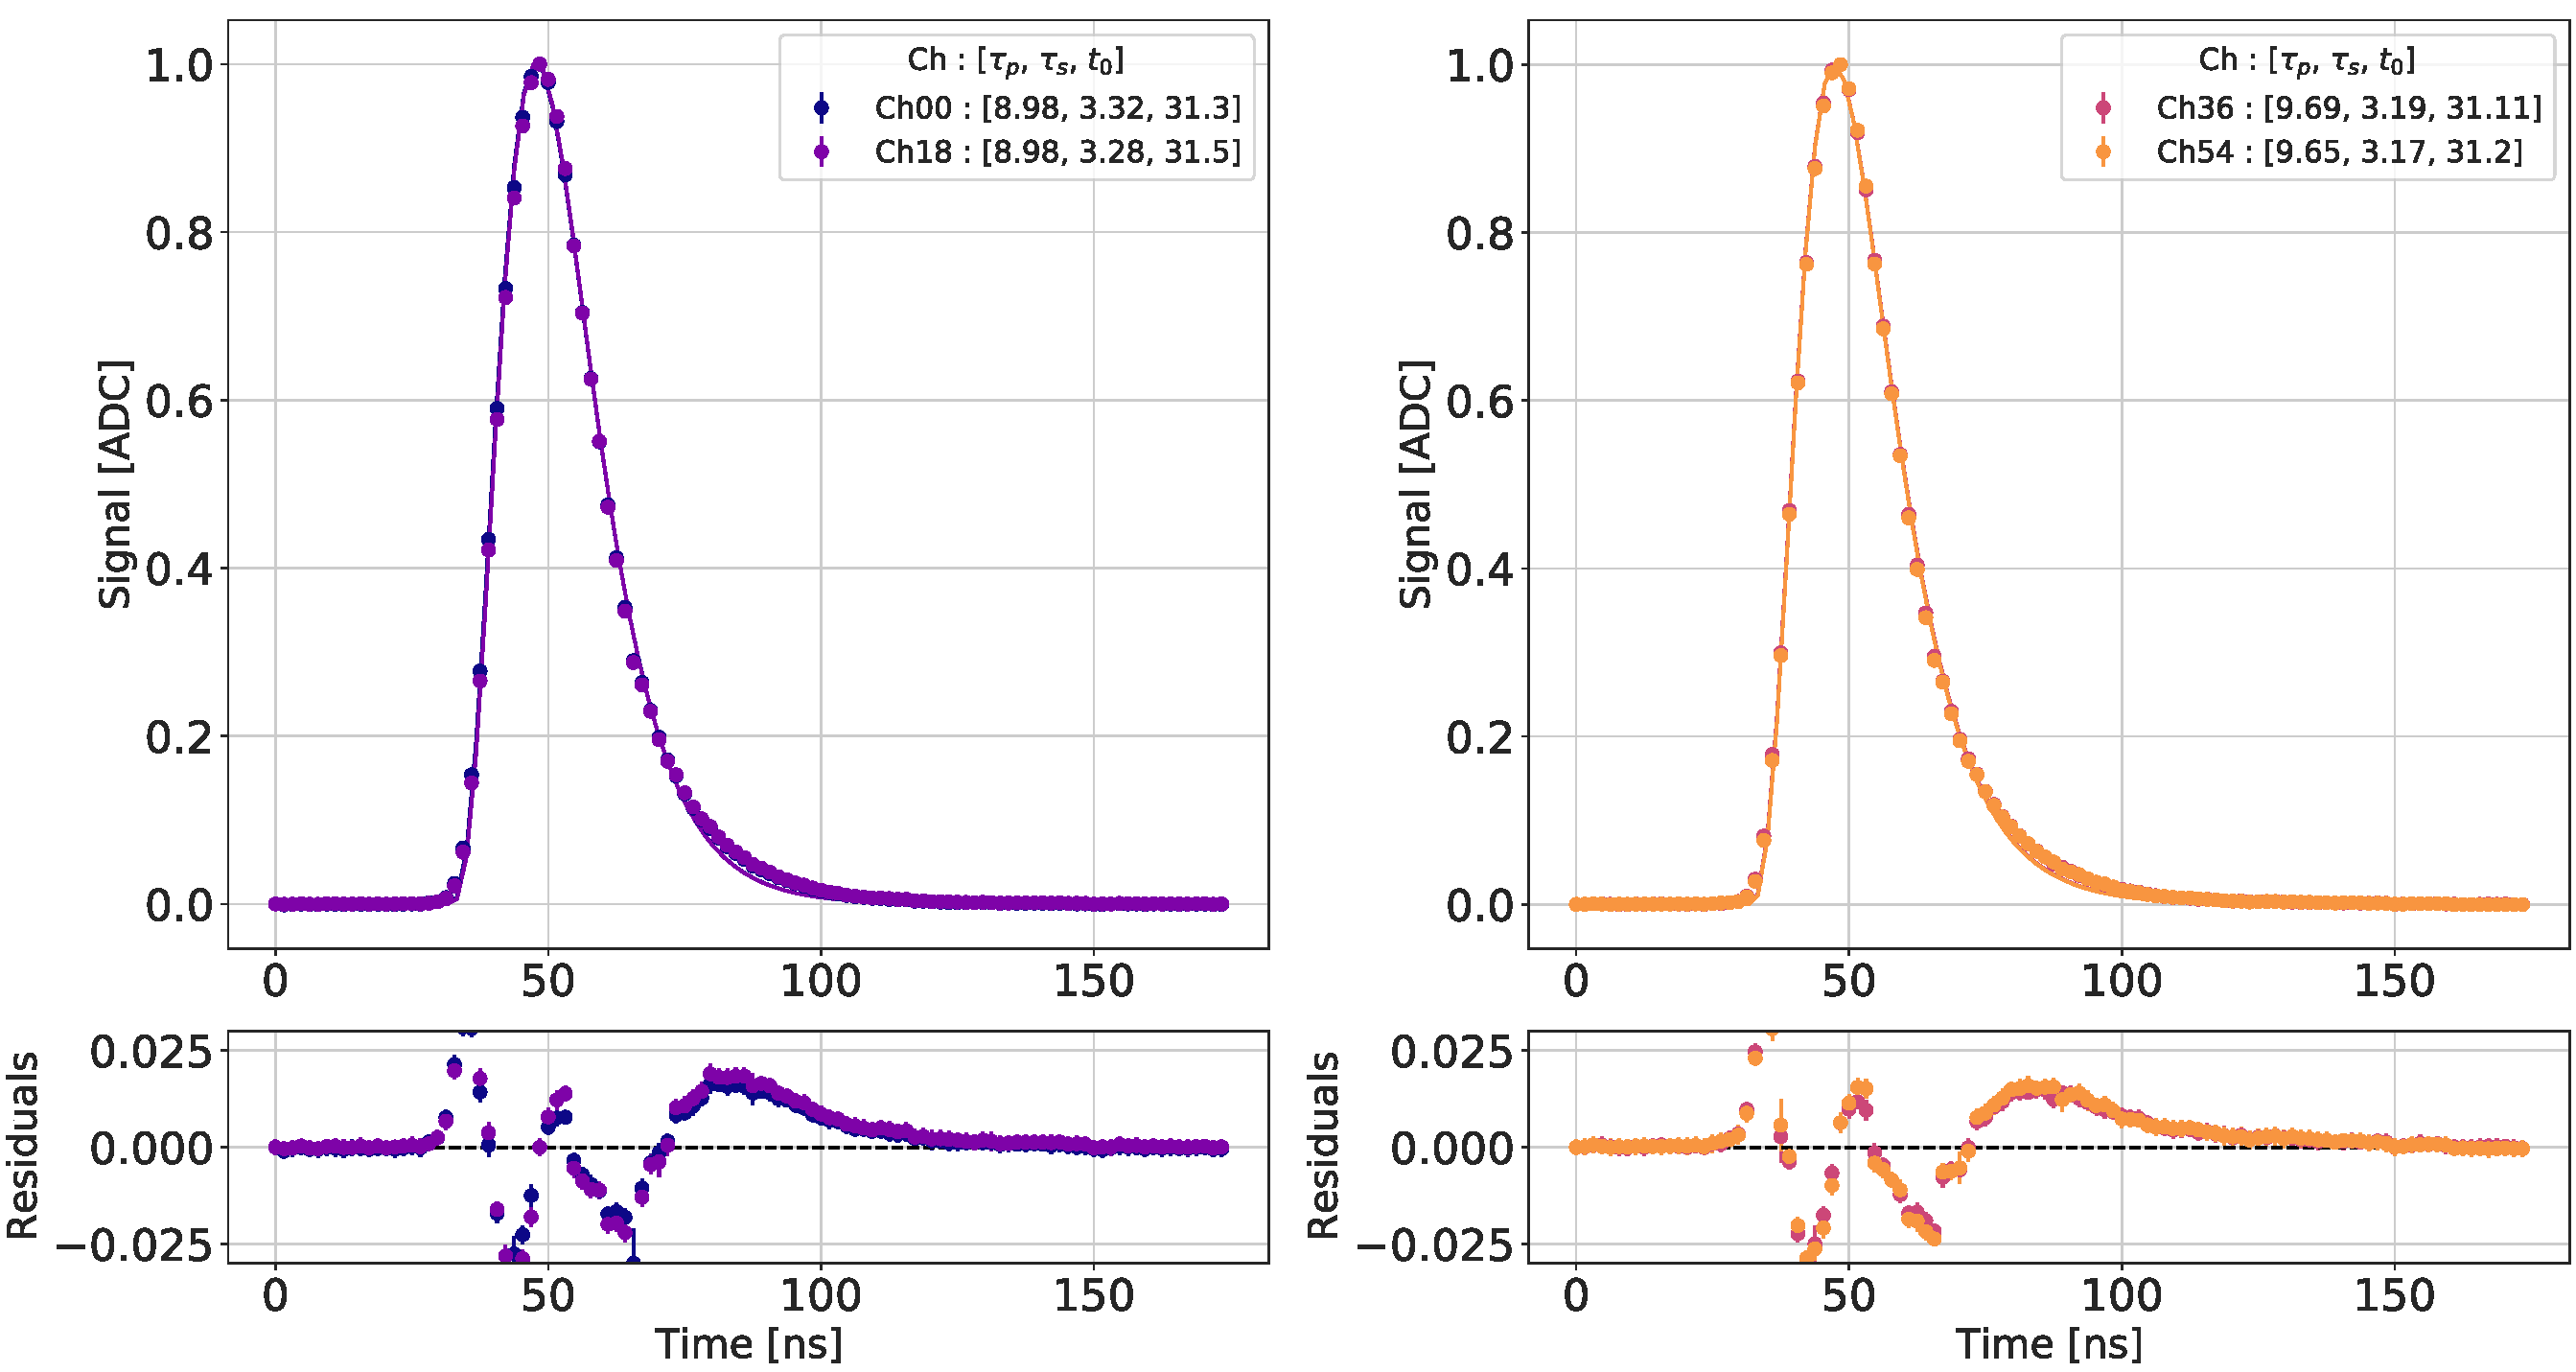
\includegraphics[width=0.75\linewidth]{Figures/HGCAL/FitSampling.pdf}
    \caption{Normalised signal pulse for 4 channels of the HGCROC3, two channels of the first half (left) and two channels of the second half (right). The signal shape is fitted using Equation~\ref{eq:FitSampling} and the optimised parameters of the fit are reported in the legend. Discrepancies between the model and the data are below 2\%.}
    \label{fig:FitSampling}
\end{figure}

\bigbreak

During HL-LHC operations, the dense data stream will not support the transmission of the full analog signal. Only one quantity will be transmitted to the back-end electronics and used for the offline event reconstruction: the signal amplitude. The role of the ADC circuit is to provide a clean signal shape, with an amplitude directly proportional to the injected charge in the whole dynamic range.
The ADC linearity is tested by injecting signals with increasing charge values and measuring the response of the recorded ADC as a function of the input charge. Figure~\ref{fig:ADC_Injection} shows the expected linear response of the signal amplitude measured by the HGCROC3 with respect to the injected charge, in units of the \texttt{Calib\_DAC} parameter - 100~\texttt{Calib\_DAC} corresponds to a charge of 120~fC. A linear function is used to test the linearity of the response:
\begin{equation}
    f(t) = ax + b
\label{eq:ADCLinearity}
\end{equation}

The best parameters, extracted from the fit, are reported in the legend for each channel.

\begin{figure}
    \centering
    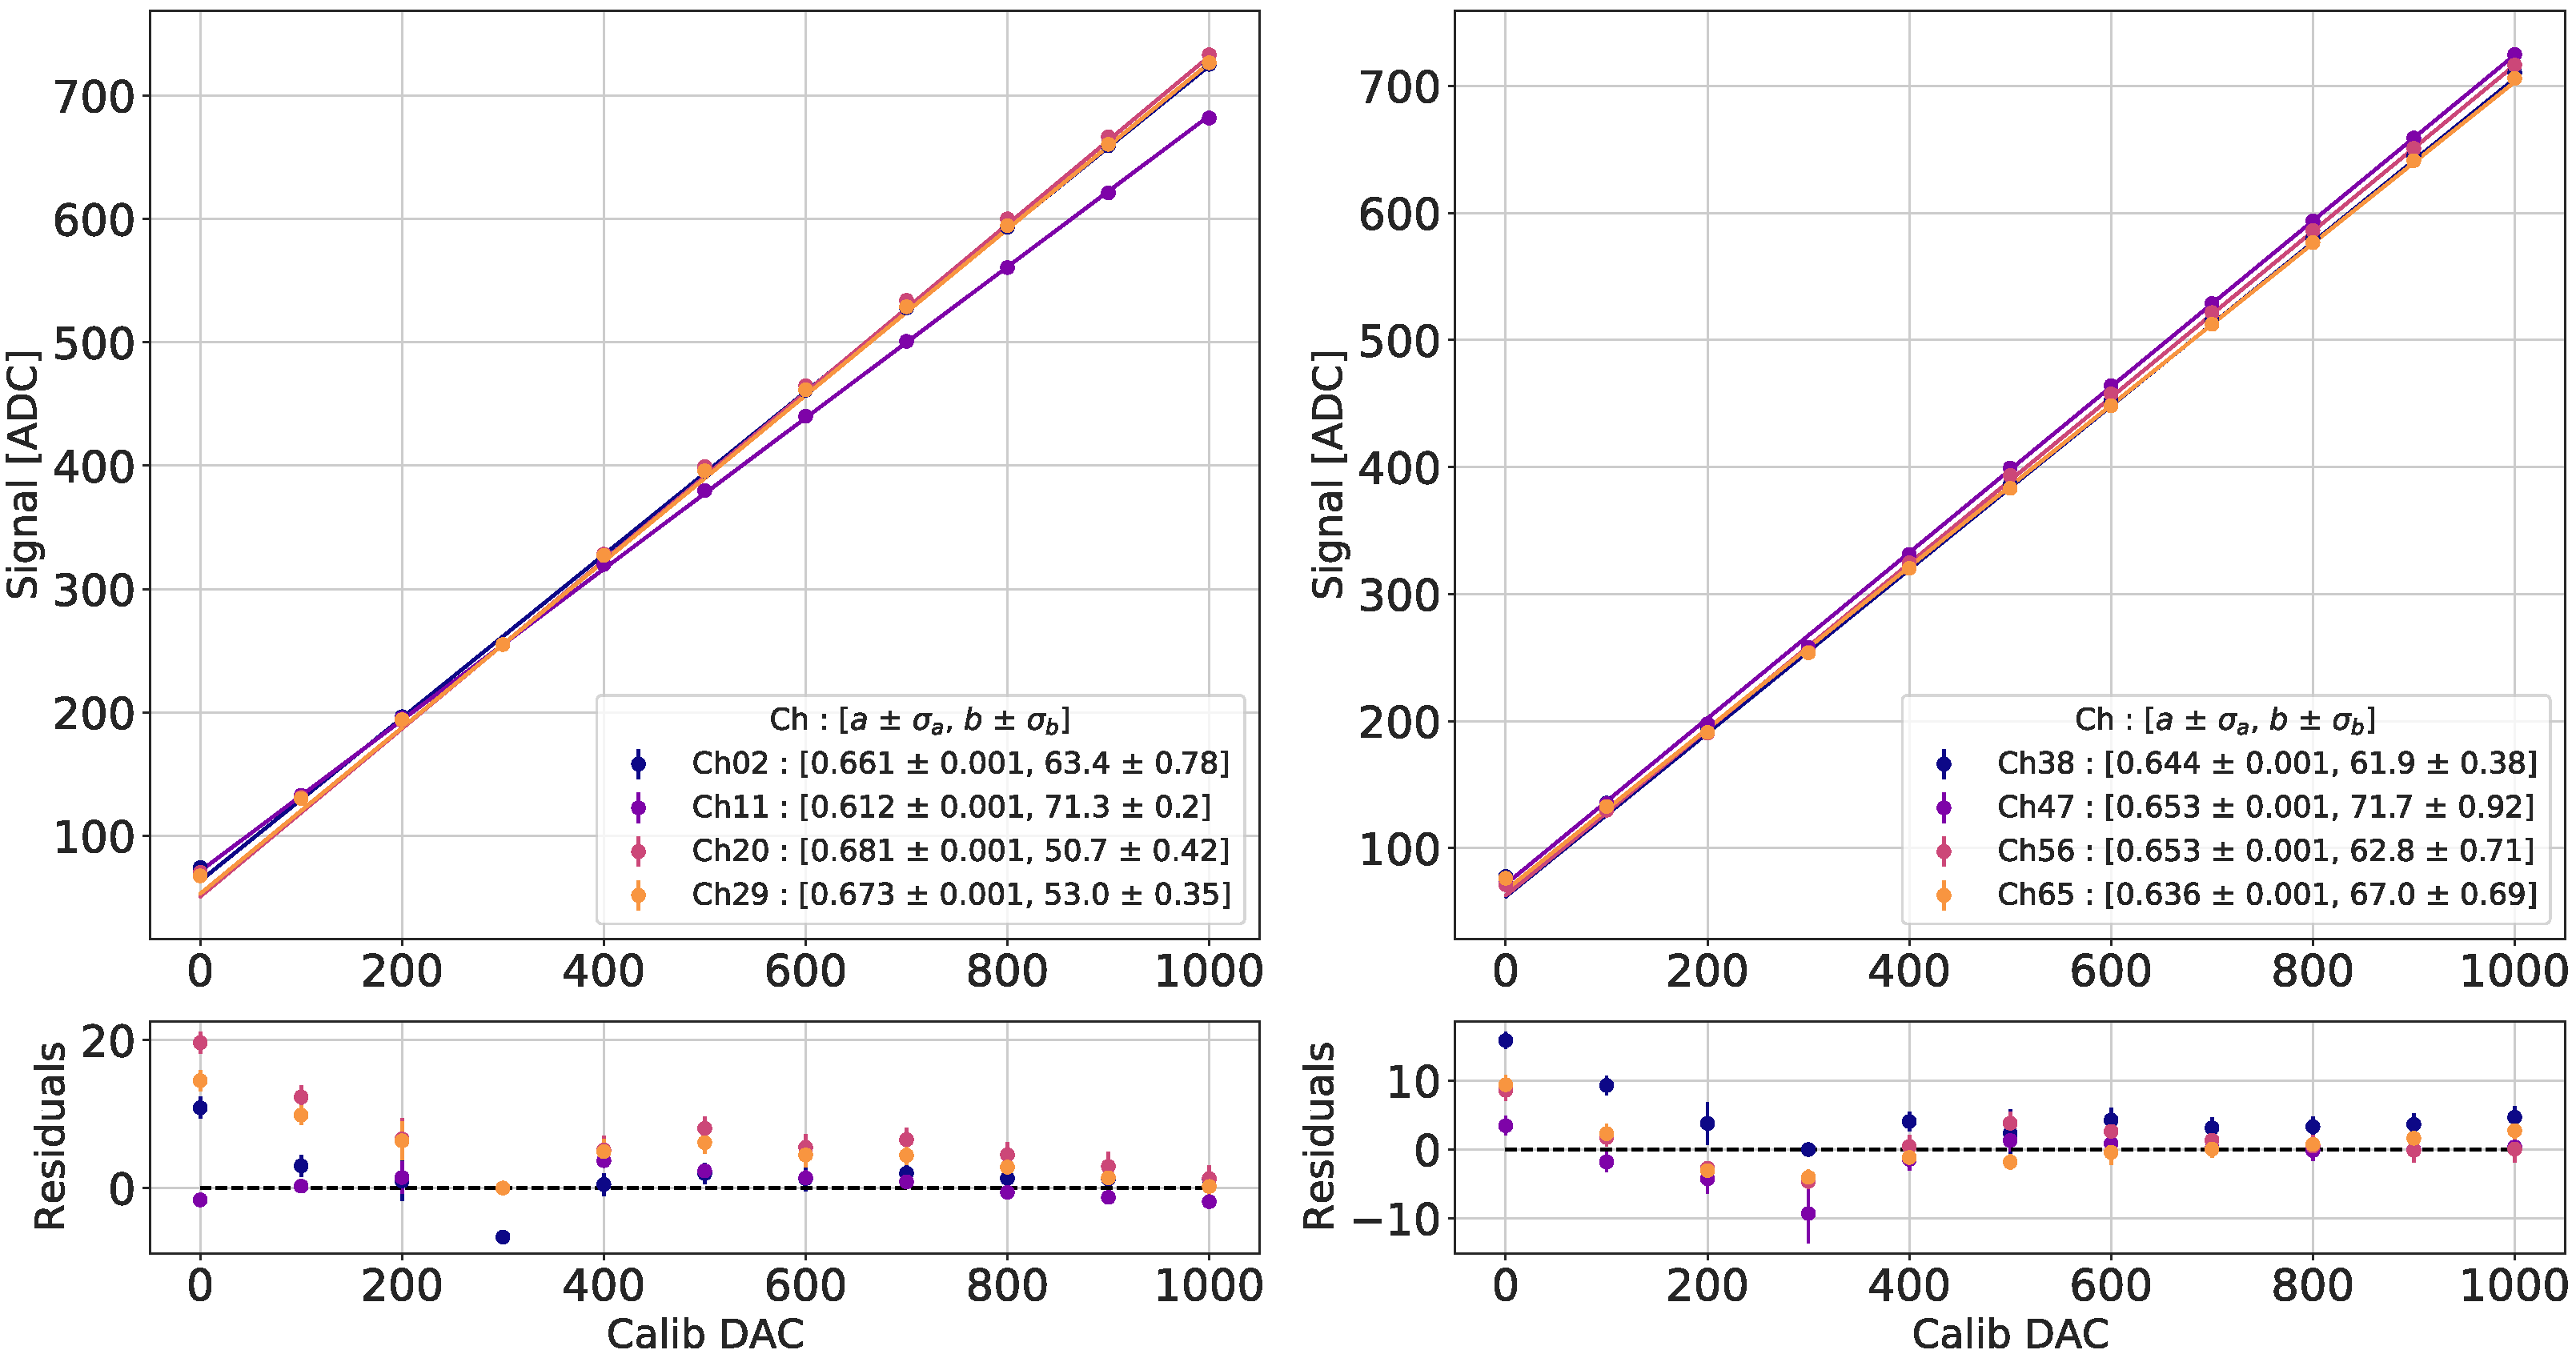
\includegraphics[width=0.7\linewidth]{Figures/HGCAL/ADC_Injection.pdf}
    \caption{The ADC response linearity to multiple injections corresponding to different \texttt{Calib\_DAC} values, defining the input charge. The  response is fitted with the linear function in Equation~\ref{eq:ADCLinearity} and the optimised parameters of the fit are reported in the legend.}
    \label{fig:ADC_Injection}
\end{figure}

\subsubsection{The ToT performance}
\label{subsubsec:The ToT performance}

\begin{figure}[b!]
    \centering
    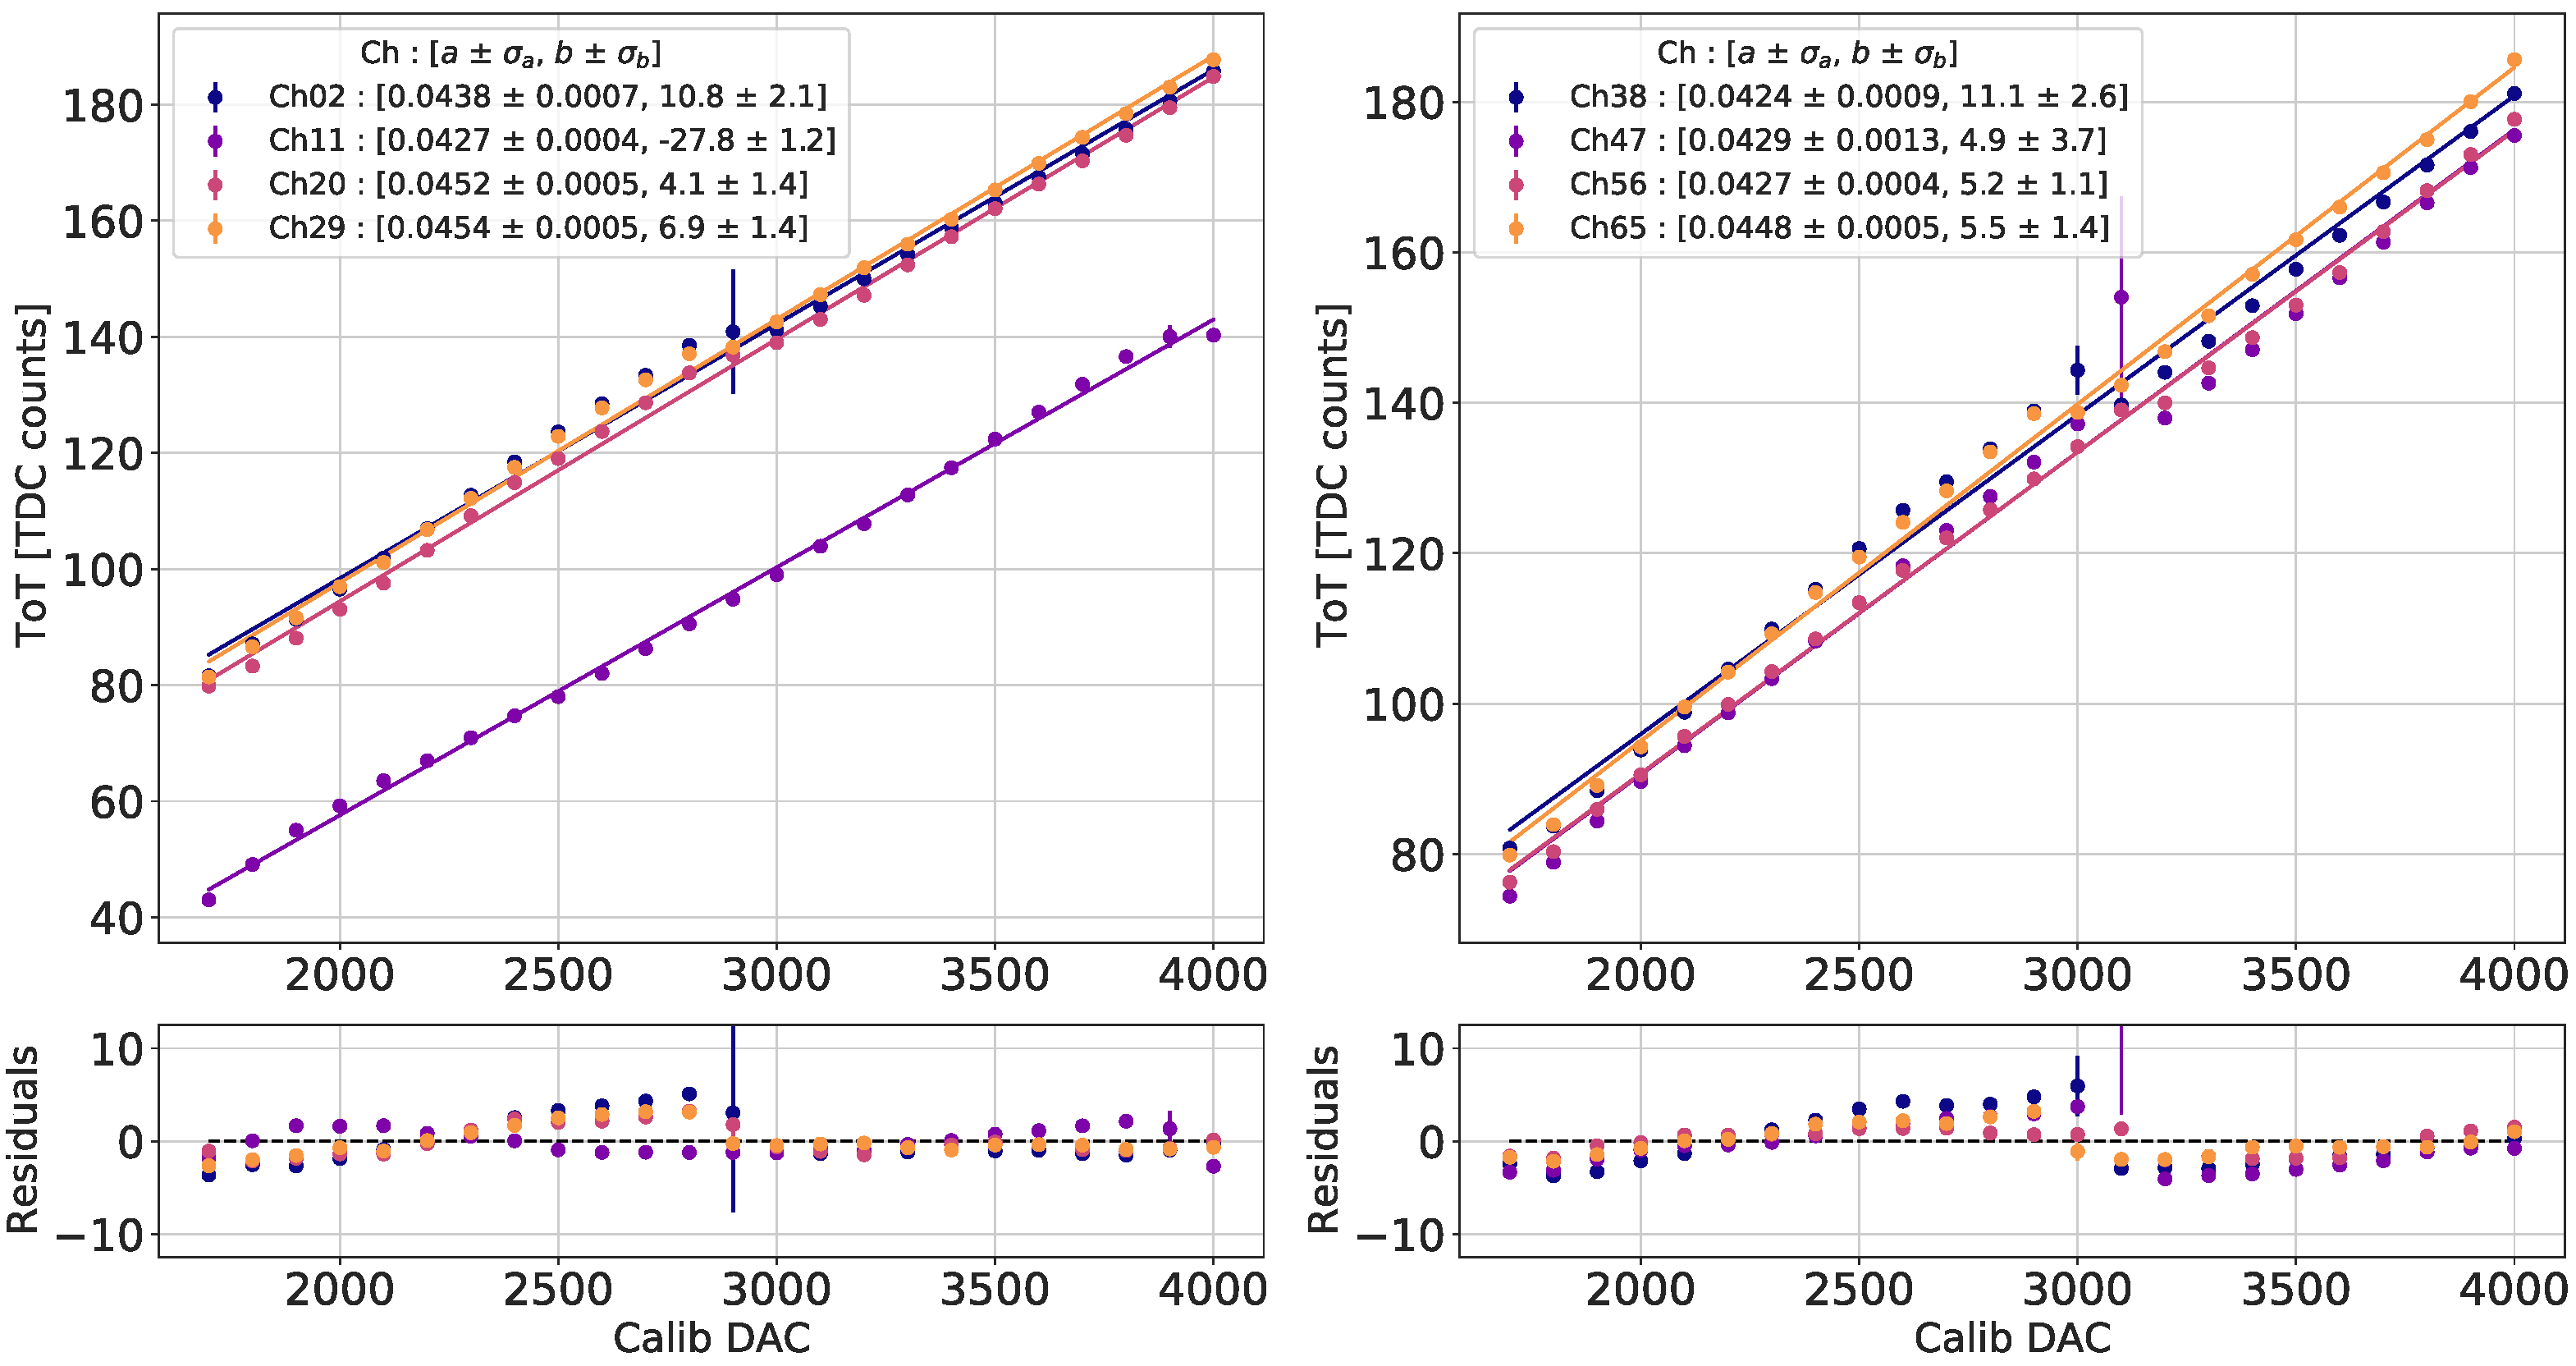
\includegraphics[width=0.7\linewidth]{Figures/HGCAL/TOT_Injection.pdf}
    \caption{The ToT response linearity to multiple injections corresponding to different \texttt{Calib\_DAC} values, defining the input charge. The  response is fitted with the linear function in Equation~\ref{eq:ADCLinearity} and the optimised parameters of the fit are reported in the legend.}
    \label{fig:TOT_Injection}
\end{figure}

When the preamplifier enters the saturation regime, the signal duration becomes proportional to the injected charge. Consequently, it is possible to estimate the signal amplitude through an indirect measurement of its saturation duration.

The Time-over-Threshold (ToT) technique measures the time difference between the start and the end of the saturation time. Figure~\ref{fig:TOT_Injection} illustrates the ToT measurements for different injected charges. The ToT curve is fitted by using Equation~\ref{eq:ADCLinearity} and the performance show a good linearity up to the highest charge of 500~fC. 

\subsubsection{The ToA performance}
\label{subsubsec:The ToA performance}

The time measurements are crucial to discriminate pile-up events and improve the particle identification in collision scenarios. This information is encoded in the Time-of-Arrival (ToA), corresponding to the time at which the signal amplitude exceeds the ToA threshold value.

The ToA measurement noticeably depends on the signal amplitude, since higher signals reach the discriminator threshold faster, while lower signals require more time to reach the threshold. This common behaviour is usually known as \textit{"time walk"} and needs to be considered as a correction when providing the time information.
Figure~\ref{fig:TOA_Injection} shows the time walk curve of the ToA measurement as a function of the signal amplitude. The time walk is parametrically described by Equation~\ref{eq:TOATimeWalk} and the results for the fit parameters are reported for each channel in the legend.

\begin{equation}
    f(t) = \frac{a}{x-x_0}+b
\label{eq:TOATimeWalk}
\end{equation}

\bigbreak

\begin{figure}
    \centering
    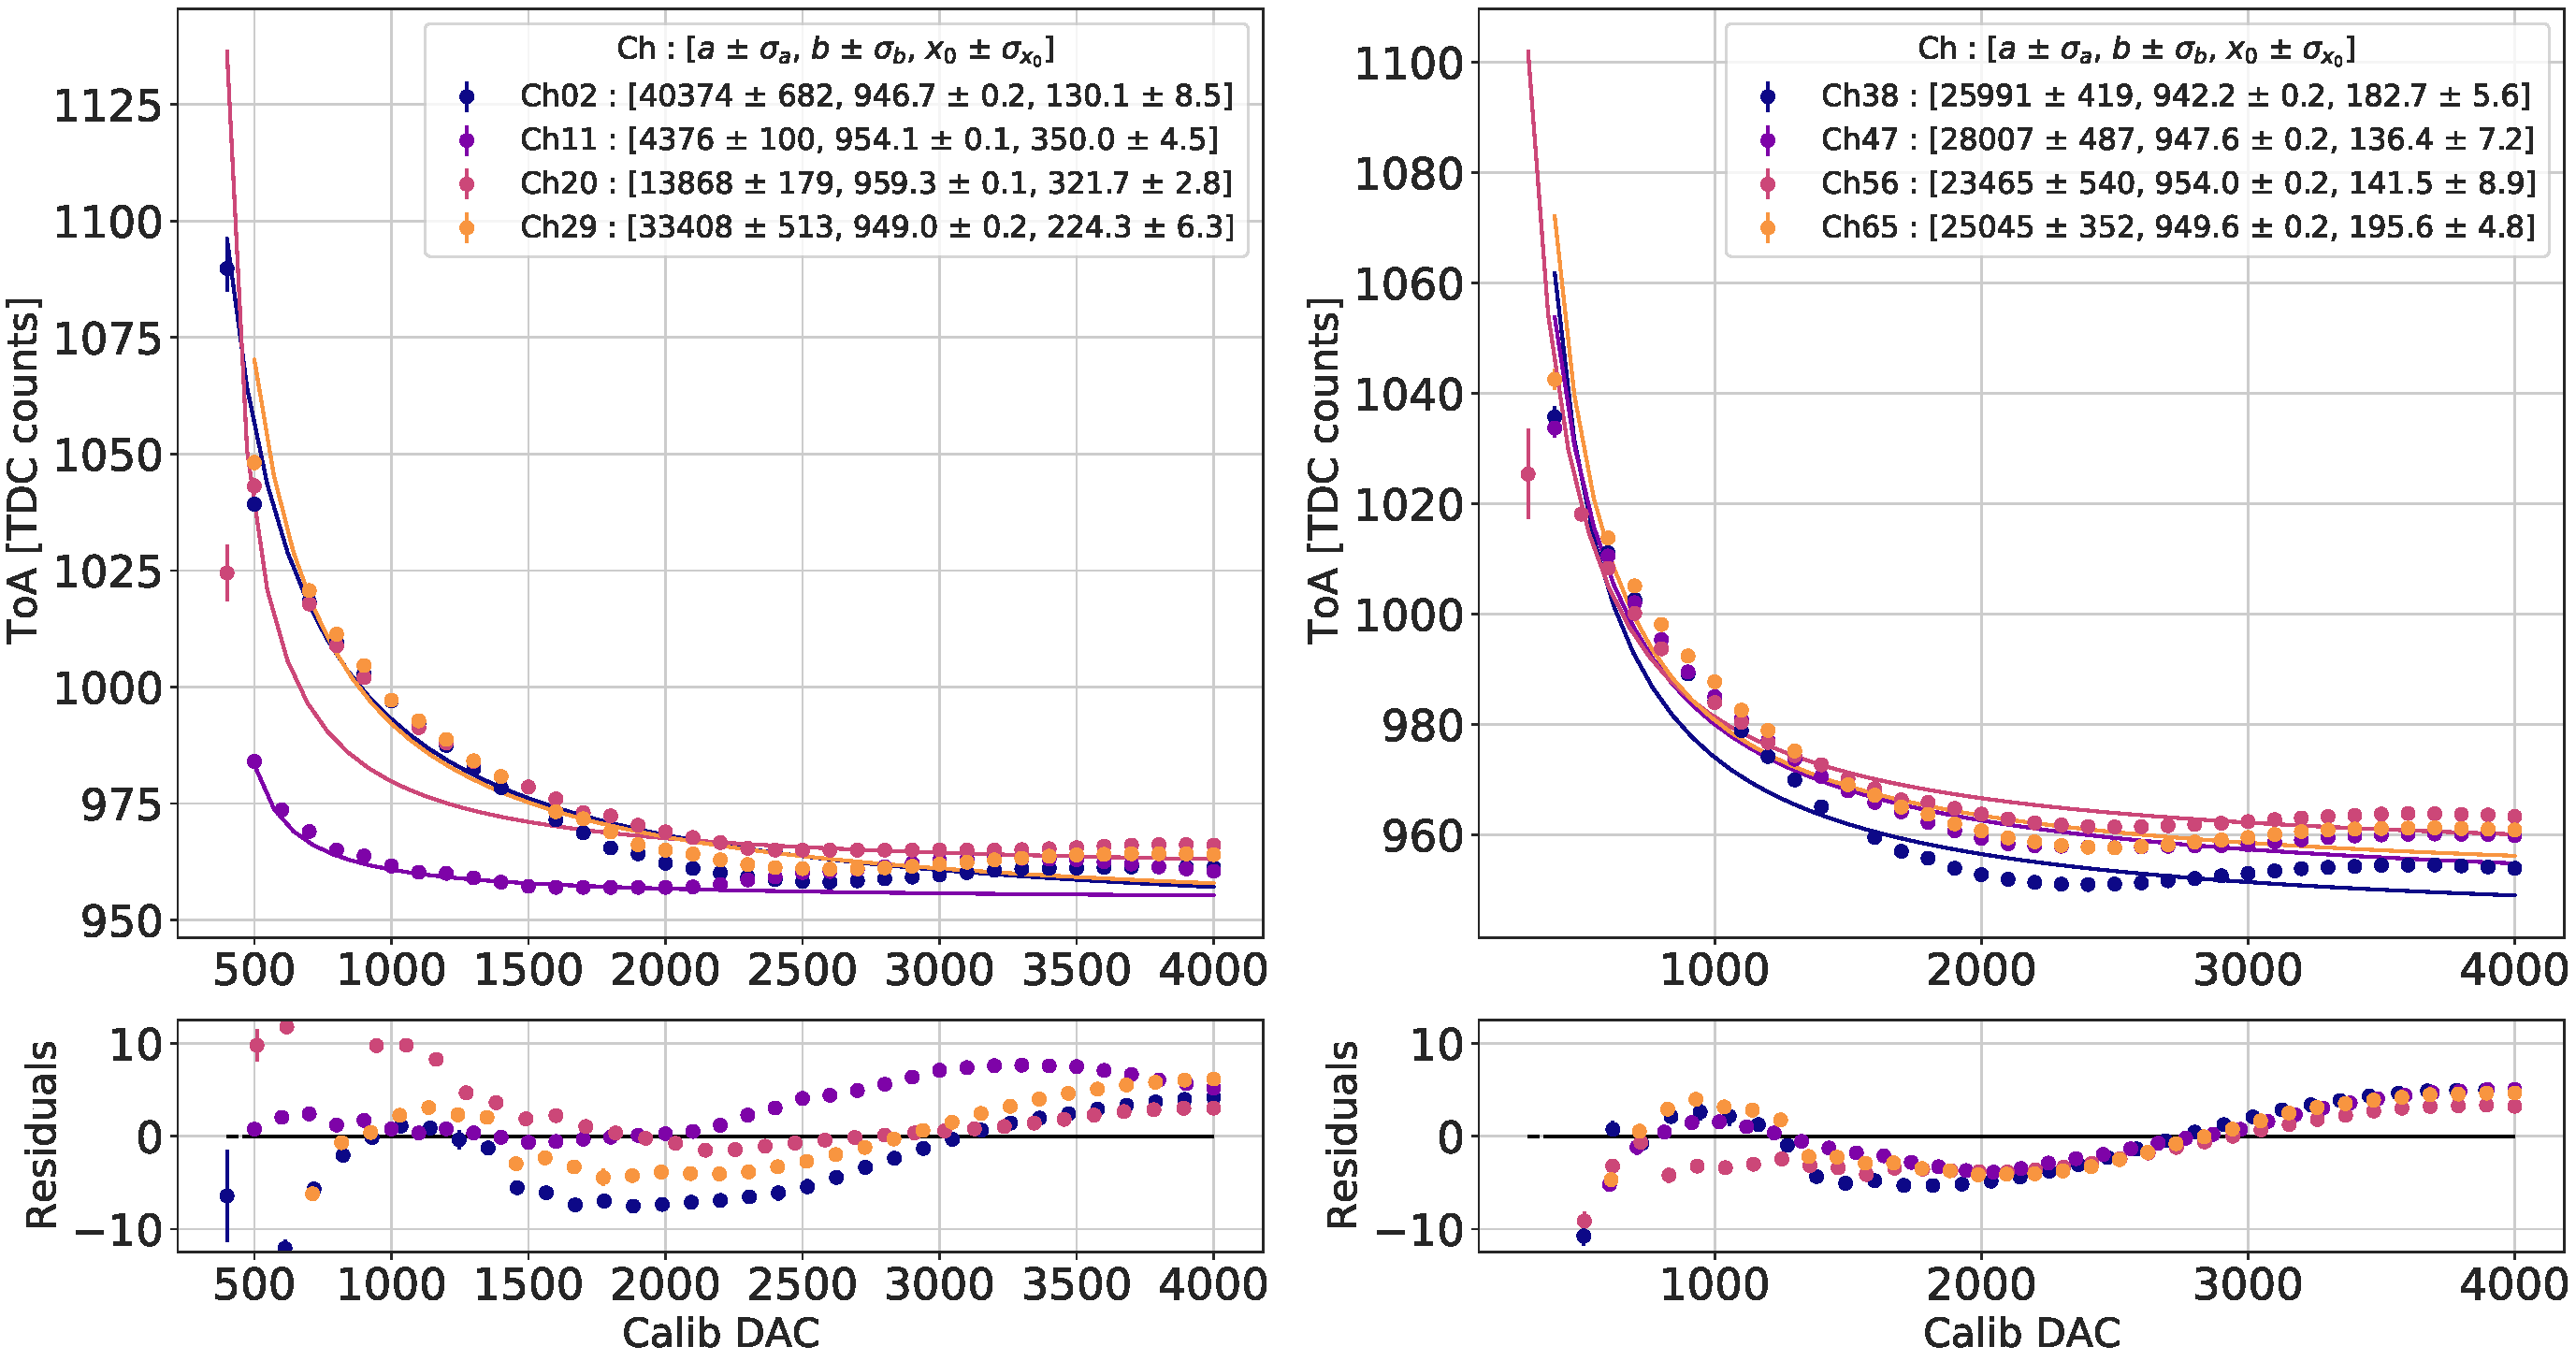
\includegraphics[width=0.7\linewidth]{Figures/HGCAL/TOA_Injection.pdf}
    \caption{The \textit{"time walk"} curve describing the ToA response to multiple injections corresponding to different \texttt{Calib\_DAC} values, defining the input charge. The  response is fitted with the function in Equation~\ref{eq:TOATimeWalk} and the optimised parameters of the fit are reported in the legend.}
    \label{fig:TOA_Injection}
\end{figure}

\begin{figure}[b!]
    \centering
    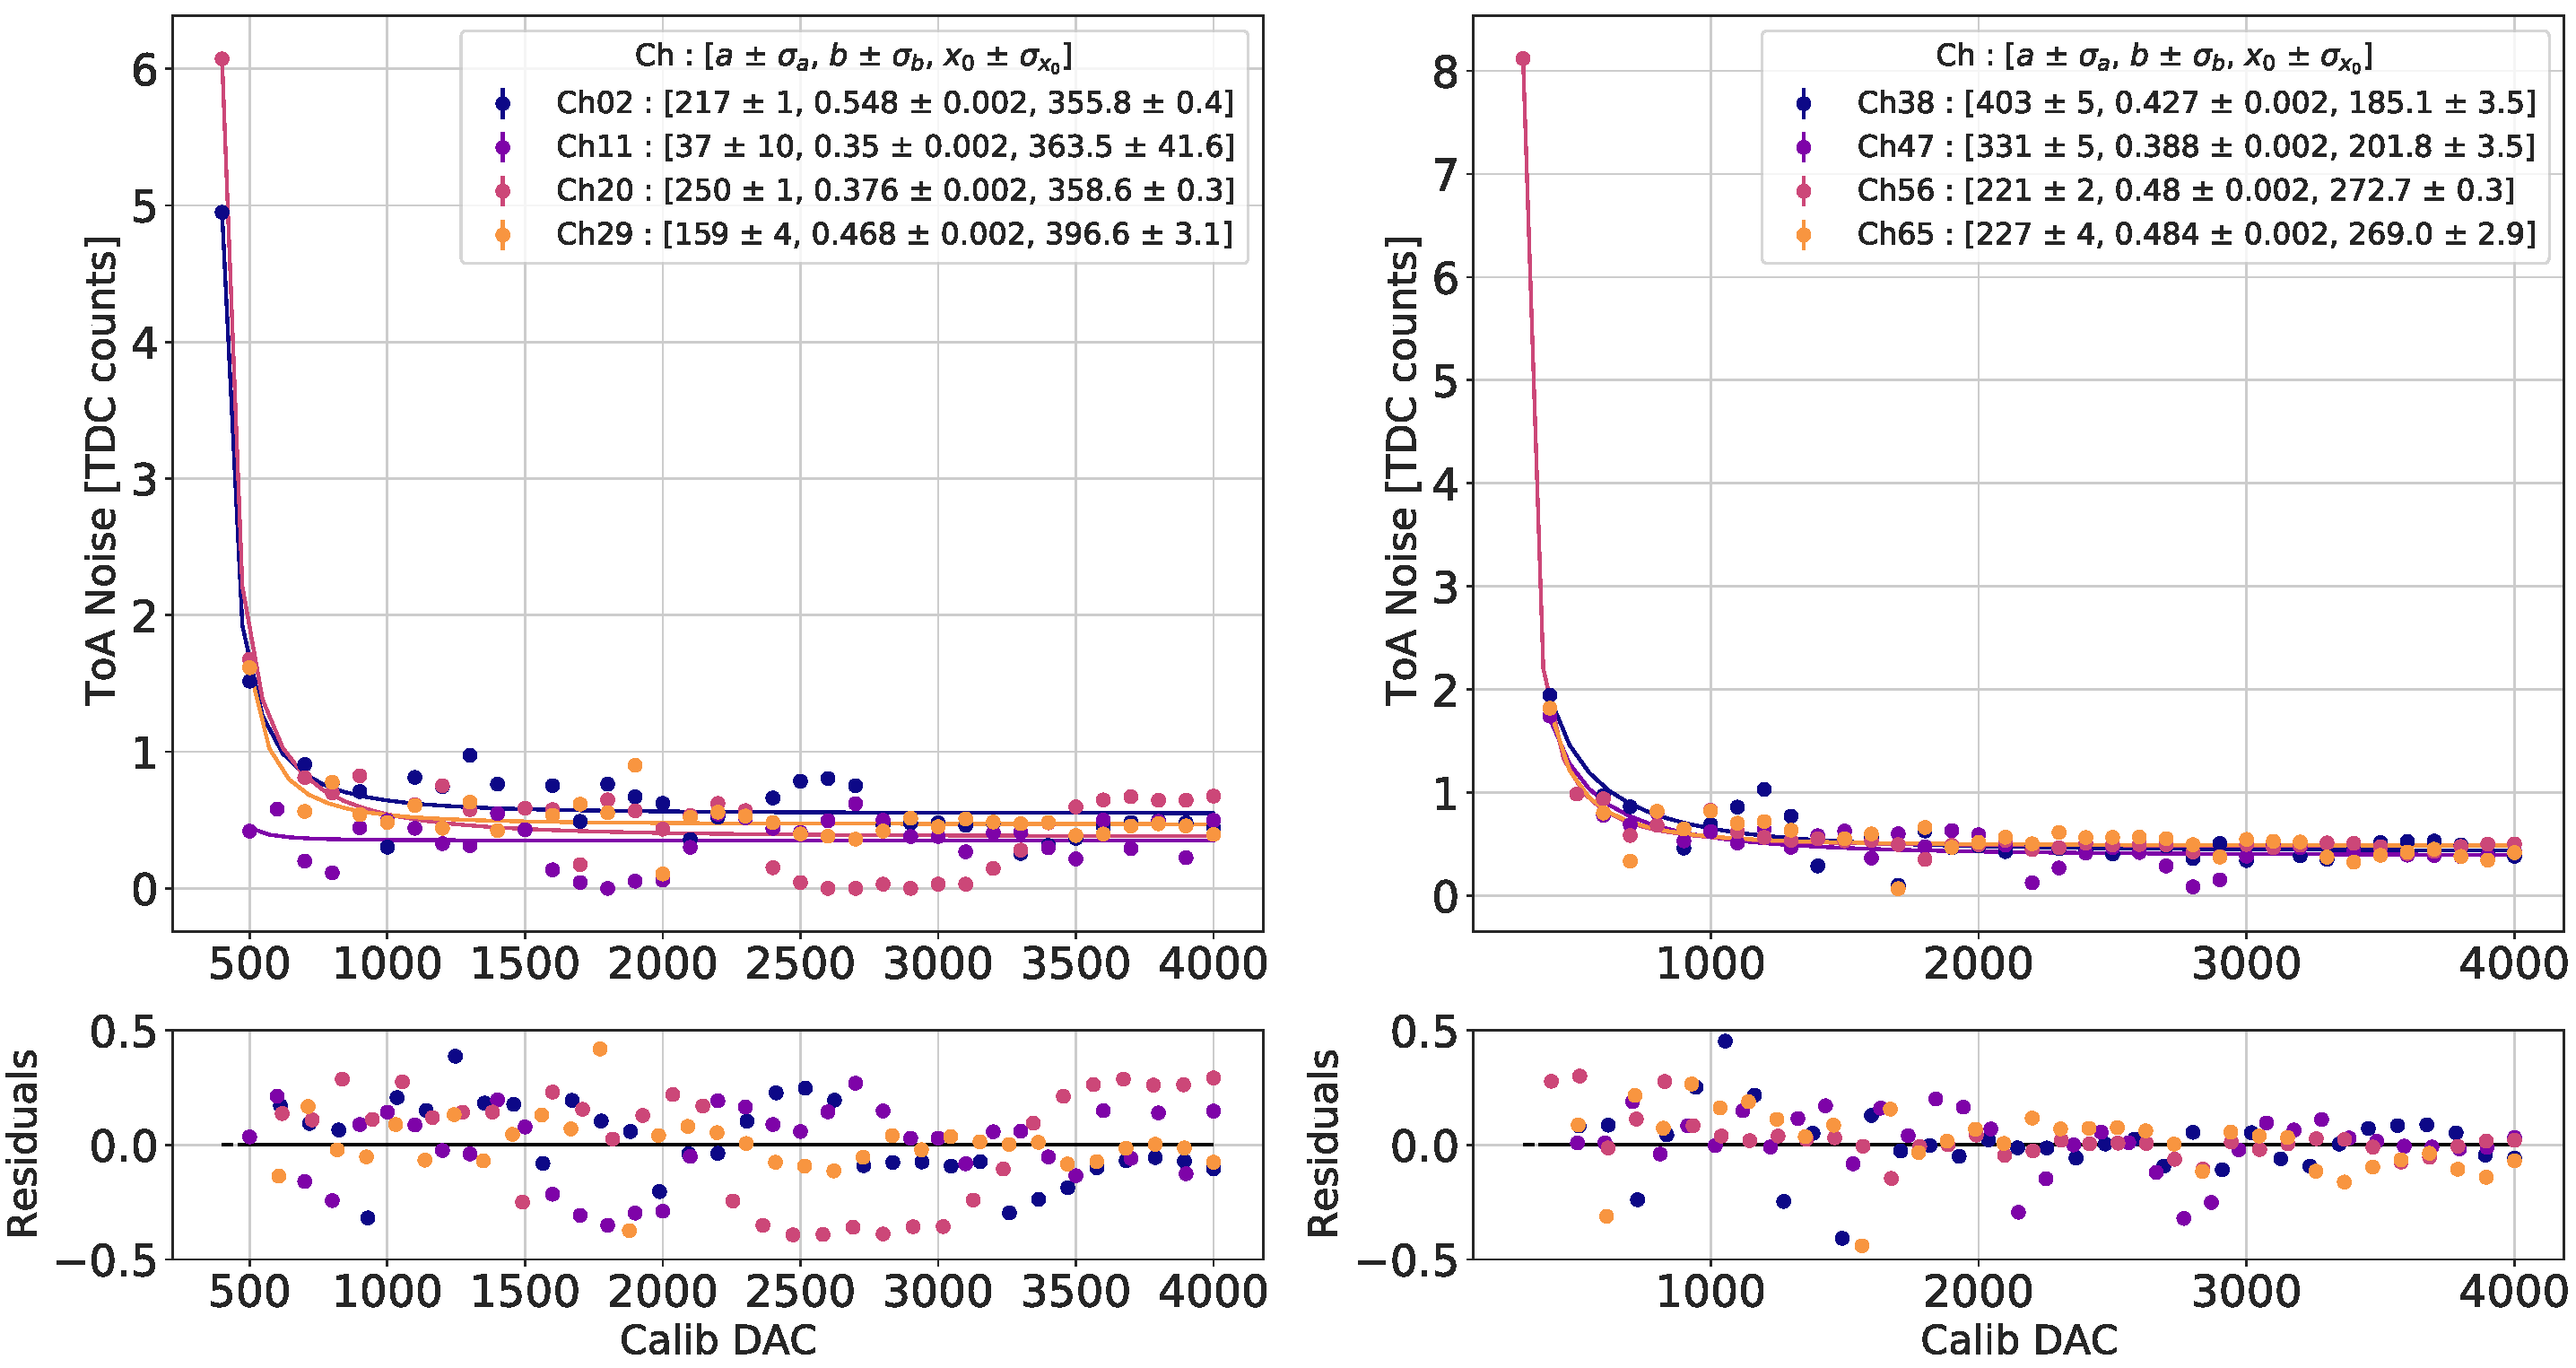
\includegraphics[width=0.7\linewidth]{Figures/HGCAL/ToANoise_Injection.pdf}
    \caption{The \textit{"time jitter"} curve describing the ToA noise to multiple injections corresponding to different \texttt{Calib\_DAC} values, defining the input charge. The  response is fitted with the function in Equation~\ref{eq:TOATimeJitter} and the optimised parameters of the fit are reported in the legend.}
    \label{fig:TOANoise_Injection}
\end{figure}

For the HGCROC3 performance it is also interesting to evaluate the effect of the electronic noise on the time measurements. Amplitude variations due to electronic noise introduce an uncertainty on the timing of a signal crossing the defined threshold: the effect will be more accentuated for a low amplitude signal than for a high amplitude signal.

The \textit{"time jitter"} curve, describing the uncertainty on the timing measurement due to the electronic noise, is shown in Figure~\ref{fig:TOANoise_Injection}.
The trend can be described by Equation~\ref{eq:TOATimeJitter} and the parameters of the fit are reported in the legend of the plots.

\begin{equation}
    f(t) = \sqrt{\left(\frac{a}{x-x_0}\right)^2+b^2}
\label{eq:TOATimeJitter}
\end{equation}

\subsection{The batch testing}
\label{subsec:The HGCROC3 batch testing}

The HGCAL detector is expected to host approximately 120,000 HGCROC3 read-out chips. The large number of ASICs poses significant challenges in both manufacturing and production, making it difficult to ensure each prototype meets its design specifications.
To guarantee high-quality standards for each HGCROC3 device, all the newly produced HGCROC3 chips will undergo production testing, with the target of determining whether a given ASIC should be assembled on a hexaboard or should instead be rejected due to production defects or bad performance.
The production testing will be conducted at the Laboratorie Leprince-Ringuet and the Omega facility. 
It will take place as an automated process, carried out by a robotic arm able to move the chips to the testing location, where a series of tests will be performed. 
These tests will examine the main components and parameters of the chips to ensure they are correctly configurable, can communicate with the software interface, and meet expected performance.

\bigbreak

In order to gain statistics about the HGCROC3 performance and optimise the testing procedure, a preliminary batch testing has been conducted on 200 prototypes of HGCROC3. Since the robotic arm was still under development, the batch testing has been performed using the manual socket board, where the chip can be inserted manually by means of a dedicated suction pen, as shown in Figure~\ref{fig:ManualSocket}.
The testing procedure is composed of an initial calibration, as described in Section~\ref{subsec:The calibration procedure}, and of a series of charge injections to assess the response of the device to different signal amplitudes in terms of ADC, ToA and ToT, as described in Section~\ref{subsec:The HGCROC3 performance}.
The batch testing furnishes a good opportunity to tailor the testing procedure and the criteria to accept or reject the chips. At the same time, it allows one to collect enough statistics to spot recurring unexpected behaviours that might be linked to potential design issues.

The vast majority of the rejected chips, as expected, is due to the presence of non-connected channels, showing zero response due to manufacturing problems. 
However, other recurring unexpected behaviours in the chip performance have been observed, revealing design weaknesses. These issues have been thoroughly investigated to understand their causes and to find possible solutions to mitigate them. 

\begin{figure}[b!]
    \centering
    \includegraphics[width=0.75\linewidth]{Figures/HGCAL/ManualSocket.pdf}
    \caption{Experimental set-up for the preliminary batch testing of the HGCROC3. The manual socket board supports the testing of several prototypes in series: the socket can be manually opened or closed to extract or insert the chip.}
    \label{fig:ManualSocket}
\end{figure}

\subsubsection{Issue in TDC initialisation}
\label{subsubsec:Issue in TDC initialisation}

The first issue found is related to incorrect initialization of the TDC component. This problem manifests as an entire half of the chip being unable to provide ToA and ToT information; however, the ADC component is not affected and shows good performance. The particularity of this issue lies in its random occurrence: the same device tested multiple times will randomly either exhibit or not the problem. This behavior has been attributed to an incorrect initialization procedure of the TDC controller and can be fixed by simply changing the testing start-up sequence.
% Arounf 20 chips were showing the problem, but since it's not a chip-related problem, all of them could recover after testing the device multiple times.

\subsubsection{Issue in ADC conversion}
\label{subsubsec:Issue in ADC conversion}

\begin{figure}
    \centering
    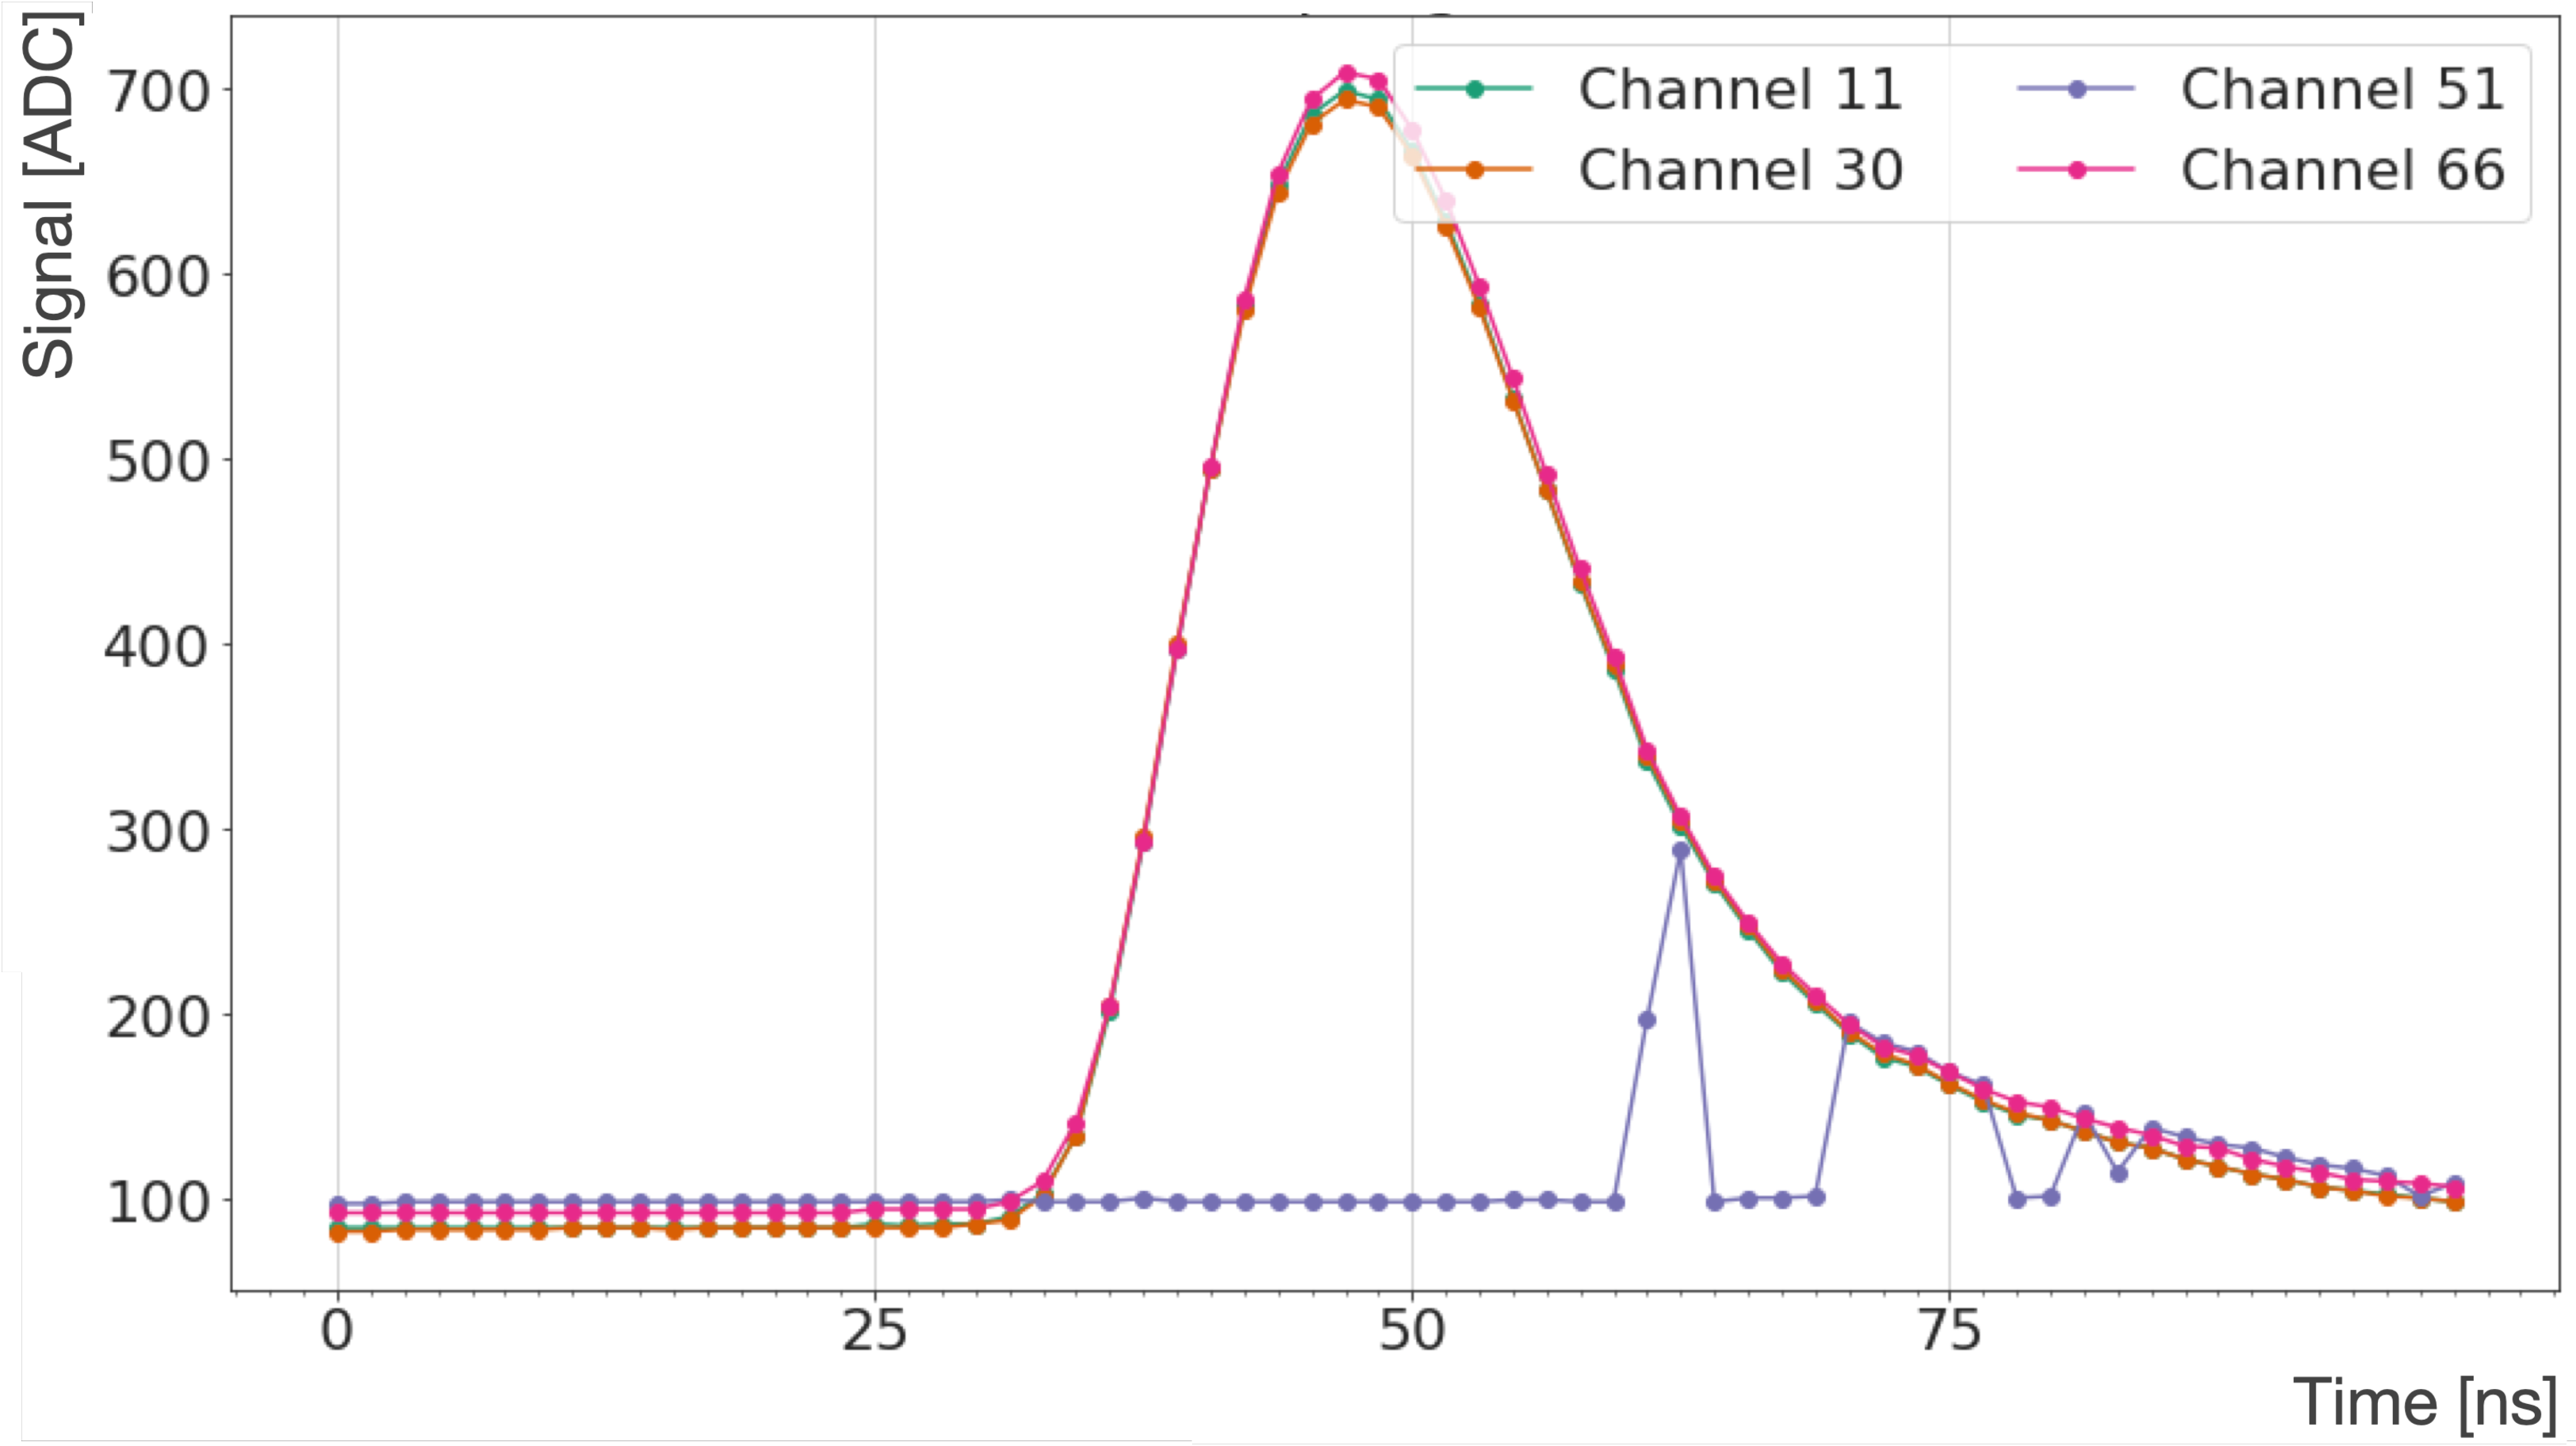
\includegraphics[height=0.25\linewidth]{Figures/HGCAL/ADCIssue_Median.pdf}
    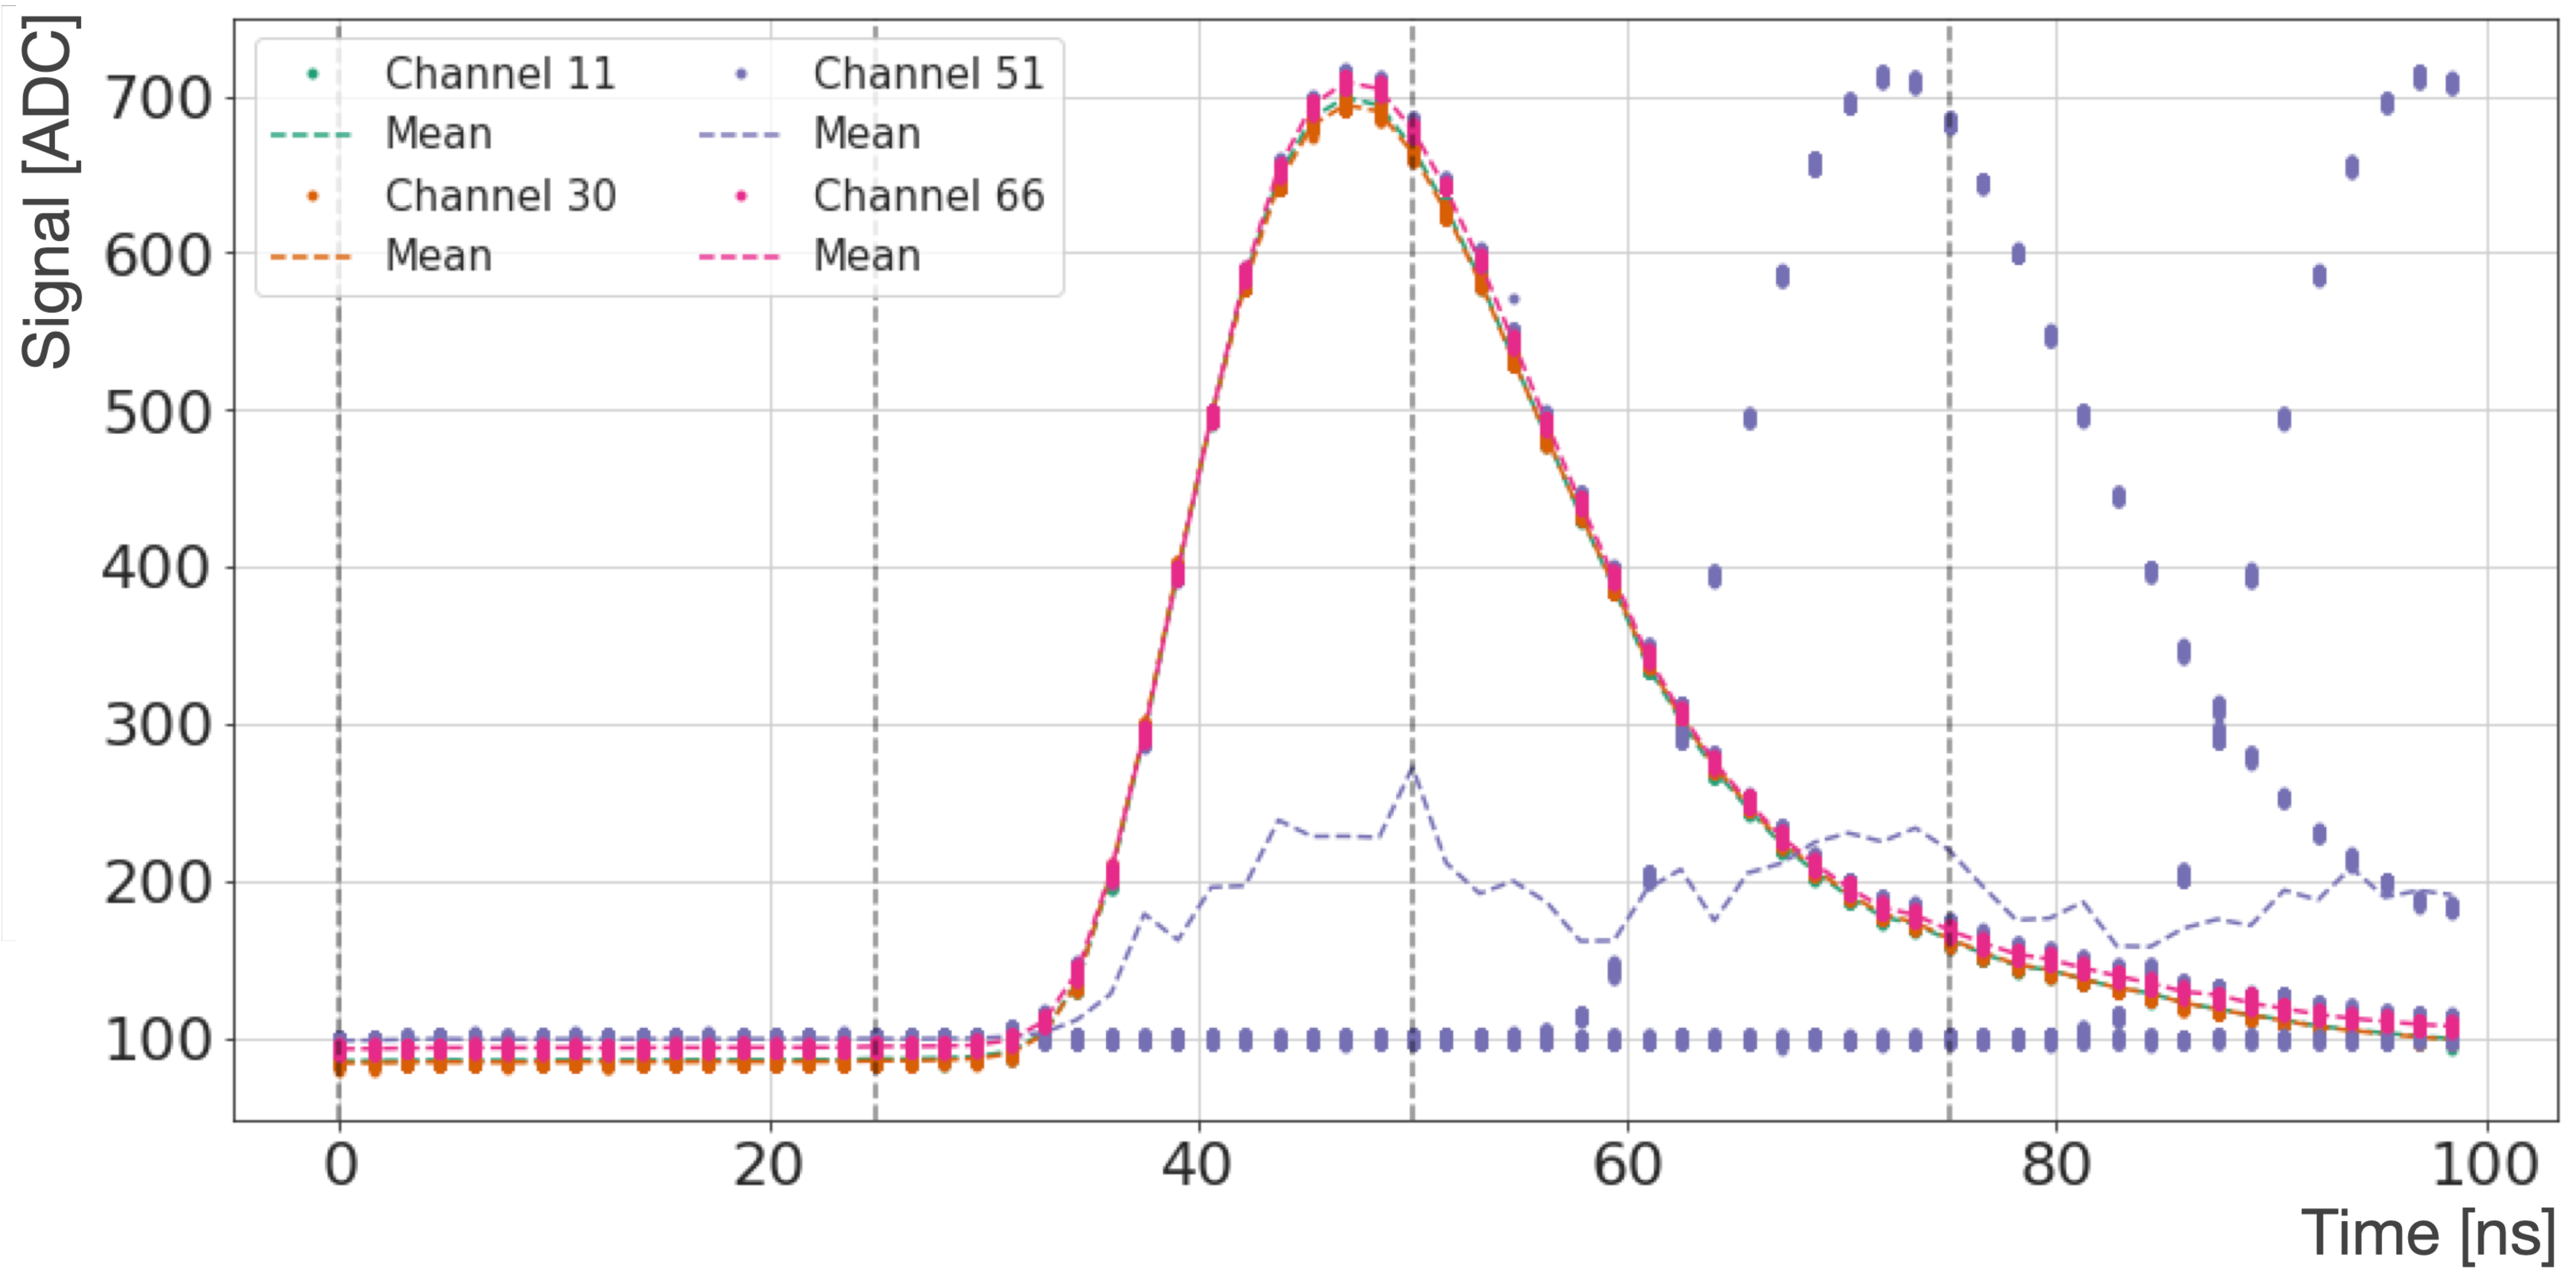
\includegraphics[height=0.25\linewidth]{Figures/HGCAL/ADCIssue_Raw.pdf}
    \caption{Example of data acquisition showing the issue in the ADC conversion: channels 11, 30, and 66 show the good expected performance, channel 51 shows unexpected behaviour. The left plot presents the previous testing procedure, reporting only the median value of multiple acquisitions. The right plot presents the updated testing procedure, revealing the signal reverberation caused by the ADC problem.}
    \label{fig:ADCIssue}
\end{figure}

The second issue is discovered in the ADC digitisation process. The identification of this anomaly has proven challenging, due to the employed data acquisition techniques: each data point representing the signal pulse is given by the median value derived from multiple acquisitions (typically 100, though the number is configurable). This methodology is necessary to estimate the impact of the electronic noise, which cannot be accurately assessed through a single injection.
With this data acquisition method, certain HGCROC3 prototypes exhibit inconsistent responses, confined to specific phases, as illustrated in the left plot of Figure~\ref{fig:ADCIssue}.

To elucidate the underlying cause of this behavior, individual injection events need to be examined. By analyzing each event separately, as depicted in the right plot of Figure~\ref{fig:ADCIssue}, it is possible to observe that certain events are inaccurately reconstructed in the wrong bunch crossing, leading to a signal reverberation shifted in time. The median value is anomalously influenced only during specific phases, depending on the number of misreconstructed events.
Since the existing testing method cannot detect the issue, the procedure is updated to represent all events independently. This revision reveals the presence of numerous channels afflicted by the same issue.

\bigbreak

Extensive investigations have been undertaken to determine the specific component responsible for this anomaly. 
Various tests have been executed to discern whether the issue was related to the chip architecture or to external factors.
The analysis reveals that the anomaly exhibits dependency on both the conversion delay time and the operational temperature, as demonstrated in Figures~\ref{fig:ADCIssue_Delay} and ~\ref{fig:ADCIssue_Temperature}. 
However, even the minimum delay time and the reduced temperature of $-30^\circ$C fail to fully mitigate the issue across all channels, as each channel responds differently to delay and temperature changes. 
Given the significant impact of this issue on the chip performance, the ADC conversion circuit of the HGCROC3 has been revised to strengthen the conversion and avoid the signal reverberation.
An updated chip version, incorporating these corrections along with other necessary fixes, has been submitted to the manufacturers in May 2024.

\begin{figure}
    \centering
    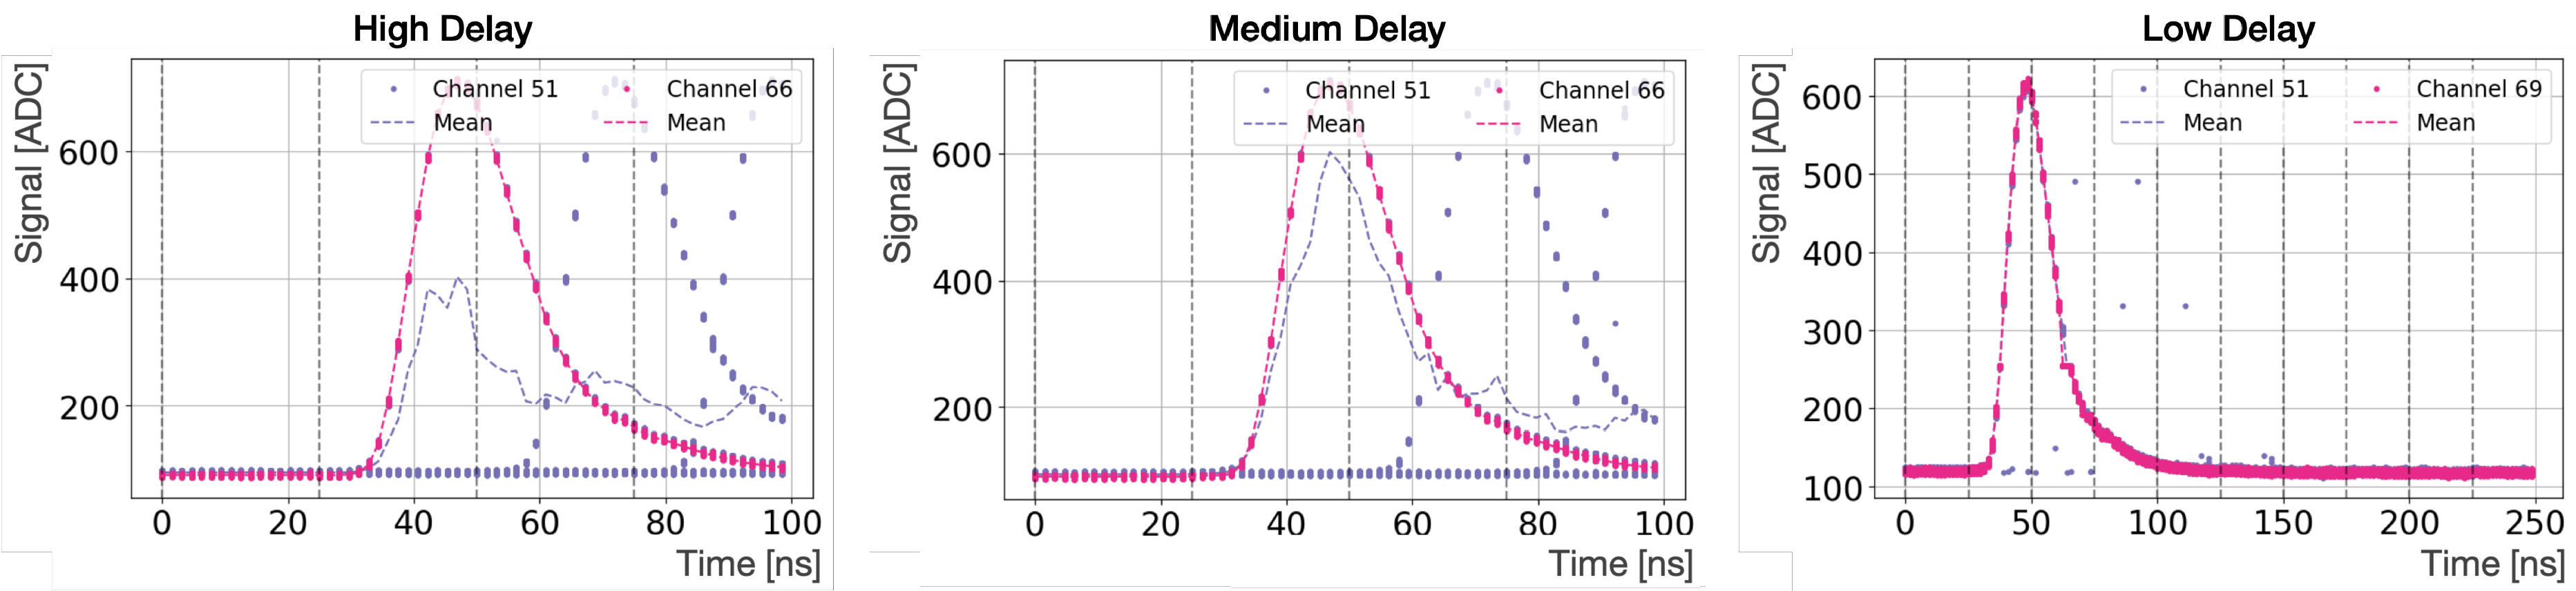
\includegraphics[width=0.99\linewidth]{Figures/HGCAL/ADCIssue_Delay.pdf}
    \caption{Dependency of the issue in the ADC conversion on the delay time for the conversion, configurable as a I2C parameter in the HGCROC3. The problematic channel 51 shows better performance for faster conversion times, but even the minimum delay time is not enough to entirely cancel the reverberation.}
    \label{fig:ADCIssue_Delay}
\end{figure}

\begin{figure}
    \centering
    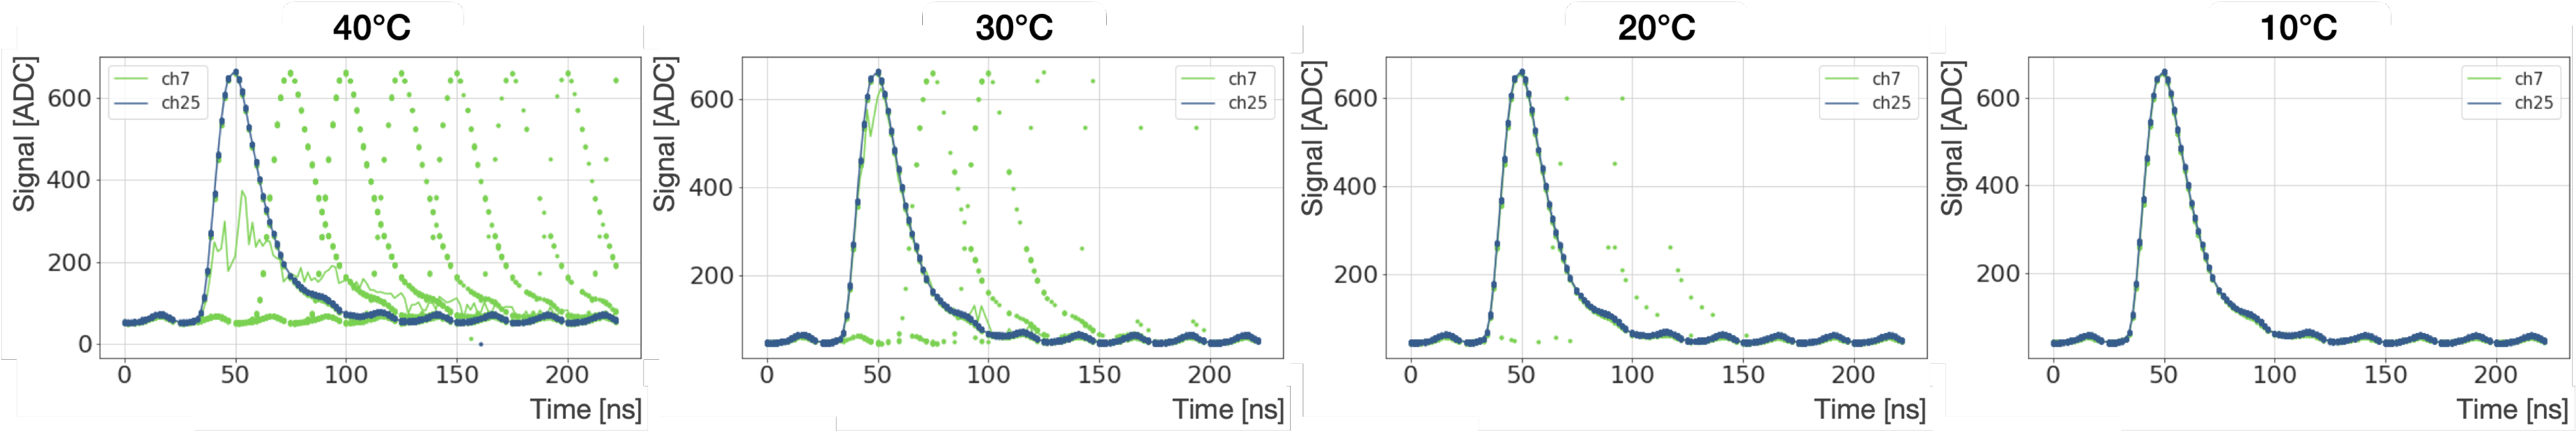
\includegraphics[width=0.99\linewidth]{Figures/HGCAL/ADCIssue_Temperature.pdf}
    \caption{Dependency of the issue in the ADC conversion on the temperature. The performance of the problematic channel 7 gradually improves with lower temperature and is completely restored when reaching $10^{\circ}$C.}
    \label{fig:ADCIssue_Temperature}
\end{figure}

\begin{figure}
    \centering
    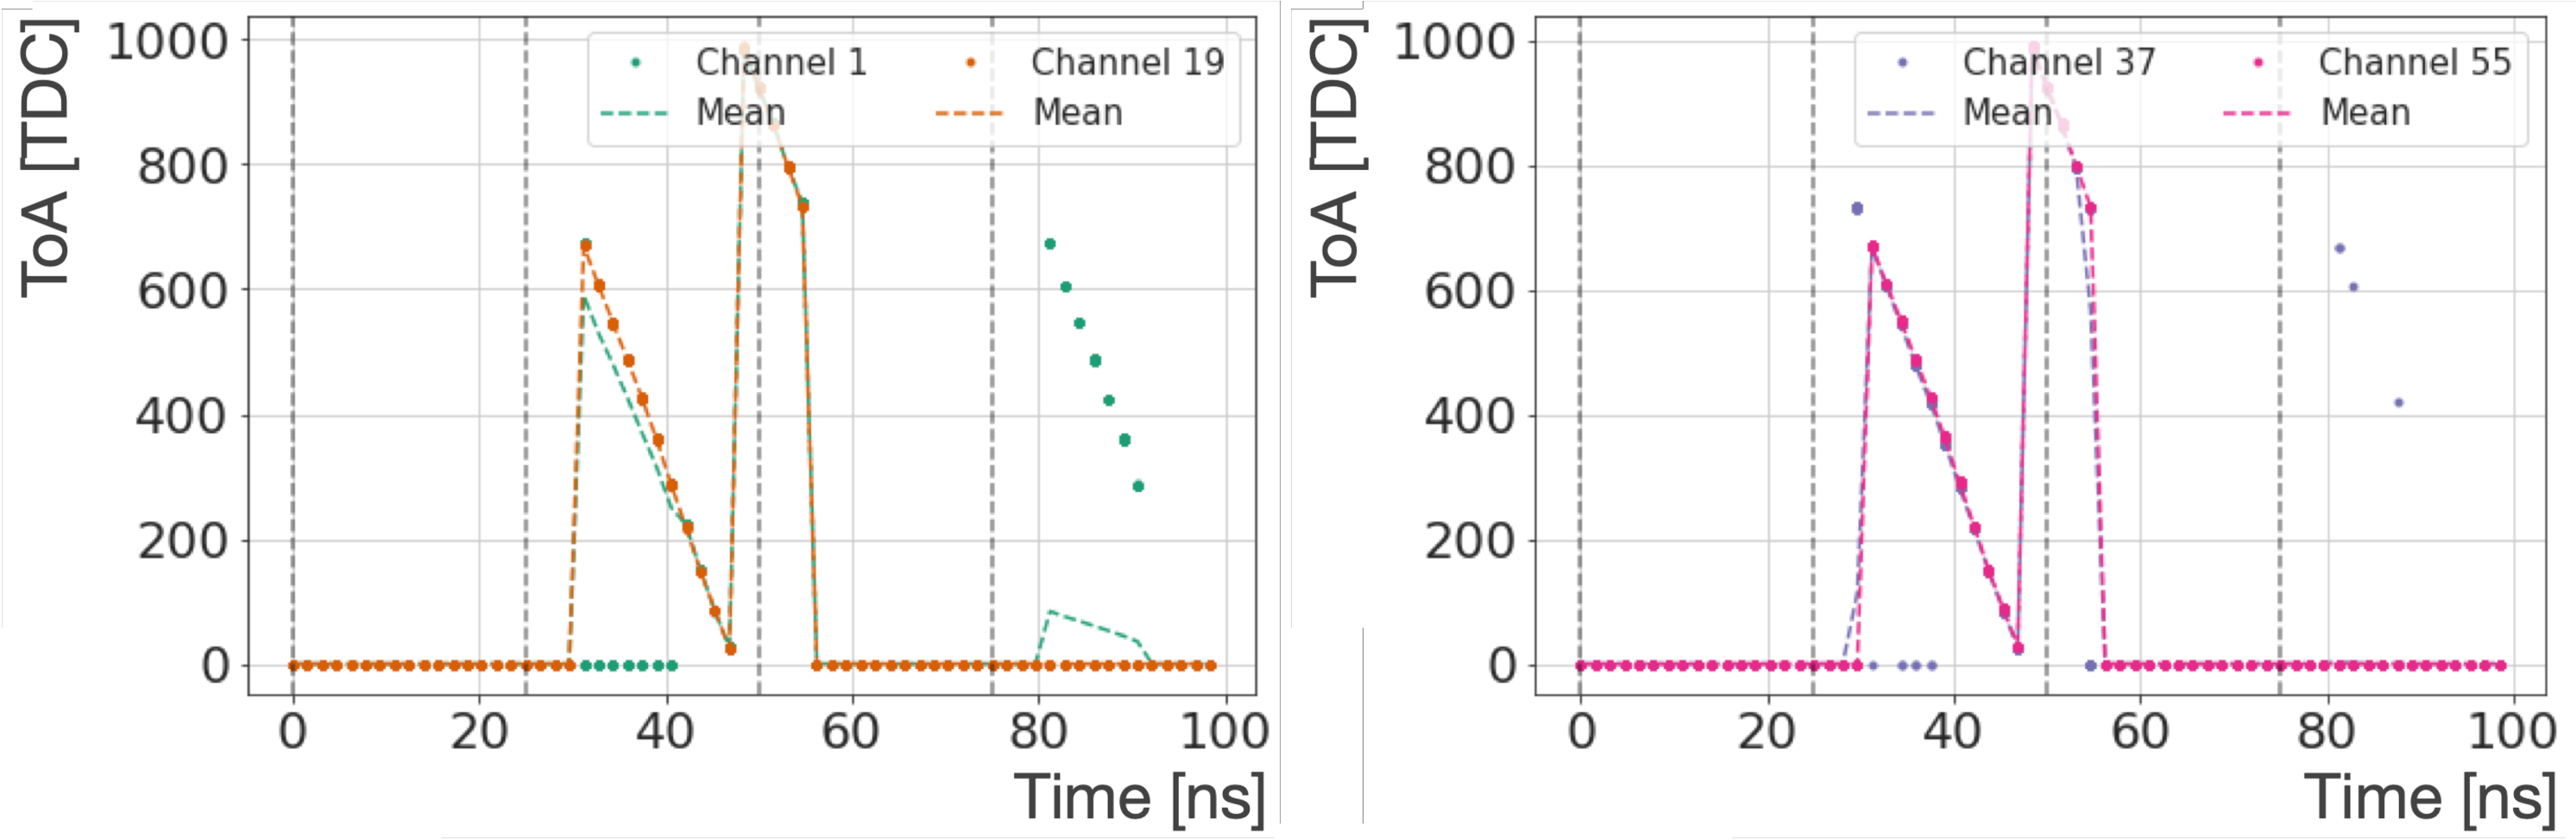
\includegraphics[width=0.8\linewidth]{Figures/HGCAL/TDCIssue.pdf}
    \caption{Example of data acquisition showing the issue in the TDC conversion: channels 19 and 55 show the good expected performance, channels 1 and 37 show unexpected behaviour, only visible by looking at the single events with the updated testing procedure.}
    \label{fig:TDCIssue}
\end{figure}

\subsubsection{Issue in TDC conversion}
\label{subsubsec:Issue in TDC conversion}

The new testing procedure has also led to the discovery of another issue in the conversion block of the TDC component, affecting the digitisation of the ToA and ToT values. 
An example of the anomalous behaviour is reported in Figure~\ref{fig:TDCIssue}. At a first glance, the manifestation appears analogous to that of the ADC conversion, with a reverberation of the signal in the incorrect bunch crossing period. However, a closer analysis reveals that the ToA measurement is correctly performed, but transmitted in the wrong bunch crossing. 
This behavior is linked to a metastability of the digitisation circuit in assigning the TDC information to the correct bunch crossing. The problem has been reproduced in the simulations and can be rectified through a slight modification of the TDC conversion circuit.

\bigbreak

A revised design of the chip, allowing the ADC and TDC conversion problems to be fixed, has been implemented in the new ASIC version, HGCROC3b. 

%%%%%%%%%%%%%%%%%%%%%%%%%%%%%%%%%%%%%%%%%%%%%%%%%%%%%%%%%%%%%%%%%%%%%%%%%%%%%%%%%%%%%%%%%%%%
%%%%%%%%%%%%%%%%%%%%%%%%%%%%%%%%%%%%%%%%%%%%%%%%%%%%%%%%%%%%%%%%%%%%%%%%%%%%%%%%%%%%%%%%%%%%
%%%%%%%%%%%%%%%%%%%%%%%%%%%%%%%%%%%%%%%%%%%%%%%%%%%%%%%%%%%%%%%%%%%%%%%%%%%%%%%%%%%%%%%%%%%%
%%%%%%%%%%%%%%%%%%%%%%%%%%%%%%%%%%%%%%%%%%%%%%%%%%%%%%%%%%%%%%%%%%%%%%%%%%%%%%%%%%%%%%%%%%%%

\section{Irradiation testing of the HGCROC3}
\label{sec:The HGCROC3 irradiation testing}

Once mounted on the HGCAL detector, the HGCROC3 will encounter the extremely harsh radiation environment of the CMS forward region. According to FLUKA \cite{Fassò:277533} simulations, the HGCAL front-end electronics will be subjected to a hadron flux up to $3.5\times10^6\,\textrm{s}^{-1}\,\textrm{cm}^{-2}$, with a total absorbed dose of approximately $200\,\textrm{Mrad}$ after the expected 10-year lifetime of the detector. 
The results of the FLUKA simulations, in terms of expected flux and integrated dose, are illustrated in Figure~\ref{fig:HGCALDose}. The high pseudorapidity regions of the detector, situated very close to the beam line, are predicted to experience the highest fluence, reaching up to $10^{16}\,\textrm{n}_{\textrm{eq}}\,\textrm{cm}^{-2}$.

\bigbreak

An essential step in the design validation of HGCROC3 is to test and quantify potential alterations in its performance under radiation exposure.
Radiation can severely impact electronics, causing memory errors, increased leakage currents, and in extreme cases, complete loss of functionality. These effects are a reliability concern not only in high-energy physics experiments, but also in long-term space missions, where devices endure prolonged exposure to Galactic Cosmic Radiation (GCR).

Radiation effects on electronic devices are traditionally categorised into two main categories:
\begin{itemize}
    \item [-] the Total Integrated Dose (TID) effects are a cumulative long-term degradation of the device due to prolonged exposure to ionizing radiation,
    \item [-] the Single Event Effects (SEE) are instantaneous device failures that can occur at any moment in a high-energy radiation environment, typically caused by direct interaction of particles with the device material.
\end{itemize}

\begin{figure}
    \centering
    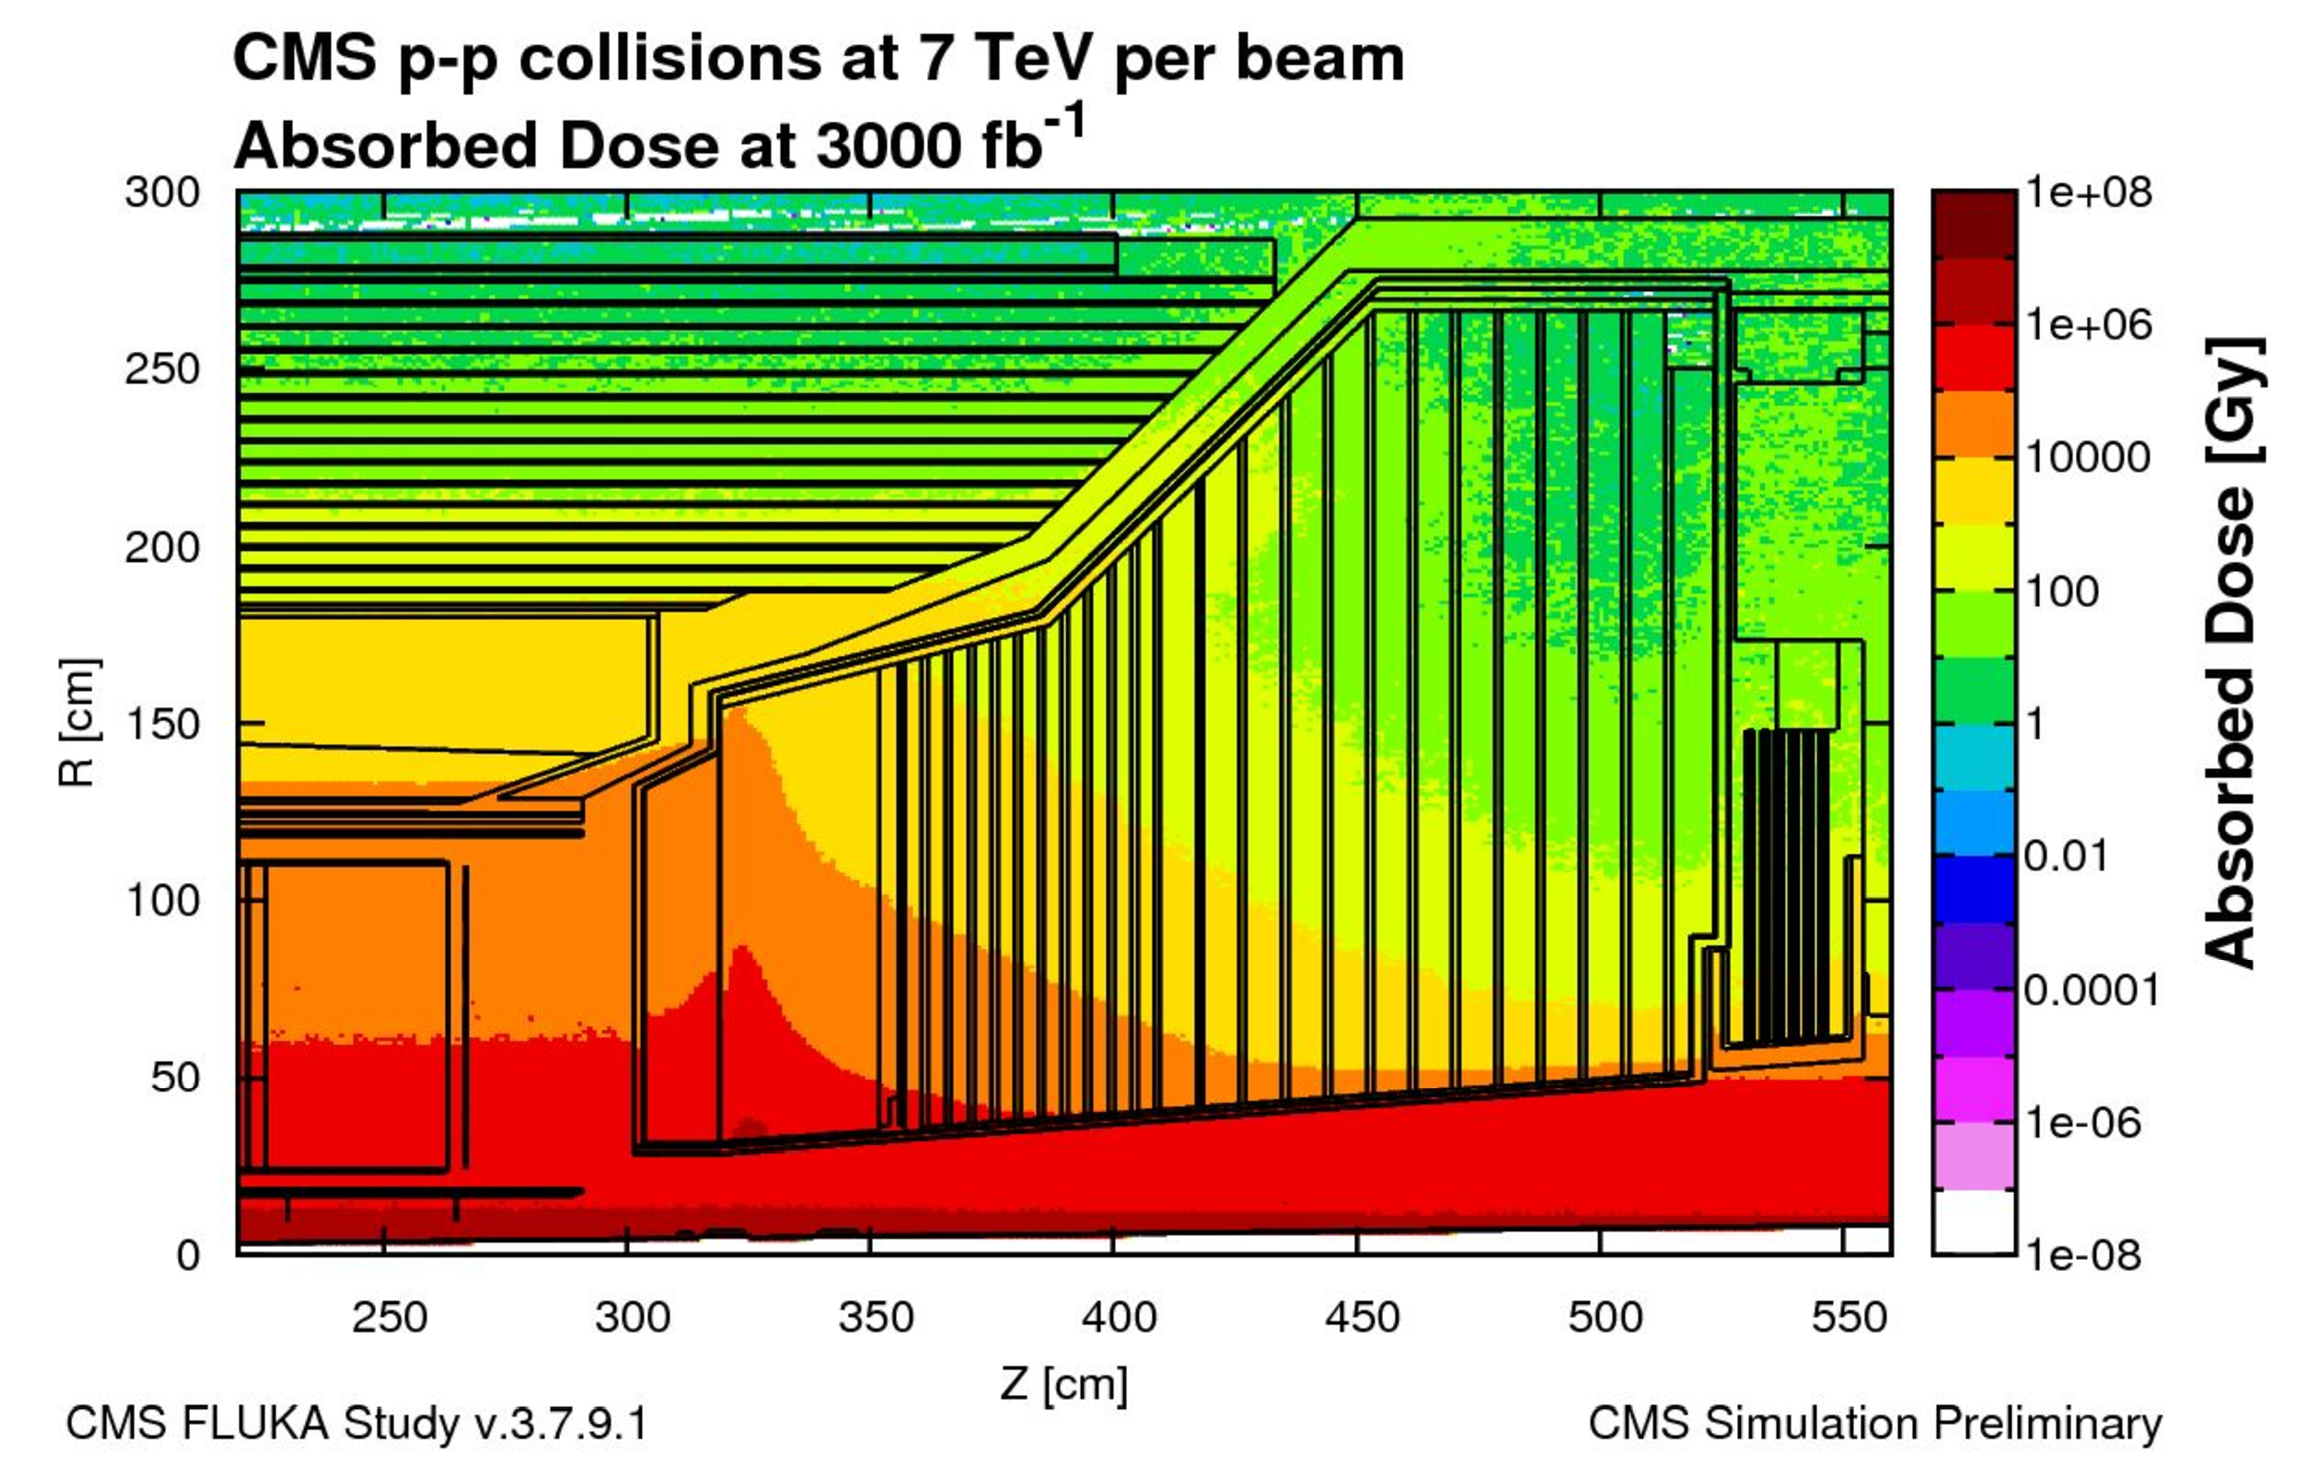
\includegraphics[width=0.49\linewidth]{Figures/HGCAL/HGCALDose.pdf}
    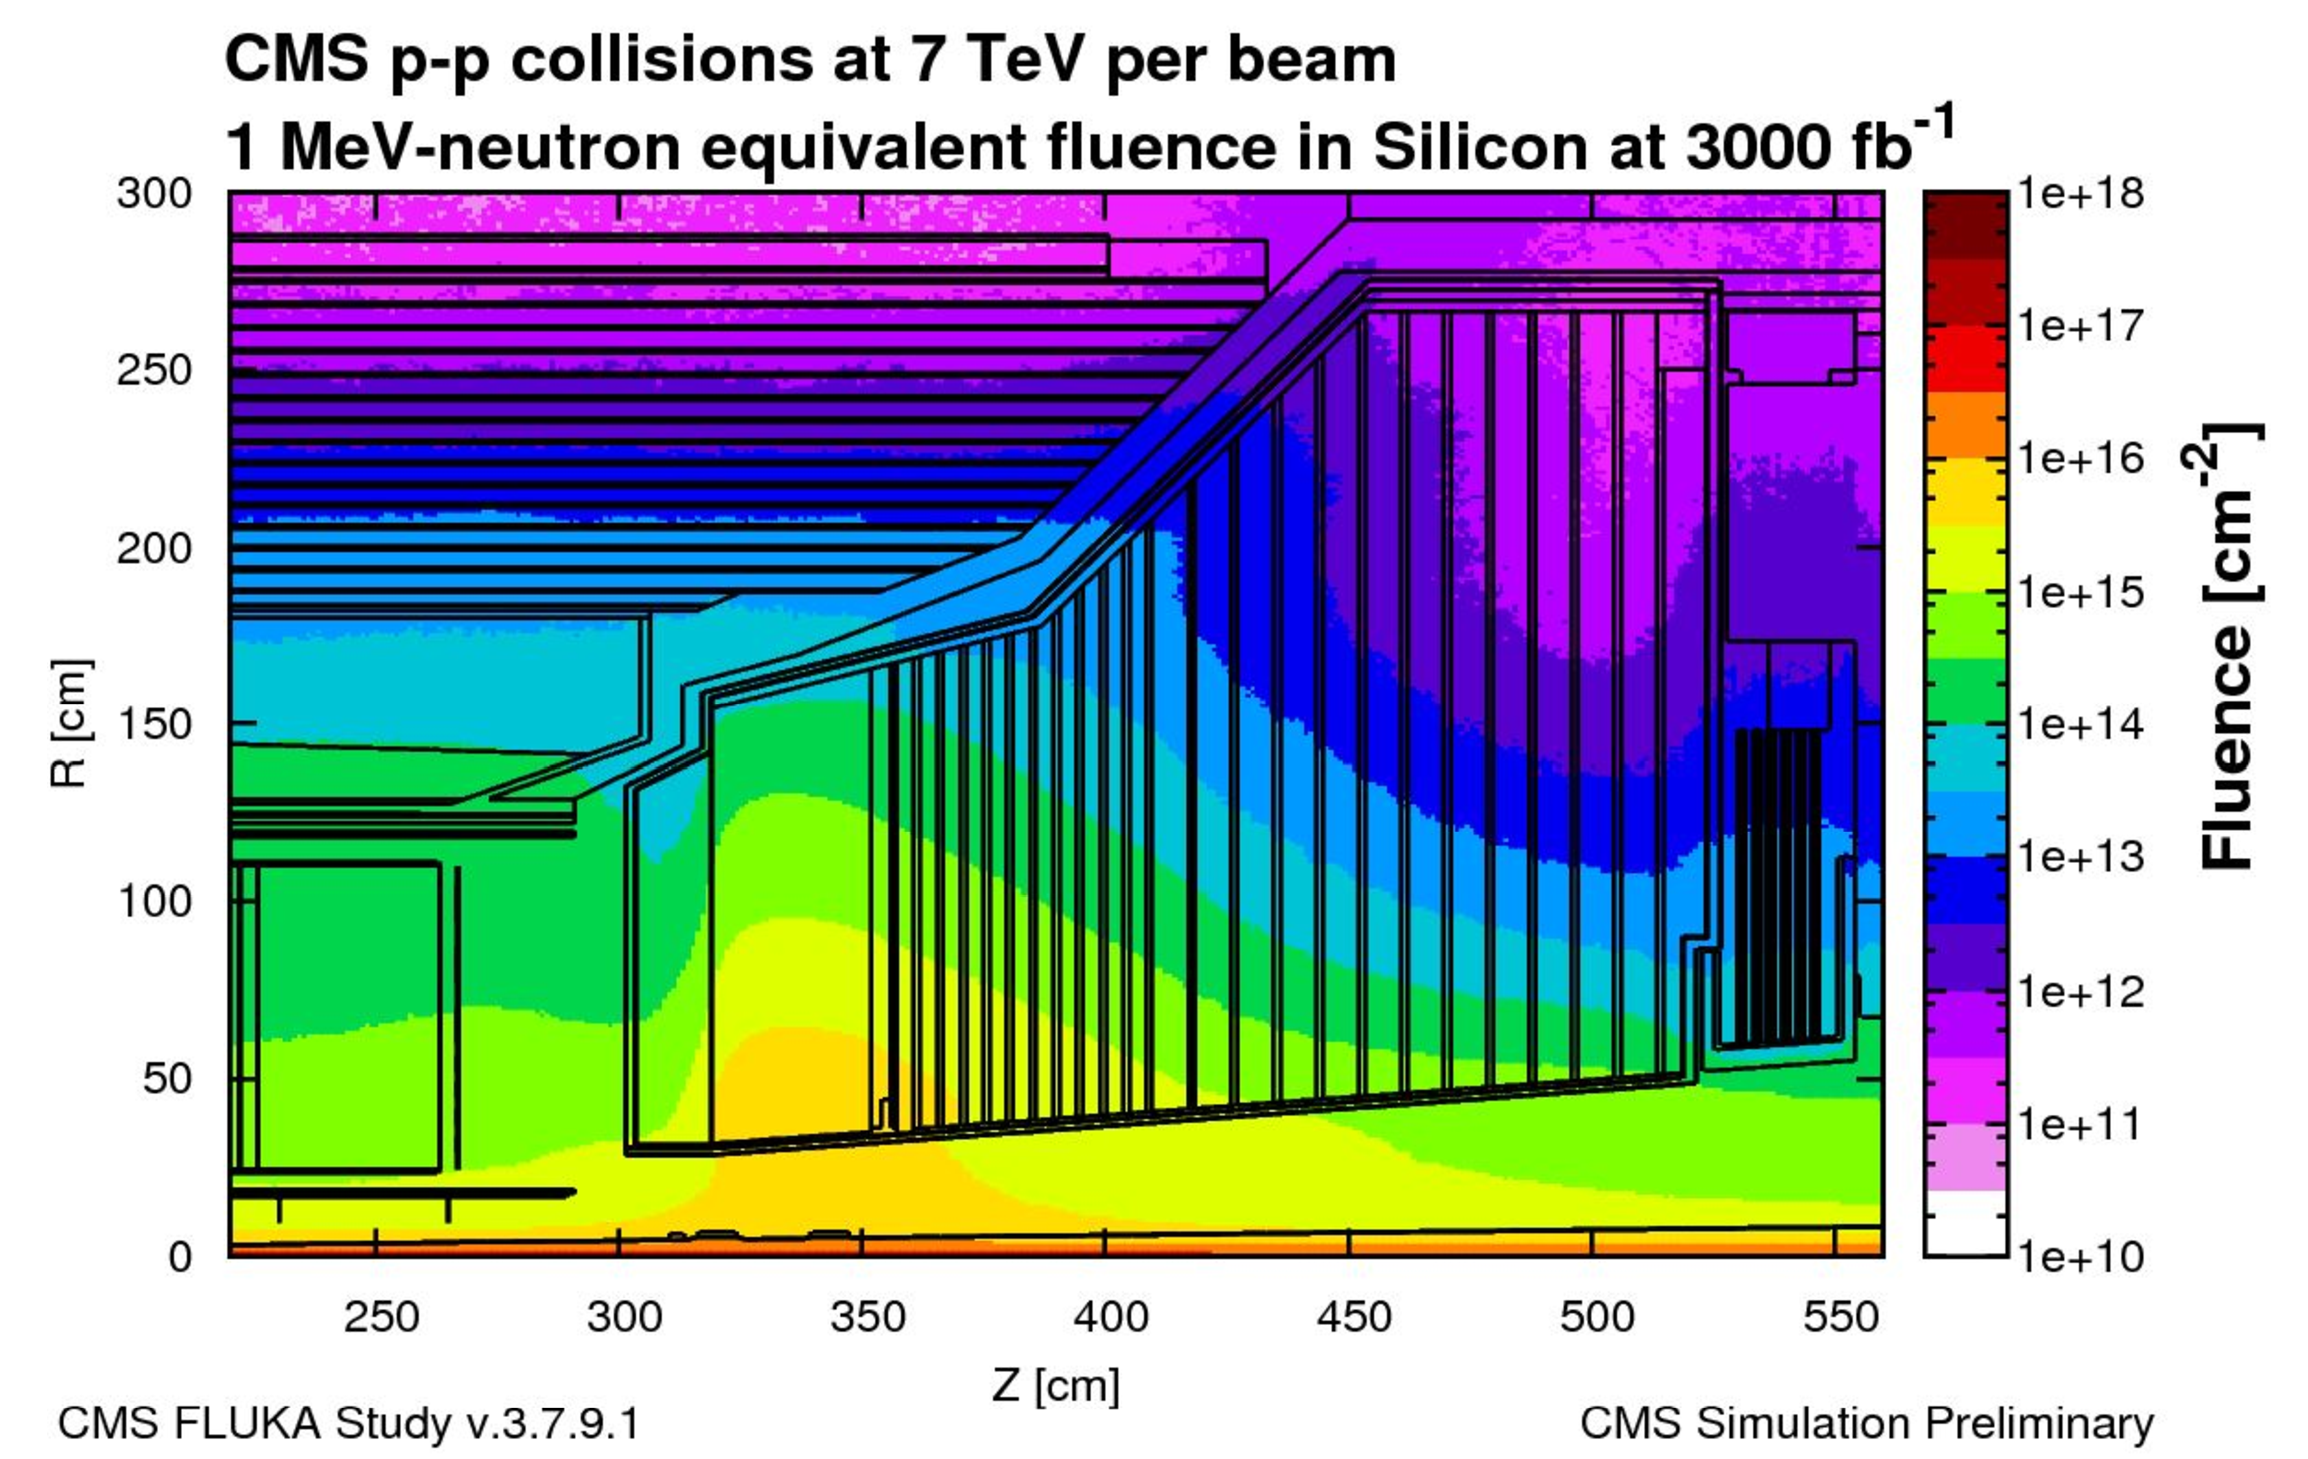
\includegraphics[width=0.49\linewidth]{Figures/HGCAL/HGCALFlux.pdf}
    \caption{Simulated dose (left) and fluence (right) of ionizing radiation accumulated in the HGCAL detector after an integrated luminosity of 3000 $\textrm{fb}^{-1}$, simulated using the FLUKA program, and shown as a two-dimensional map in the radial and longitudinal coordinates, $r$ and $z$.}
    \label{fig:HGCALDose}
\end{figure}

The TID accumulated radiation damage typically impacts analog electronics more severely, with a lesser impact on digital memories or data processing components. After irradiation, a self-healing process known as \textit{annealing} can occur over time, gradually repairing these malfunctions.
In contrast, the SEE irradiation predominantly affects the digital part of the device, potentially leading to memory alterations and data transfer issues.

\bigbreak

The radiation hardness of modern electronic devices, particularly their resistance to both TID and SEE, is crucial for ensuring long-term reliability. The following sections describe the irradiation campaigns conducted on the HGCROC3 to assess potential TID and SEE effects, and verify its radiation hardness.

%%%%%%%%%%%%%%%%%%%%%%%%%%%%%%%%%%%%%%%%%%%%%%%%%%%%%%%%%%%%%%%%%%%%%%%%%%%%%%%%%%%%%%%%%%%%
%%%%%%%%%%%%%%%%%%%%%%%%%%%%%%%%%%%%%%%%%%%%%%%%%%%%%%%%%%%%%%%%%%%%%%%%%%%%%%%%%%%%%%%%%%%%
%%%%%%%%%%%%%%%%%%%%%%%%%%%%%%%%%%%%%%%%%%%%%%%%%%%%%%%%%%%%%%%%%%%%%%%%%%%%%%%%%%%%%%%%%%%%
%%%%%%%%%%%%%%%%%%%%%%%%%%%%%%%%%%%%%%%%%%%%%%%%%%%%%%%%%%%%%%%%%%%%%%%%%%%%%%%%%%%%%%%%%%%%

\section{Total Integrated Dose campaigns}
\label{sec:Total Integrated Dose} 

The Total Integrated Dose (TID) irradiation test aims at evaluating the cumulative radiation damage induced by ionizing particles on the HGCROC3, and at proving its radiation tolerance up to $200\,\textrm{Mrad}$. By reproducing the long-term effects of radiation exposure, the TID test identifies potential vulnerabilities in the device design and functionality.

\bigbreak

The first TID campaign on the HGCROC3 is performed at the Obelix facility (CERN) using a 10~keV X-ray beam. The experimental set-up is illustrated in Figure~\ref{fig:TID_Setup}.
The X-ray machine is placed inside a chamber for both radiation shielding and better humidity control, to prevent condensation when operating the electronics at temperatures below $0^{\circ}$C. 
The prototype of the HGCROC3 is mounted on a mezzanine board and thinned from its original thickness of $250\,\mu\textrm{m}$ to $70\,\mu\textrm{m}$, for a better X-ray penetration.
The cooling system is configured with a copper plaque adhering to the mezzanine board, and two resistive sensors are placed close to the device to monitor temperature stability.

\bigbreak

Studies have shown that the radiation damage caused by ionizing particles is dependent on both temperature and dose rate~\cite{giulio}.
\begin{itemize}
    \item [-] Irradiation has a more significant impact at higher temperatures.  Ideally, the TID irradiation test should be performed at the expected HGCAL operating temperature of $-30^{\circ}$C; however such a low temperature is hardly reached by the available experimental set-up, consequently this campaign provides a worst-case scenario. 
    \item [-]  Additional radiation damage can arise at low dose rates. However, reaching the final dose of $200\,\textrm{Mrad}$ with the expected HL-LHC dose rate of $\sim10^2$~$\textrm{rad/h}$ would be hardly reproducible in a testing campaign. For this reason, a margin of at least +$50\%$ on the total injected dose should be considered during the irradiation testing at higher dose rates to account for this difference. 
\end{itemize}

During the HGCROC3 TID irradiation campaign, the chip is operated at $-10^{\circ}$C, the minimum temperature available for the experimental set-up, and the dose rate is set to the highest possible value of $2.45\,\textrm{Mrad/h}$, in order to complete the test within the available one-week time frame. 
To account for the different dose rate with respect to the HL-LHC conditions, a +$75\%$ margin is considered in addition the the total expected dose of $200\,\textrm{Mrad}$.
At the end of the TID radiation exposure, the total integrated dose delivered to the HGCROC3 is $345\,\textrm{Mrad}$.

\bigbreak

During the exposure time, the performance of the HGCROC3 is continuous monitored in terms of power consumption, ADC and TDC measurements. The results are described in the following paragraphs. 

\begin{figure}
    \centering
    \includegraphics[height=0.32\linewidth]{Figures/HGCAL/TID_Setup1.pdf}
    \includegraphics[height=0.32\linewidth]{Figures/HGCAL/TID_Setup2.pdf}
    \caption{The experimental set-up for the TID irradiation campaign performed at the Obelix facility (CERN). On the left, a picture of the X-ray machine, located above the mezzanine board hosting the HGCROC3 prototype; the FPGA board is located away from the X-ray beam to protect it from radiation damage. On the right, a close-up on the mezzanine board hosting the HGCROC3, tightly fixed through a white plastic support to the cooling system plaque underneath; the copper tubes connected to the cooling system and the resistive temperature sensors are also visible.}
    \label{fig:TID_Setup}
\end{figure}

\subsection{Effects on the ADC and TDC performance}
\label{subsec:ADC and TDC performance}

During the TID radiation exposure, no impact on the charge or time measurements and no misbehaviour in the DRAMs is observed. The ADC and TDC performance against injected charge after irradiation remains consistent with pre-irradiation conditions.
Figure~\ref{fig:TID_SignalShape} and~\ref{fig:TID_ADCLinearity} show the comparison of the ADC performance before and after radiation exposure: the recorded signal shape does not show any degradation, and the rising and falling edge time constants are unaffected. Additionally, the recorded signal amplitude maintains the expected linear dependency on the injected input charge.
Figure~\ref{fig:TID_TimeWalk} presents the comparison of the TDC performance on the ToA measurement before and after radiation exposure, showing no degradation in the TDC component.

\begin{figure}
    \centering
    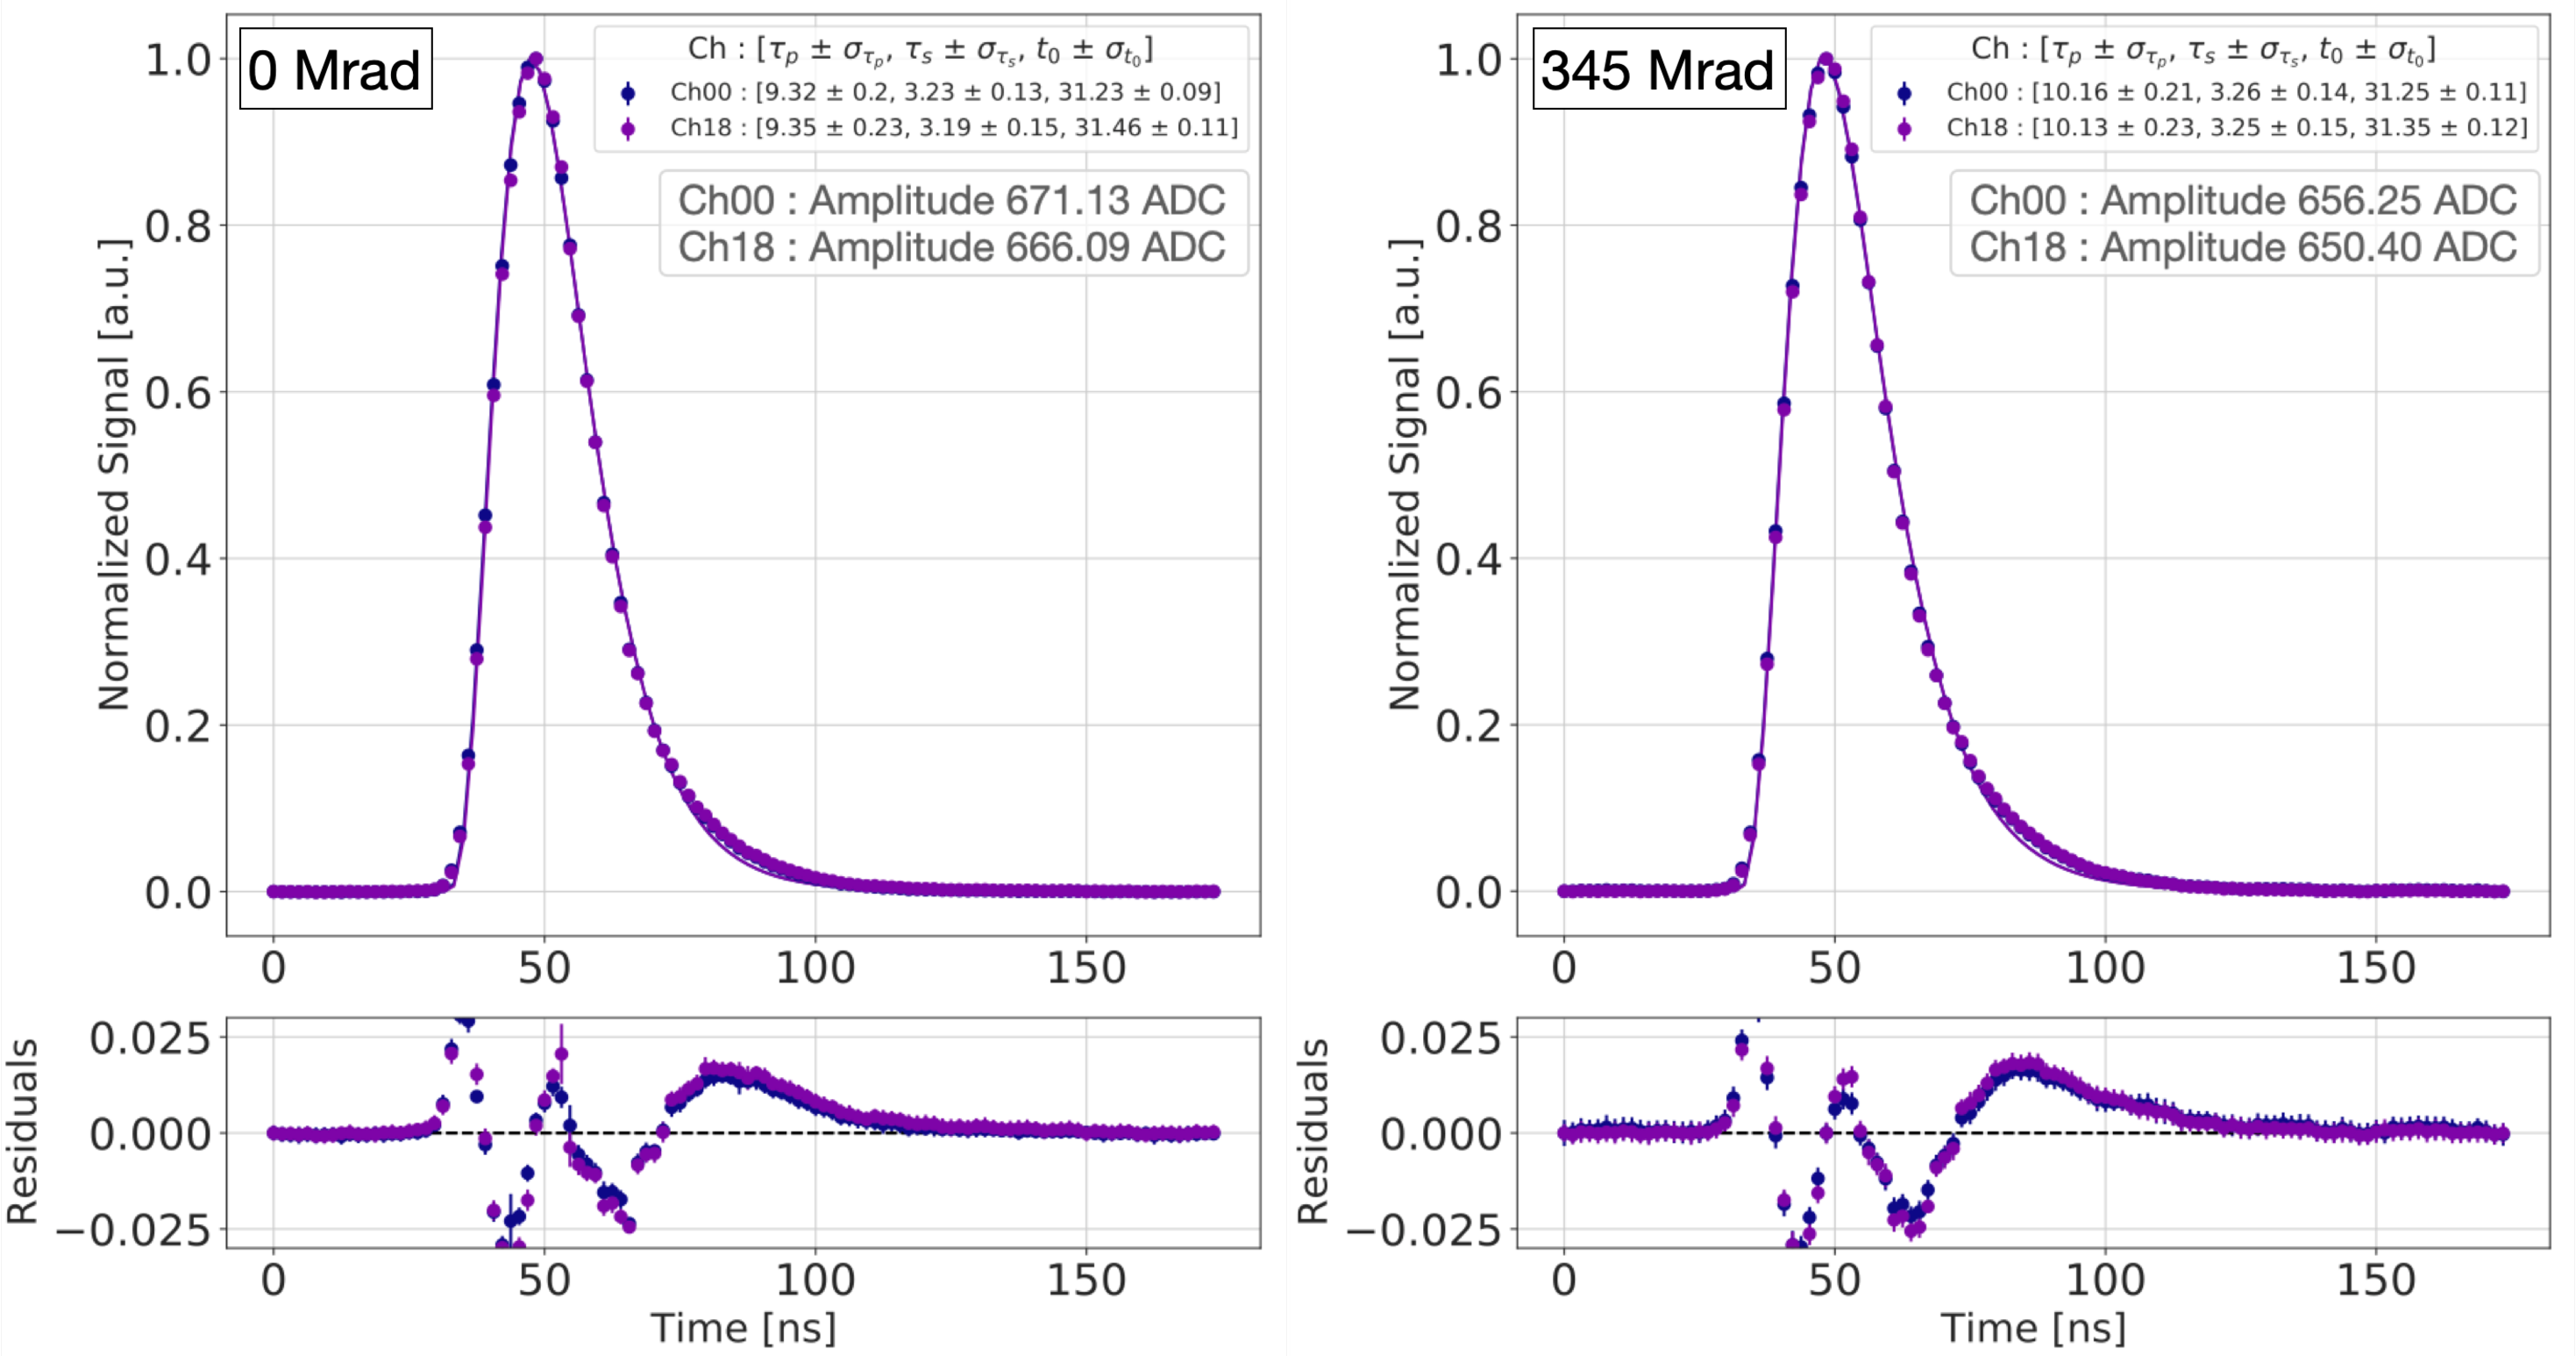
\includegraphics[width=0.7\linewidth]{Figures/HGCAL/TID_SignalShape.pdf}
    \caption{Normalised signal pulse recorded by 2 exemplary channels at the beginning (left) and at the end of the TID irradiation campaign. No degradation is observed in the signal shape, the rising and falling edge characteristic times don't show any significant variation.}
    \label{fig:TID_SignalShape}
\end{figure}

\begin{figure}
    \centering
    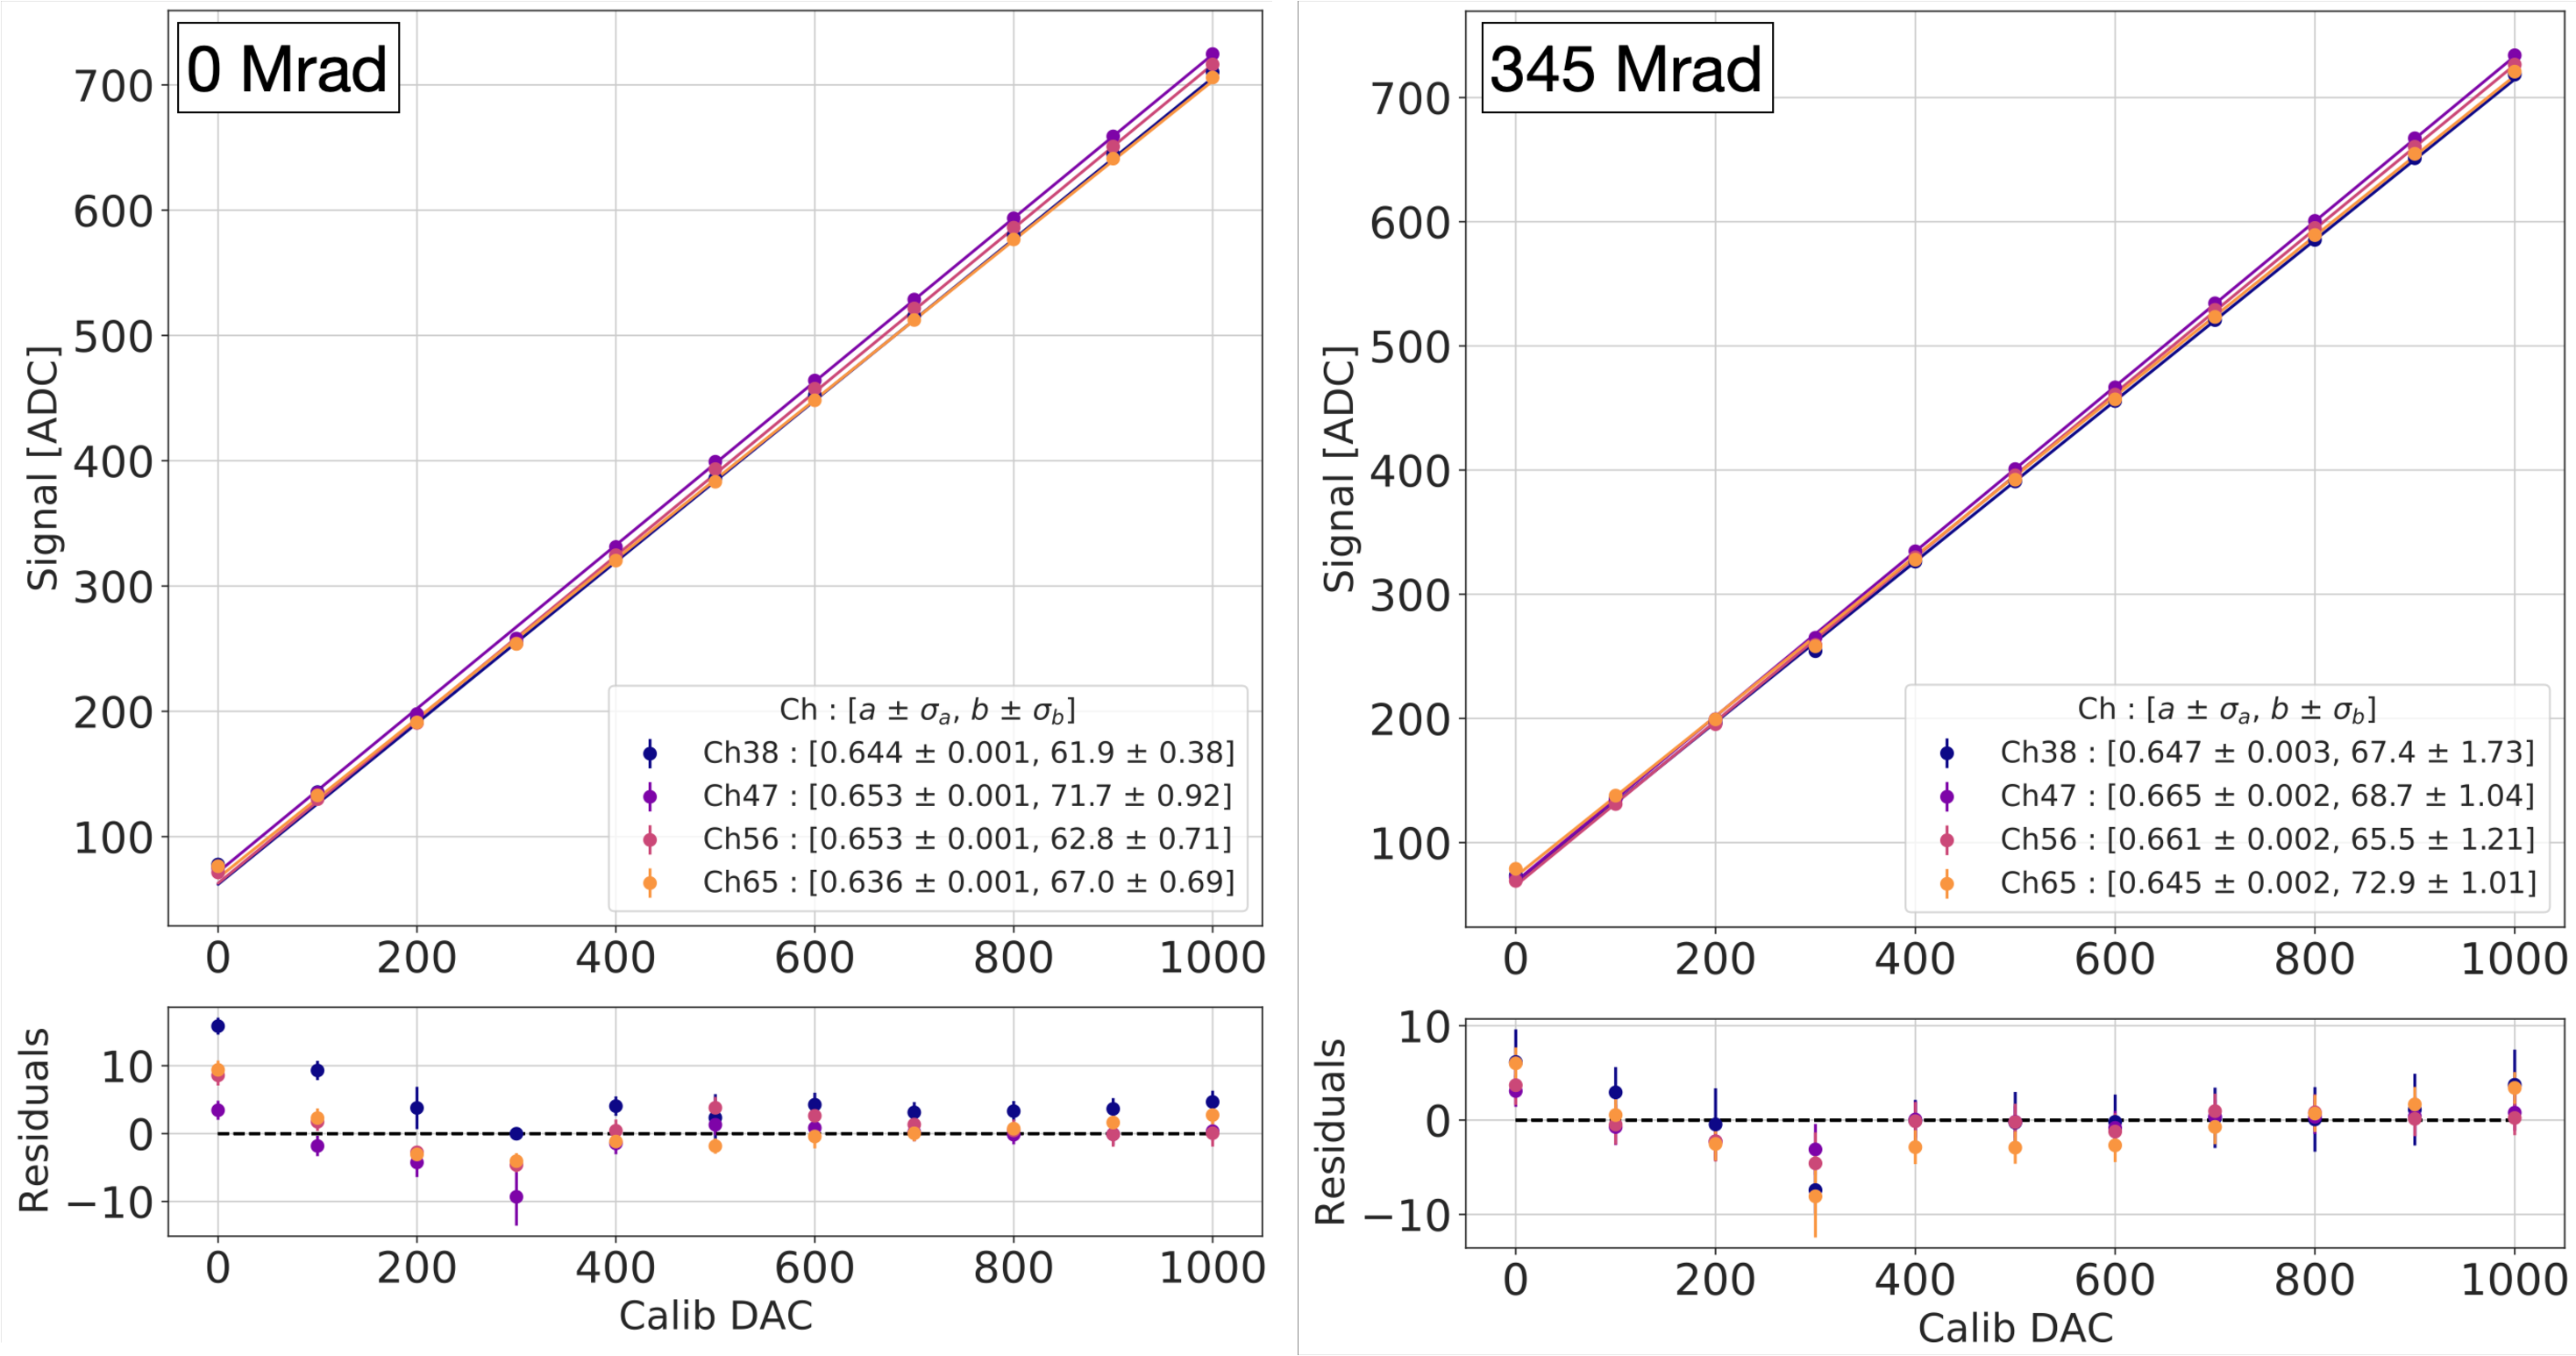
\includegraphics[width=0.7\linewidth]{Figures/HGCAL/TID_ADCLinearity.pdf}
    \caption{Linear dependence of the measured signal amplitude on the injected input charge parameter \texttt{Calib\_DAC} for 4 representative channels of the HGCROC3 at the beginning (left) and at the end (right) of the TID irradiation campaign.}
    \label{fig:TID_ADCLinearity}
\end{figure}

\begin{figure}
    \centering
    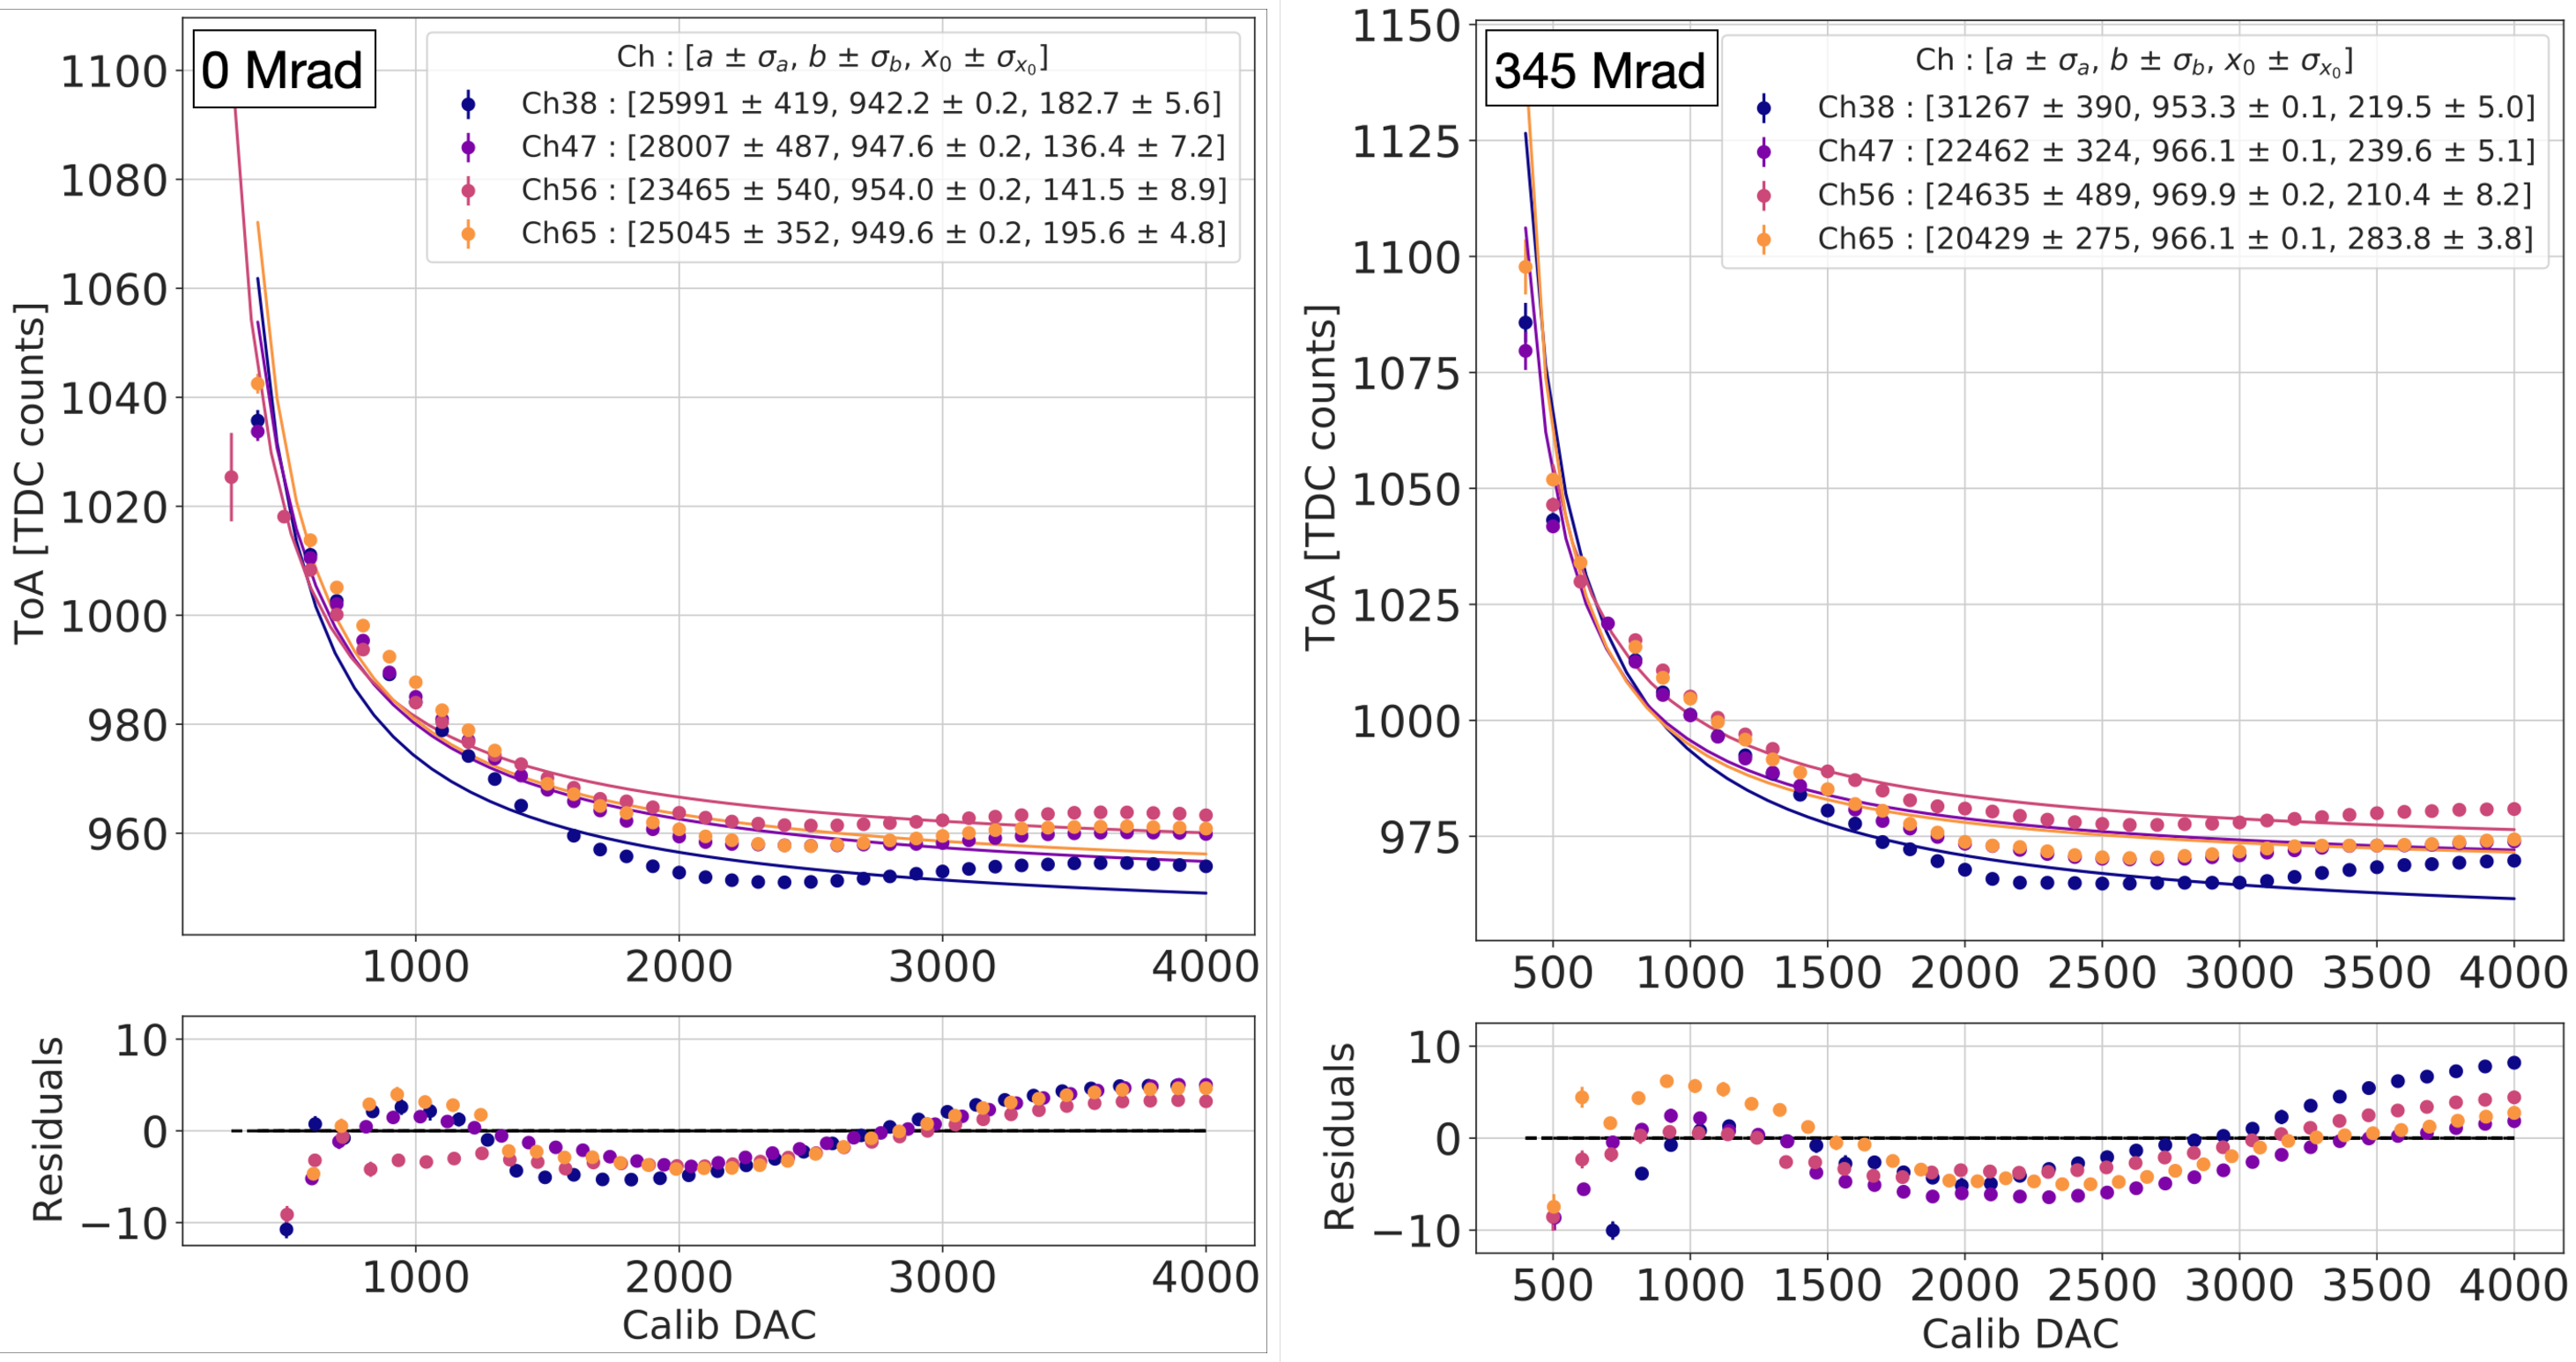
\includegraphics[width=0.7\linewidth]{Figures/HGCAL/TID_TimeWalk.pdf}
    \caption{Time walk curve for the ToA as a function of the injected input charge parameter \texttt{Calib\_DAC} for 4 representative channels of the HGCROC3 at the beginning (left) and the end (right) of the irradiation.}
    \label{fig:TID_TimeWalk}
\end{figure}

\bigbreak

The TID radiation leads to performance degradation in terms of electronic noise: a +$20\%$ increase in the noise is observed at the end of the exposure. Figure~\ref{fig:TID_Noise} shows the distribution of the preamplifier noise for the 72 normal channels of the HGCROC3 at the beginning and at the end of the TID irradiation campaign: from an initial value of 1.4~ADC counts, the noise mean reaches 1.75~ADC counts after $345\,\textrm{Mrad}$ dose. 

The noise increase can significantly impact the HGCROC3 performance, reducing the precision of both the ADC and TDC measurements, and affecting the particle reconstruction capabilities. This effect will sum up to the evolution of the silicon sensor noise during radiation exposure and needs to be accounted for in the simulation of the end-of-life detector performance.

% The evolution of the preamplifier noise distribution for the 72 channels of the HGCROC3 is shown in Figure~~\ref{fig:noiseevolution} as a function of the injected dose. A +$20\%$ increase - from 1.5 to 1.8 ADC counts - of the noise mean after $345\,\textrm{Mrad}$ dose is observed, with a -$5\%$ recovery already after 12 hours of annealing. Further studies will be conducted to simulate the effects of the annealing taking place in between consecutive data taking runs.

\begin{figure}
    \centering
    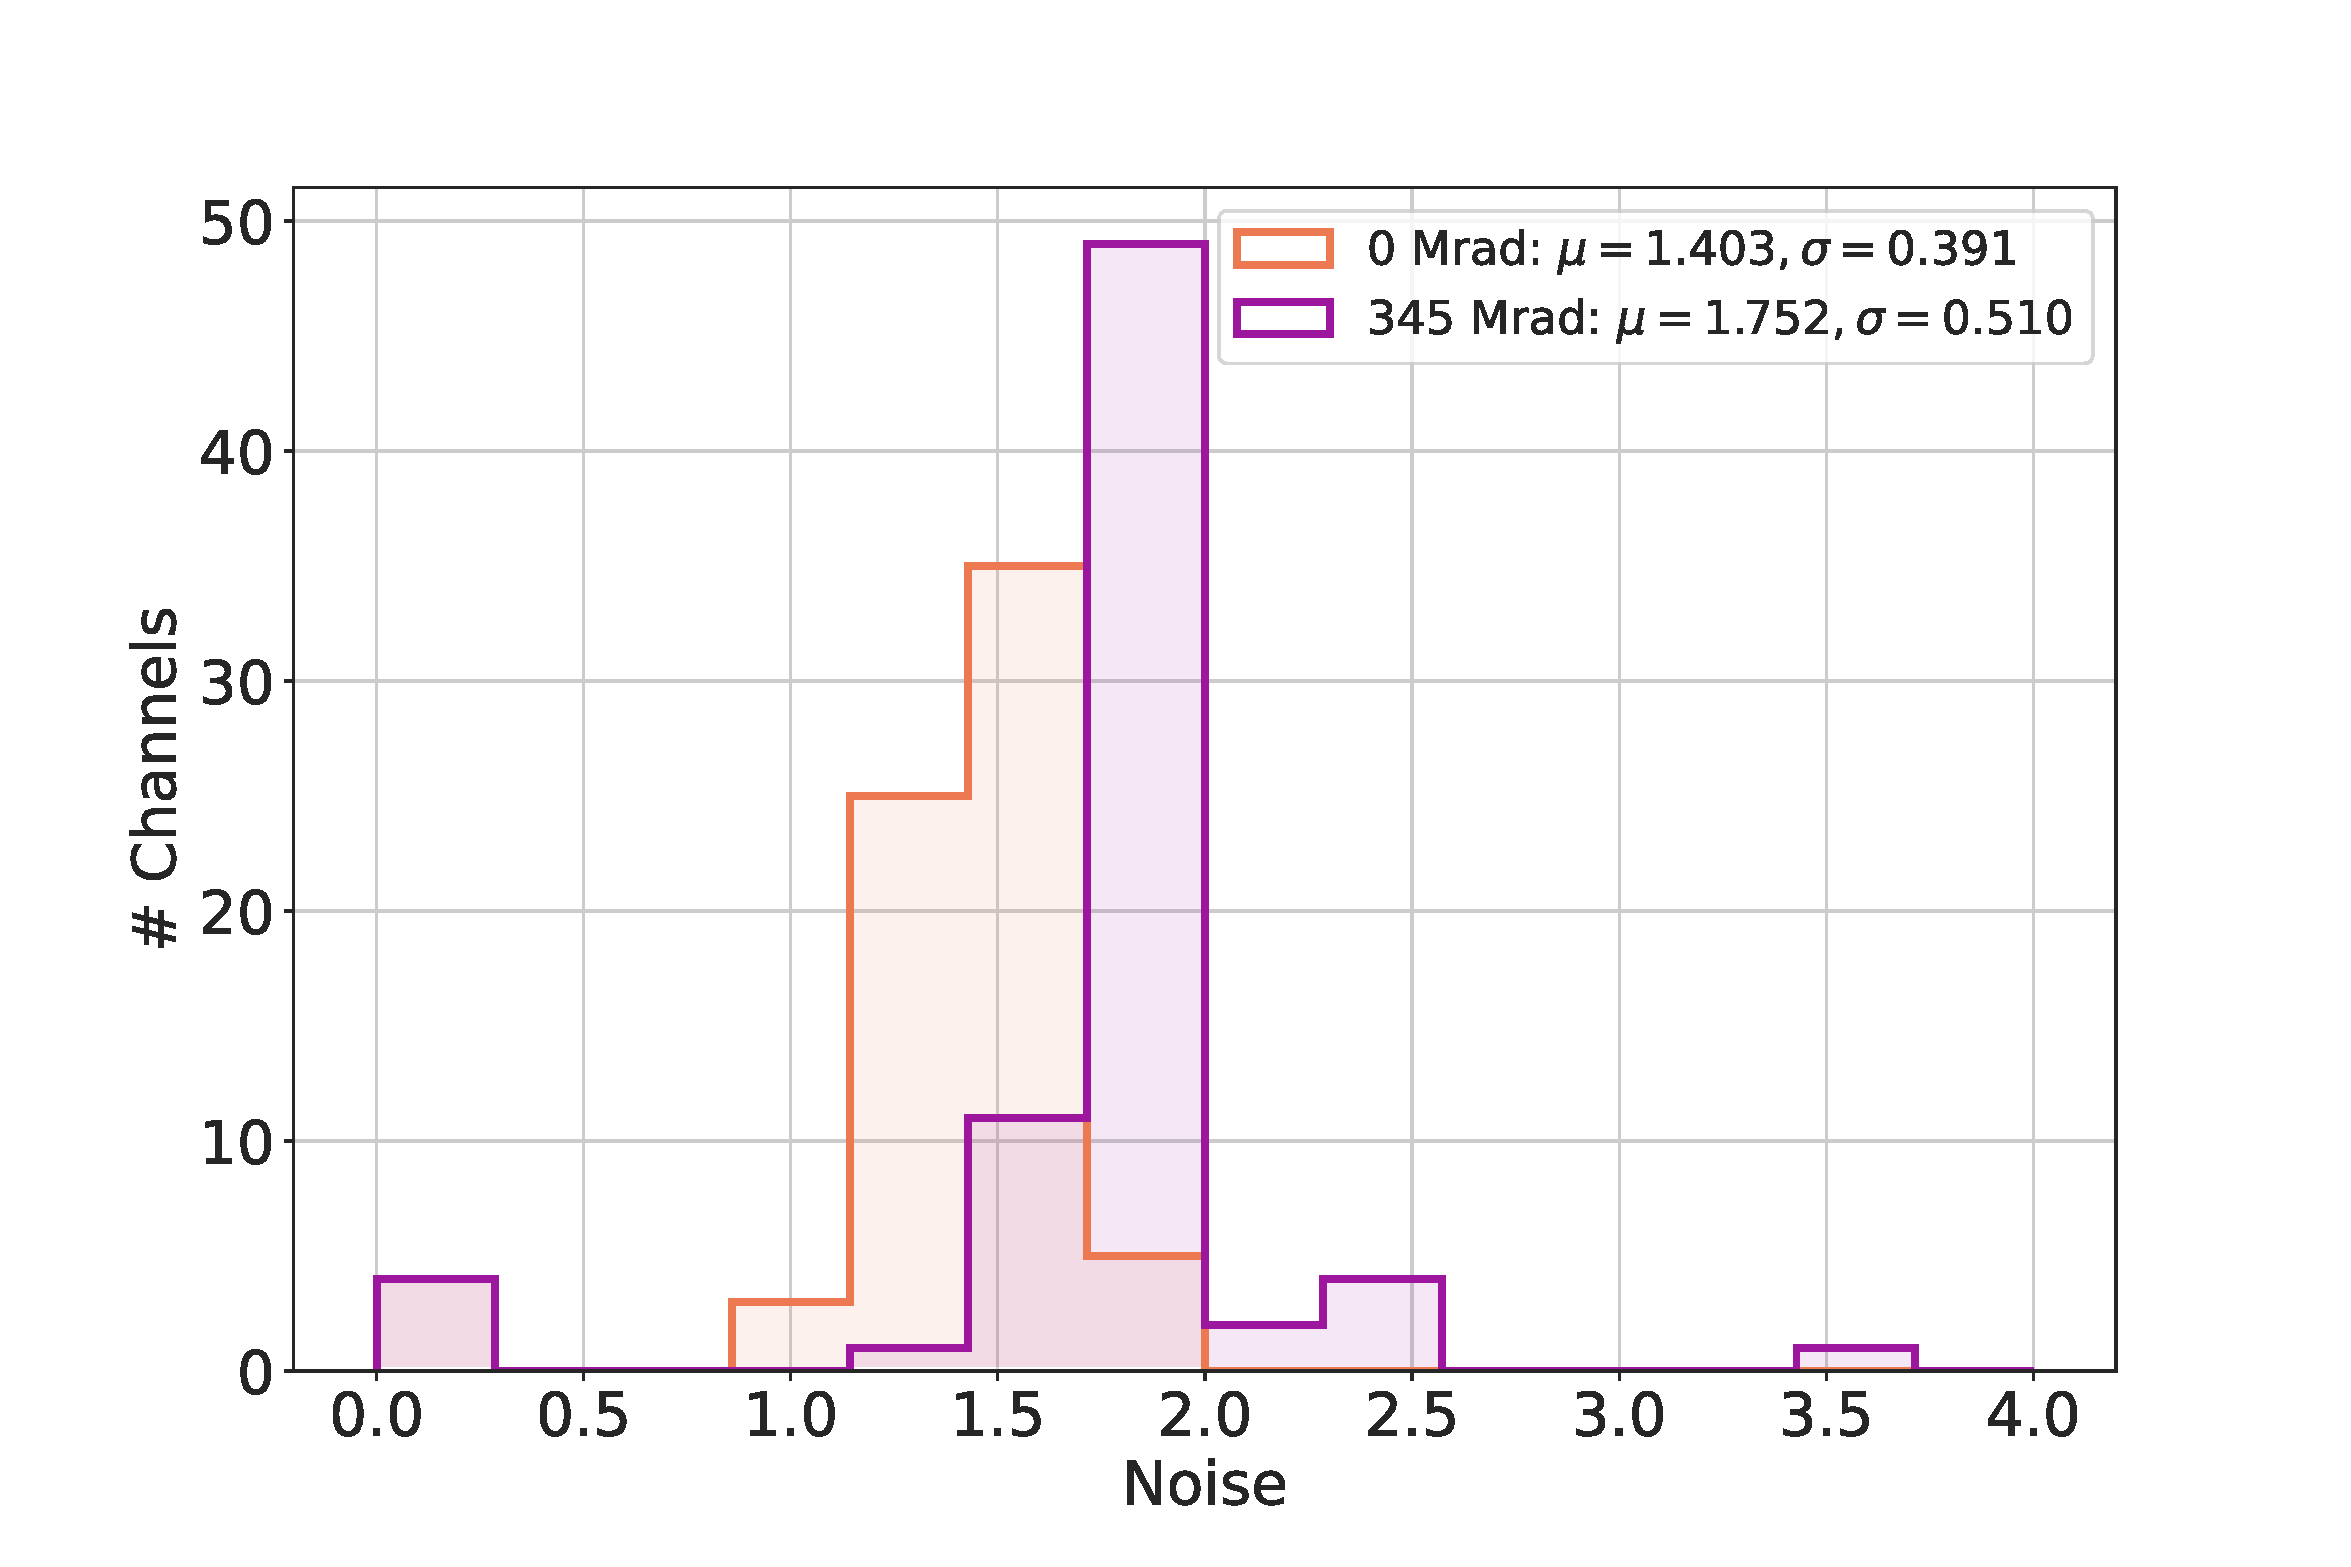
\includegraphics[width=0.65\linewidth]{Figures/HGCAL/TID_Noise.pdf}
    \caption{Distribution of the preamplifier noise for the 72 normal channels of the HGCROC3 at the beginning and at the end of the TID irradiation campaign. An average +$20\%$ increase in the noise is observed. The 4 zero-noise channels in the first bin are already present at the beginning of the irradiation and are due to imperfect chip manufacturing.}
    \label{fig:TID_Noise}
\end{figure}

\subsection{Effects on the power consumption}
\label{subsec:Power consumption}

The power consumption of the HGCROC3 device has been investigated during the exposure time, in terms of bias voltage and current in the analog and the digital components of the chip separately.

The bias voltage shows a stable behaviour, while the current exhibit a +$25\%$ (+$8\%$) peak in the analog (digital) part corresponding to a dose of $10\;\textrm{Mrad}$. This large variation is followed by a slow decrease during the radiation exposure, as illustrated in Figure~\ref{fig:TID_Power}.

\begin{figure}
    \centering
    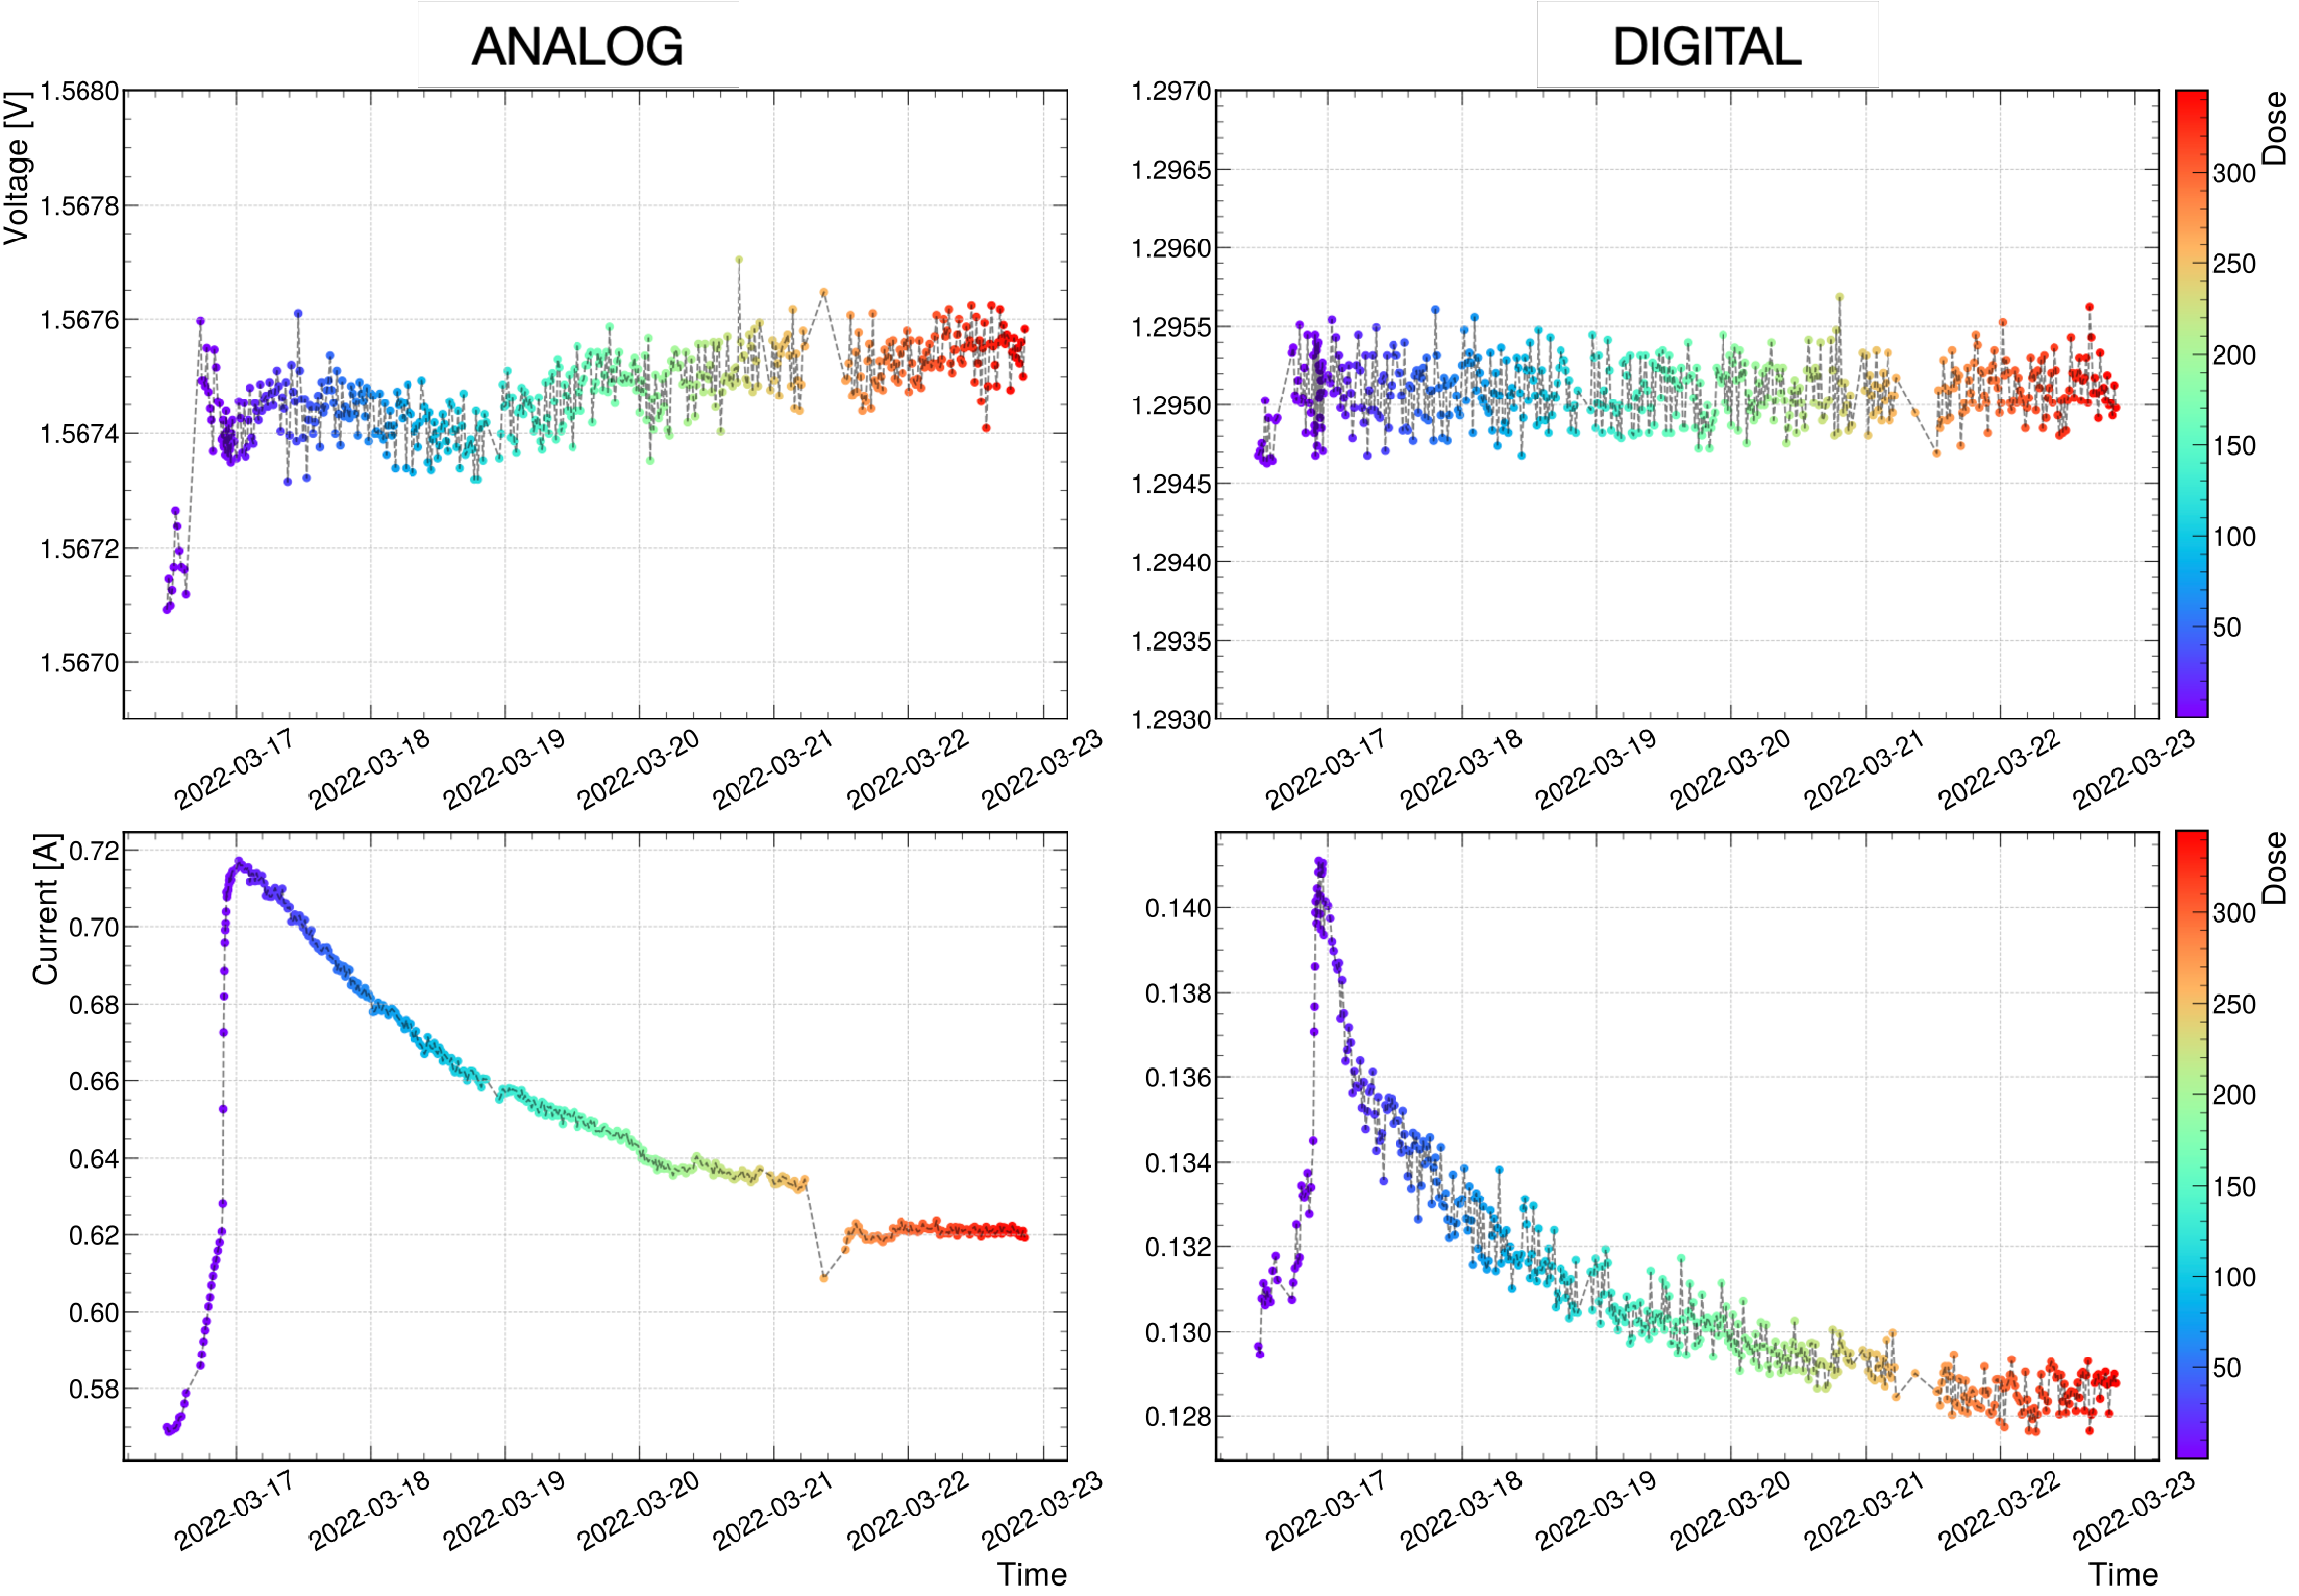
\includegraphics[width=0.99\linewidth]{Figures/HGCAL/TID_Power.pdf}
    \caption{Measurement of the analog and digital power consumption of the HGCROC3 during the radiation exposure as a function of the time and the injected dose.}
    \label{fig:TID_Power}
\end{figure}

\bigbreak

The process causing the current increase is well documented in the literature and it is related to the presence of leakage current in the transistors. 
As illustrated in Figure~\ref{fig:TID_Transistors}, when transistors are exposed to ionizing radiation, such as X-rays, the particles crossing the device can create electron-hole (e-h) pairs in the silicon substrates. Since the electrons have a high mobility, they are quickly removed, while holes are trapped in low-energy traps and the build up of charge creates a distribution of positive charge close to the interface of the gate oxide, resulting in a voltage threshold shift and a leakage current. 

Small size transistors, such as the ones employed in the digital compartment of the HGCROC3, are usually more affected by the leakage current; however, the effect is expected to decrease with lower dose rate, hence the digital power consumption peak in the HGCROC3 is estimated to be within the acceptable limits and does not constitute a major concern.

On the contrary, the effects of the leakage current on large size transistors, such as the ones employed in the analog part of the HGCROC3, are expected to be significantly reduced. For this reason, the unexpected analog current increase observed during the TID irradiation campaign arises suspicions about the circuit and deserves a closer investigation.

\bigbreak

Additional TID irradiation campaigns have been performed on various HGCROC3 prototypes in order to understand the source of the analog current increase. 
Table~\ref{tab:TID_Current} reports the results on three devices, irradiated under different conditions of dose rate and temperature.
The results confirm the presence of a current increase in all devices, both in the analog and in the digital part of the chip. The digital increase is stable and not affected by temperature nor dose rate in the investigated range. The analog increase does not show dependence on the dose rate, but the peak is reduced at lower temperature.
In order to identify the region of the circuit responsible for the current increase, the power consumption is measured under different settings, by consecutively switching off different parts of the ADC analog chain. The analog current increase is still present when the full ADC chain is not connected, pointing to a possible source of leakage current in the TDC chain.

\bigbreak

Further investigation has been conducted on irradiated devices in order to locate the source of the leakage current. With the help of a thermal camera it has been possible to highlight the regions of the chip where the current is higher than expected and the leakage source is confirmed to be coming from the TDC component.
The study and simulation of the TDC circuit has finally pointed to a floating input node left in high impedance when no conversion is happening.
% The input voltage should be fixed either to Vgnd=0 or Vdd=1 V, but the leakage current can shift the input value and when A=0.5 V there is current flowing in the circuit. 
This  condition does not affect the TDC operations but leads to high leakage current in the downstream NOR gate. Simulations of the circuit can reproduce a current that is compatible with the one observed during the irradiation campaigns.
A correction for this defect has been included the HGCROC3b design.

\begin{figure}
    \centering
    \subfloat[]{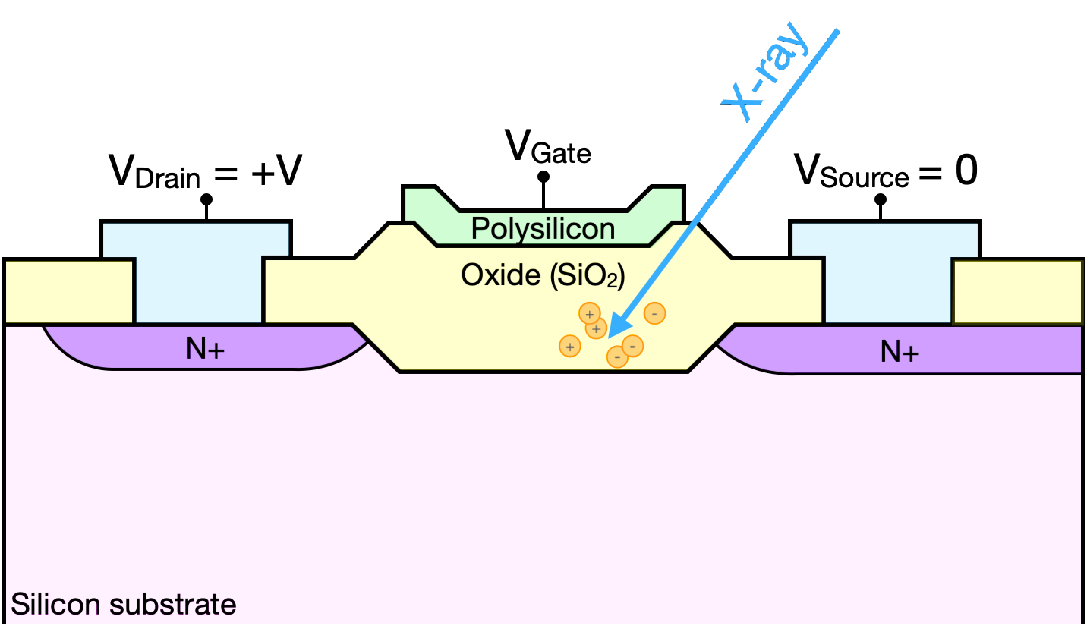
\includegraphics[width=0.3\linewidth]{Figures/HGCAL/TID_Transistors1.pdf}}
    \hspace{0.1cm}
    \subfloat[]{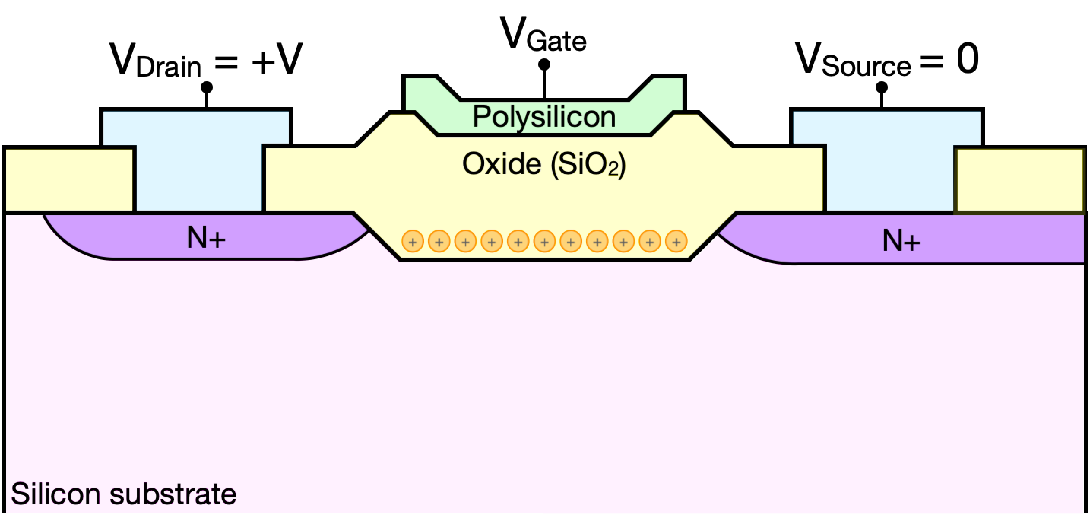
\includegraphics[width=0.3\linewidth]{Figures/HGCAL/TID_Transistors2.pdf}}
    \hspace{0.1cm}
    \subfloat[]{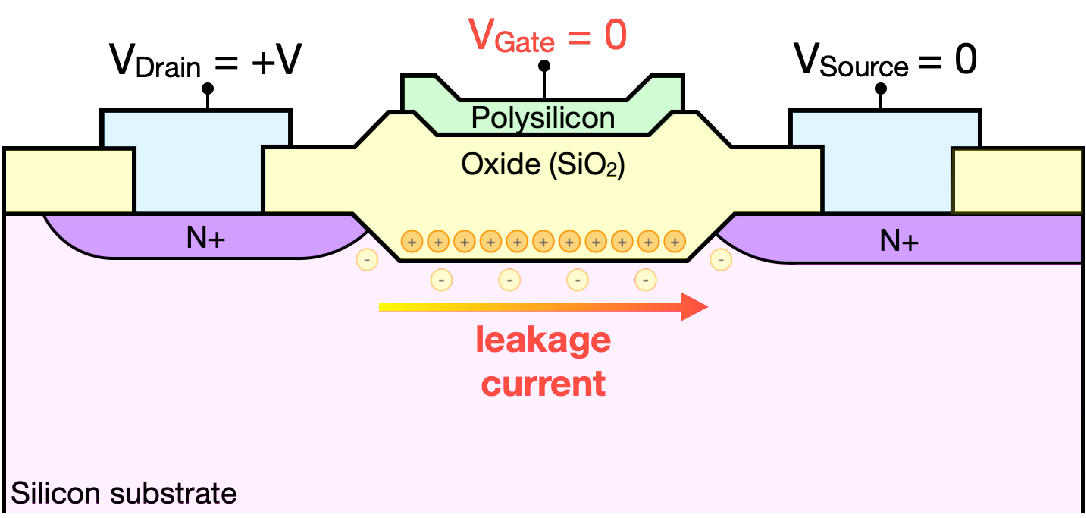
\includegraphics[width=0.3\linewidth]{Figures/HGCAL/TID_Transistors3.pdf}}
    \caption{Illustration of the TID damage in transistors due to hole trapping in the silicon oxide ($\textnormal{SiO}_2$). A ionising particle, like X-rays, crossing the device creates e-h pairs (a): electrons have a high mobility and are quickly removed, while holes are trapped in low-energy traps (b). The build up of charge creates a distribution of positive charge close to the interface of the gate oxide, leading to voltage threshold shifts or leakage current (c).}
    \label{fig:TID_Transistors}
\end{figure}

\begin{table}
    \centering
    \begin{tabular}{c|c|c|c|c}
        \hline
        \hline
        Chip Number & Dose Rate & Temperature & Analog Increase & Digital Increase \\
        \hline
        ROC 003 & 2.5 Mrad/h & $+20^{\circ}$C & 0.40 A & 0.015 A \\
        ROC 000 & 2.5 Mrad/h & $-10^{\circ}$C & 0.175 A & 0.015 A \\
        ROC 015 & 0.3 Mrad/h & $-10^{\circ}$C & 0.175 A & 0.015 A \\
        \hline
        \hline
    \end{tabular}
    \caption{Results from three TID campaigns performed on prototypes of HGCROC3 with different dose rate and temperature conditions for the investigation of the analog and digital current increase during the radiation exposure.}
    \label{tab:TID_Current}
\end{table}

\bigbreak

The TID irradiation campaign has proven to be fundamental in evaluating the radiation tolerance of the HGCROC3 up to $200\,\textrm{Mrad}$. The successful execution of this campaign under various conditions has provided crucial insights into the device resilience in radiation-prone environments. 
Moreover, it has highlighted the presence of a floating input node in the TDC circuit, an issue that could be rectified before finalising the HGCROC3b design and initiating large-scale production. 

%%%%%%%%%%%%%%%%%%%%%%%%%%%%%%%%%%%%%%%%%%%%%%%%%%%%%%%%%%%%%%%%%%%%%%%%%%%%%%%%%%%%%%%%%%%%
%%%%%%%%%%%%%%%%%%%%%%%%%%%%%%%%%%%%%%%%%%%%%%%%%%%%%%%%%%%%%%%%%%%%%%%%%%%%%%%%%%%%%%%%%%%%
%%%%%%%%%%%%%%%%%%%%%%%%%%%%%%%%%%%%%%%%%%%%%%%%%%%%%%%%%%%%%%%%%%%%%%%%%%%%%%%%%%%%%%%%%%%%
%%%%%%%%%%%%%%%%%%%%%%%%%%%%%%%%%%%%%%%%%%%%%%%%%%%%%%%%%%%%%%%%%%%%%%%%%%%%%%%%%%%%%%%%%%%%

\section{Single Event Effect campaigns}
\label{sec:Single Event Effect}

The Single Event Effect (SEE) irradiation test aims at evaluating the radiation damage induced by a single energetic particle on electronic devices. Differently from the TID irradiation test, the SEE induces very localised and non-cumulative effects causing potential malfunctioning inside the data-processing system with multiple consequences. Given the stochastic nature of the effect, it can occur at any moment since the beginning of the operation.

The SEE events could become an important issue for high-energy particle physics experiments, not much because a small fraction of the enormous data stream could be corrupted, but because some vital detector control functions could be lost due to memory upsets. It is thus important to preserve the device from this source of potential danger, by implementing tools to secure the static memory registers storing the logic configuration.

\bigbreak

A SEE is caused by a very high energy deposition in a small volume of the electronic device. The single ionizing particle crossing the silicon device creates a sudden and sharp charge release, generating electron-hole (e-h) pairs. In the silicon substrate, the charge is collected at one of the microcircuit nodes and produces a temporary current transient in the circuit. 

% Three possible consequences can occur:
% \begin{itemize}
%     \item [-] \textit{Single Event Upset} (SEU): a bit storing the logic information is flipped,
%     \item [-] \textit{Single Event Transient} (SET): a shift in the string of bits,
%     \item [-] \textit{Single Event Latch-up} (SEL): a short circuit in part of the device causing permanent damage.
% \end{itemize}

% \begin{itemize}
%     \item [-] Single Event Upset (SEU): digital error, or bit flip.
%     \item [-] Single Event Transient (SET): analog error,  or bit shift.
%     \item [-] Single Event Latch up (SEL): permanent damage of the device.
% \end{itemize}

As a consequence of a high energy deposition in the device, three possible effects can occur:
\begin{itemize}
    \item The \textit{Single Event Upset} (SEU) is a non-destructive phenomenon inducing a flip in the bits that store the logic information. The cause lies in the digital part of the electronic device, based on transistor technology, where the one-bit memory element is designed to have two possible stable states: 0 or 1. A SEU event appears as an error in the information stored either inside the dynamic or the static memory register, i.e. a bit flip from 0 to 1 or the opposite.
    \item The \textit{Single Event Transient} (SET) happens when the charge collection creates a spurious current signal changing one of the clock frequencies of the device. The frequency is usually provided to the chip by an analog synthesizer inside the PLL module: if a glitch affects the output signal of this module, all the activities in the chip can suffer from a temporary loss of synchronization, resulting in an undesirable circuit response that can vary depending on the circuit topology and the amount of charge collected.
    \item The \textit{Single Event Latch-up} (SEL) is a permanent destructive event where the current induced by the incident particle is so high that creates a short circuit in a part of the device.
\end{itemize}

The magnitude of these effects and their occurrence depends on the circuit topology and on the characteristics of each particle interaction, including the charge collection efficiency and the time constants of the perturbation effect. 

\subsection{Ionisation form different particles}
\label{subsec:SEE with Heavy Ions}

\begin{figure}
    \centering
    \subfloat[]{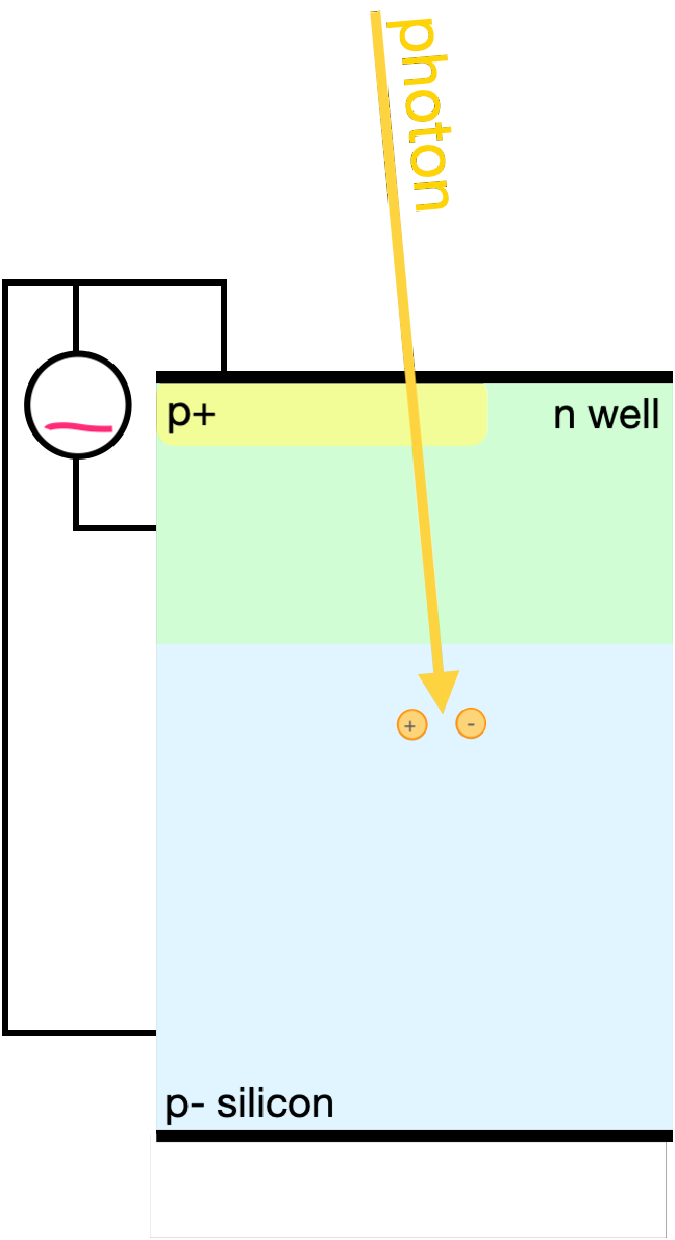
\includegraphics[width=0.22\textwidth]{Figures/HGCAL/SEE_ParticleInteraction1.pdf}}
    \hspace{0.1cm}
    \subfloat[]{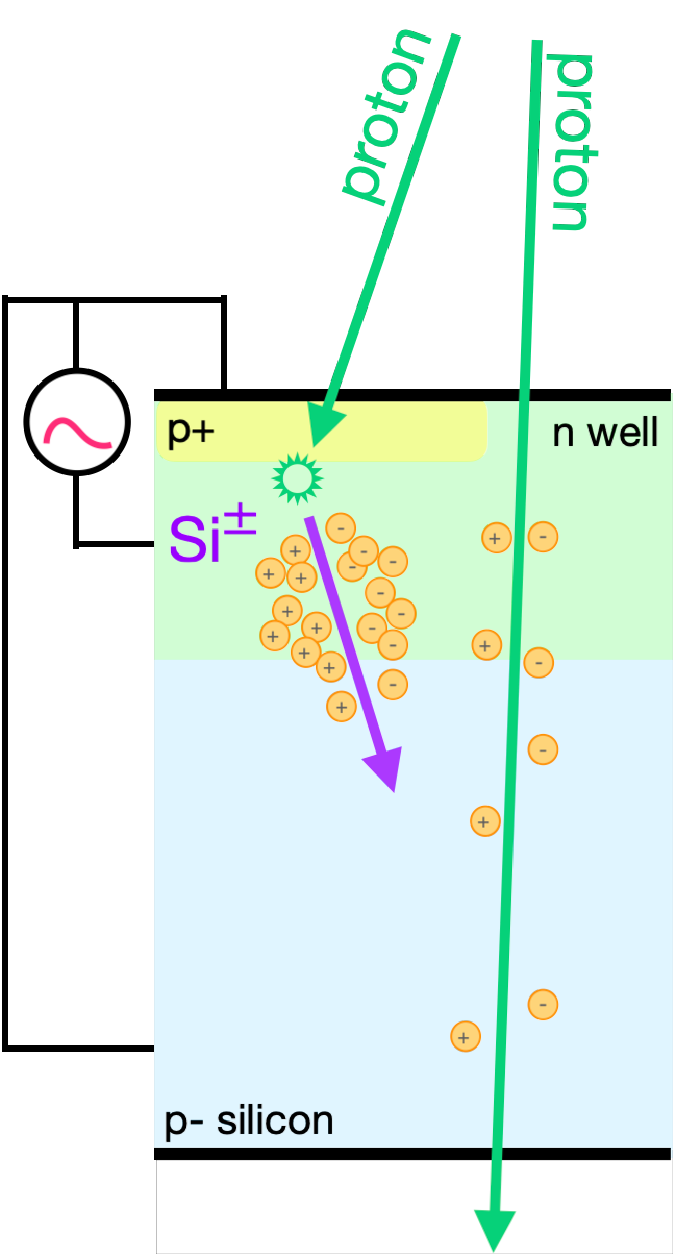
\includegraphics[width=0.22\textwidth]{Figures/HGCAL/SEE_ParticleInteraction2.pdf}}
    \hspace{0.1cm}
    \subfloat[]{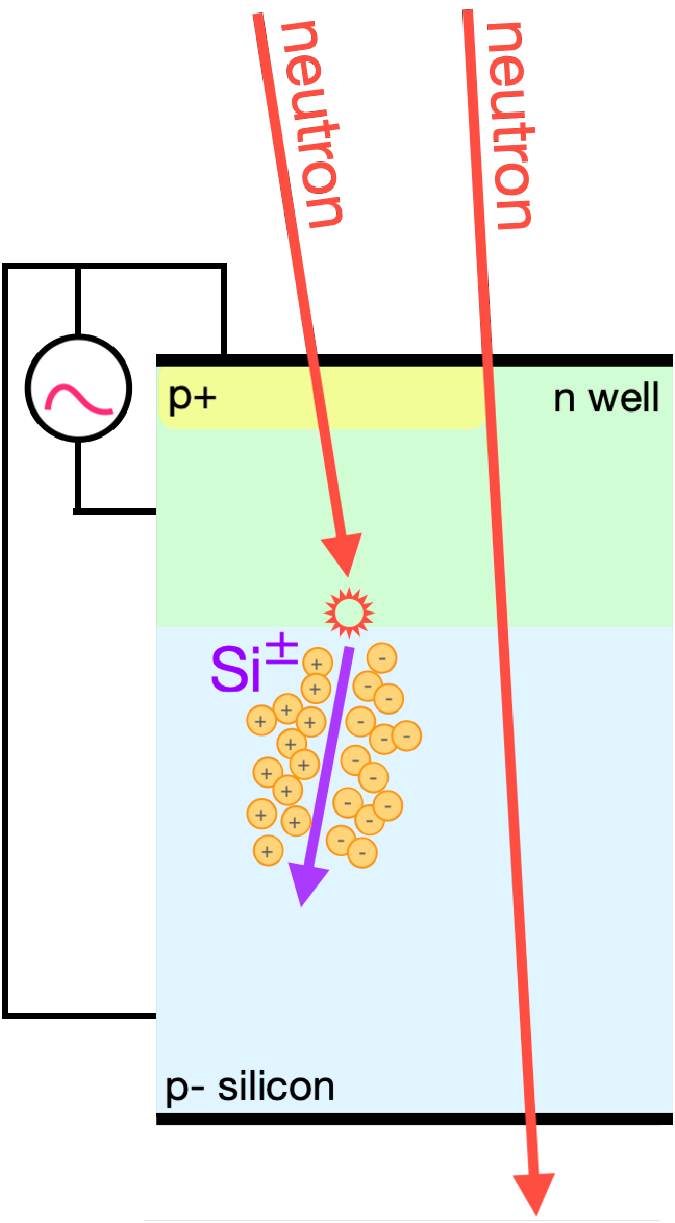
\includegraphics[width=0.22\textwidth]{Figures/HGCAL/SEE_ParticleInteraction3.pdf}}
    \hspace{0.1cm}
    \subfloat[]{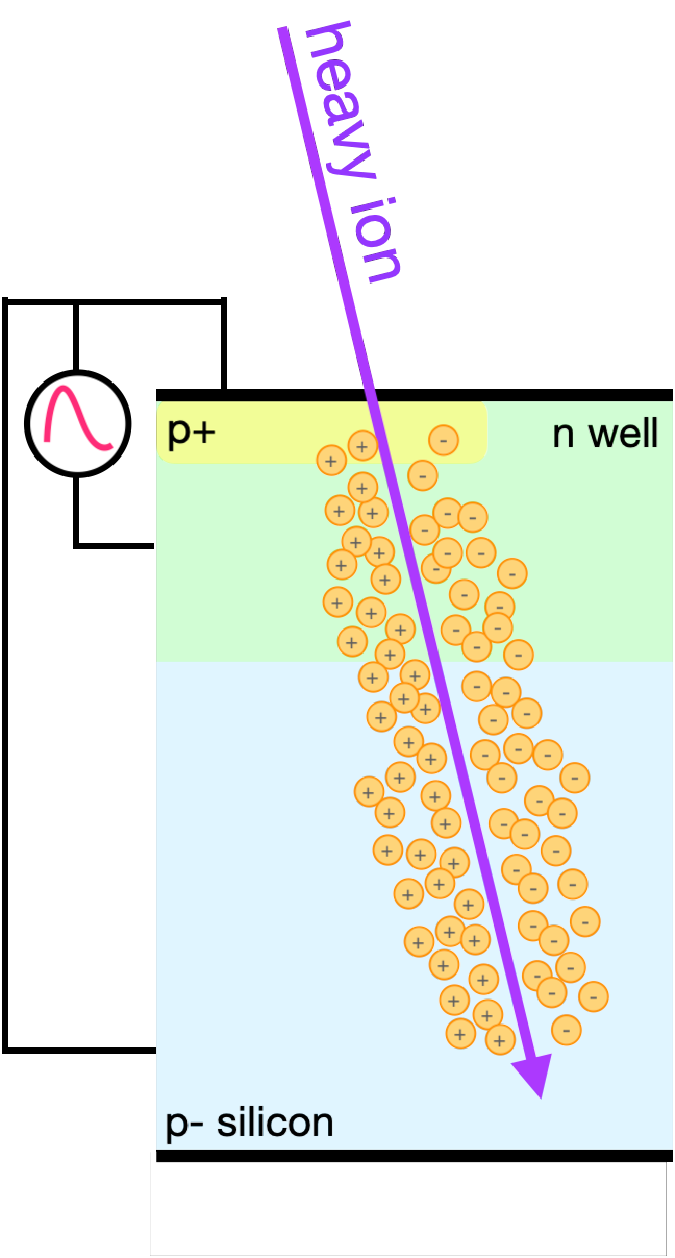
\includegraphics[width=0.22\textwidth]{Figures/HGCAL/SEE_ParticleInteraction4.pdf}}
    \caption{Schematic view of the ionisation induced by different particles in the silicon substrate. Photons (a) produce a small density of e-h pairs, not enough to provoke an instantaneous current variation in the circuit. Protons (b) and neutrons (c) release small (no for neutrons) charge through direct ionisation, while a high density of e-h pairs is produced from the nuclear interaction with the Silicon nuclei. Heavy ions (d) induce extremely large production of e-h pairs, with a notable impact on the device.}
    \label{fig:SEE_ParticleInteraction}
\end{figure}

In the HL-LHC radiation environment, different particles can hit the HGCAL read-out system, with different effects depending on the interaction process and the density of e-h pairs produced. 

\bigbreak

The main energy loss mechanisms for charged particles inside matter are \textit{ionization} and \textit{Bremsstrahlung}, where the former is predominant for high mass particles. 
The energy loss is described through the Stopping Power or Linear Energy Transfer (LET), which is defined as the amount of incident particle energy deposited per unit track length in the material of interest.
The energy loss of a minimum ionizing particle (e.g. a proton of about 2~GeV) in silicon is about 3.9~MeV/cm. This energy loss increases rapidly with decreasing energy of the particle, following the Bethe-Bloch formula, up to reaching a maximum of around 100~keV of kinetic energy.

The ionization directly induced by protons and other charged light hadrons is not dense enough to provoke current variation in the circuit. 
However, light hadrons can produce a nuclear interaction in the silicon substrate, kicking a Silicon nucleus out of the lattice structure: the charged nuclear recoil is itself an ionizing particle with low energy (usually $<10$~MeV) and limited penetration range ($<10$~$\mu$m), but has significantly high LET (about 30~GeV/cm) and creates a large amount of current inside the circuit.
The probability of a nuclear interaction caused by protons and neutrons is generally low, around $~10^{-5}$, but given the high flux of particles, the effect is non-negligible and provides the main source of SEE errors at the LHC.

In order to more effectively simulate the effect of the Silicon nuclear recoil, the SEE irradiation tests are often performed using heavy ions. 
A heavy ion is characterized by high LET, increasing with the ion mass, and a large penetration range, so that it can produce a large amount of charge in the silicon substrate, much bigger than the nuclear interaction caused by protons and neutrons.
As a consequence, heavy ions provide a good method to stress test the device in SEE irradiation campaigns and are commonly used as an alternative to protons.

\bigbreak

A schematic view of various particles interacting with the silicon substrate of the transistor is provided in Figure~\ref{fig:SEE_ParticleInteraction}.
Photons, such as X-rays and $\gamma$-rays, produce a small density of e-h pairs, which is not enough to provoke an instantaneous current variation in the circuit. 
Small (for protons) or no (for neutrons) charge is released through direct ionisation, while a high density of e-h pairs is produced from the nuclear interaction with the Silicon nuclei. Heavy ions have extremely high LET and induce a large production of e-h pairs, with a notable impact on the device.

% https://indico.cern.ch/event/635099/contributions/2570672/attachments/1456364/2249943/Single_Event_Effecs_Radiation_Course_May_2017_SEE_CBP.pdf

\subsection{Single Event Effect with Heavy Ions}
\label{subsec:SEE with Heavy Ions}

The first SEE campaign has been performed using a beam of low-energy heavy ions at the UCL cyclotron (Louvain, BE).
The facility provides several types of heavy ions with different values of mass-to-charge ratio (M/Q) and LET.
Since the heavy ions have to penetrate a Silicon layer of approximately 70~$\mu$m before reaching the area of the device interested by SEE, a correction is applied to compute the effective LET of each ion after crossing 70~$\mu$m of Silicon. The corresponding value is reported in Table~\ref{tab:SEE_Ions}.

\begin{figure}[t]
    \centering
    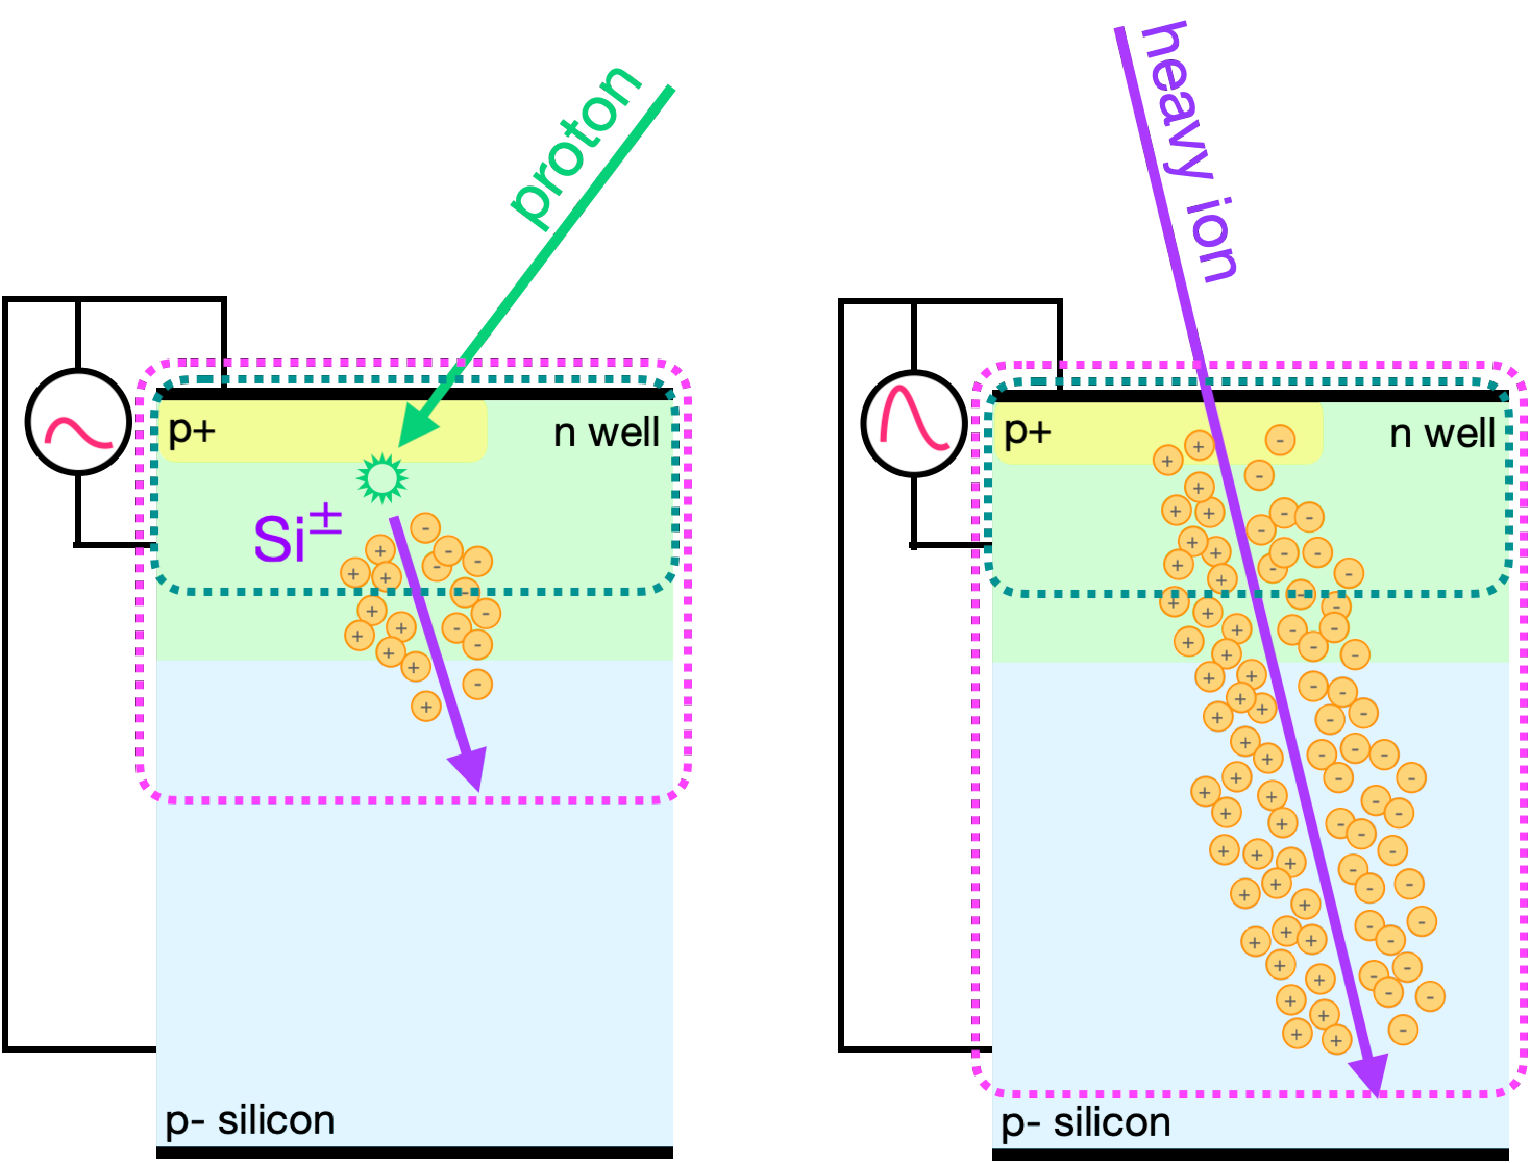
\includegraphics[width=0.45\linewidth]{Figures/HGCAL/SEE_SV.pdf}
    \caption{Difference between light hadrons (protons and neutrons) and heavy ions irradiation: the digital SV (dashed blue line) is typically smaller than the analog SV (dashed pink line).}
    \label{fig:sensitivevolume}
\end{figure}

\begin{table}
    \centering
    \begin{tabular}{c | c | c | c | c}
        \hline
        \hline
        \multirow{2}{*}{Ion} & \multirow{2}{*}{M/Q} & Range & LET & Effective LET \\
        &  & [$\mu$m] & [$\textrm{MeV}/\textrm{mg}/\textrm{cm}^2$] & [$\textrm{MeV}/\textrm{mg}/\textrm{cm}^2$] \\
        \hline
        Ne & 3.14 & 202.0 & 3.3 & 4 \\
        Al & 3.37 & 131.2 & 5.7 & 8.26 \\
        Ar & 3.33 & 120.5 & 9.9 & 14.76 \\
        Cr & 3.31 & 107.6 & 16.0 & 25.2 \\
        Ni & 3.22 & 100.5 & 20.4 & 31.1 \\
        Kr & 3.35 & 94.2 & 32.4 & 38.5 \\
        Xe & 3.54 & 73.1 & 62.5 & $<$10 \\
        \hline
        \hline
    \end{tabular}
    \caption{List of the available heavy ions at the UCL cyclotron. Each ion is characterised by a different mass-to-charge ratio (M/Q), penetration range in Silicon material, and Linear Energy Transfer (LET).}
    \label{tab:SEE_Ions}
\end{table}

\bigbreak

Since the HL-LHC radiation environment will be dominated by light hadrons, like protons and neutrons, some fundamental differences in the particle interactions have to be considered when characterizing a device with heavy ions.
The SEE occurrence depends on the \textit{Sensitive Volume} (SV) of the device, which is defined as the region where the charge collection can contribute to a possible alteration of the circuit:
\begin{itemize}
    \item [-] for a SEU on the digital part, a very fast current signal is required: the digital SV is usually small and there is no radical difference between heavy ions and protons;
    \item [-] for a SET on the analog part, all the signals can have a contribution: the analog SV significantly depends on the particle type, making the heavy-ion irradiation an unreliable estimate in terms of SETs.
\end{itemize}

Figure~\ref{fig:sensitivevolume} shows the difference between the analog and digital SV for protons with respect to heavy ions.
The heavy ion irradiation campaign can provide an effective alternative to protons for the estimation of the SEU on the digital component of the device, but cannot be considered a reliable estimate for the SET on the analog part.
The heavy ion irradiation test also furnish a very important stress test for SEL: as proposed in \cite{federico}, the absence of latch-ups for high LET values (around 40~MeV/mg/$\textrm{cm}^2$) will guarantee the robustness of the device against latch-ups in any accelerator environment.

\bigbreak

During the SEE campaign, a prototype of the HGCROC3 is closed in a vacuum chamber at a stable temperature of 7.2~$^{\circ}$C and irradiated with beams of various heavy ions, with different values of mass and LET, at a fixed flux of $10^4$~$\textrm{s}^{-1}\,\textrm{cm}^{-2}$. 
The digital components of the HGCROC3 have been tested by performing two sets of measurements: the I2C and the DAQ test.

\subsubsection{I2C test}

\begin{figure}
    \centering
    \subfloat[]{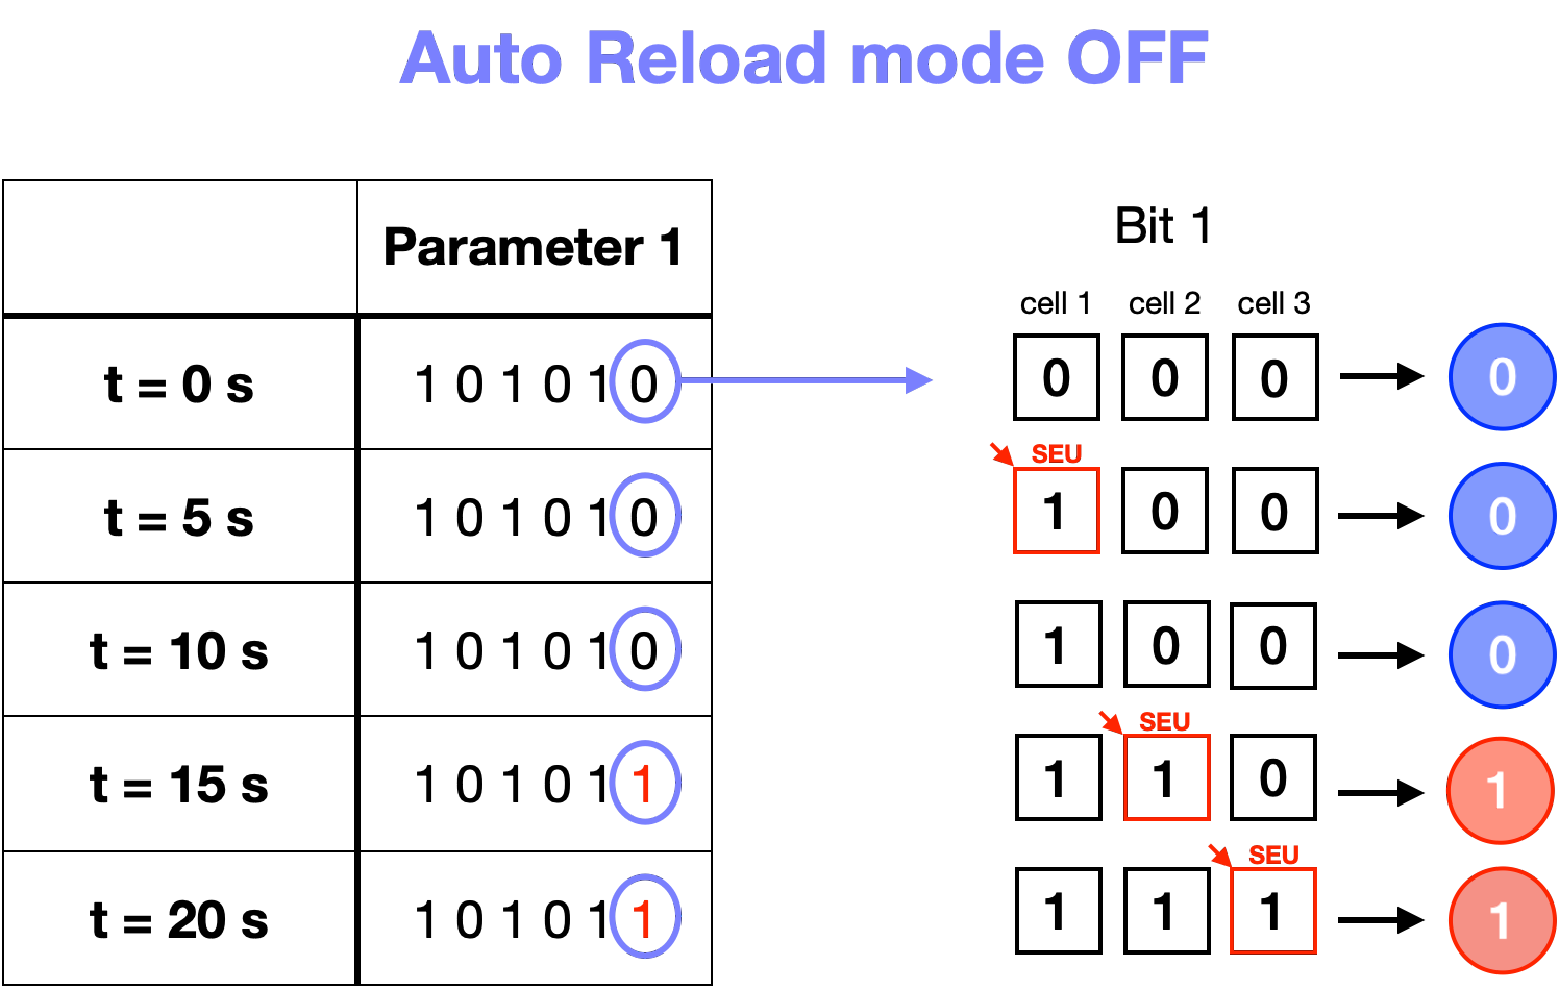
\includegraphics[width=0.45\linewidth]{Figures/HGCAL/SEE_AutoreloadOFF.pdf}}
    \hspace{1.cm}
    \subfloat[]{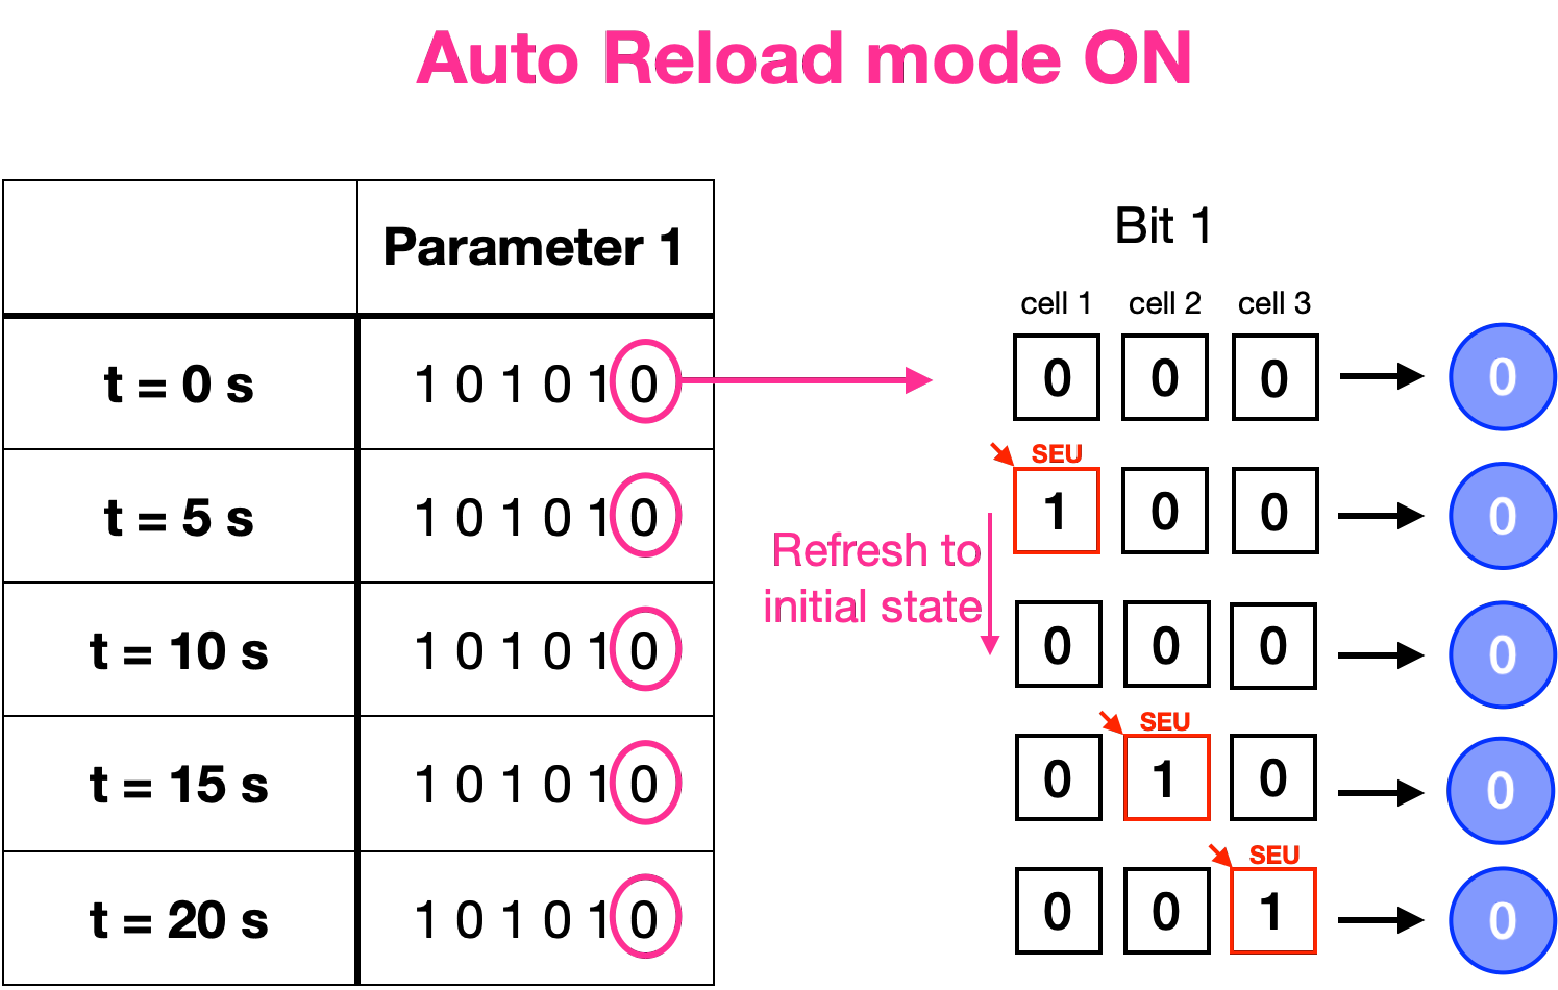
\includegraphics[width=0.45\linewidth]{Figures/HGCAL/SEE_AutoreloadON.pdf}}
    \caption{Representation of the \textit{Triplication} logic with \textit{AutoReload} mode enabled (a) or disabled (b). The values of the I2C bits are stored in three different cells: if a SEU event changes the value of one cell, the majority vote prevents the bit flip. When the \textit{AutoReload} mode is enabled, as soon as a change in the values is detected, the three cells are refreshed according to the majority vote.}
    \label{fig:Autoreload}
\end{figure}

The I2C of the HGCROC3 holds 2,573 configuration parameters, encoded in 8,956 bits, storing the device configuration and operation settings. 
Before starting the irradiation test, all the parameters are correctly set to given values, and during irradiation the I2C registers are read to check for possible bit flips.

In order to protect the I2C registers against possible SEUs, the I2C bits use the \textit{Triplication} logic: the value of each bit is stored into three different cells, such that if a SEU event changes the value of one cell, the logic of the majority still keeps the bit value to the original one, as represented in Figure~\ref{fig:Autoreload}a. However, if two or more SEU events impact the same bit, the value is corrupted and the triplication logic on its own does not suffice for long irradiation exposure. 
An additional protection against bit flips is provided by the \textit{AutoReload} mode, which allows for a continuous check of the cell values such that, if inconsistency between the values of the triplicated cells is found, the I2C sends a command to refresh all the cells according to the majority vote, as represented in Figure~\ref{fig:Autoreload}b.

During irradiation, all the I2C bits are monitored and the resulting numbers of errors are summarized in Table \ref{tab:I2C}: while multiple bit flips are observed when the \textit{AutoReload} mode is disabled, no bit flip is observed when the \textit{AutoReload} mode is enabled. The I2C test results show the successful capability of the \textit{AutoReload} mode in preventing SEU on the HGCROC3 I2C registers.

\begin{table}
    \centering
    \begin{tabular}{c | c c | c c}
        \hline
        \hline
        % [$\textrm{MeV}/\textrm{mg}/\textrm{cm}^2$]  [$\textrm{part}/\textrm{s}/\textrm{cm}^2$]
        & \multicolumn{2}{c |}{AutoReload OFF} & \multicolumn{2}{c}{AutoReload ON} \\
        Ion & Time [s] & Bit flips & Time [s] & Bit flips \\
        \hline
        Ne & 490 & 55 & 1515 & 0 \\
        Al & 490 & 213 & 1291 & 0 \\
        Ar & 699 & 316 & 1184 & 0 \\
        Cr & 687 & 559 & 879 & 0 \\
        Ni & 678 & 662 & 1289 & 0 \\
        Kr & 507 & 502 & 661 & 0 \\
        Xe & 641 & 130 & 127 & 0 \\
        \hline
        \hline
    \end{tabular}
    \caption{Results of the I2C test when the \textit{AutoReload} is disabled (OFF) or enabled (ON). The irradiation is performed with various types of heavy ions, with different LET values and acquisition times.}
    \label{tab:I2C}
\end{table}

\subsubsection{DAQ test}

The DAQ test aims to check for possible SEU errors on the Data and Trigger paths of the HGCROC3 under irradiation. 
A schematic view of the Data and Trigger paths can be found in Figure~\ref{fig:TriggerDataPath}.
The Trigger path transmits the trigger information to the back-end electronics: the energy recorded in different cells is summed and compressed to 7-bit information, and then concatenated in a 32-bit word packet preceded by a fixed pattern header.
The Data path contains the digitised charge and time information coming from the channels. The word packet is composed by a header, followed by the information coming from the common mode (CM), normal, and calibration (Calib) channels. In addition, a Cyclic Redundancy Check (CRC) flag is stored to check the integrity of the transmission, and a final idle word maintains synchronization between the transmitter and receiver.
Inside the Data path header, the bunch crossing, event and orbit counters are stored. 

The logic inside the Data and Trigger paths is not triplicated as, unlike the I2C static registers, the data processing is dynamic and constantly flowing from the chip to the downstream electronics. However, data is processed with the \textit{Hamming encoding}, a method that stores redundant bits in the word packet to allow for the identification and correction of single-bit errors and for the detection of double-bit errors, an algorithm known as Single Error Correction - Double Error Detection (SEC-DED). The only triplicated information in the Data path is the bunch crossing, event, and orbit counter, since SEU errors on this information could become critical for the system operations. 

\bigbreak

During irradiation, the data processing is tested against SEU both for the triplicated and for the Hamming encoded information.
Since the potential bit flips could get lost among the random noise fluctuations of the data in a standard acquisition, a fixed data pattern is transmitted to all channels and compared to the output pattern.
The DAQ test is performed using multiple heavy ions with different LET and the results in terms of error numbers are reported in Table~\ref{tab:DAQ}. No error is detected in the counters, proving the successful protection of the triplication logic.
Only a few SEU events are observed on the non-triplicated trigger sums and in the CRC; the channel information is not significantly affected by SEU either, and in all cases the data corruption is detected by the Hamming encoding. 

By measuring the error rate under heavy ions irradiation with different values of LET, it would be possible to extrapolate the expected error rate in a proton radiation environment~\cite{federico}; in this case, due to the poor statistics, the heavy ion irradiation campaign is not able to provide a reliable estimate for the SEU error rate in the HL-LHC radiation environment.
However, the absence of glitches and latch-ups during the irradiation with Krypton, providing a LET of 38.5~MeV/mg/$\textnormal{cm}^2$, validates the protection of the HGCROC3 against SEL.

\begin{figure}
    \centering
    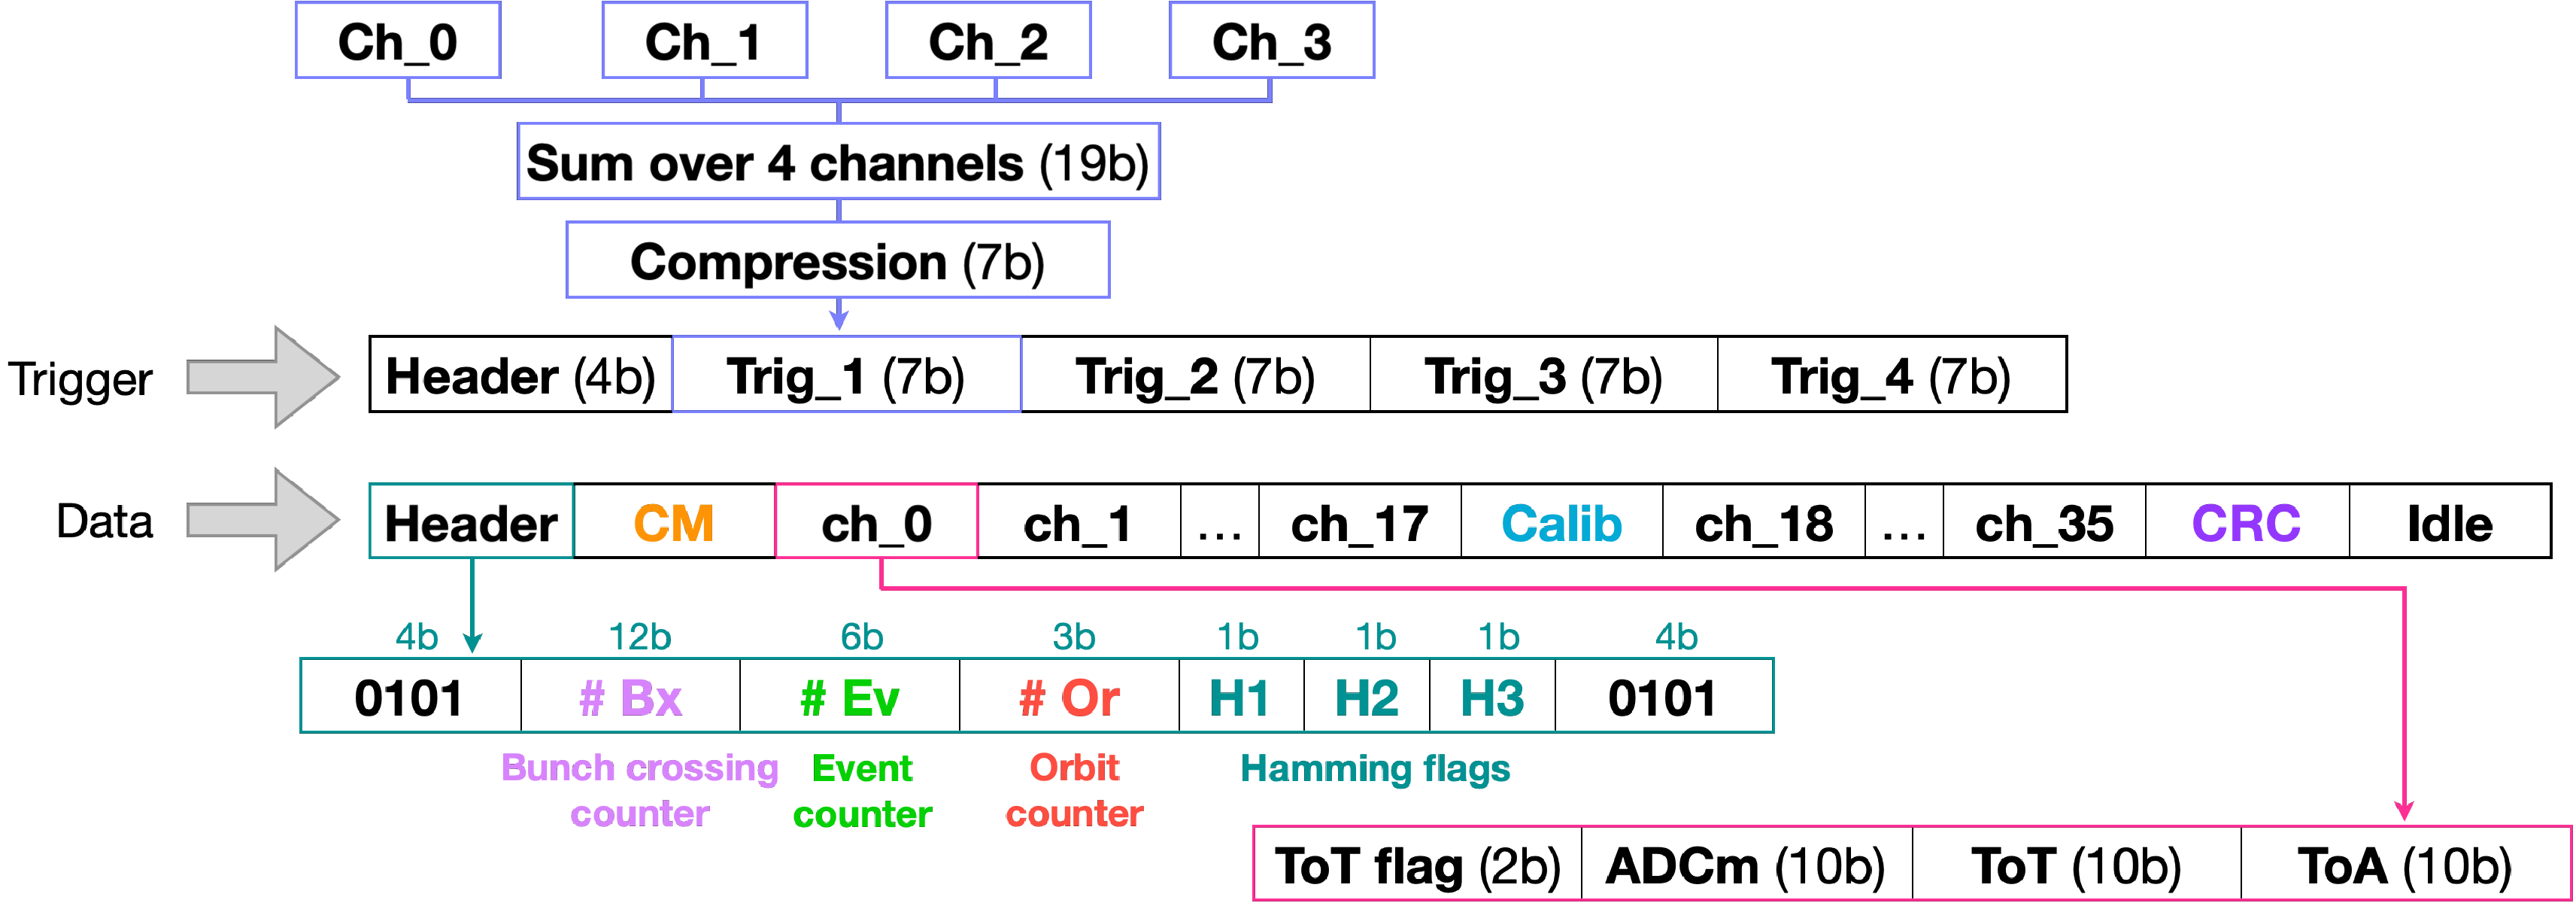
\includegraphics[width=0.95\linewidth]{Figures/HGCAL/TriggerDataPath.pdf}
    \caption{Scheme of the Trigger and Data paths of the HGCROC3. In the Trigger path, the energy sum of different channels is computed, the data is compressed and concatenated before being transmitted to the back-end electronics for the L1T decision. The Data path stores the information from the common mode (CM), normal, and calibration (Calib) channels; in the header, the counters for bunch crossing, event, and orbit are stored with triplicated logic.}
    \label{fig:TriggerDataPath}
\end{figure}

\bigbreak

During the DAQ test, several SET errors are observed on the analog part of the HGCROC3. The SET is due to particles releasing a large amount of charge in the PLL circuit, which provides the operation frequencies to the entire device: the sudden charge deposit can produce a change in the PLL output and variation in the frequency, causing link misalignments.
Two different types of SET errors have been identified:
\begin{itemize}
    \item [-] Short SET: the data transmission fails for just one bit and the rest of the data flow is correct; the CRC contains a corruption flag establishing an error in the data transmission.
    \item [-] Long SET: the transmission is in error for longer time, leading to a constant shift in the string of bits; the whole word packet is permanently shifted and the header pattern cannot be recognised by the downstream electronics. A link reset is required to recover the correct operation mode and restore the data flow.
\end{itemize}

Table~\ref{tab:DAQ} provides a summary of the number of SET events observed under irradiation with different types of heavy ions. 
When comparing the SEU and SET error rates, it is important to recall that the PLL is part of the analog component of the HGCROC3 and that the heavy ion irradiation provides too severe estimates for the SET rate with respect to the light hadron irradiation environment of the HL-LHC.

On the one hand, the presence of Short SET does not raise particular concern for the HGCROC3 operation, as the impact on the data processing and transmission is relatively low; on the other hand, the potential Long SET occurrence, even if at lower rate, would have a drastic impact on the device operation, not only because of the communication with the downstream electronics but also because of the potential corruption of a large quantity of trigger data from extended areas of the detector that could alter the data taking.

The heavy ion irradiation campaigns provide a serious red flag for the HGCROC3 vulnerability to SET, suggesting that a dedicated proton irradiation campaign is necessary to verify the potential presence of Long SET in the HL-LHC radiation environment and provide a more accurate estimate for the SEU and the SET rates. 

\begin{table}
    \centering
    \begin{tabular}{c | c | c c c c | c c}
        \hline
        \hline
        & & \multicolumn{4}{c |}{SEU} & \multicolumn{2}{c}{SET} \\
        Ion & Time [s] & Counters & Trigger & CRC & RAM & Long & Short \\
        \hline
        Ne & 1512 & - & - & - & - & - & - \\
        Al & 932 & - & - & 1 & - & - & - \\
        Ar & 934 & - & 1 & 1 & - & 1 & - \\
        Cr & 873 & - & - & - & 1 & 3 & 1 \\
        Ni & 911 & - & - & - & 2 & 8 & 2 \\
        Kr & 457 & - & - & - & - & 5 & 13 \\
        Xe & 128 & - & - & - & - & 1 & 8 \\
        \hline
        \hline
    \end{tabular}
    \caption{Results of the DAQ test in terms of SEU and SET events. The irradiation is performed with various types of heavy ions, with different LET values and acquisition times.}
    \label{tab:DAQ}
\end{table}

\subsection{Single Event Effect with Protons}
\label{subsec:SEE with Protons}

The second SEE campaign has been performed using a 64~MeV proton beam at the Arronax cyclotron (Nantes, FR).
Since the HGCAL radiation environment will be dominated by light hadrons, the proton irradiation gives a more realistic description of the expected HL-LHC environment with respect to heavy ions: as described in \cite{federico}, a proton energy of more than 60~MeV is sufficient to simulate all the possible radiation damage of the full proton energy range at the HL-LHC. Moreover, with the provided flux of $10^{10}\,\textrm{s}^{-1}\,\textrm{cm}^{-2}$, four orders of magnitude higher than the average expected HGCAL flux, it is possible to collect enough statistics in a relatively short amount of irradiation time.

\bigbreak

The proton irradiation set-up is more complex with respect to heavy ions and is represented in Figure~\ref{fig:SEE_Proton_Setup}. The proton beam is created in the centre of the Arronax facility, where the cyclotron is located, and then extracted through a beam pipe directed to a dedicated experimental cavern. 
Since protons have a higher potential for neutron production when interacting with materials, the experimental protocol necessitates extensive shielding and safety measures to protect both the equipment and the personnel from secondary radiation. 

The mezzanine board hosting the HGCROC3 prototype is aligned with the proton beam, and a collimator is used for a more precise beam localisation. 
The powering modules and the hexacontroler for the data acquisition are located at a safe distance from the beam and protected through plastic-lead shielding.
During irradiation, access to the cavern is not permitted and the data acquisition is entirely performed from an adjacent control room. Even after the end of the irradiation campaign, access to the cavern is restricted and the irradiated material needs to wait for radioactive isotopes to decay to safe levels before being returned.

\bigbreak

The main target of the proton campaign is to test the HGCROC3 against SEU and SET effects, collecting higher statistics with respect to the previous heavy ion campaign. 
The digital components of the HGCROC3 are tested by performing the same DAQ test described in the Section~\ref{subsec:SEE with Heavy Ions}, targeting potential errors in the Data and Trigger paths.

\begin{figure}
    \centering
    \includegraphics[height=0.34\linewidth]{Figures/HGCAL/SEE_Proton_Setup1.pdf}
    \includegraphics[height=0.34\linewidth]{Figures/HGCAL/SEE_Proton_Setup2.pdf}
    \caption{The experimental set-up of the proton SEE irradiation campaign performed at the Arronax cyclotron (Nantes, FR). On the left, a picture of the experimental cavern with the proton beam pipe. On the right, a close-up shows the mezzanine board mounted on a metal support and the collimator for the beam focusing.}
    \label{fig:SEE_Proton_Setup}
\end{figure}

Two irradiation campaigns are performed, where the HGCROC3 is irradiated with a flux of 1.51~$10^{10}\,\textrm{s}^{-1}\,\textrm{cm}^{-2}$ for 12~hours in the first irradiation campaign, and for 13~hours at a flux of 2.20~$10^{10}\,\textrm{s}^{-1}\,\textrm{cm}^{-2}$ in the second campaign.
The number of SEU and SET errors and the corresponding rates are summarized in Tables~\ref{tab:SEE_protons1}~and~\ref{tab:SEE_protons2} respectively, and provide compatible results between the two campaigns.
No error is detected on the triplicated counters, confirming the result obtained with the previous heavy ion campaign; only a few SEU errors are observed on the Trigger and Data paths non-triplicated parts; several errors, including Short and Long SET, are recorded on the analog PLL. The proton irradiation validates the types of errors already observed during the heavy ion irradiation test, but the higher error statistics allow for a more reliable estimate of the expected error rate in the HGCAL environment.

\bigbreak

Given the recorded number of SEU and SET errors, it is possible to extract the corresponding rates, by simply dividing by the acquisition time. 
The data acquisition is performed through a loop of single-acquisition runs; during each acquisition, the errors can only happen during the data processing time, which is different for each component of the Data and Trigger paths.
\begin{itemize}
    \item [-] The trigger information is stored for 4~BX periods in the device, corresponding to 100~ns for each acquisition run.
    \item [-] The CRC flag is computed during the transmission of the DAQ packet, which lasts for 40~BX periods, corresponding to 1~$\mu$s for each acquisition run.
    \item [-] The RAM can be affected by SEU during the whole buffering time, which lasts for 512~BX periods, corresponding to 12.8~$\mu$s for each acquisition run.
    \item [-] The Short SET can only occur during the transmission of the DAQ packet, which lasts for 40~BX periods, corresponding to 1~$\mu$s for each run.
    \item [-] The SEU errors on the counters and the Long SET on the PLL can occur at any time, even when there is no acquisition: the total irradiation time is considered for these two components.
\end{itemize}

\begin{table}
    \centering
    \begin{tabular}{ l | c | c | c | c | c }
        \hline
        \hline
        & Errors & Time & Rate Arronax [$s^{-1}$] & Rate HGCAL [$s^{-1}$] & Cross section [$cm^{2}$]\\
        \hline
        Counters & - & 12~h & $<2.0$~$10^{-5}$ & $<3.1$~$10^{-9}$ & $<1.5$~$10^{-15}$\\
        Trigger & 23 & 20~s & $1.17\pm0.25$ & $(1.5\pm0.3)$~$10^{-4}$ & $(7.8\pm1.6)$~$10^{-11}$ \\
        CRC & 4 & 200~s & $(2.0\pm1.1)$~$10^{-2}$ & $(2.6\pm0.4)$~$10^{-6}$ & $(1.3\pm0.7)$~$10^{-12}$\\
        RAM & 49 & 2520~s & $(1.9\pm0.3)$~$10^{-2}$ & $(2.6\pm0.4)$~$10^{-6}$ & $(1.3\pm0.2)$~$10^{-12}$\\
        Short SET & 17 & 200~s & $(8.6\pm0.2)$~$10^{-2}$ & $(1.1\pm0.3)$~$10^{-5}$ & $(5.8\pm1.4)$~$10^{-12}$ \\
        Long SET & 80 & 12~h & $(1.8\pm0.2)$~$10^{-3}$ & $(2.4\pm0.2)$~$10^{-7}$ & $(1.2\pm0.1$~$10^{-13}$ \\
        \hline
        \hline
    \end{tabular}
    \caption{Results of the DAQ test in terms of SEU and SET events during the first proton campaign (22 December 2022) at a flux of 1.51~$10^{10}\,\textrm{s}^{-1}\,\textrm{cm}^{-2}$.}
    \label{tab:SEE_protons1}
\end{table}

\begin{table}
    \centering
    \begin{tabular}{ l | c | c | c | c | c }
        \hline
        \hline
        & Errors & Time & Rate Arronax [$s^{-1}$] & Rate HGCAL [$s^{-1}$] & Cross section [$cm^{2}$]\\
        \hline
        Counters & - & 13~h & $<2.1$~$10^{-5}$ & $<1.9$~$10^{-9}$ & $<9.7$~$10^{-16}$\\
        Trigger & 38 & 34~s & $1.12\pm0.18$ & $(1.0\pm0.2)$~$10^{-4}$ & $(5.7\pm0.9)$~$10^{-11}$ \\
        CRC & 30 & 340~s & $(9\pm1)$~$10^{-2}$ & $(8.1\pm1.6)$~$10^{-6}$ & $(4.5\pm0.8)$~$10^{-12}$\\
        RAM & 127 & 4352~s & $(29\pm2)$~$10^{-2}$ & $(2.6\pm0.2)$~$10^{-6}$ & $(1.5\pm0.1)$~$10^{-12}$\\
        Short SET & 85 & 340~s & $(2.5\pm0.3)$~$10^{-1}$ & $(2.2\pm0.3)$~$10^{-5}$ & $(1.3\pm0.1)$~$10^{-11}$ \\
        Long SET & 190 & 13~h & $(4.1\pm0.3)$~$10^{-3}$ & $(3.6\pm0.3)$~$10^{-7}$ & $(2.1\pm0.1$~$10^{-13}$ \\
        \hline
        \hline
    \end{tabular}
    \caption{Results of the DAQ test in terms of SEU and SET events during the first proton campaign (3 February 2023) at a flux of 2.20~$10^{10}\,\textrm{s}^{-1}\,\textrm{cm}^{-2}$.}
    \label{tab:SEE_protons2}
\end{table}

The rate is consequently computed as:
\begin{equation}
    \textnormal{Rate}\;(\textnormal{Arronax}) = \frac{\textnormal{\# Errors}}{\textnormal{Time}} = \frac{\textnormal{\# Errors}}{\textnormal{DAQ Time}\cdot N_{runs}}
\end{equation}
where the $\textnormal{DAQ Time}$ is the single-acquisition processing time of each component, and $N_{runs}$ is the total number of runs performed during the irradiation campaign.

The extracted rate value depends on the specific proton flux conditions during the irradiation campaign. In order to provide a measure of the error probability independent of the experimental setup, the error cross section is computed:
\begin{equation}
    \sigma = \frac{\textnormal{Rate}\;(\textnormal{Arronax})}{\Phi\;(\textnormal{Arronax})}
\end{equation}
where $\Phi\;(\textnormal{Arronax})$ is the proton flux during the irradiation campaign.

Assuming that the rate is linearly dependent on the flux, the per-chip expected error rate in the HGCAL detector can be estimated as:
\begin{equation}
    \textnormal{Rate}\;(\textnormal{HGCAL}) = \Phi\;(\textnormal{HGCAL}) \cdot \sigma
\end{equation}
where the expected HGCAL average flux is $\Phi\;(\textnormal{HGCAL})=2\cdot10^6$~$\textnormal{s}^{-1}$~$\textnormal{cm}^{-2}$.

\bigbreak

The cross section results for the first (22 December 2022) and second (3 February 2023) irradiation campaigns can be better visualised in Figure~\ref{fig:SEE_CrossSection} for the different components. The two campaigns provide comparable results in terms of SEU and SET probability; the slight discrepancy is possibly due to the uncertainties on the flux value, which are not available and thus not considered in the cross section computation.

\begin{figure}
    \centering
    \includegraphics[width=0.7\linewidth]{Figures/HGCAL/SEE_CrossSection.pdf}
    \caption{Estimate for the cross section probability for SEU and SET errors on different HGCROC3 components, resulting from the first (22 December 2022) and second (3 February 2023) proton irradiation campaigns. The slight discrepancy in the results is possibly due to the missing uncertainties on the flux value.}
    \label{fig:SEE_CrossSection}
\end{figure}

The SEU error probability on the Trigger path is contained, with an expected per-chip rate in the HGCAL environment below $10^{-4}$~$\textnormal{s}^{-1}$, corresponding on average to around one SEU every 3~hours of data taking.
Potential errors on the CRC and the RAM are approximately two orders of magnitude rarer, while SEU errors in triplicated counters are estimated to occur less frequently than once every 30 years.

The results for the Short and Long SET probability are more positive with respect to the heavy ion campaign. The Short SET is expected to occur approximately once per day during data taking, but the consequent impact does not raise particular concerns.
The estimate for the Long SET probability is significantly lower and corresponds to one occurrence every 2.5~years for each chip. However, considering that the HGCAL will contain 120,000 HGCROC3 chips, the Long SET error is expected to cause one link loss every 2~minutes in the detector.
To mitigate the effects of synchronisation loss caused by the Long SET, a new fast command has been introduced in the design of the HGCROC3b, with the possibility of realigning the links for the data transmission in case a misalignment is detected. This procedure will allow for a fast and automatic fix of the link loss without necessitating an interruption of the data acquisition.

\bigbreak

Given the high flux employed during the proton irradiation campaign, a non-negligible amount of dose is injected into the HGCROC3, allowing for the investigation of the noise increase with dose under proton environment. As shown in Figure~\ref{fig:NoiseEvolution}, the proton irradiation leads to a 20$\%$ noise increase after 130~Mrad injected dose, validating the results obtained during the TID campaign with X-rays.

\begin{figure}
    \centering
    \includegraphics[width=0.7\linewidth]{Figures/HGCAL/NoiseEvolution.pdf}
    \caption{Noise evolution with dose observed during the TID irradiation campaign with X-rays and during the SEE irradiation campaign with protons.}
    \label{fig:NoiseEvolution}
\end{figure}

\bigbreak

During the second proton irradiation campaign, a dedicated test is performed on the PLL to further examine its behaviour under irradiation, and to better characterise the SET phenomena.

\subsubsection{PLL test}

\begin{figure}[b!]
    \centering
    \includegraphics[width=0.45\linewidth]{Figures/HGCAL/SET_PLL_Clock.pdf}
    \includegraphics[width=0.45\linewidth]{Figures/HGCAL/SET_PLL_Period.pdf}
    \caption{Effect of a SET error on the PLL 40~MHz clock on the square signal (left) and on the period (right). When a particle hits the PLL, the square signal shrinks and the period decrease; the circuit detects a misalignment with respect to the reference clock and decreases the frequency, causing a clock stretching and a consequent period increase. After the oscillation, the 40~MHz frequency is restored.}
    \label{fig:SET_PLL}
\end{figure}

In the HGCROC3, the PLL provides all the clock signals that define the frequency for the device synchronisation. Starting from the 40~MHz LHC clock, the PLL generates a synchronous 1.28~GHz clock for the data transmission and, through a series of dividers, produces the remaining lower frequencies clocks used for the signal sampling and serialisation. The effect of a SET on the PLL circuitry is a change in the output clock frequency, causing temporary or permanent synchronisation loss.

\bigbreak

During irradiation, the stability of the PLL frequency is monitored through a scope. The 
40~MHz output clock is a simple square signal with a fixed 25~ns period.
When a SET occurs, the clock frequency is altered, and the period varies accordingly. 
In the PLL, the \textit{Phase Shifter} detects a misalignment with respect to the reference clock and adapts the \textit{Voltage-Controlled Oscillator} (VCO) to restore the correct frequency. This process creates a fluctuation of the clock period, called \textit{phase jump}, which is illustrated in Figure~\ref{fig:SET_PLL}.
The oscilloscope is set to trigger the phase jumps with a period variation larger than 0.1~ns. During the irradiation campaign, 774 phase jumps are detected and characterised in order to find a possible correlation with Short SET and Long SET errors observed in the data acquisition.

No clear sign of correlation between the phase jump amplitude and the presence of Long SET is identified, instead, a dependence on the phase jump profile is noticed.
Two main categories of phase jumps are defined: 
\begin{itemize}
    \item [1.] phase jumps with a large amplitude and long duration, as shown in Figure~\ref{fig:SET_PhaseJump}~(a);
    \item [2.] phase jumps characterised by the presence of an initial spike of medium amplitude followed by a small oscillation, as shown in Figure~\ref{fig:SET_PhaseJump}~(b).
\end{itemize}
The Long SET errors are found to be correlated to phase jumps of the second typology, while no clear evidence of correlation to a particular type of phase jump is found for Short SET errors.

\begin{figure}
    \centering
    \subfloat[]{\includegraphics[width=0.32\linewidth]{Figures/HGCAL/SET_Error2.pdf}}
    \subfloat[]{\includegraphics[width=0.32\linewidth]{Figures/HGCAL/SET_Error1.pdf}}
    \subfloat[]{\includegraphics[width=0.32\linewidth]{Figures/HGCAL/SET_Error3.pdf}}
    \caption{Different phase jumps typologies observed during the irradiation campaign. Phase jumps showing large amplitude and long duration (a) are usually not correlated to digital errors. Phase jumps characterised by the presence of an initial spike followed by an oscillation (b) are correlated to the presence of Long SET on the PLL. In the new PLL version, including a partial triplication, the SET is not propagated and the initial spike is no longer followed by an oscillation of the frequency (c).}
    \label{fig:SET_PhaseJump}
\end{figure}

\begin{figure}[b!]
    \centering
    \subfloat[]{\includegraphics[width=0.45\linewidth]{Figures/HGCAL/PLL_HGCROC3.pdf}}
    \subfloat[]{\includegraphics[width=0.45\linewidth]{Figures/HGCAL/PLL_HGCROC3b.pdf}}
    \caption{Schematic view of the current version of the PLL in the HGCROC3 (a) and the new triplicated version incorporated in the HGCROC3b design (b).}
    \label{fig:PLL_HGCROC3b}
\end{figure}

\bigbreak

During the proton irradiation campaign, an additional device containing the same PLL circuit as the HGCROC3, in a partially triplicated version, was irradiated.
The same characterisation study on the phase jumps has been performed, in order to verify potential improvements in terms of SET protection.
The new PLL version still shows a comparable number of phase jumps, but with a substantial change: the phase jumps showing an initial spike are no longer followed by any frequency oscillation, as shown in Figure~\ref{fig:SET_PhaseJump}~(c).
The difference in the spike typology is directly connected to the new triplicated version of the PLL circuit, illustrated in Figure~\ref{fig:PLL_HGCROC3b}.
In the HGCROC3 version of the PLL, when a SET causes a phase jump, it propagates through the PLL circuit leading to the oscillation in the frequency.
In the new PLL version, the 40~MHz clock is triplicated and the effect of a SET does not propagate to the circuit, resulting in no oscillation of the frequency and consequently in a reduced number of Long SET errors.

The new triplicated version of the PLL has been incorporated in the new HGCROC3b design and is expected to further reduce the occurrence of SET errors in the device.

\section*{Summary}

In this chapter, the ambitious projects being developed by the CMS Collaboration for the future HL-LHC have been outlined. Among numerous upgrades being planned, the existing Endcap Calorimeters will be replaced by the High Granularity Calorimeter, a silicon-based sampling calorimeter with exceptional spatial, timing and energy resolution. The unprecedented read-out segmentation and the harsh radiation environment impose rigorous requirements for the HGCAL FE electronics. The HGCROC3 ASIC integrates state-of-the-art electronics technology and innovative engineering to meet the challenging specifications for the read-out of the HGCAL cells. 

This chapter has detailed the activities undertaken to characterise the HGCROC3 design and verify its performance in terms of noise, charge, and time measurements. The operational functionalities of the device, along with its calibration and testing procedures, have been discussed. The batch testing of several prototypes has revealed inadequacies in the testing procedures and vulnerabilities in specific components related to data transmission.
This extensive testing has provided valuable insights into the device and facilitated the incorporation of necessary corrections into the subsequent design iteration, the HGCROC3b, before large-scale production.
Furthermore, he batch testing experience has served as a precursor to the upcoming production testing, which will be conducted at Laboratorie Leprince-Ringuet and Omega as an automatised procedure, to individually validate all 120,000 HGCROC3 chips to be mounted on the HGCAL modules.

Finally, the HGCROC3 has undergone extensive testing in various radiation environments, including X-rays, heavy ions, and protons. The irradiation campaigns has served as a verification of the device tolerance to the the harsh HL-LHC radiation environment. The Total Ionizing Dose campaign with X-rays has proven the radiation tolerance of the device to a dose of $345\,\textrm{Mrad}$, 75\% higher that the expected HGCAL end-of-life dose; an increase in the analog power consumption has identified a floating node in the TDC circuit, subsequently corrected in the HGCROC3b design. The Single Event Effects campaign with heavy ions has evaluated the robustness of new digital features, such as the AutoReload and the triplication of digital counters, against single event phenomena. The Single Event Effects campaign with protons has provided a more reliable environment to estimate the expected error rates during HGCAL operations. The detection of potential link misalignments caused by single energetic particles affecting the the PLL circuit has brought to the development of new fast commands to promptly address these issues while minimising the effects on the data acquisition.

This chapter has presented a comprehensive characterization and assessment of the HGCROC3 read-out chip designed for the future HGCAL detector. Discoveries in design vulnerabilities have guided the development of the HGCROC3b design iteration, and have been instrumental in enhancing the fault tolerance and robustness of the device.
As a pivotal component of the HGCAL architecture, the HGCROC3 has demonstrated resilience and high performance under the challenging conditions imposed by the HL-LHC radiation environment, ensuring promising reliability during operations.
